\documentclass[10pt]{report}
\usepackage{lmodern}
\usepackage{graphicx}
\usepackage{varwidth}
\usepackage{enumitem}
\usepackage{amsmath}
\usepackage{amssymb}
\usepackage{mathtools}
\usepackage{pifont}
\usepackage{arydshln}
\usepackage{tikz}
\usepackage{lscape}
\usepackage{bm}
\usepackage{nicefrac}
\usepackage{physics}
\usepackage{fontsize}
\usepackage[landscape]{geometry}
\geometry{a4paper, total={296mm,210mm}, left=-5mm, top=0mm}
\renewcommand{\labelenumi}{\bfseries(\alph{enumi})\phantom{x}}
\newcommand\omicron{o}
\hfuzz=50pt
\setlist[enumerate]{leftmargin=0pt,itemindent=34pt}
\pagenumbering{gobble}
\setlength{\tabcolsep}{0pt}
\begin{document}
\thispagestyle{empty}
\begin{tabular}{c:c}
\begin{minipage}[c][104.5mm][t]{0.5\linewidth}
\begin{center}
\vspace{7mm}
{\huge Stacionární body, skupina \textit{Alpha $\alpha$} -\romannumeral1}\\[5mm]
\textit{Jméno:}\phantom{xxxxxxxxxxxxxxxxxxxxxxxxxxxxxxxxxxxxxxxxxxxxxxxxxxxxxxxxxxxxxxxxx}\\[5mm]
\begin{minipage}{0.95\linewidth}
\begin{center}
{\small V \textbf{(a)} zjisti jestli $f(x)$ \textbf{roste} v bode $x_0$. V \textbf{(b)} zjisti jestli je $f(x)$ v bode $x_0$ \textbf{ryze konvexní}.\\V \textbf{(c)} spočti \textbf{součet} x-ových souřadnic stacionárního a inflexního bodu. V \textbf{(d)} najdi x-ovou souřadnici stacionárního bodu a rozhodli jestli to je \textbf{lomax, lomin či inflex}.\\Pokud se výsledky shodujú s těmi za otazníky, tak napravo obarvi příslušející kroužek načerno.\\\textbf{Spolu odevzdejte výsledné slovo}}.
\end{center}
\end{minipage}
\\[1mm]
\begin{minipage}{0.79\linewidth}
\begin{center}
\begin{varwidth}{\linewidth}
\begin{enumerate}
\normalsize
\item $f(x)=\cfrac{-4x^2-7x+4}{x-3}\enspace , \enspace x_0=1$\quad \dotfill\; ???\;\dotfill \quad \text{ne}
\item $f(x)=-4x^4+x^3+x^2-2x-1\enspace , \enspace x_0=2$\quad \dotfill\; ???\;\dotfill \quad \text{ano}
\item $f(x)=-2xe^{-7x}$\quad \dotfill\; ???\;\dotfill \quad $\nicefrac{3}{7}$
\item $f(x)=\sqrt{x^2-3x+3}$\quad \dotfill\; ???\;\dotfill \quad $\nicefrac{3}{2}\enspace , \enspace \mathrm{lomin}$
\item \quad \dotfill\; ???\;\dotfill \quad nebarvi
\item \quad \dotfill\; ???\;\dotfill \quad vybarvi
\end{enumerate}
\end{varwidth}
\end{center}
\end{minipage}
\begin{minipage}{0.20\linewidth}
\begin{center}
{\Huge\bfseries 1.} \\[2mm]
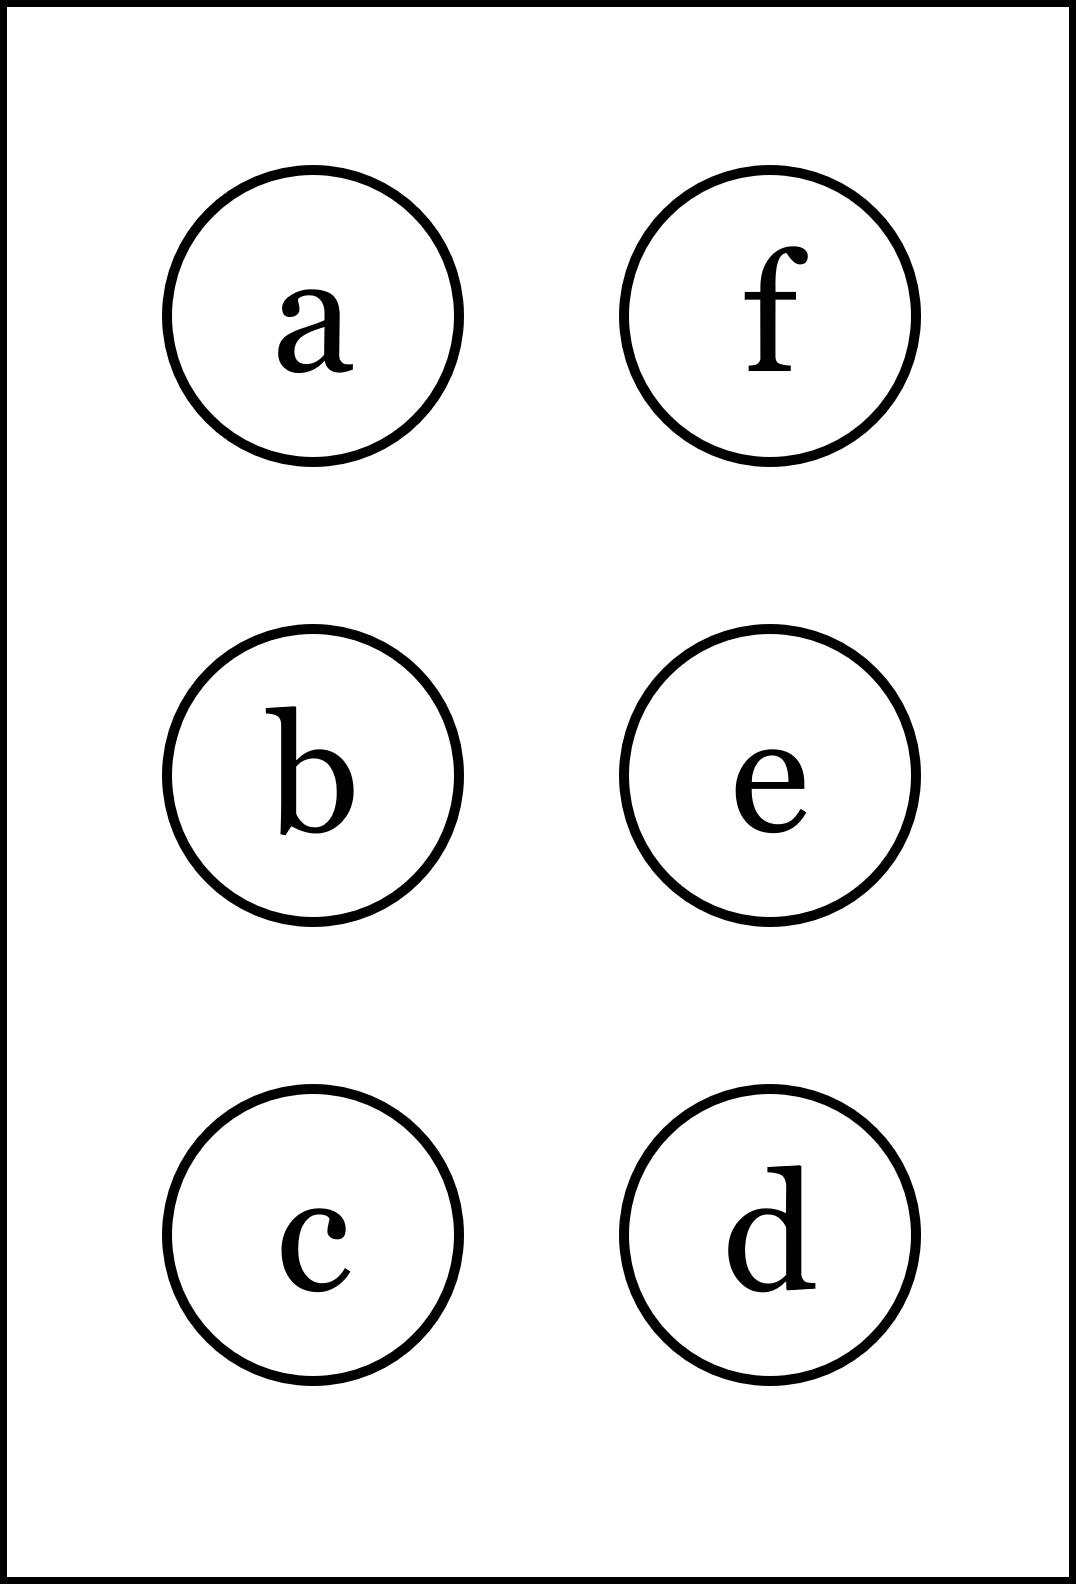
\includegraphics[height=40mm]{../images/braille.png}
{\small Písmeno Braillovej abecedy}
\end{center}
\end{minipage}
\end{center}
\end{minipage}
&
\begin{minipage}[c][104.5mm][t]{0.5\linewidth}
\begin{center}
\vspace{7mm}
{\huge Stacionární body, skupina \textit{Alpha $\alpha$} -\romannumeral2}\\[5mm]
\textit{Jméno:}\phantom{xxxxxxxxxxxxxxxxxxxxxxxxxxxxxxxxxxxxxxxxxxxxxxxxxxxxxxxxxxxxxxxxx}\\[5mm]
\begin{minipage}{0.95\linewidth}
\begin{center}
{\small V \textbf{(a)} zjisti jestli $f(x)$ \textbf{roste} v bode $x_0$. V \textbf{(b)} zjisti jestli je $f(x)$ v bode $x_0$ \textbf{ryze konvexní}.\\V \textbf{(c)} spočti \textbf{součet} x-ových souřadnic stacionárního a inflexního bodu. V \textbf{(d)} najdi x-ovou souřadnici stacionárního bodu a rozhodli jestli to je \textbf{lomax, lomin či inflex}.\\Pokud se výsledky shodujú s těmi za otazníky, tak napravo obarvi příslušející kroužek načerno.\\\textbf{Spolu odevzdejte výsledné slovo}}.
\end{center}
\end{minipage}
\\[1mm]
\begin{minipage}{0.79\linewidth}
\begin{center}
\begin{varwidth}{\linewidth}
\begin{enumerate}
\normalsize
\item $f(x)=\cfrac{4x^2-8x+1}{2x+3}\enspace , \enspace x_0=2$\quad \dotfill\; ???\;\dotfill \quad \text{ne}
\item $f(x)=2x^4-2x^3-4x^2-4x+1\enspace , \enspace x_0=3$\quad \dotfill\; ???\;\dotfill \quad \text{ano}
\item $f(x)=-xe^{x}$\quad \dotfill\; ???\;\dotfill \quad $-3$
\item $f(x)=\sqrt{4x^2-2x+1}$\quad \dotfill\; ???\;\dotfill \quad $\nicefrac{1}{4}\enspace , \enspace\mathrm{lomax}$
\item \quad \dotfill\; ???\;\dotfill \quad nebarvi
\item \quad \dotfill\; ???\;\dotfill \quad vybarvi
\end{enumerate}
\end{varwidth}
\end{center}
\end{minipage}
\begin{minipage}{0.20\linewidth}
\begin{center}
{\Huge\bfseries 2.} \\[2mm]
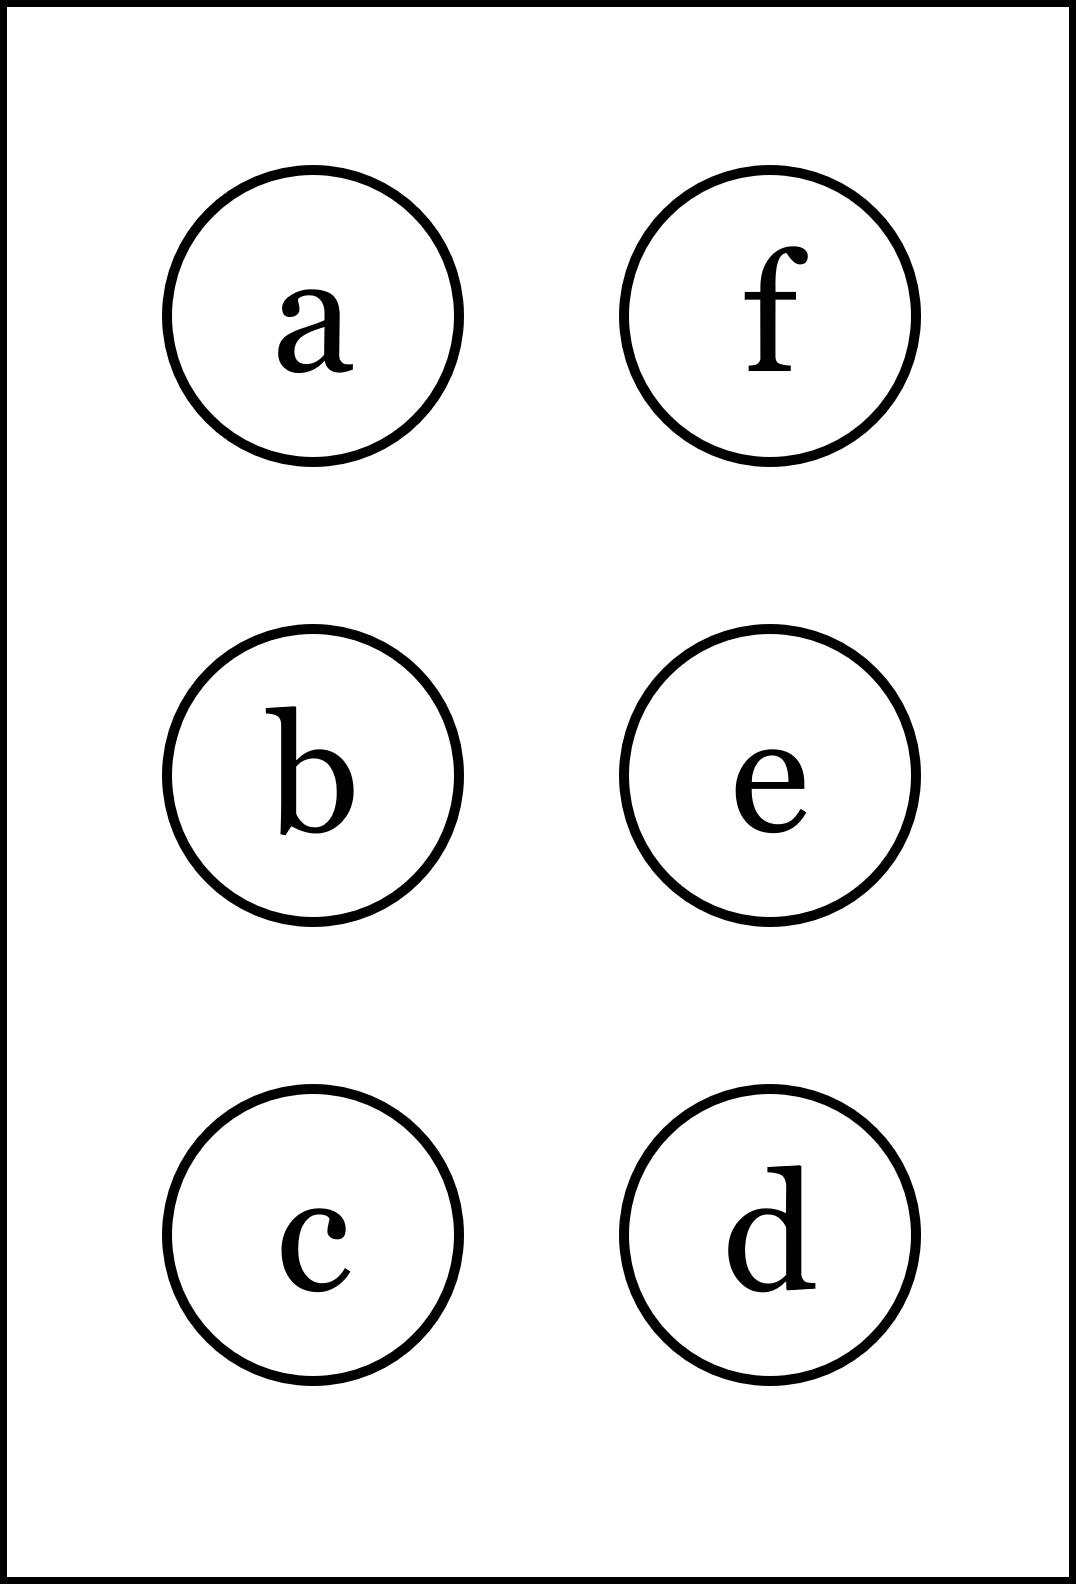
\includegraphics[height=40mm]{../images/braille.png}
{\small Písmeno Braillovej abecedy}
\end{center}
\end{minipage}
\end{center}
\end{minipage}
\\ \hdashline
\begin{minipage}[c][104.5mm][t]{0.5\linewidth}
\begin{center}
\vspace{7mm}
{\huge Stacionární body, skupina \textit{Alpha $\alpha$} -\romannumeral3}\\[5mm]
\textit{Jméno:}\phantom{xxxxxxxxxxxxxxxxxxxxxxxxxxxxxxxxxxxxxxxxxxxxxxxxxxxxxxxxxxxxxxxxx}\\[5mm]
\begin{minipage}{0.95\linewidth}
\begin{center}
{\small V \textbf{(a)} zjisti jestli $f(x)$ \textbf{roste} v bode $x_0$. V \textbf{(b)} zjisti jestli je $f(x)$ v bode $x_0$ \textbf{ryze konvexní}.\\V \textbf{(c)} spočti \textbf{součet} x-ových souřadnic stacionárního a inflexního bodu. V \textbf{(d)} najdi x-ovou souřadnici stacionárního bodu a rozhodli jestli to je \textbf{lomax, lomin či inflex}.\\Pokud se výsledky shodujú s těmi za otazníky, tak napravo obarvi příslušející kroužek načerno.\\\textbf{Spolu odevzdejte výsledné slovo}}.
\end{center}
\end{minipage}
\\[1mm]
\begin{minipage}{0.79\linewidth}
\begin{center}
\begin{varwidth}{\linewidth}
\begin{enumerate}
\normalsize
\item $f(x)=\cfrac{x^2-7x+2}{-3x-1}\enspace , \enspace x_0=2$\quad \dotfill\; ???\;\dotfill \quad \text{ano}
\item $f(x)=6x^4-7x^3+2x^2+3x-8\enspace , \enspace x_0=2$\quad \dotfill\; ???\;\dotfill \quad \text{ano}
\item $f(x)=xe^{3x}$\quad \dotfill\; ???\;\dotfill \quad $-1$
\item $f(x)=\sqrt{x^2+3x+5}$\quad \dotfill\; ???\;\dotfill \quad $\nicefrac{-3}{2}\enspace , \enspace\mathrm{lomax}$
\item \quad \dotfill\; ???\;\dotfill \quad vybarvi
\item \quad \dotfill\; ???\;\dotfill \quad vybarvi
\end{enumerate}
\end{varwidth}
\end{center}
\end{minipage}
\begin{minipage}{0.20\linewidth}
\begin{center}
{\Huge\bfseries 3.} \\[2mm]
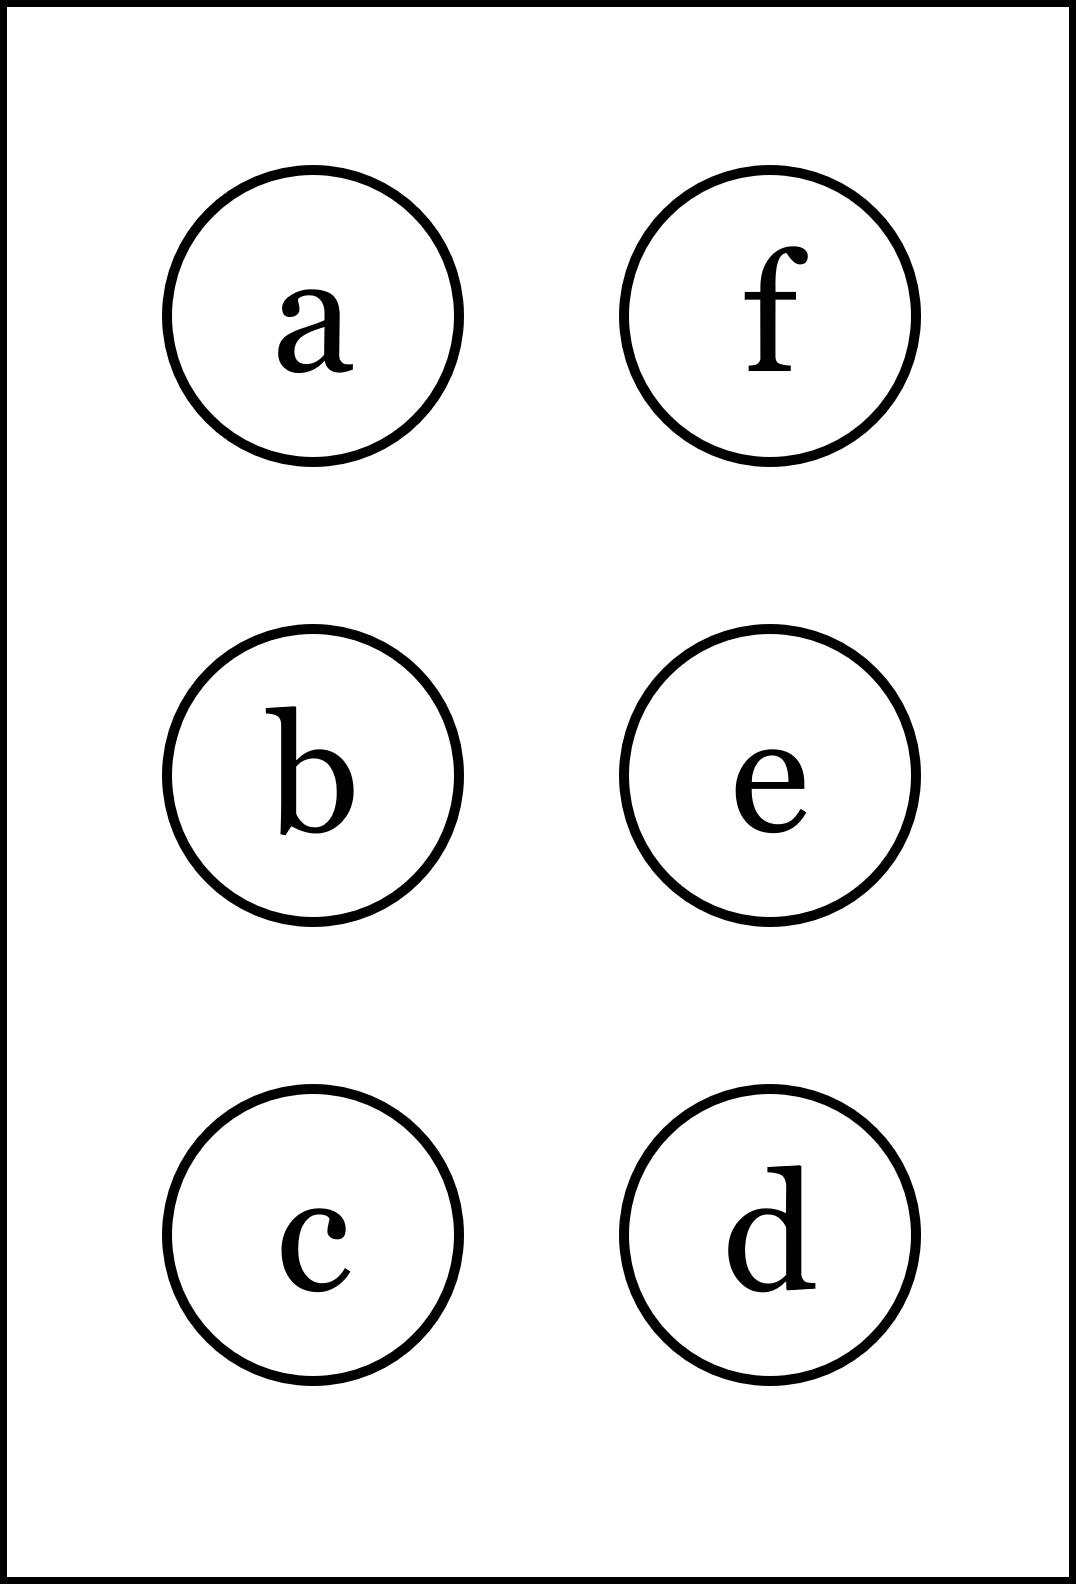
\includegraphics[height=40mm]{../images/braille.png}
{\small Písmeno Braillovej abecedy}
\end{center}
\end{minipage}
\end{center}
\end{minipage}
&
\begin{minipage}[c][104.5mm][t]{0.5\linewidth}
\begin{center}
\vspace{7mm}
{\huge Stacionární body, skupina \textit{Alpha $\alpha$} -\romannumeral4}\\[5mm]
\textit{Jméno:}\phantom{xxxxxxxxxxxxxxxxxxxxxxxxxxxxxxxxxxxxxxxxxxxxxxxxxxxxxxxxxxxxxxxxx}\\[5mm]
\begin{minipage}{0.95\linewidth}
\begin{center}
{\small V \textbf{(a)} zjisti jestli $f(x)$ \textbf{roste} v bode $x_0$. V \textbf{(b)} zjisti jestli je $f(x)$ v bode $x_0$ \textbf{ryze konvexní}.\\V \textbf{(c)} spočti \textbf{součet} x-ových souřadnic stacionárního a inflexního bodu. V \textbf{(d)} najdi x-ovou souřadnici stacionárního bodu a rozhodli jestli to je \textbf{lomax, lomin či inflex}.\\Pokud se výsledky shodujú s těmi za otazníky, tak napravo obarvi příslušející kroužek načerno.\\\textbf{Spolu odevzdejte výsledné slovo}}.
\end{center}
\end{minipage}
\\[1mm]
\begin{minipage}{0.79\linewidth}
\begin{center}
\begin{varwidth}{\linewidth}
\begin{enumerate}
\normalsize
\item $f(x)=\cfrac{x^2+5x-2}{x+3}\enspace , \enspace x_0=-8$\quad \dotfill\; ???\;\dotfill \quad \text{ano}
\item $f(x)=x^4+6x^3+2x^2-x-4\enspace , \enspace x_0=1$\quad \dotfill\; ???\;\dotfill \quad \text{ne}
\item $f(x)=-4xe^{-5x}$\quad \dotfill\; ???\;\dotfill \quad $\nicefrac{-1}{5}$
\item $f(x)=\sqrt{4x^2-2x+3}$\quad \dotfill\; ???\;\dotfill \quad $\nicefrac{1}{4}\enspace , \enspace\mathrm{inflex}$
\item \quad \dotfill\; ???\;\dotfill \quad nebarvi
\item \quad \dotfill\; ???\;\dotfill \quad nebarvi
\end{enumerate}
\end{varwidth}
\end{center}
\end{minipage}
\begin{minipage}{0.20\linewidth}
\begin{center}
{\Huge\bfseries 4.} \\[2mm]
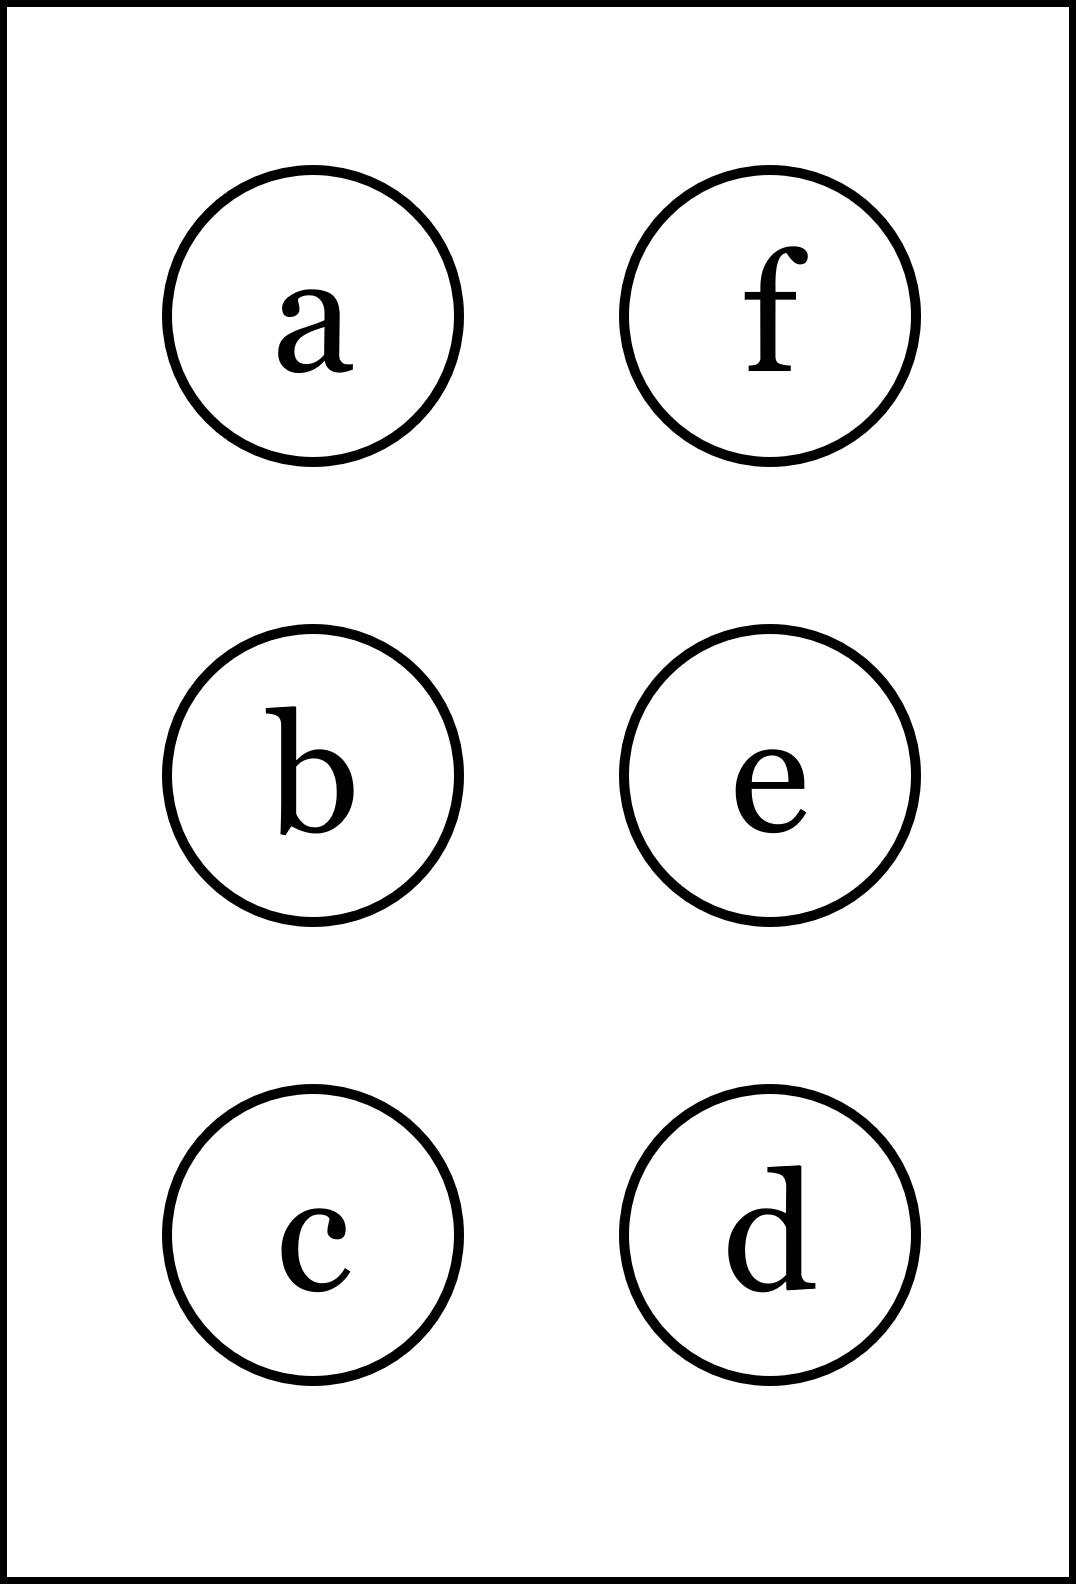
\includegraphics[height=40mm]{../images/braille.png}
{\small Písmeno Braillovej abecedy}
\end{center}
\end{minipage}
\end{center}
\end{minipage}
%
\end{tabular}
\newpage
\thispagestyle{empty}
\begin{tabular}{c:c}
\begin{minipage}[c][104.5mm][t]{0.5\linewidth}
\begin{center}
\vspace{7mm}
{\huge Stacionární body, skupina \textit{Beta $\beta$} -\romannumeral1}\\[5mm]
\textit{Jméno:}\phantom{xxxxxxxxxxxxxxxxxxxxxxxxxxxxxxxxxxxxxxxxxxxxxxxxxxxxxxxxxxxxxxxxx}\\[5mm]
\begin{minipage}{0.95\linewidth}
\begin{center}
{\small V \textbf{(a)} zjisti jestli $f(x)$ \textbf{roste} v bode $x_0$. V \textbf{(b)} zjisti jestli je $f(x)$ v bode $x_0$ \textbf{ryze konvexní}.\\V \textbf{(c)} spočti \textbf{součet} x-ových souřadnic stacionárního a inflexního bodu. V \textbf{(d)} najdi x-ovou souřadnici stacionárního bodu a rozhodli jestli to je \textbf{lomax, lomin či inflex}.\\Pokud se výsledky shodujú s těmi za otazníky, tak napravo obarvi příslušející kroužek načerno.\\\textbf{Spolu odevzdejte výsledné slovo}}.
\end{center}
\end{minipage}
\\[1mm]
\begin{minipage}{0.79\linewidth}
\begin{center}
\begin{varwidth}{\linewidth}
\begin{enumerate}
\normalsize
\item $f(x)=\cfrac{-x^2-x+2}{9x-1}\enspace , \enspace x_0=-3$\quad \dotfill\; ???\;\dotfill \quad \text{ano}
\item $f(x)=-3x^4+3x^3-x^2-6x+4\enspace , \enspace x_0=-3$\quad \dotfill\; ???\;\dotfill \quad \text{ne}
\item $f(x)=-2xe^{-5x}$\quad \dotfill\; ???\;\dotfill \quad $\nicefrac{-1}{5}$
\item $f(x)=\sqrt{5x^2+x+2}$\quad \dotfill\; ???\;\dotfill \quad $\nicefrac{-1}{10}\enspace , \enspace\mathrm{lomax}$
\item \quad \dotfill\; ???\;\dotfill \quad nebarvi
\item \quad \dotfill\; ???\;\dotfill \quad vybarvi
\end{enumerate}
\end{varwidth}
\end{center}
\end{minipage}
\begin{minipage}{0.20\linewidth}
\begin{center}
{\Huge\bfseries 1.} \\[2mm]
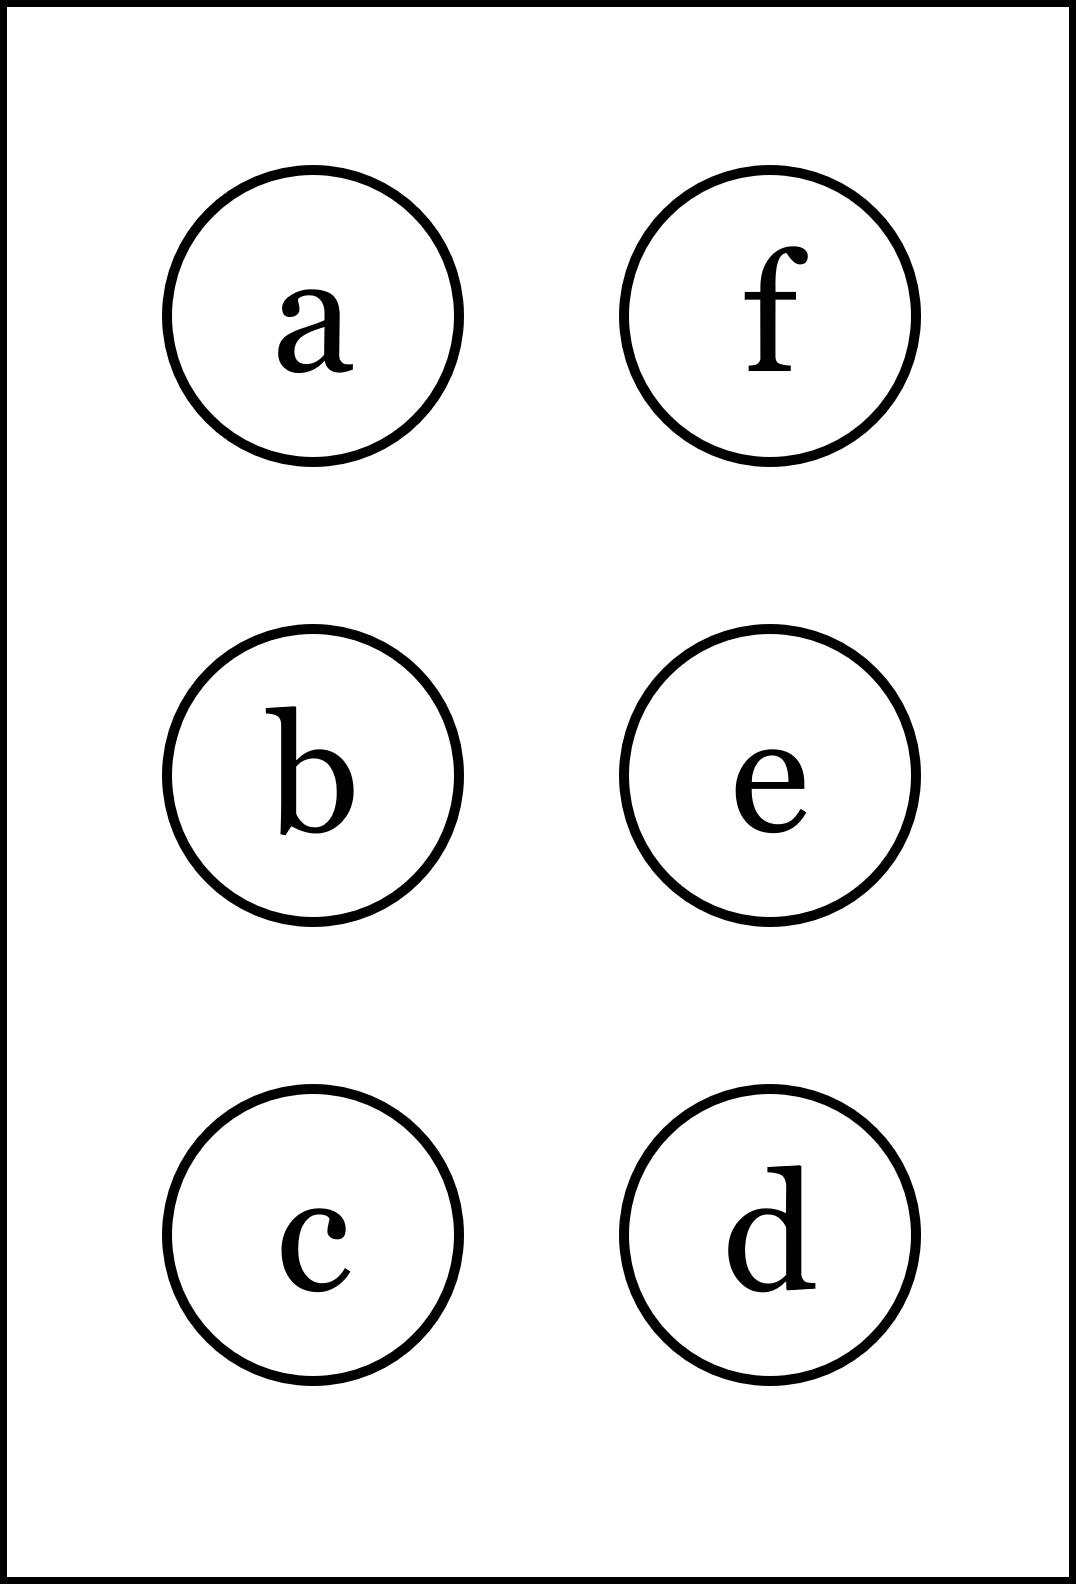
\includegraphics[height=40mm]{../images/braille.png}
{\small Písmeno Braillovej abecedy}
\end{center}
\end{minipage}
\end{center}
\end{minipage}
&
\begin{minipage}[c][104.5mm][t]{0.5\linewidth}
\begin{center}
\vspace{7mm}
{\huge Stacionární body, skupina \textit{Beta $\beta$} -\romannumeral2}\\[5mm]
\textit{Jméno:}\phantom{xxxxxxxxxxxxxxxxxxxxxxxxxxxxxxxxxxxxxxxxxxxxxxxxxxxxxxxxxxxxxxxxx}\\[5mm]
\begin{minipage}{0.95\linewidth}
\begin{center}
{\small V \textbf{(a)} zjisti jestli $f(x)$ \textbf{roste} v bode $x_0$. V \textbf{(b)} zjisti jestli je $f(x)$ v bode $x_0$ \textbf{ryze konvexní}.\\V \textbf{(c)} spočti \textbf{součet} x-ových souřadnic stacionárního a inflexního bodu. V \textbf{(d)} najdi x-ovou souřadnici stacionárního bodu a rozhodli jestli to je \textbf{lomax, lomin či inflex}.\\Pokud se výsledky shodujú s těmi za otazníky, tak napravo obarvi příslušející kroužek načerno.\\\textbf{Spolu odevzdejte výsledné slovo}}.
\end{center}
\end{minipage}
\\[1mm]
\begin{minipage}{0.79\linewidth}
\begin{center}
\begin{varwidth}{\linewidth}
\begin{enumerate}
\normalsize
\item $f(x)=\cfrac{-x^2-3x-5}{2x-3}\enspace , \enspace x_0=5$\quad \dotfill\; ???\;\dotfill \quad \text{ne}
\item $f(x)=-2x^4-8x^3+x^2-3x-6\enspace , \enspace x_0=2$\quad \dotfill\; ???\;\dotfill \quad \text{ne}
\item $f(x)=4xe^{x}$\quad \dotfill\; ???\;\dotfill \quad $1$
\item $f(x)=\sqrt{3x^2+3x+2}$\quad \dotfill\; ???\;\dotfill \quad $\nicefrac{-1}{2}\enspace , \enspace\mathrm{lomax}$
\item \quad \dotfill\; ???\;\dotfill \quad vybarvi
\item \quad \dotfill\; ???\;\dotfill \quad vybarvi
\end{enumerate}
\end{varwidth}
\end{center}
\end{minipage}
\begin{minipage}{0.20\linewidth}
\begin{center}
{\Huge\bfseries 2.} \\[2mm]
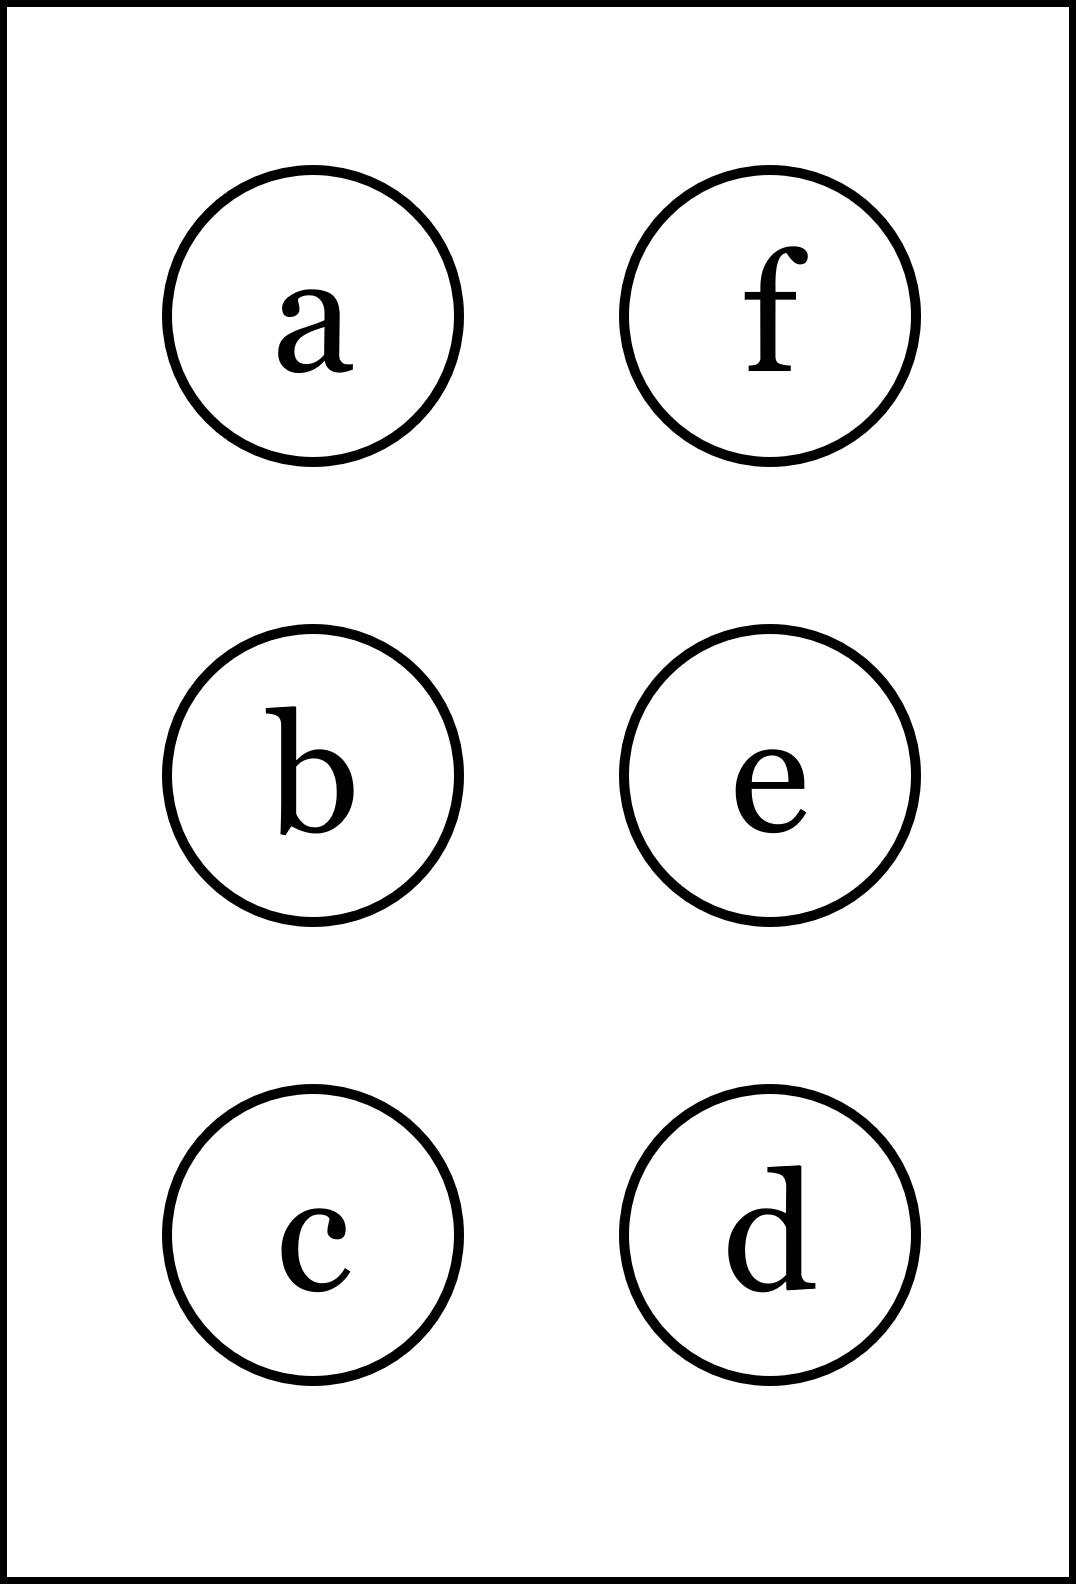
\includegraphics[height=40mm]{../images/braille.png}
{\small Písmeno Braillovej abecedy}
\end{center}
\end{minipage}
\end{center}
\end{minipage}
\\ \hdashline
\begin{minipage}[c][104.5mm][t]{0.5\linewidth}
\begin{center}
\vspace{7mm}
{\huge Stacionární body, skupina \textit{Beta $\beta$} -\romannumeral3}\\[5mm]
\textit{Jméno:}\phantom{xxxxxxxxxxxxxxxxxxxxxxxxxxxxxxxxxxxxxxxxxxxxxxxxxxxxxxxxxxxxxxxxx}\\[5mm]
\begin{minipage}{0.95\linewidth}
\begin{center}
{\small V \textbf{(a)} zjisti jestli $f(x)$ \textbf{roste} v bode $x_0$. V \textbf{(b)} zjisti jestli je $f(x)$ v bode $x_0$ \textbf{ryze konvexní}.\\V \textbf{(c)} spočti \textbf{součet} x-ových souřadnic stacionárního a inflexního bodu. V \textbf{(d)} najdi x-ovou souřadnici stacionárního bodu a rozhodli jestli to je \textbf{lomax, lomin či inflex}.\\Pokud se výsledky shodujú s těmi za otazníky, tak napravo obarvi příslušející kroužek načerno.\\\textbf{Spolu odevzdejte výsledné slovo}}.
\end{center}
\end{minipage}
\\[1mm]
\begin{minipage}{0.79\linewidth}
\begin{center}
\begin{varwidth}{\linewidth}
\begin{enumerate}
\normalsize
\item $f(x)=\cfrac{3x^2+3x-3}{x-1}\enspace , \enspace x_0=5$\quad \dotfill\; ???\;\dotfill \quad \text{ano}
\item $f(x)=3x^4+2x^3+x^2+3x-6\enspace , \enspace x_0=1$\quad \dotfill\; ???\;\dotfill \quad \text{ano}
\item $f(x)=6xe^{-2x}$\quad \dotfill\; ???\;\dotfill \quad $\nicefrac{3}{2}$
\item $f(x)=\sqrt{2x^2+2x+3}$\quad \dotfill\; ???\;\dotfill \quad $\nicefrac{-1}{2}\enspace , \enspace\mathrm{lomax}$
\item \quad \dotfill\; ???\;\dotfill \quad nebarvi
\item \quad \dotfill\; ???\;\dotfill \quad nebarvi
\end{enumerate}
\end{varwidth}
\end{center}
\end{minipage}
\begin{minipage}{0.20\linewidth}
\begin{center}
{\Huge\bfseries 3.} \\[2mm]
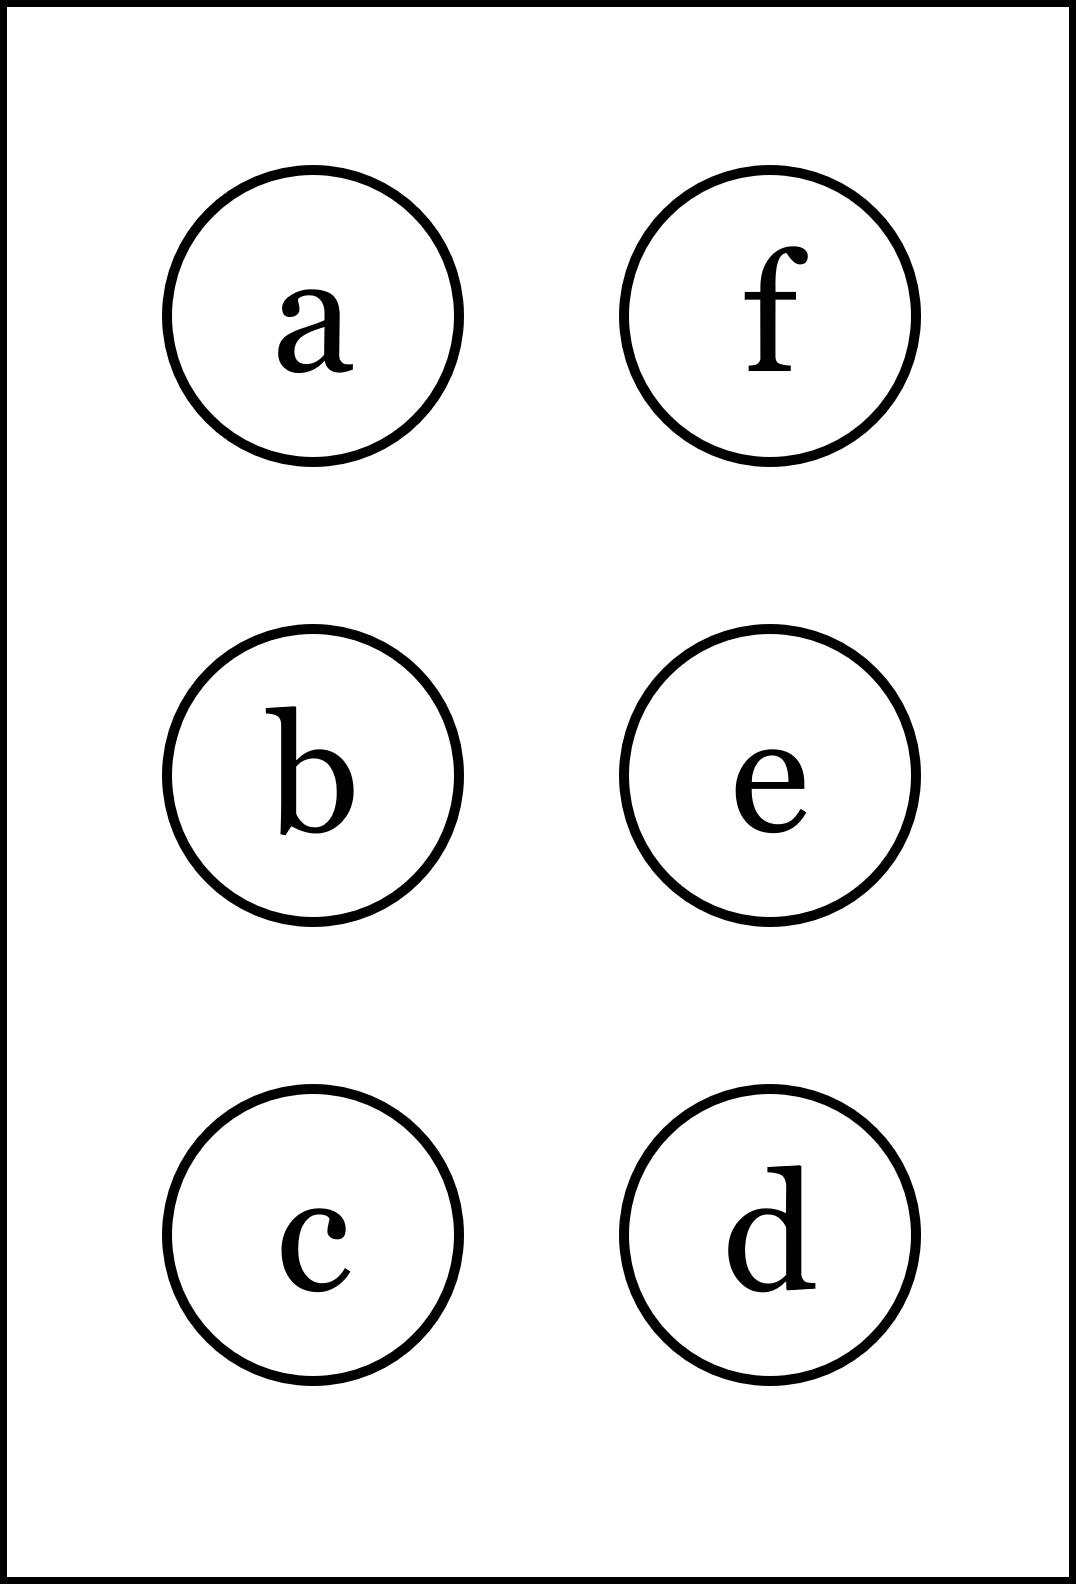
\includegraphics[height=40mm]{../images/braille.png}
{\small Písmeno Braillovej abecedy}
\end{center}
\end{minipage}
\end{center}
\end{minipage}
&
\begin{minipage}[c][104.5mm][t]{0.5\linewidth}
\begin{center}
\vspace{7mm}
{\huge Stacionární body, skupina \textit{Beta $\beta$} -\romannumeral4}\\[5mm]
\textit{Jméno:}\phantom{xxxxxxxxxxxxxxxxxxxxxxxxxxxxxxxxxxxxxxxxxxxxxxxxxxxxxxxxxxxxxxxxx}\\[5mm]
\begin{minipage}{0.95\linewidth}
\begin{center}
{\small V \textbf{(a)} zjisti jestli $f(x)$ \textbf{roste} v bode $x_0$. V \textbf{(b)} zjisti jestli je $f(x)$ v bode $x_0$ \textbf{ryze konvexní}.\\V \textbf{(c)} spočti \textbf{součet} x-ových souřadnic stacionárního a inflexního bodu. V \textbf{(d)} najdi x-ovou souřadnici stacionárního bodu a rozhodli jestli to je \textbf{lomax, lomin či inflex}.\\Pokud se výsledky shodujú s těmi za otazníky, tak napravo obarvi příslušející kroužek načerno.\\\textbf{Spolu odevzdejte výsledné slovo}}.
\end{center}
\end{minipage}
\\[1mm]
\begin{minipage}{0.79\linewidth}
\begin{center}
\begin{varwidth}{\linewidth}
\begin{enumerate}
\normalsize
\item $f(x)=\cfrac{-6x^2-5x-3}{x-3}\enspace , \enspace x_0=2$\quad \dotfill\; ???\;\dotfill \quad \text{ano}
\item $f(x)=-2x^4-5x^3+3x^2-x+2\enspace , \enspace x_0=-2$\quad \dotfill\; ???\;\dotfill \quad \text{ano}
\item $f(x)=9xe^{-2x}$\quad \dotfill\; ???\;\dotfill \quad $\nicefrac{3}{2}$
\item $f(x)=\sqrt{x^2+x+3}$\quad \dotfill\; ???\;\dotfill \quad $\nicefrac{-1}{2}\enspace , \enspace \mathrm{lomin}$
\item \quad \dotfill\; ???\;\dotfill \quad nebarvi
\item \quad \dotfill\; ???\;\dotfill \quad nebarvi
\end{enumerate}
\end{varwidth}
\end{center}
\end{minipage}
\begin{minipage}{0.20\linewidth}
\begin{center}
{\Huge\bfseries 4.} \\[2mm]
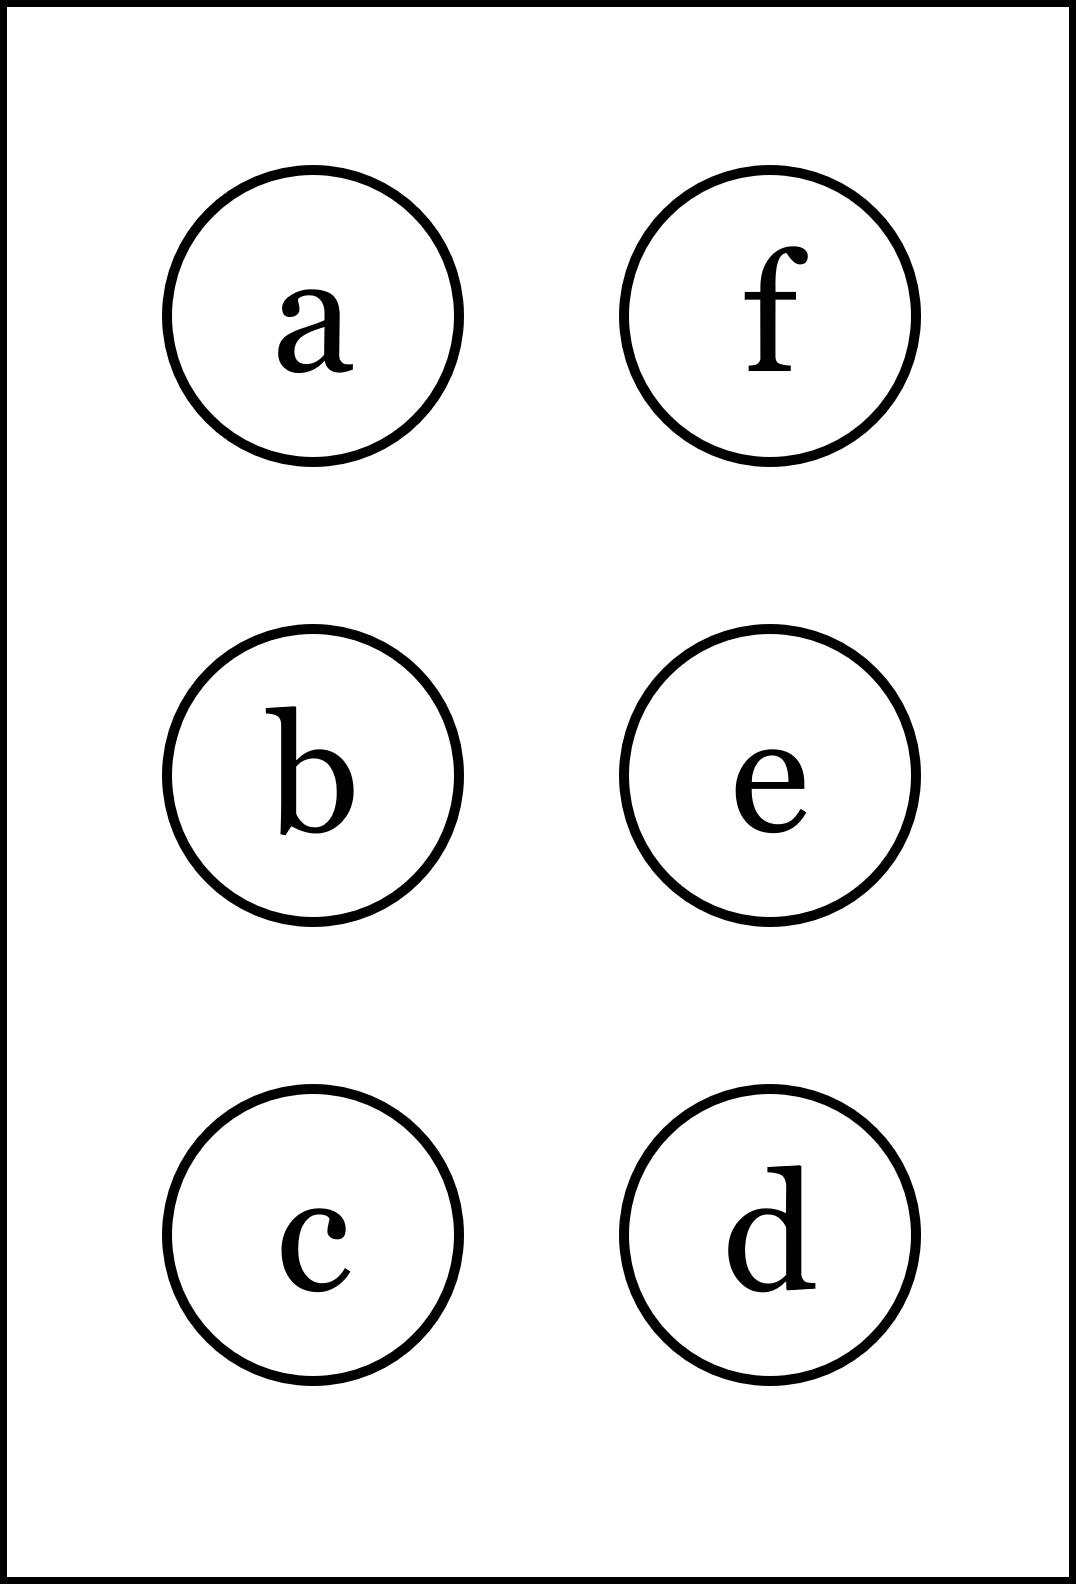
\includegraphics[height=40mm]{../images/braille.png}
{\small Písmeno Braillovej abecedy}
\end{center}
\end{minipage}
\end{center}
\end{minipage}
%
\end{tabular}
\newpage
\thispagestyle{empty}
\begin{tabular}{c:c}
\begin{minipage}[c][104.5mm][t]{0.5\linewidth}
\begin{center}
\vspace{7mm}
{\huge Stacionární body, skupina \textit{Gamma $\gamma$} -\romannumeral1}\\[5mm]
\textit{Jméno:}\phantom{xxxxxxxxxxxxxxxxxxxxxxxxxxxxxxxxxxxxxxxxxxxxxxxxxxxxxxxxxxxxxxxxx}\\[5mm]
\begin{minipage}{0.95\linewidth}
\begin{center}
{\small V \textbf{(a)} zjisti jestli $f(x)$ \textbf{roste} v bode $x_0$. V \textbf{(b)} zjisti jestli je $f(x)$ v bode $x_0$ \textbf{ryze konvexní}.\\V \textbf{(c)} spočti \textbf{součet} x-ových souřadnic stacionárního a inflexního bodu. V \textbf{(d)} najdi x-ovou souřadnici stacionárního bodu a rozhodli jestli to je \textbf{lomax, lomin či inflex}.\\Pokud se výsledky shodujú s těmi za otazníky, tak napravo obarvi příslušející kroužek načerno.\\\textbf{Spolu odevzdejte výsledné slovo}}.
\end{center}
\end{minipage}
\\[1mm]
\begin{minipage}{0.79\linewidth}
\begin{center}
\begin{varwidth}{\linewidth}
\begin{enumerate}
\normalsize
\item $f(x)=\cfrac{4x^2+x-1}{4x-4}\enspace , \enspace x_0=-1$\quad \dotfill\; ???\;\dotfill \quad \text{ano}
\item $f(x)=-2x^4-6x^3-x^2+2x-1\enspace , \enspace x_0=-1$\quad \dotfill\; ???\;\dotfill \quad \text{ano}
\item $f(x)=-4xe^{-2x}$\quad \dotfill\; ???\;\dotfill \quad $\nicefrac{3}{2}$
\item $f(x)=\sqrt{x^2-x+3}$\quad \dotfill\; ???\;\dotfill \quad $\nicefrac{1}{2}\enspace , \enspace\mathrm{lomax}$
\item \quad \dotfill\; ???\;\dotfill \quad vybarvi
\item \quad \dotfill\; ???\;\dotfill \quad nebarvi
\end{enumerate}
\end{varwidth}
\end{center}
\end{minipage}
\begin{minipage}{0.20\linewidth}
\begin{center}
{\Huge\bfseries 1.} \\[2mm]
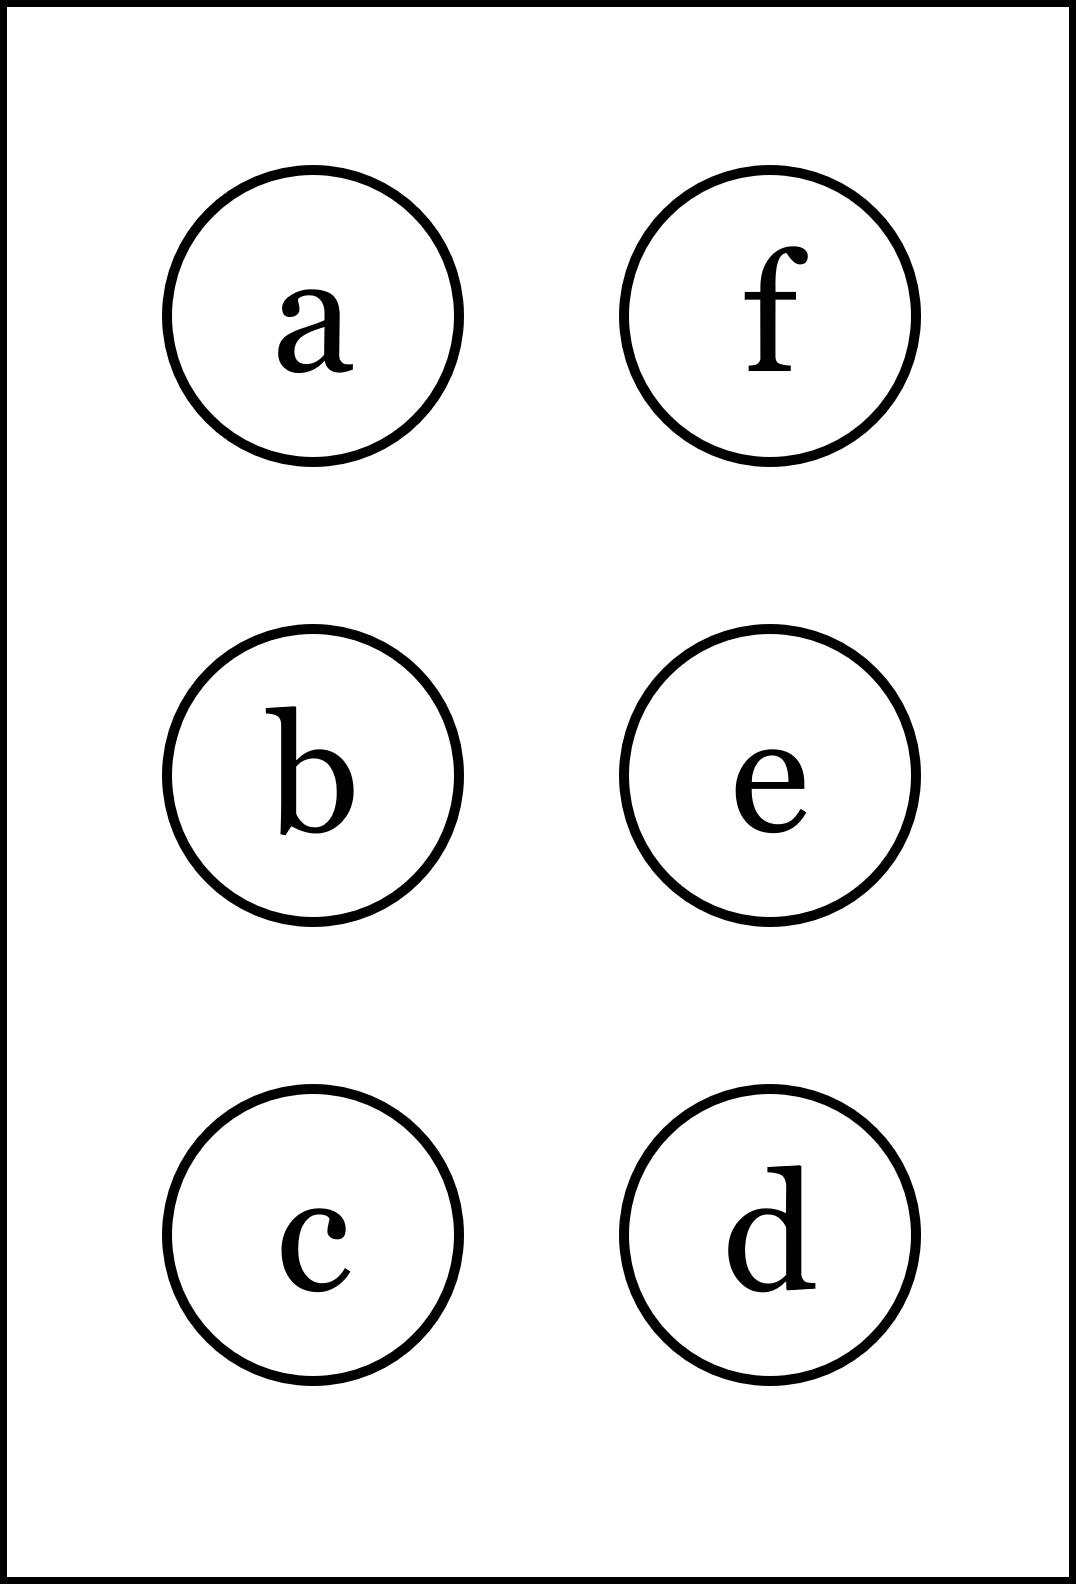
\includegraphics[height=40mm]{../images/braille.png}
{\small Písmeno Braillovej abecedy}
\end{center}
\end{minipage}
\end{center}
\end{minipage}
&
\begin{minipage}[c][104.5mm][t]{0.5\linewidth}
\begin{center}
\vspace{7mm}
{\huge Stacionární body, skupina \textit{Gamma $\gamma$} -\romannumeral2}\\[5mm]
\textit{Jméno:}\phantom{xxxxxxxxxxxxxxxxxxxxxxxxxxxxxxxxxxxxxxxxxxxxxxxxxxxxxxxxxxxxxxxxx}\\[5mm]
\begin{minipage}{0.95\linewidth}
\begin{center}
{\small V \textbf{(a)} zjisti jestli $f(x)$ \textbf{roste} v bode $x_0$. V \textbf{(b)} zjisti jestli je $f(x)$ v bode $x_0$ \textbf{ryze konvexní}.\\V \textbf{(c)} spočti \textbf{součet} x-ových souřadnic stacionárního a inflexního bodu. V \textbf{(d)} najdi x-ovou souřadnici stacionárního bodu a rozhodli jestli to je \textbf{lomax, lomin či inflex}.\\Pokud se výsledky shodujú s těmi za otazníky, tak napravo obarvi příslušející kroužek načerno.\\\textbf{Spolu odevzdejte výsledné slovo}}.
\end{center}
\end{minipage}
\\[1mm]
\begin{minipage}{0.79\linewidth}
\begin{center}
\begin{varwidth}{\linewidth}
\begin{enumerate}
\normalsize
\item $f(x)=\cfrac{-3x^2+2x-8}{2x+5}\enspace , \enspace x_0=-1$\quad \dotfill\; ???\;\dotfill \quad \text{ano}
\item $f(x)=-8x^4-8x^3-2x^2+4x+6\enspace , \enspace x_0=-2$\quad \dotfill\; ???\;\dotfill \quad \text{ano}
\item $f(x)=-6xe^{-5x}$\quad \dotfill\; ???\;\dotfill \quad $\nicefrac{-1}{5}$
\item $f(x)=\sqrt{x^2+2x+2}$\quad \dotfill\; ???\;\dotfill \quad $-1\enspace , \enspace\mathrm{lomax}$
\item \quad \dotfill\; ???\;\dotfill \quad vybarvi
\item \quad \dotfill\; ???\;\dotfill \quad nebarvi
\end{enumerate}
\end{varwidth}
\end{center}
\end{minipage}
\begin{minipage}{0.20\linewidth}
\begin{center}
{\Huge\bfseries 2.} \\[2mm]
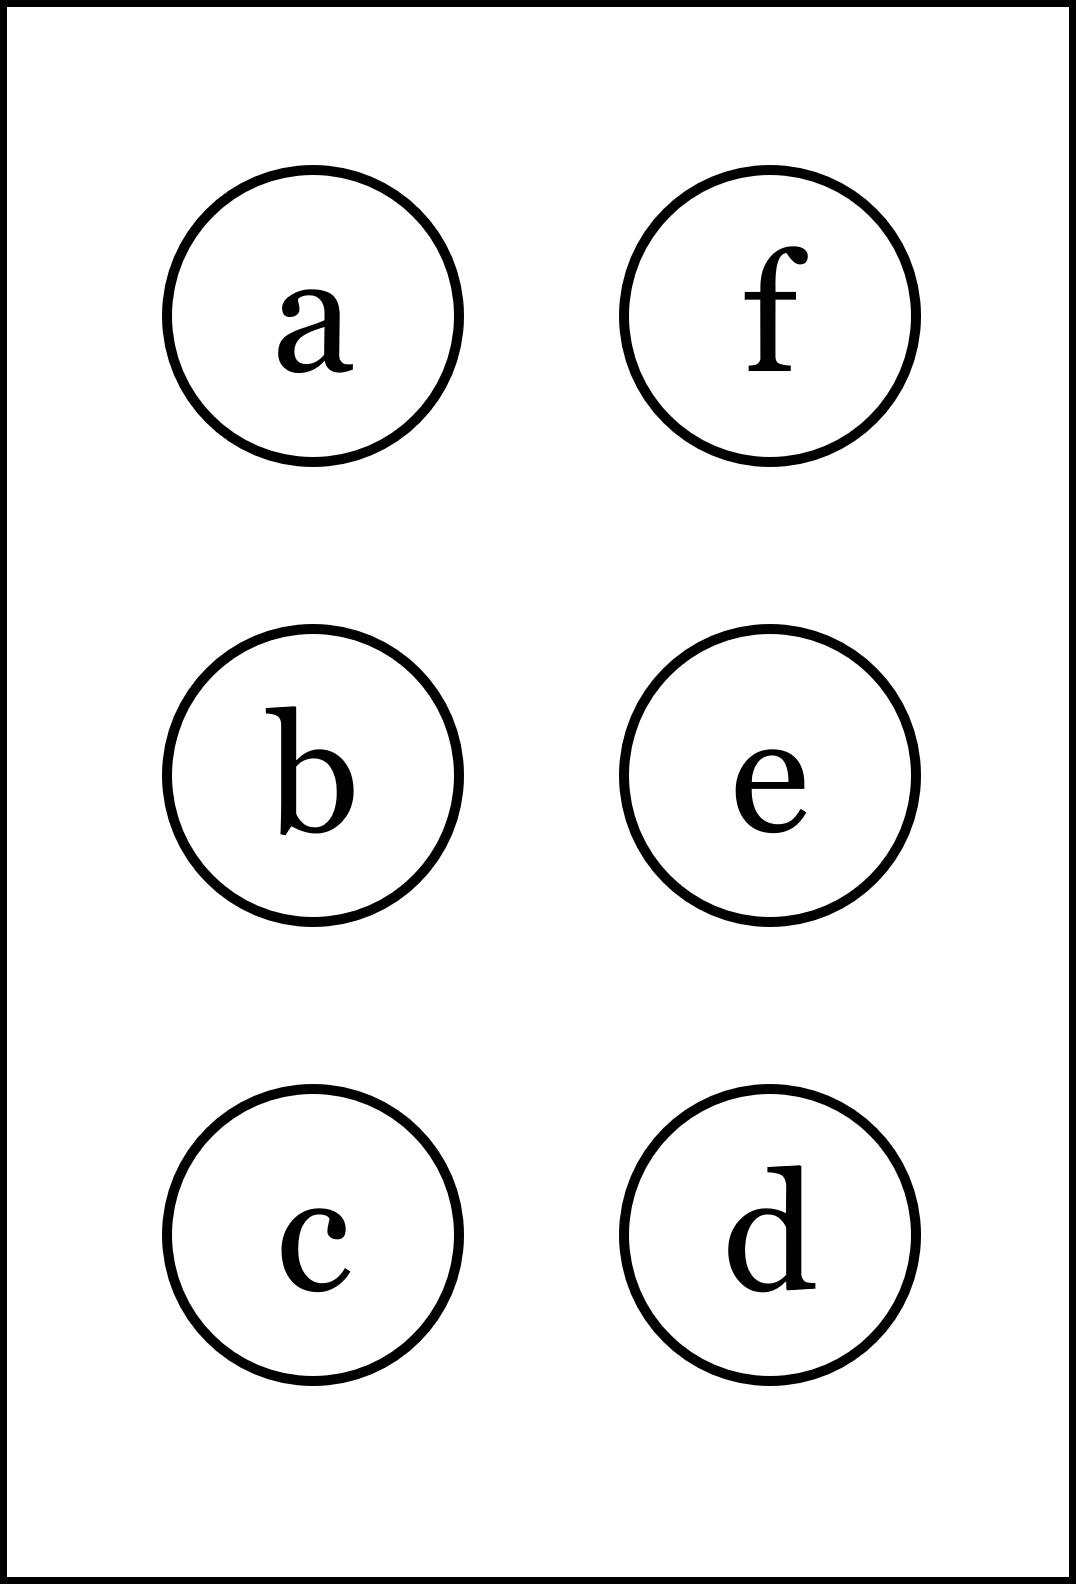
\includegraphics[height=40mm]{../images/braille.png}
{\small Písmeno Braillovej abecedy}
\end{center}
\end{minipage}
\end{center}
\end{minipage}
\\ \hdashline
\begin{minipage}[c][104.5mm][t]{0.5\linewidth}
\begin{center}
\vspace{7mm}
{\huge Stacionární body, skupina \textit{Gamma $\gamma$} -\romannumeral3}\\[5mm]
\textit{Jméno:}\phantom{xxxxxxxxxxxxxxxxxxxxxxxxxxxxxxxxxxxxxxxxxxxxxxxxxxxxxxxxxxxxxxxxx}\\[5mm]
\begin{minipage}{0.95\linewidth}
\begin{center}
{\small V \textbf{(a)} zjisti jestli $f(x)$ \textbf{roste} v bode $x_0$. V \textbf{(b)} zjisti jestli je $f(x)$ v bode $x_0$ \textbf{ryze konvexní}.\\V \textbf{(c)} spočti \textbf{součet} x-ových souřadnic stacionárního a inflexního bodu. V \textbf{(d)} najdi x-ovou souřadnici stacionárního bodu a rozhodli jestli to je \textbf{lomax, lomin či inflex}.\\Pokud se výsledky shodujú s těmi za otazníky, tak napravo obarvi příslušející kroužek načerno.\\\textbf{Spolu odevzdejte výsledné slovo}}.
\end{center}
\end{minipage}
\\[1mm]
\begin{minipage}{0.79\linewidth}
\begin{center}
\begin{varwidth}{\linewidth}
\begin{enumerate}
\normalsize
\item $f(x)=\cfrac{x^2+4x-9}{-3x-4}\enspace , \enspace x_0=1$\quad \dotfill\; ???\;\dotfill \quad \text{ne}
\item $f(x)=-9x^4+5x^3+4x^2-6x+2\enspace , \enspace x_0=1$\quad \dotfill\; ???\;\dotfill \quad \text{ne}
\item $f(x)=-3xe^{-6x}$\quad \dotfill\; ???\;\dotfill \quad $\nicefrac{1}{2}$
\item $f(x)=\sqrt{4x^2-x+2}$\quad \dotfill\; ???\;\dotfill \quad $\nicefrac{1}{8}\enspace , \enspace\mathrm{lomax}$
\item \quad \dotfill\; ???\;\dotfill \quad nebarvi
\item \quad \dotfill\; ???\;\dotfill \quad vybarvi
\end{enumerate}
\end{varwidth}
\end{center}
\end{minipage}
\begin{minipage}{0.20\linewidth}
\begin{center}
{\Huge\bfseries 3.} \\[2mm]
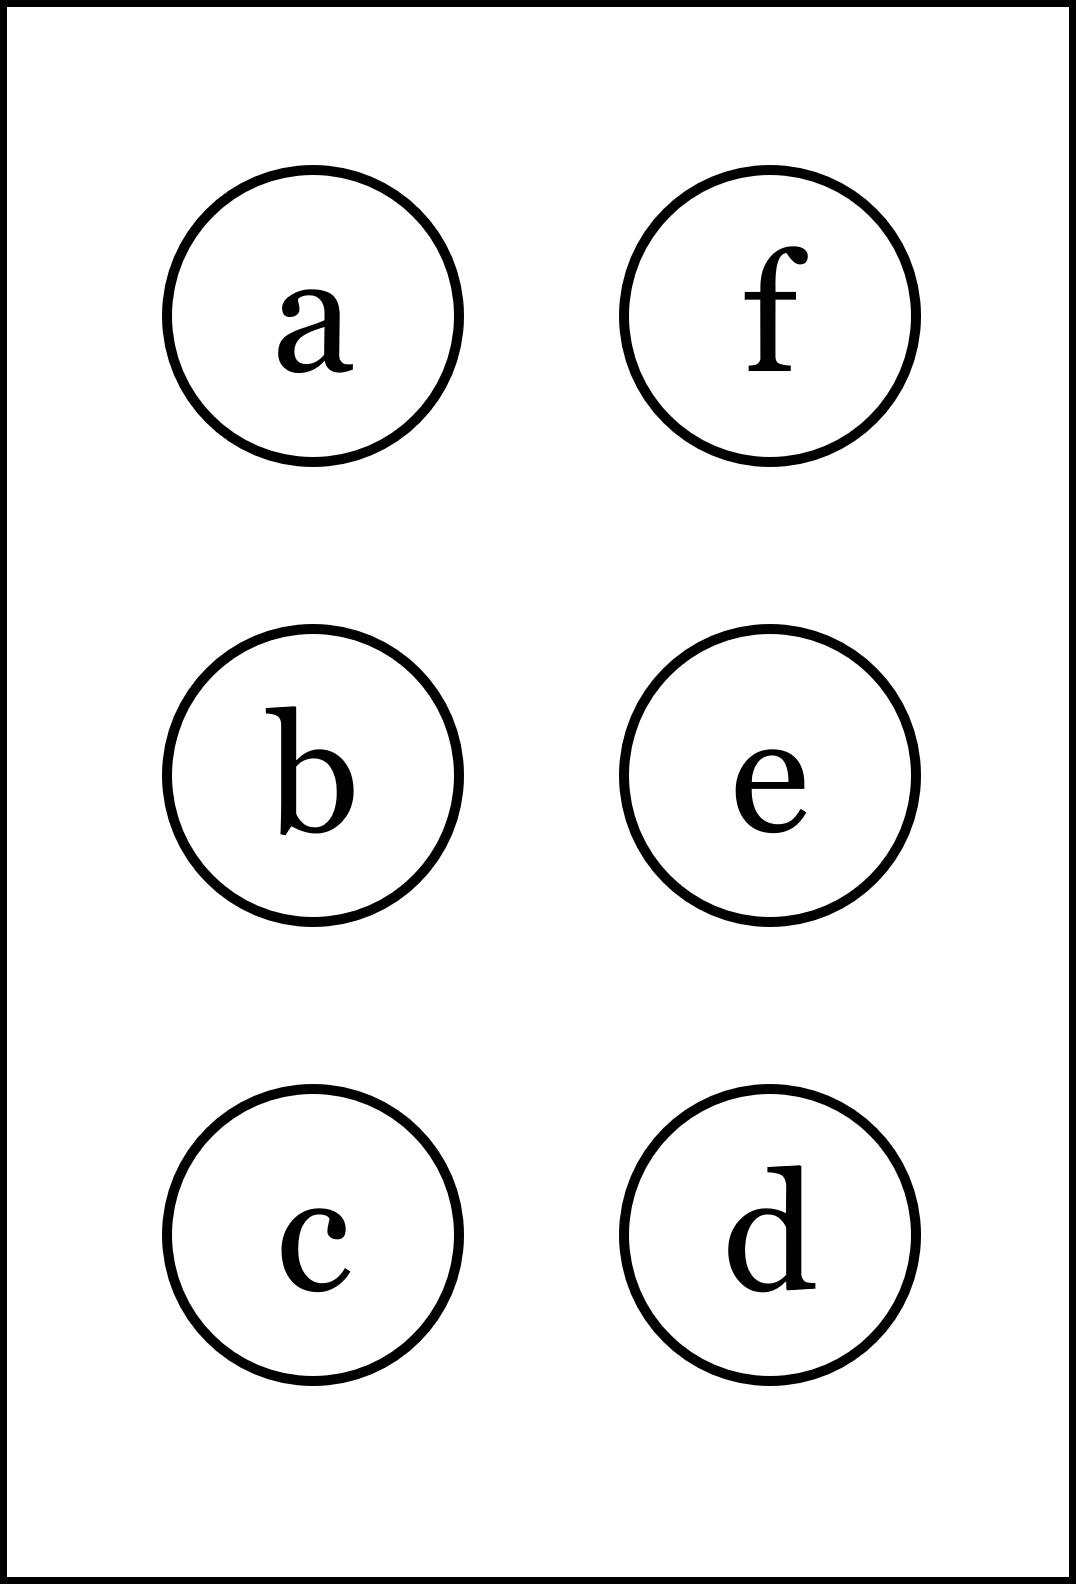
\includegraphics[height=40mm]{../images/braille.png}
{\small Písmeno Braillovej abecedy}
\end{center}
\end{minipage}
\end{center}
\end{minipage}
&
\begin{minipage}[c][104.5mm][t]{0.5\linewidth}
\begin{center}
\vspace{7mm}
{\huge Stacionární body, skupina \textit{Gamma $\gamma$} -\romannumeral4}\\[5mm]
\textit{Jméno:}\phantom{xxxxxxxxxxxxxxxxxxxxxxxxxxxxxxxxxxxxxxxxxxxxxxxxxxxxxxxxxxxxxxxxx}\\[5mm]
\begin{minipage}{0.95\linewidth}
\begin{center}
{\small V \textbf{(a)} zjisti jestli $f(x)$ \textbf{roste} v bode $x_0$. V \textbf{(b)} zjisti jestli je $f(x)$ v bode $x_0$ \textbf{ryze konvexní}.\\V \textbf{(c)} spočti \textbf{součet} x-ových souřadnic stacionárního a inflexního bodu. V \textbf{(d)} najdi x-ovou souřadnici stacionárního bodu a rozhodli jestli to je \textbf{lomax, lomin či inflex}.\\Pokud se výsledky shodujú s těmi za otazníky, tak napravo obarvi příslušející kroužek načerno.\\\textbf{Spolu odevzdejte výsledné slovo}}.
\end{center}
\end{minipage}
\\[1mm]
\begin{minipage}{0.79\linewidth}
\begin{center}
\begin{varwidth}{\linewidth}
\begin{enumerate}
\normalsize
\item $f(x)=\cfrac{-3x^2-3x+6}{-x+1}\enspace , \enspace x_0=2$\quad \dotfill\; ???\;\dotfill \quad \text{ano}
\item $f(x)=-5x^4-6x^3-3x^2-6x-1\enspace , \enspace x_0=-1$\quad \dotfill\; ???\;\dotfill \quad \text{ano}
\item $f(x)=-8xe^{-2x}$\quad \dotfill\; ???\;\dotfill \quad $\nicefrac{-1}{2}$
\item $f(x)=\sqrt{3x^2+2x+1}$\quad \dotfill\; ???\;\dotfill \quad $\nicefrac{-1}{3}\enspace , \enspace\mathrm{lomax}$
\item \quad \dotfill\; ???\;\dotfill \quad nebarvi
\item \quad \dotfill\; ???\;\dotfill \quad nebarvi
\end{enumerate}
\end{varwidth}
\end{center}
\end{minipage}
\begin{minipage}{0.20\linewidth}
\begin{center}
{\Huge\bfseries 4.} \\[2mm]
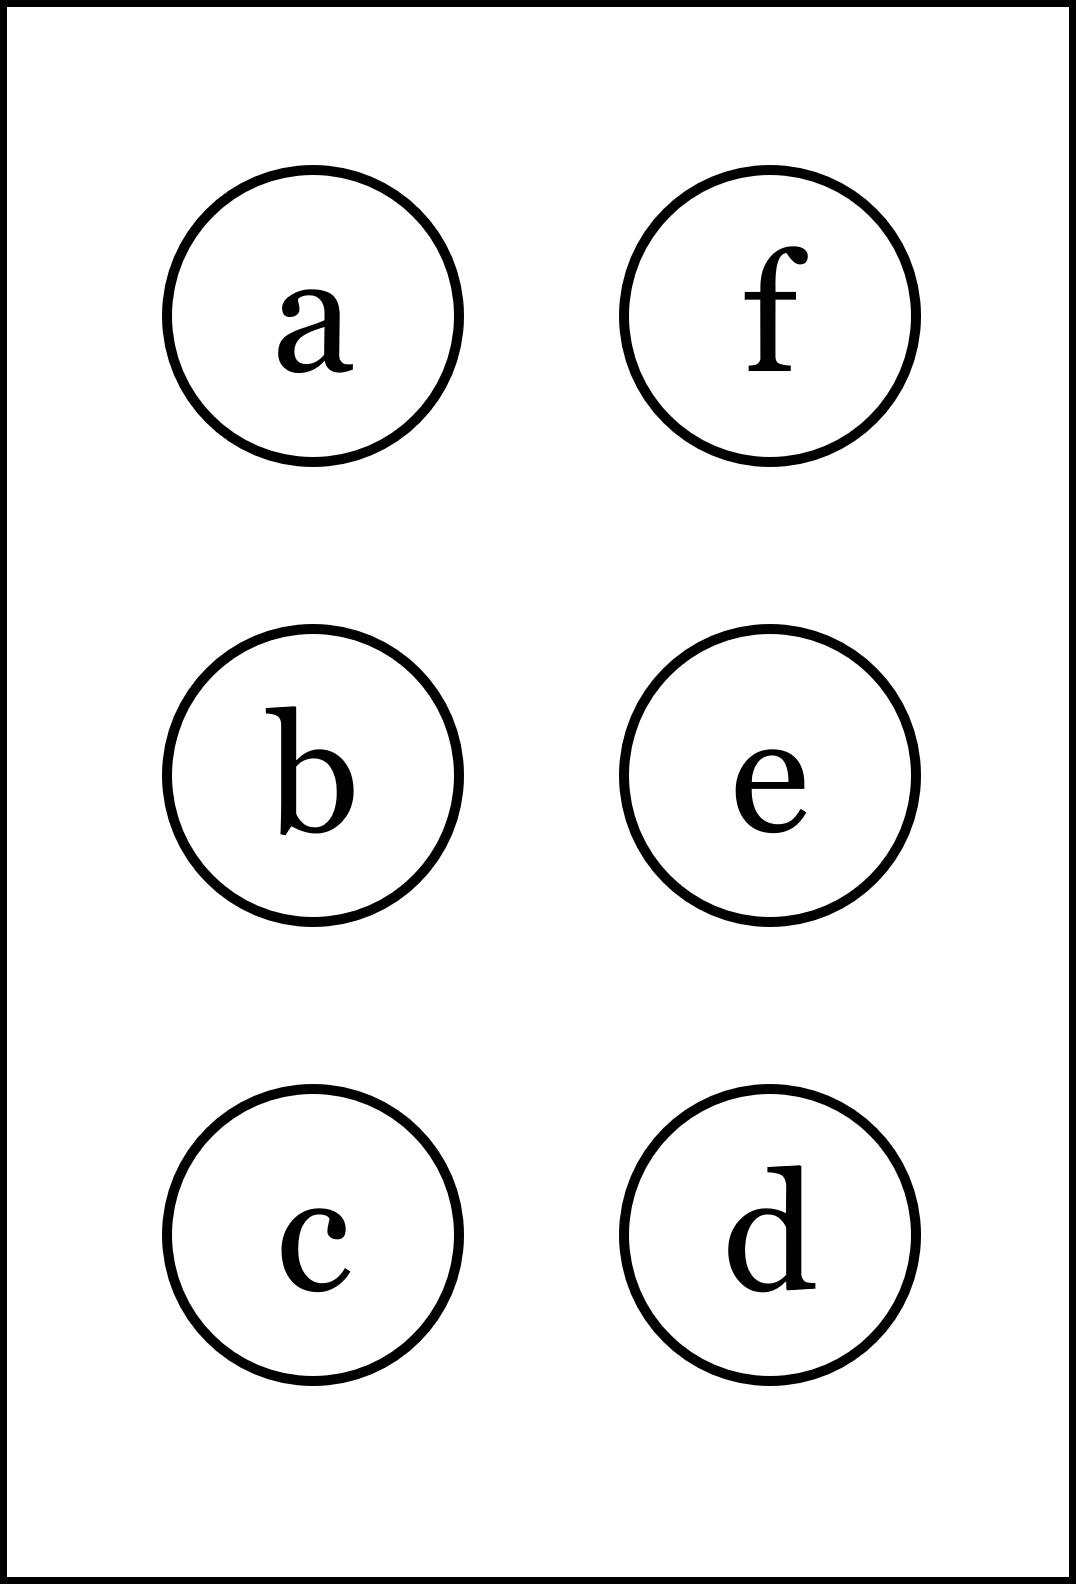
\includegraphics[height=40mm]{../images/braille.png}
{\small Písmeno Braillovej abecedy}
\end{center}
\end{minipage}
\end{center}
\end{minipage}
%
\end{tabular}
\newpage
\thispagestyle{empty}
\begin{tabular}{c:c}
\begin{minipage}[c][104.5mm][t]{0.5\linewidth}
\begin{center}
\vspace{7mm}
{\huge Stacionární body, skupina \textit{Delta $\delta$} -\romannumeral1}\\[5mm]
\textit{Jméno:}\phantom{xxxxxxxxxxxxxxxxxxxxxxxxxxxxxxxxxxxxxxxxxxxxxxxxxxxxxxxxxxxxxxxxx}\\[5mm]
\begin{minipage}{0.95\linewidth}
\begin{center}
{\small V \textbf{(a)} zjisti jestli $f(x)$ \textbf{roste} v bode $x_0$. V \textbf{(b)} zjisti jestli je $f(x)$ v bode $x_0$ \textbf{ryze konvexní}.\\V \textbf{(c)} spočti \textbf{součet} x-ových souřadnic stacionárního a inflexního bodu. V \textbf{(d)} najdi x-ovou souřadnici stacionárního bodu a rozhodli jestli to je \textbf{lomax, lomin či inflex}.\\Pokud se výsledky shodujú s těmi za otazníky, tak napravo obarvi příslušející kroužek načerno.\\\textbf{Spolu odevzdejte výsledné slovo}}.
\end{center}
\end{minipage}
\\[1mm]
\begin{minipage}{0.79\linewidth}
\begin{center}
\begin{varwidth}{\linewidth}
\begin{enumerate}
\normalsize
\item $f(x)=\cfrac{-7x^2+8x-2}{6x+2}\enspace , \enspace x_0=-1$\quad \dotfill\; ???\;\dotfill \quad \text{ano}
\item $f(x)=2x^4+3x^3+5x^2-4x-1\enspace , \enspace x_0=2$\quad \dotfill\; ???\;\dotfill \quad \text{ano}
\item $f(x)=-5xe^{-3x}$\quad \dotfill\; ???\;\dotfill \quad $1$
\item $f(x)=\sqrt{2x^2-x+2}$\quad \dotfill\; ???\;\dotfill \quad $\nicefrac{1}{4}\enspace , \enspace \mathrm{lomin}$
\item \quad \dotfill\; ???\;\dotfill \quad nebarvi
\item \quad \dotfill\; ???\;\dotfill \quad nebarvi
\end{enumerate}
\end{varwidth}
\end{center}
\end{minipage}
\begin{minipage}{0.20\linewidth}
\begin{center}
{\Huge\bfseries 1.} \\[2mm]
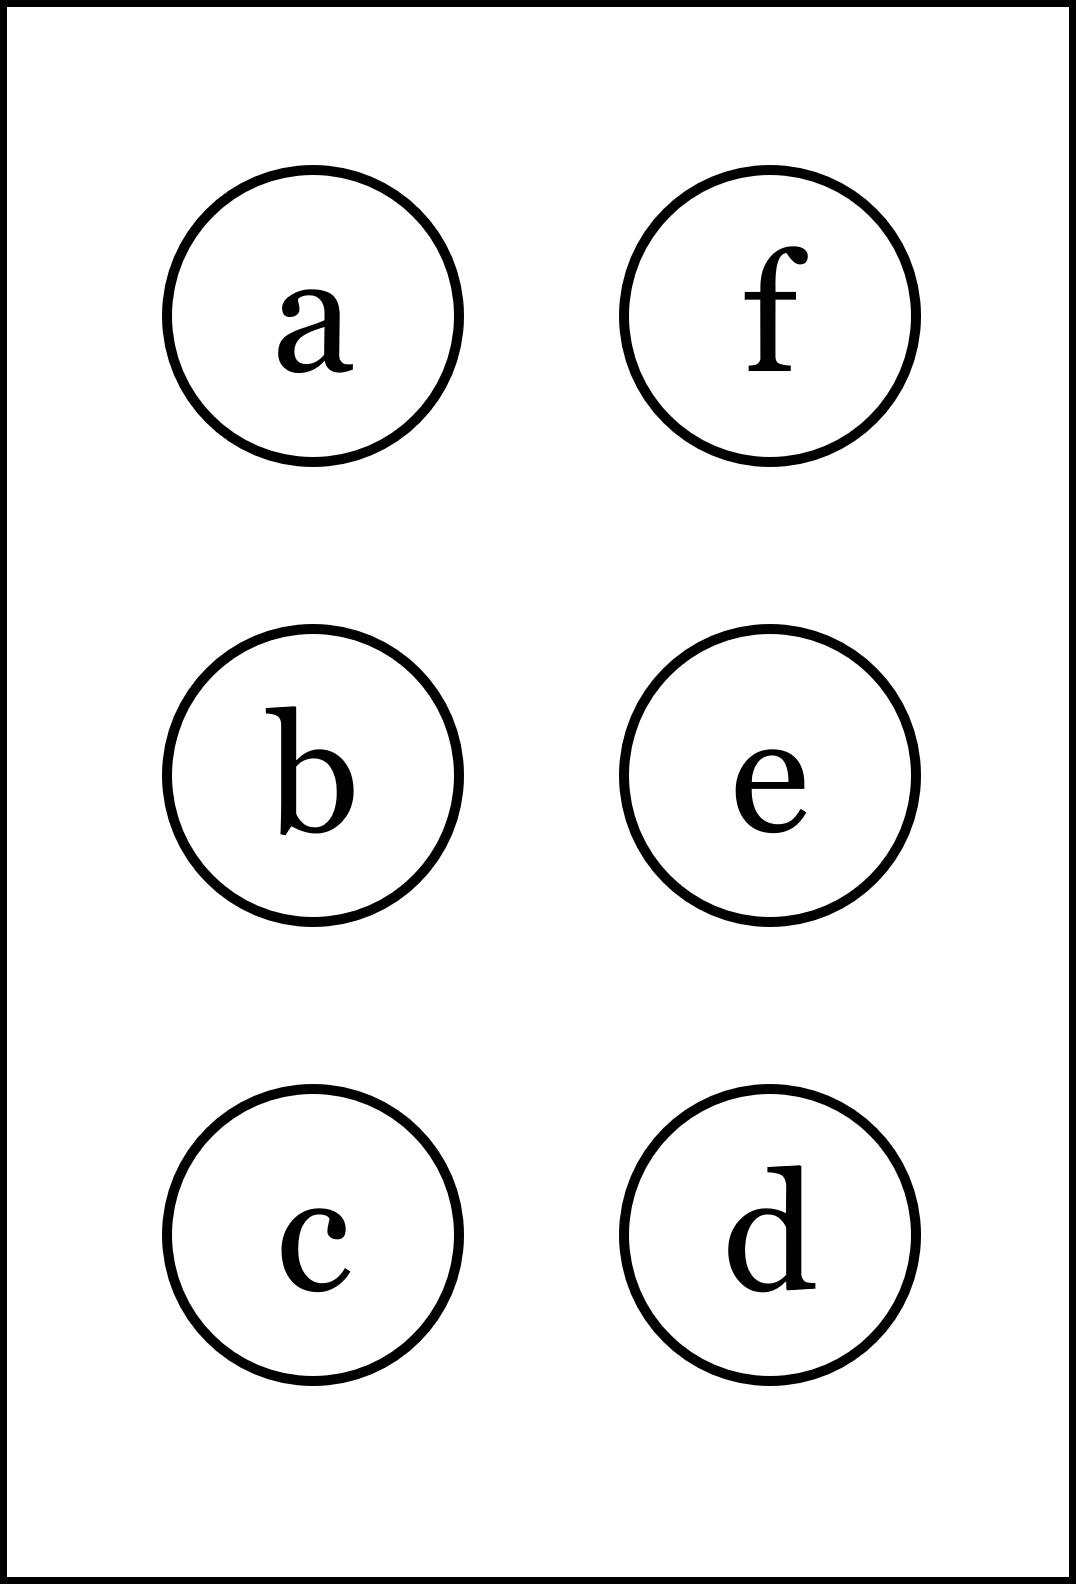
\includegraphics[height=40mm]{../images/braille.png}
{\small Písmeno Braillovej abecedy}
\end{center}
\end{minipage}
\end{center}
\end{minipage}
&
\begin{minipage}[c][104.5mm][t]{0.5\linewidth}
\begin{center}
\vspace{7mm}
{\huge Stacionární body, skupina \textit{Delta $\delta$} -\romannumeral2}\\[5mm]
\textit{Jméno:}\phantom{xxxxxxxxxxxxxxxxxxxxxxxxxxxxxxxxxxxxxxxxxxxxxxxxxxxxxxxxxxxxxxxxx}\\[5mm]
\begin{minipage}{0.95\linewidth}
\begin{center}
{\small V \textbf{(a)} zjisti jestli $f(x)$ \textbf{roste} v bode $x_0$. V \textbf{(b)} zjisti jestli je $f(x)$ v bode $x_0$ \textbf{ryze konvexní}.\\V \textbf{(c)} spočti \textbf{součet} x-ových souřadnic stacionárního a inflexního bodu. V \textbf{(d)} najdi x-ovou souřadnici stacionárního bodu a rozhodli jestli to je \textbf{lomax, lomin či inflex}.\\Pokud se výsledky shodujú s těmi za otazníky, tak napravo obarvi příslušející kroužek načerno.\\\textbf{Spolu odevzdejte výsledné slovo}}.
\end{center}
\end{minipage}
\\[1mm]
\begin{minipage}{0.79\linewidth}
\begin{center}
\begin{varwidth}{\linewidth}
\begin{enumerate}
\normalsize
\item $f(x)=\cfrac{5x^2+5x-1}{3x-2}\enspace , \enspace x_0=2$\quad \dotfill\; ???\;\dotfill \quad \text{ano}
\item $f(x)=4x^4+5x^3+6x^2+x-4\enspace , \enspace x_0=-1$\quad \dotfill\; ???\;\dotfill \quad \text{ne}
\item $f(x)=6xe^{-x}$\quad \dotfill\; ???\;\dotfill \quad $-1$
\item $f(x)=\sqrt{3x^2-3x+2}$\quad \dotfill\; ???\;\dotfill \quad $\nicefrac{1}{2}\enspace , \enspace\mathrm{lomax}$
\item \quad \dotfill\; ???\;\dotfill \quad nebarvi
\item \quad \dotfill\; ???\;\dotfill \quad nebarvi
\end{enumerate}
\end{varwidth}
\end{center}
\end{minipage}
\begin{minipage}{0.20\linewidth}
\begin{center}
{\Huge\bfseries 2.} \\[2mm]
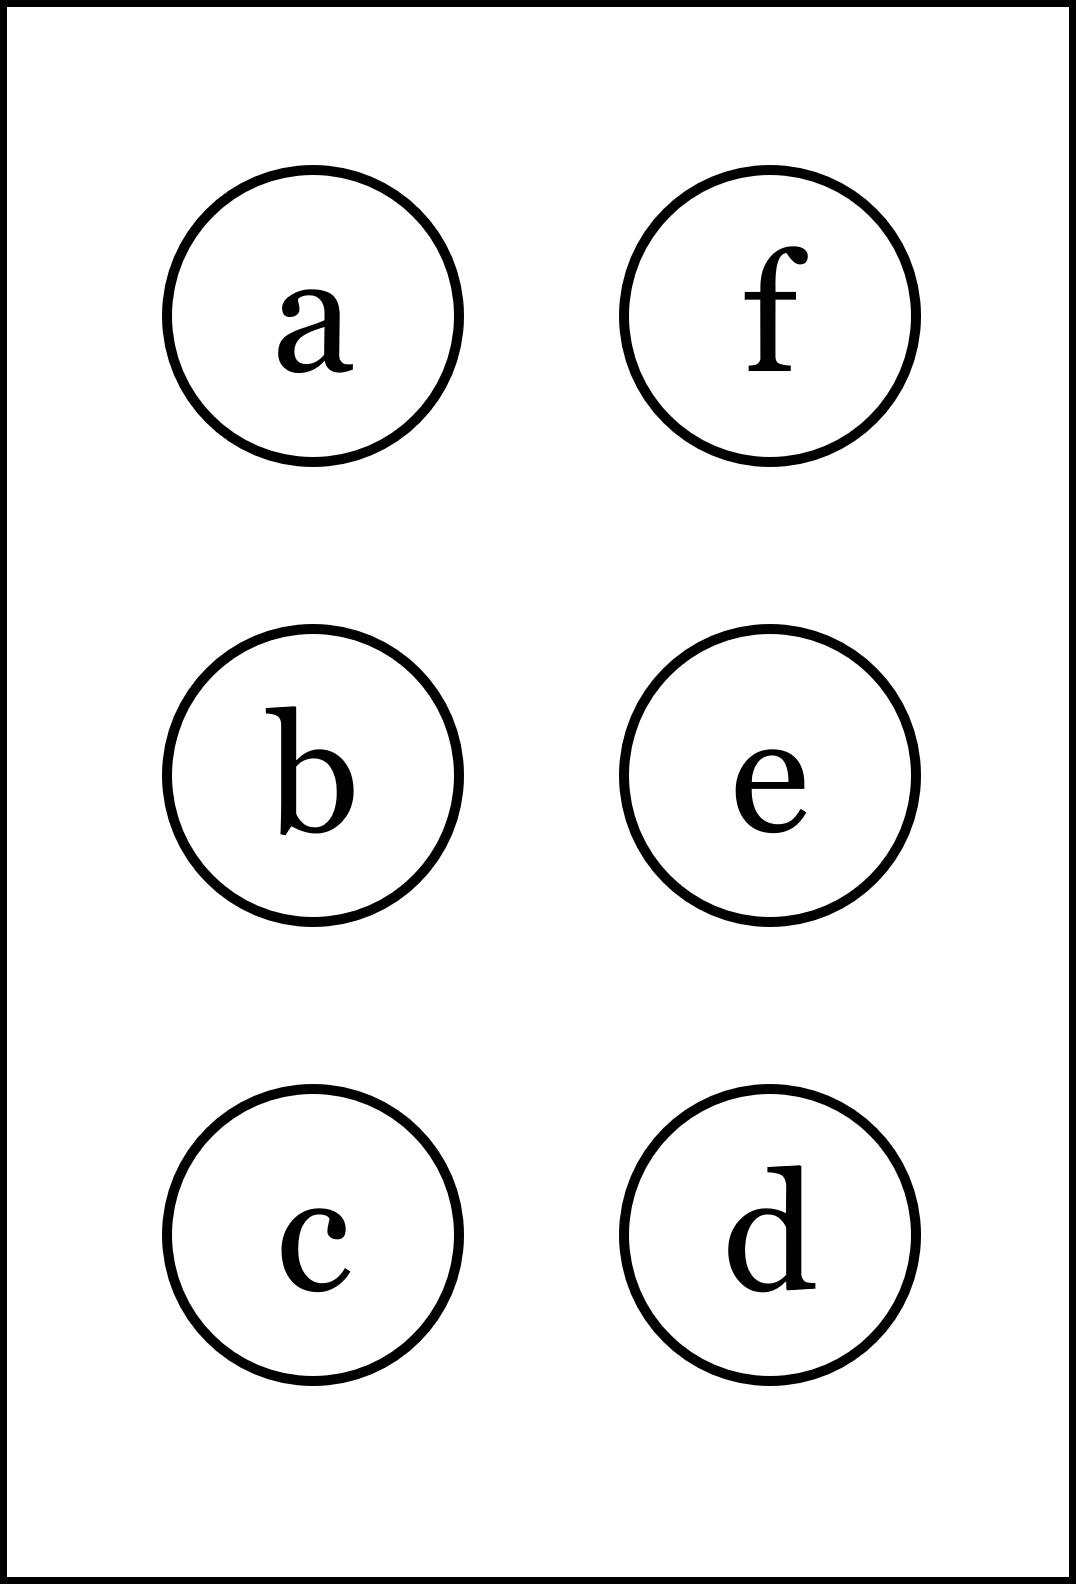
\includegraphics[height=40mm]{../images/braille.png}
{\small Písmeno Braillovej abecedy}
\end{center}
\end{minipage}
\end{center}
\end{minipage}
\\ \hdashline
\begin{minipage}[c][104.5mm][t]{0.5\linewidth}
\begin{center}
\vspace{7mm}
{\huge Stacionární body, skupina \textit{Delta $\delta$} -\romannumeral3}\\[5mm]
\textit{Jméno:}\phantom{xxxxxxxxxxxxxxxxxxxxxxxxxxxxxxxxxxxxxxxxxxxxxxxxxxxxxxxxxxxxxxxxx}\\[5mm]
\begin{minipage}{0.95\linewidth}
\begin{center}
{\small V \textbf{(a)} zjisti jestli $f(x)$ \textbf{roste} v bode $x_0$. V \textbf{(b)} zjisti jestli je $f(x)$ v bode $x_0$ \textbf{ryze konvexní}.\\V \textbf{(c)} spočti \textbf{součet} x-ových souřadnic stacionárního a inflexního bodu. V \textbf{(d)} najdi x-ovou souřadnici stacionárního bodu a rozhodli jestli to je \textbf{lomax, lomin či inflex}.\\Pokud se výsledky shodujú s těmi za otazníky, tak napravo obarvi příslušející kroužek načerno.\\\textbf{Spolu odevzdejte výsledné slovo}}.
\end{center}
\end{minipage}
\\[1mm]
\begin{minipage}{0.79\linewidth}
\begin{center}
\begin{varwidth}{\linewidth}
\begin{enumerate}
\normalsize
\item $f(x)=\cfrac{-x^2+x-2}{7x-4}\enspace , \enspace x_0=-1$\quad \dotfill\; ???\;\dotfill \quad \text{ne}
\item $f(x)=9x^4+9x^3+x^2-4x+1\enspace , \enspace x_0=2$\quad \dotfill\; ???\;\dotfill \quad \text{ne}
\item $f(x)=-xe^{6x}$\quad \dotfill\; ???\;\dotfill \quad $\nicefrac{-1}{2}$
\item $f(x)=\sqrt{4x^2+x+2}$\quad \dotfill\; ???\;\dotfill \quad $\nicefrac{-1}{8}\enspace , \enspace\mathrm{inflex}$
\item \quad \dotfill\; ???\;\dotfill \quad vybarvi
\item \quad \dotfill\; ???\;\dotfill \quad vybarvi
\end{enumerate}
\end{varwidth}
\end{center}
\end{minipage}
\begin{minipage}{0.20\linewidth}
\begin{center}
{\Huge\bfseries 3.} \\[2mm]
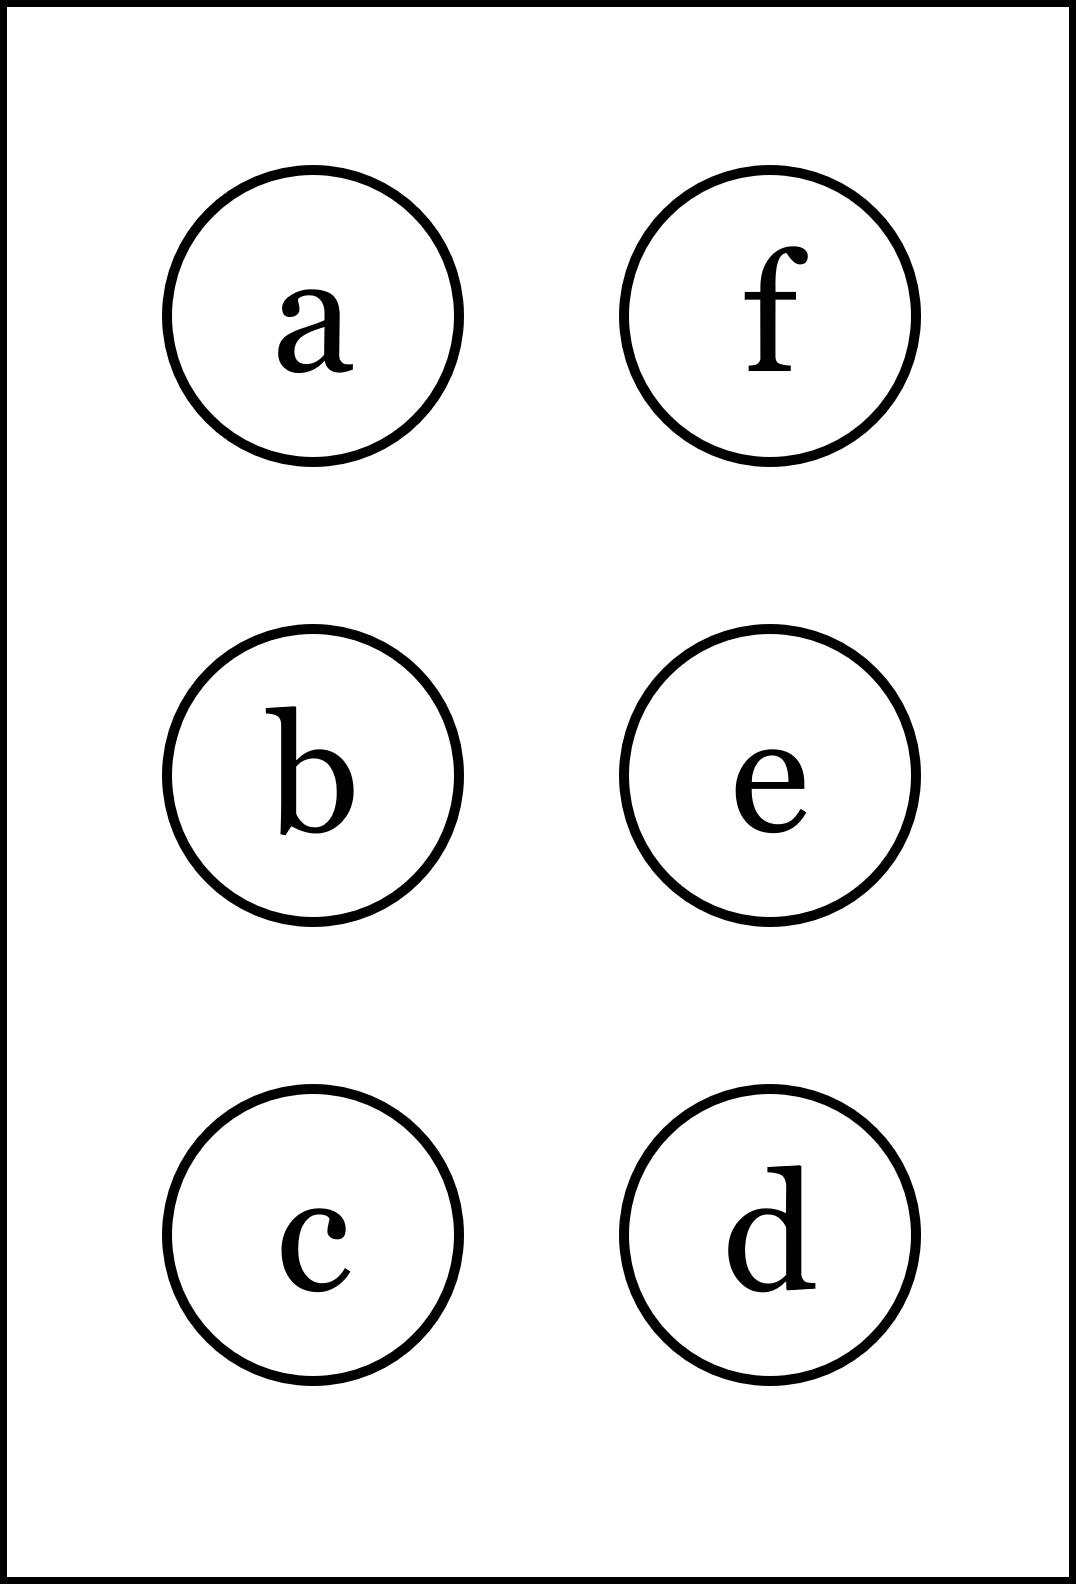
\includegraphics[height=40mm]{../images/braille.png}
{\small Písmeno Braillovej abecedy}
\end{center}
\end{minipage}
\end{center}
\end{minipage}
&
\begin{minipage}[c][104.5mm][t]{0.5\linewidth}
\begin{center}
\vspace{7mm}
{\huge Stacionární body, skupina \textit{Delta $\delta$} -\romannumeral4}\\[5mm]
\textit{Jméno:}\phantom{xxxxxxxxxxxxxxxxxxxxxxxxxxxxxxxxxxxxxxxxxxxxxxxxxxxxxxxxxxxxxxxxx}\\[5mm]
\begin{minipage}{0.95\linewidth}
\begin{center}
{\small V \textbf{(a)} zjisti jestli $f(x)$ \textbf{roste} v bode $x_0$. V \textbf{(b)} zjisti jestli je $f(x)$ v bode $x_0$ \textbf{ryze konvexní}.\\V \textbf{(c)} spočti \textbf{součet} x-ových souřadnic stacionárního a inflexního bodu. V \textbf{(d)} najdi x-ovou souřadnici stacionárního bodu a rozhodli jestli to je \textbf{lomax, lomin či inflex}.\\Pokud se výsledky shodujú s těmi za otazníky, tak napravo obarvi příslušející kroužek načerno.\\\textbf{Spolu odevzdejte výsledné slovo}}.
\end{center}
\end{minipage}
\\[1mm]
\begin{minipage}{0.79\linewidth}
\begin{center}
\begin{varwidth}{\linewidth}
\begin{enumerate}
\normalsize
\item $f(x)=\cfrac{-x^2+3x-5}{-x+1}\enspace , \enspace x_0=-4$\quad \dotfill\; ???\;\dotfill \quad \text{ano}
\item $f(x)=x^4+2x^3-x^2+x-1\enspace , \enspace x_0=2$\quad \dotfill\; ???\;\dotfill \quad \text{ne}
\item $f(x)=2xe^{-6x}$\quad \dotfill\; ???\;\dotfill \quad $\nicefrac{-1}{6}$
\item $f(x)=\sqrt{x^2+2x+5}$\quad \dotfill\; ???\;\dotfill \quad $-1\enspace , \enspace\mathrm{lomax}$
\item \quad \dotfill\; ???\;\dotfill \quad nebarvi
\item \quad \dotfill\; ???\;\dotfill \quad nebarvi
\end{enumerate}
\end{varwidth}
\end{center}
\end{minipage}
\begin{minipage}{0.20\linewidth}
\begin{center}
{\Huge\bfseries 4.} \\[2mm]
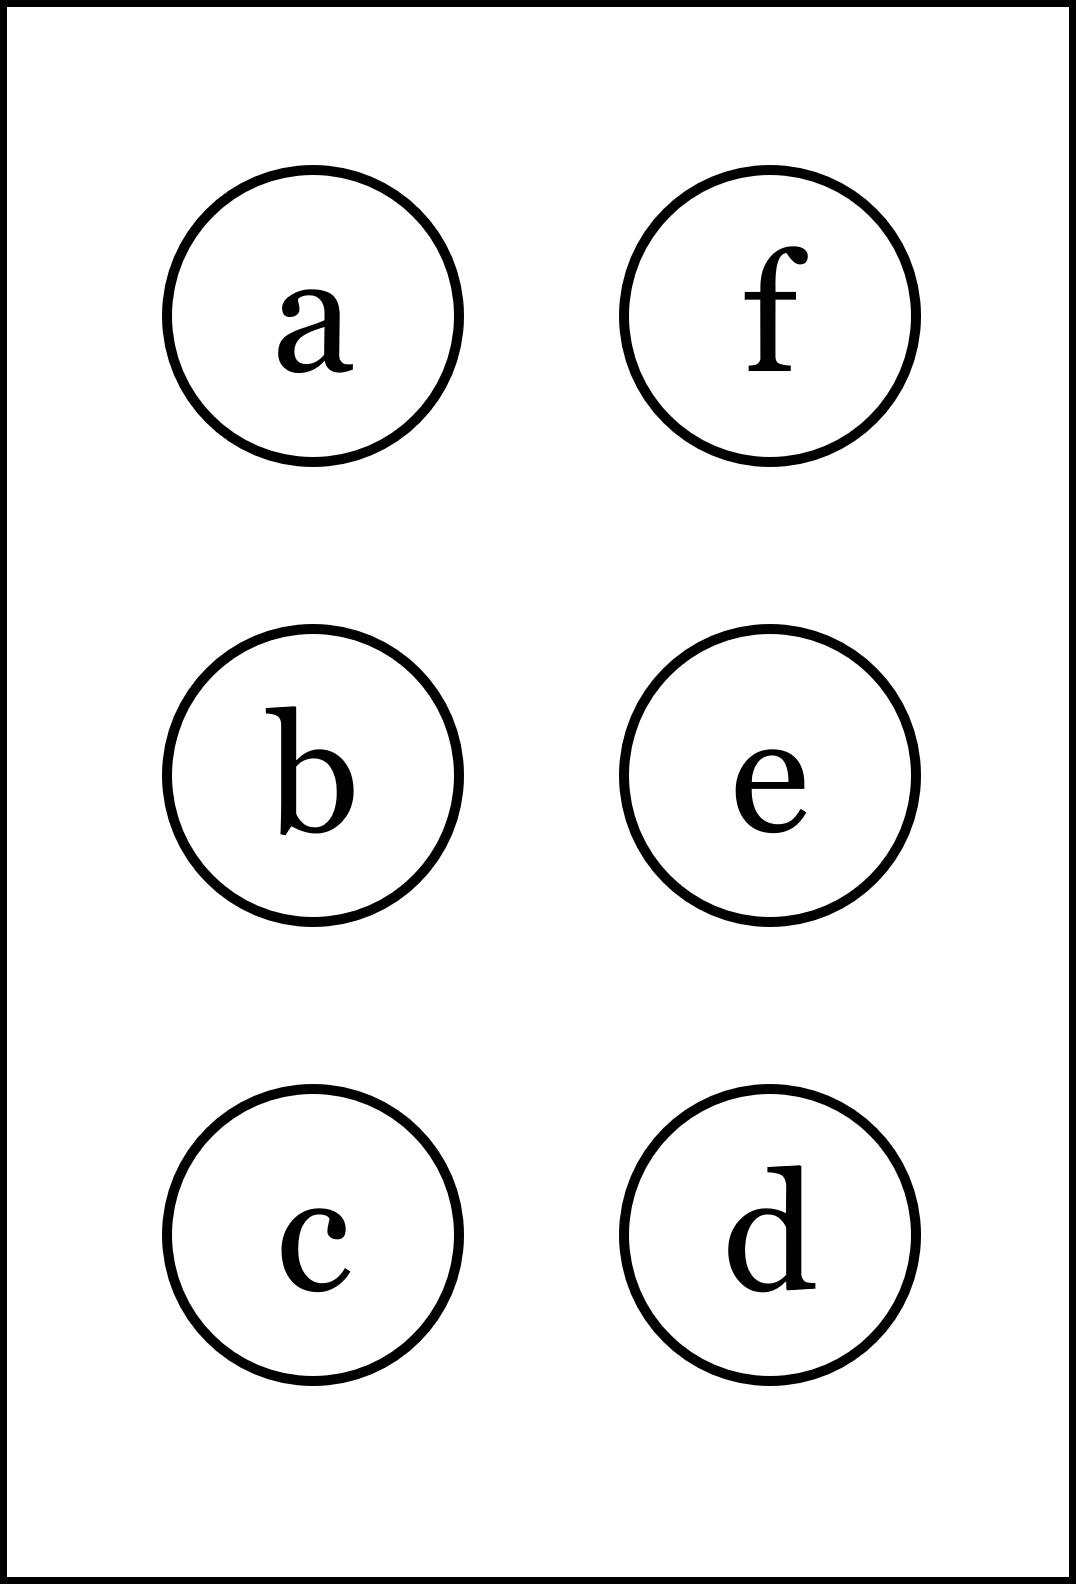
\includegraphics[height=40mm]{../images/braille.png}
{\small Písmeno Braillovej abecedy}
\end{center}
\end{minipage}
\end{center}
\end{minipage}
%
\end{tabular}
\newpage
\thispagestyle{empty}
\begin{tabular}{c:c}
\begin{minipage}[c][104.5mm][t]{0.5\linewidth}
\begin{center}
\vspace{7mm}
{\huge Stacionární body, skupina \textit{Epsilon $\epsilon$} -\romannumeral1}\\[5mm]
\textit{Jméno:}\phantom{xxxxxxxxxxxxxxxxxxxxxxxxxxxxxxxxxxxxxxxxxxxxxxxxxxxxxxxxxxxxxxxxx}\\[5mm]
\begin{minipage}{0.95\linewidth}
\begin{center}
{\small V \textbf{(a)} zjisti jestli $f(x)$ \textbf{roste} v bode $x_0$. V \textbf{(b)} zjisti jestli je $f(x)$ v bode $x_0$ \textbf{ryze konvexní}.\\V \textbf{(c)} spočti \textbf{součet} x-ových souřadnic stacionárního a inflexního bodu. V \textbf{(d)} najdi x-ovou souřadnici stacionárního bodu a rozhodli jestli to je \textbf{lomax, lomin či inflex}.\\Pokud se výsledky shodujú s těmi za otazníky, tak napravo obarvi příslušející kroužek načerno.\\\textbf{Spolu odevzdejte výsledné slovo}}.
\end{center}
\end{minipage}
\\[1mm]
\begin{minipage}{0.79\linewidth}
\begin{center}
\begin{varwidth}{\linewidth}
\begin{enumerate}
\normalsize
\item $f(x)=\cfrac{3x^2+9x+1}{-6x-6}\enspace , \enspace x_0=2$\quad \dotfill\; ???\;\dotfill \quad \text{ano}
\item $f(x)=3x^4+8x^3-5x^2-4x-4\enspace , \enspace x_0=-3$\quad \dotfill\; ???\;\dotfill \quad \text{ano}
\item $f(x)=-7xe^{-8x}$\quad \dotfill\; ???\;\dotfill \quad $\nicefrac{-1}{8}$
\item $f(x)=\sqrt{2x^2-2x+1}$\quad \dotfill\; ???\;\dotfill \quad $\nicefrac{1}{2}\enspace , \enspace\mathrm{lomax}$
\item \quad \dotfill\; ???\;\dotfill \quad nebarvi
\item \quad \dotfill\; ???\;\dotfill \quad vybarvi
\end{enumerate}
\end{varwidth}
\end{center}
\end{minipage}
\begin{minipage}{0.20\linewidth}
\begin{center}
{\Huge\bfseries 1.} \\[2mm]
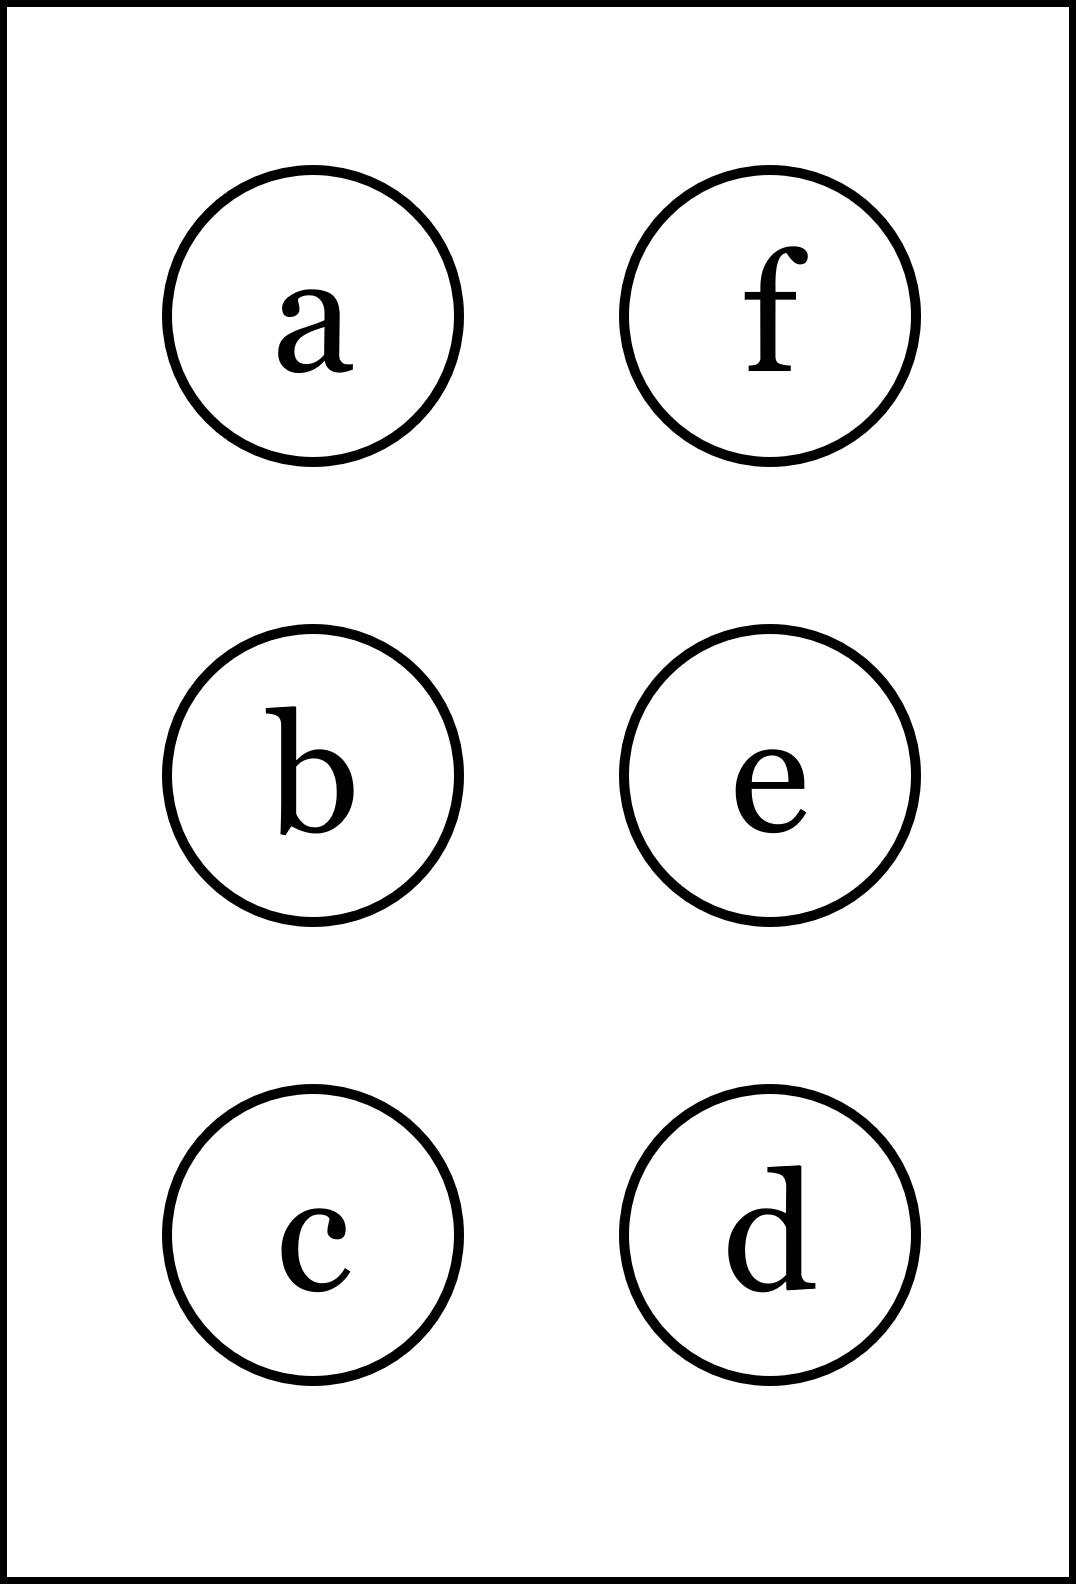
\includegraphics[height=40mm]{../images/braille.png}
{\small Písmeno Braillovej abecedy}
\end{center}
\end{minipage}
\end{center}
\end{minipage}
&
\begin{minipage}[c][104.5mm][t]{0.5\linewidth}
\begin{center}
\vspace{7mm}
{\huge Stacionární body, skupina \textit{Epsilon $\epsilon$} -\romannumeral2}\\[5mm]
\textit{Jméno:}\phantom{xxxxxxxxxxxxxxxxxxxxxxxxxxxxxxxxxxxxxxxxxxxxxxxxxxxxxxxxxxxxxxxxx}\\[5mm]
\begin{minipage}{0.95\linewidth}
\begin{center}
{\small V \textbf{(a)} zjisti jestli $f(x)$ \textbf{roste} v bode $x_0$. V \textbf{(b)} zjisti jestli je $f(x)$ v bode $x_0$ \textbf{ryze konvexní}.\\V \textbf{(c)} spočti \textbf{součet} x-ových souřadnic stacionárního a inflexního bodu. V \textbf{(d)} najdi x-ovou souřadnici stacionárního bodu a rozhodli jestli to je \textbf{lomax, lomin či inflex}.\\Pokud se výsledky shodujú s těmi za otazníky, tak napravo obarvi příslušející kroužek načerno.\\\textbf{Spolu odevzdejte výsledné slovo}}.
\end{center}
\end{minipage}
\\[1mm]
\begin{minipage}{0.79\linewidth}
\begin{center}
\begin{varwidth}{\linewidth}
\begin{enumerate}
\normalsize
\item $f(x)=\cfrac{7x^2-4x+7}{x-2}\enspace , \enspace x_0=-2$\quad \dotfill\; ???\;\dotfill \quad \text{ano}
\item $f(x)=-3x^4+2x^3-x^2-3x+4\enspace , \enspace x_0=-1$\quad \dotfill\; ???\;\dotfill \quad \text{ne}
\item $f(x)=-2xe^{-x}$\quad \dotfill\; ???\;\dotfill \quad $3$
\item $f(x)=\sqrt{4x^2-4x+4}$\quad \dotfill\; ???\;\dotfill \quad $\nicefrac{1}{2}\enspace , \enspace \mathrm{lomin}$
\item \quad \dotfill\; ???\;\dotfill \quad nebarvi
\item \quad \dotfill\; ???\;\dotfill \quad nebarvi
\end{enumerate}
\end{varwidth}
\end{center}
\end{minipage}
\begin{minipage}{0.20\linewidth}
\begin{center}
{\Huge\bfseries 2.} \\[2mm]
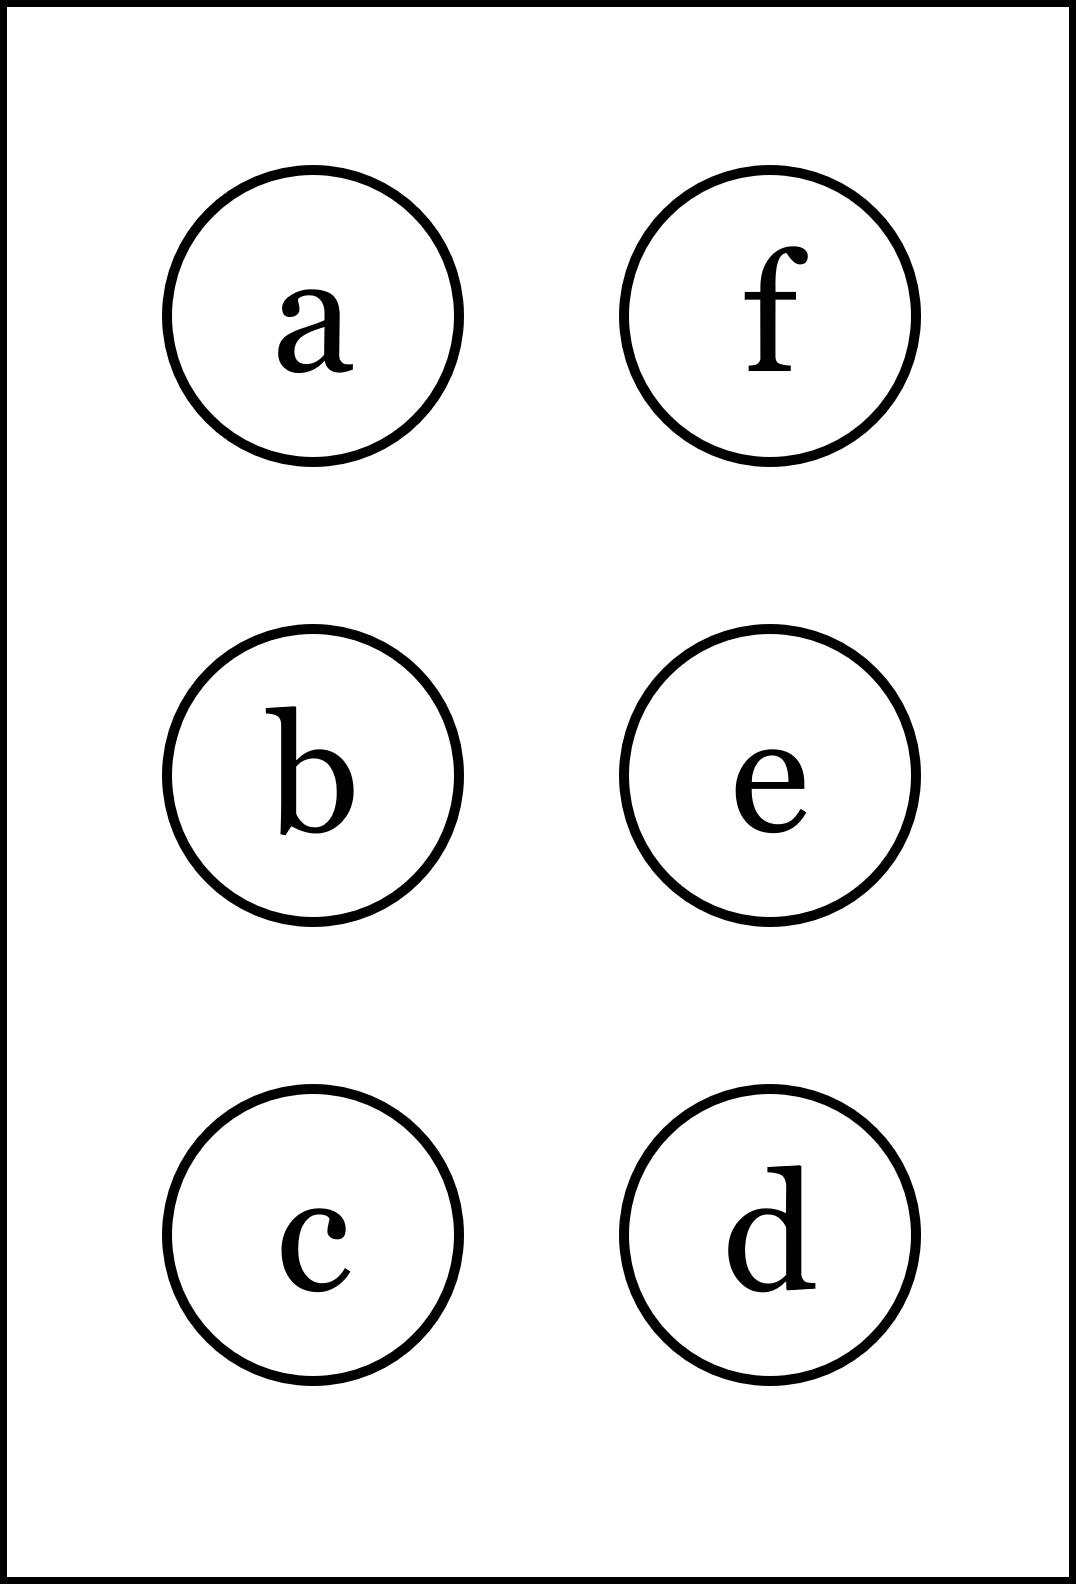
\includegraphics[height=40mm]{../images/braille.png}
{\small Písmeno Braillovej abecedy}
\end{center}
\end{minipage}
\end{center}
\end{minipage}
\\ \hdashline
\begin{minipage}[c][104.5mm][t]{0.5\linewidth}
\begin{center}
\vspace{7mm}
{\huge Stacionární body, skupina \textit{Epsilon $\epsilon$} -\romannumeral3}\\[5mm]
\textit{Jméno:}\phantom{xxxxxxxxxxxxxxxxxxxxxxxxxxxxxxxxxxxxxxxxxxxxxxxxxxxxxxxxxxxxxxxxx}\\[5mm]
\begin{minipage}{0.95\linewidth}
\begin{center}
{\small V \textbf{(a)} zjisti jestli $f(x)$ \textbf{roste} v bode $x_0$. V \textbf{(b)} zjisti jestli je $f(x)$ v bode $x_0$ \textbf{ryze konvexní}.\\V \textbf{(c)} spočti \textbf{součet} x-ových souřadnic stacionárního a inflexního bodu. V \textbf{(d)} najdi x-ovou souřadnici stacionárního bodu a rozhodli jestli to je \textbf{lomax, lomin či inflex}.\\Pokud se výsledky shodujú s těmi za otazníky, tak napravo obarvi příslušející kroužek načerno.\\\textbf{Spolu odevzdejte výsledné slovo}}.
\end{center}
\end{minipage}
\\[1mm]
\begin{minipage}{0.79\linewidth}
\begin{center}
\begin{varwidth}{\linewidth}
\begin{enumerate}
\normalsize
\item $f(x)=\cfrac{x^2+2x+3}{6x+6}\enspace , \enspace x_0=2$\quad \dotfill\; ???\;\dotfill \quad \text{ano}
\item $f(x)=-2x^4-x^3+x^2-7x-4\enspace , \enspace x_0=-2$\quad \dotfill\; ???\;\dotfill \quad \text{ano}
\item $f(x)=xe^{-8x}$\quad \dotfill\; ???\;\dotfill \quad $\nicefrac{-1}{8}$
\item $f(x)=\sqrt{4x^2-2x+4}$\quad \dotfill\; ???\;\dotfill \quad $\nicefrac{1}{4}\enspace , \enspace\mathrm{lomax}$
\item \quad \dotfill\; ???\;\dotfill \quad nebarvi
\item \quad \dotfill\; ???\;\dotfill \quad nebarvi
\end{enumerate}
\end{varwidth}
\end{center}
\end{minipage}
\begin{minipage}{0.20\linewidth}
\begin{center}
{\Huge\bfseries 3.} \\[2mm]
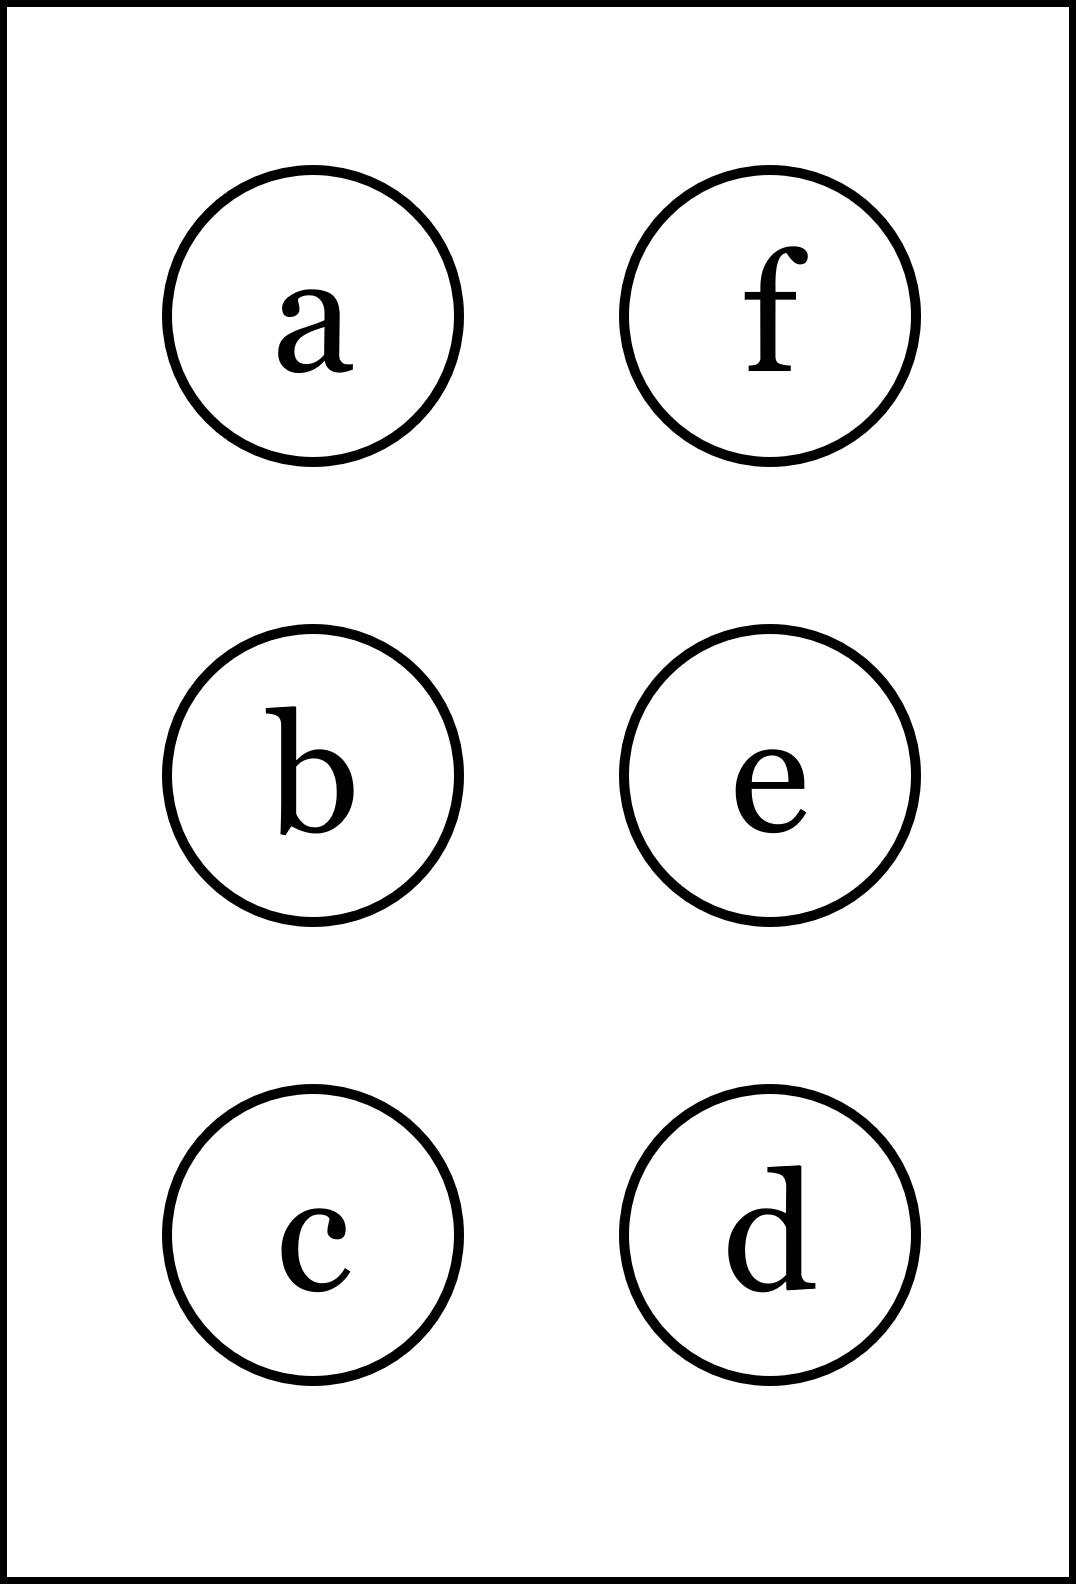
\includegraphics[height=40mm]{../images/braille.png}
{\small Písmeno Braillovej abecedy}
\end{center}
\end{minipage}
\end{center}
\end{minipage}
&
\begin{minipage}[c][104.5mm][t]{0.5\linewidth}
\begin{center}
\vspace{7mm}
{\huge Stacionární body, skupina \textit{Epsilon $\epsilon$} -\romannumeral4}\\[5mm]
\textit{Jméno:}\phantom{xxxxxxxxxxxxxxxxxxxxxxxxxxxxxxxxxxxxxxxxxxxxxxxxxxxxxxxxxxxxxxxxx}\\[5mm]
\begin{minipage}{0.95\linewidth}
\begin{center}
{\small V \textbf{(a)} zjisti jestli $f(x)$ \textbf{roste} v bode $x_0$. V \textbf{(b)} zjisti jestli je $f(x)$ v bode $x_0$ \textbf{ryze konvexní}.\\V \textbf{(c)} spočti \textbf{součet} x-ových souřadnic stacionárního a inflexního bodu. V \textbf{(d)} najdi x-ovou souřadnici stacionárního bodu a rozhodli jestli to je \textbf{lomax, lomin či inflex}.\\Pokud se výsledky shodujú s těmi za otazníky, tak napravo obarvi příslušející kroužek načerno.\\\textbf{Spolu odevzdejte výsledné slovo}}.
\end{center}
\end{minipage}
\\[1mm]
\begin{minipage}{0.79\linewidth}
\begin{center}
\begin{varwidth}{\linewidth}
\begin{enumerate}
\normalsize
\item $f(x)=\cfrac{3x^2+5x-5}{2x+8}\enspace , \enspace x_0=3$\quad \dotfill\; ???\;\dotfill \quad \text{ano}
\item $f(x)=6x^4-x^3+4x^2-x+7\enspace , \enspace x_0=-2$\quad \dotfill\; ???\;\dotfill \quad \text{ne}
\item $f(x)=-9xe^{-8x}$\quad \dotfill\; ???\;\dotfill \quad $\nicefrac{3}{8}$
\item $f(x)=\sqrt{2x^2-2x+4}$\quad \dotfill\; ???\;\dotfill \quad $\nicefrac{1}{2}\enspace , \enspace\mathrm{lomax}$
\item \quad \dotfill\; ???\;\dotfill \quad vybarvi
\item \quad \dotfill\; ???\;\dotfill \quad vybarvi
\end{enumerate}
\end{varwidth}
\end{center}
\end{minipage}
\begin{minipage}{0.20\linewidth}
\begin{center}
{\Huge\bfseries 4.} \\[2mm]
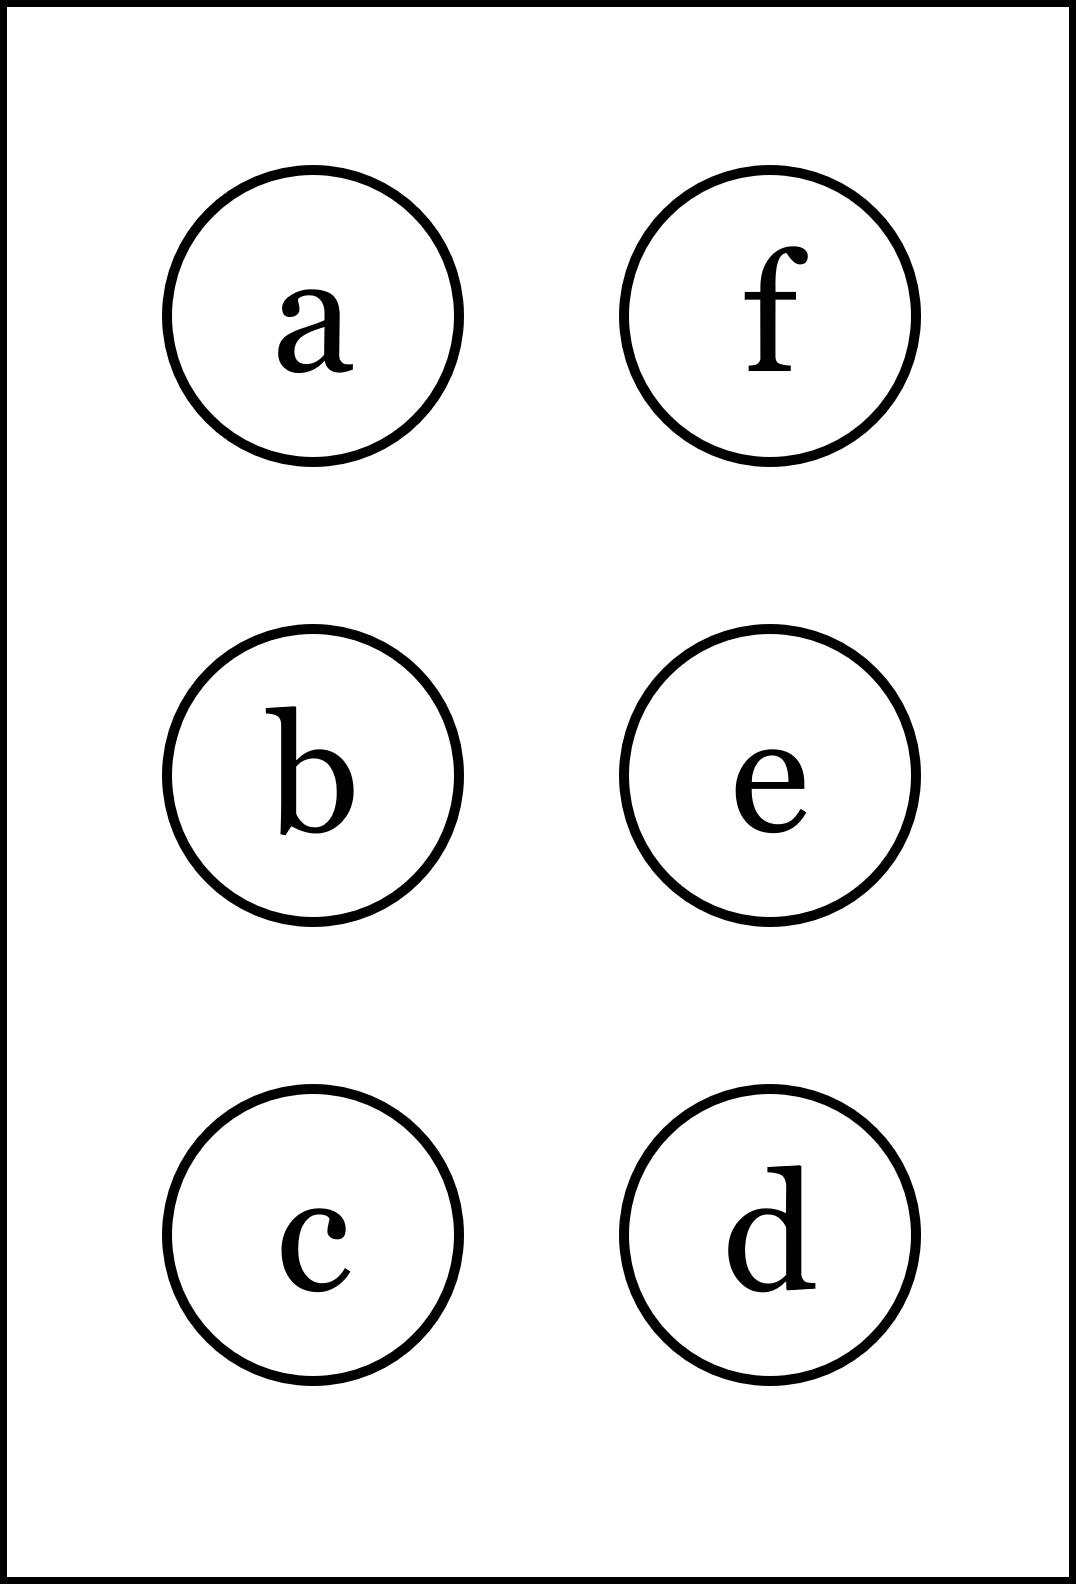
\includegraphics[height=40mm]{../images/braille.png}
{\small Písmeno Braillovej abecedy}
\end{center}
\end{minipage}
\end{center}
\end{minipage}
%
\end{tabular}
\newpage
\thispagestyle{empty}
\begin{tabular}{c:c}
\begin{minipage}[c][104.5mm][t]{0.5\linewidth}
\begin{center}
\vspace{7mm}
{\huge Stacionární body, skupina \textit{Zeta $\zeta$} -\romannumeral1}\\[5mm]
\textit{Jméno:}\phantom{xxxxxxxxxxxxxxxxxxxxxxxxxxxxxxxxxxxxxxxxxxxxxxxxxxxxxxxxxxxxxxxxx}\\[5mm]
\begin{minipage}{0.95\linewidth}
\begin{center}
{\small V \textbf{(a)} zjisti jestli $f(x)$ \textbf{roste} v bode $x_0$. V \textbf{(b)} zjisti jestli je $f(x)$ v bode $x_0$ \textbf{ryze konvexní}.\\V \textbf{(c)} spočti \textbf{součet} x-ových souřadnic stacionárního a inflexního bodu. V \textbf{(d)} najdi x-ovou souřadnici stacionárního bodu a rozhodli jestli to je \textbf{lomax, lomin či inflex}.\\Pokud se výsledky shodujú s těmi za otazníky, tak napravo obarvi příslušející kroužek načerno.\\\textbf{Spolu odevzdejte výsledné slovo}}.
\end{center}
\end{minipage}
\\[1mm]
\begin{minipage}{0.79\linewidth}
\begin{center}
\begin{varwidth}{\linewidth}
\begin{enumerate}
\normalsize
\item $f(x)=\cfrac{-3x^2-5x+2}{-5x-2}\enspace , \enspace x_0=-2$\quad \dotfill\; ???\;\dotfill \quad \text{ano}
\item $f(x)=-x^4+3x^3-6x^2+x-4\enspace , \enspace x_0=-1$\quad \dotfill\; ???\;\dotfill \quad \text{ne}
\item $f(x)=-3xe^{8x}$\quad \dotfill\; ???\;\dotfill \quad $\nicefrac{1}{8}$
\item $f(x)=\sqrt{5x^2-3x+4}$\quad \dotfill\; ???\;\dotfill \quad $\nicefrac{3}{10}\enspace , \enspace\mathrm{lomax}$
\item \quad \dotfill\; ???\;\dotfill \quad nebarvi
\item \quad \dotfill\; ???\;\dotfill \quad vybarvi
\end{enumerate}
\end{varwidth}
\end{center}
\end{minipage}
\begin{minipage}{0.20\linewidth}
\begin{center}
{\Huge\bfseries 1.} \\[2mm]
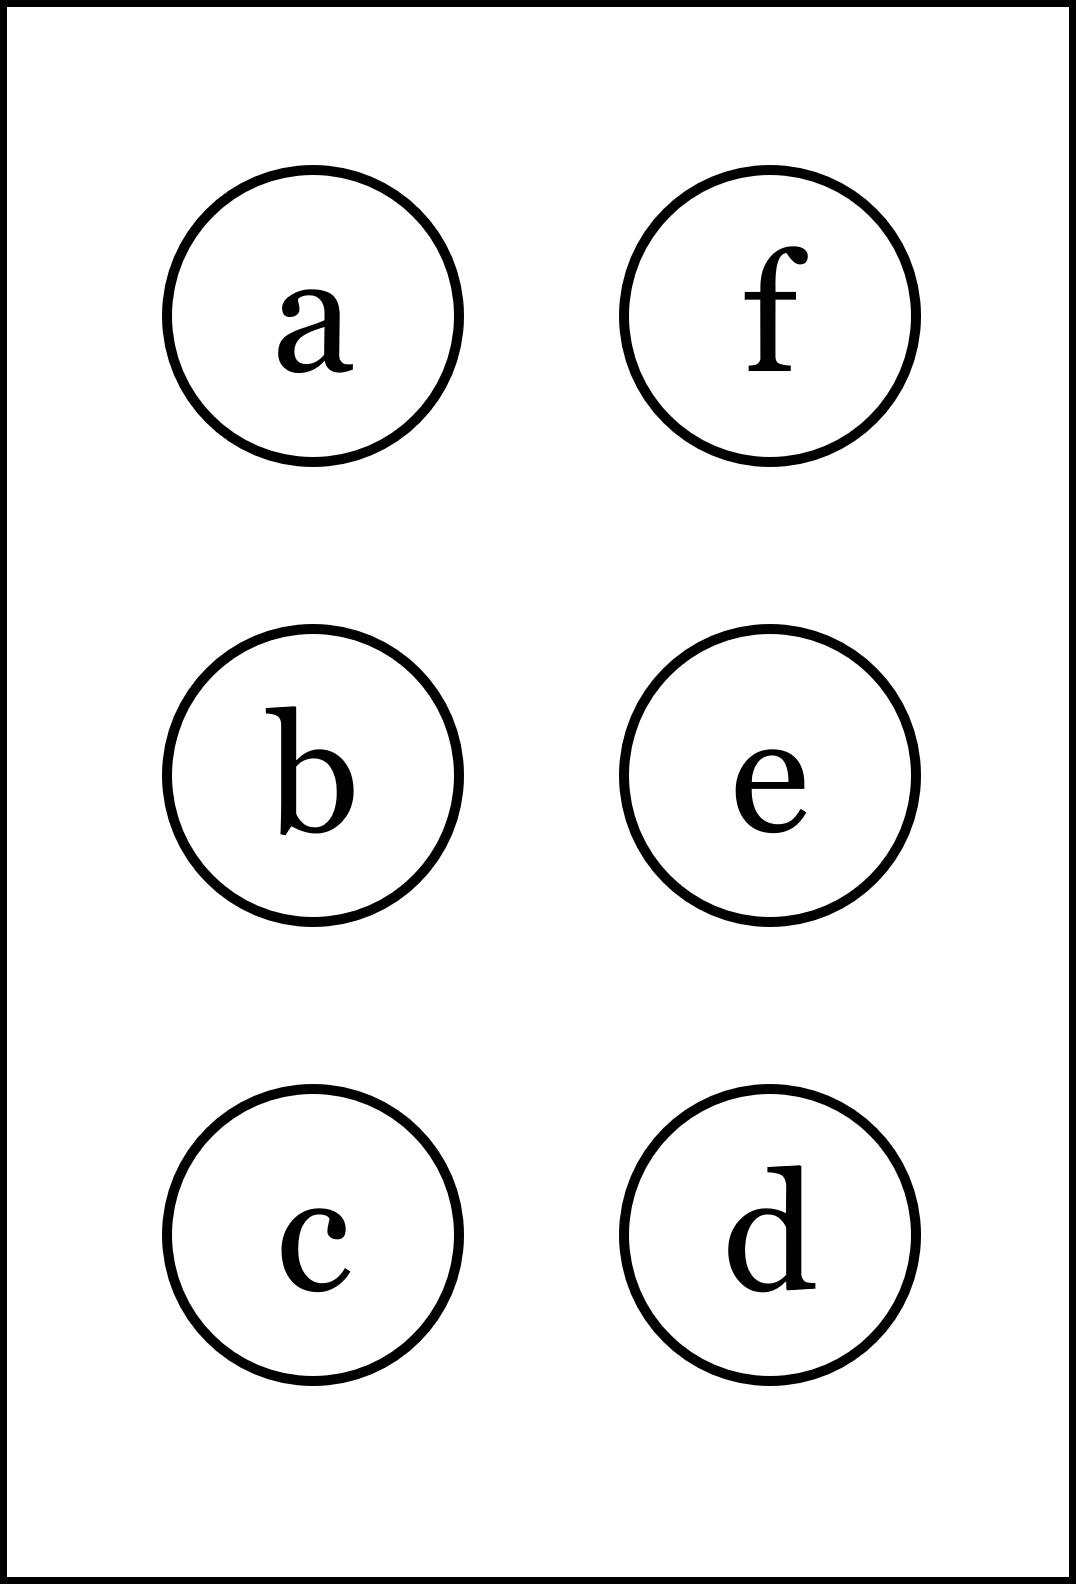
\includegraphics[height=40mm]{../images/braille.png}
{\small Písmeno Braillovej abecedy}
\end{center}
\end{minipage}
\end{center}
\end{minipage}
&
\begin{minipage}[c][104.5mm][t]{0.5\linewidth}
\begin{center}
\vspace{7mm}
{\huge Stacionární body, skupina \textit{Zeta $\zeta$} -\romannumeral2}\\[5mm]
\textit{Jméno:}\phantom{xxxxxxxxxxxxxxxxxxxxxxxxxxxxxxxxxxxxxxxxxxxxxxxxxxxxxxxxxxxxxxxxx}\\[5mm]
\begin{minipage}{0.95\linewidth}
\begin{center}
{\small V \textbf{(a)} zjisti jestli $f(x)$ \textbf{roste} v bode $x_0$. V \textbf{(b)} zjisti jestli je $f(x)$ v bode $x_0$ \textbf{ryze konvexní}.\\V \textbf{(c)} spočti \textbf{součet} x-ových souřadnic stacionárního a inflexního bodu. V \textbf{(d)} najdi x-ovou souřadnici stacionárního bodu a rozhodli jestli to je \textbf{lomax, lomin či inflex}.\\Pokud se výsledky shodujú s těmi za otazníky, tak napravo obarvi příslušející kroužek načerno.\\\textbf{Spolu odevzdejte výsledné slovo}}.
\end{center}
\end{minipage}
\\[1mm]
\begin{minipage}{0.79\linewidth}
\begin{center}
\begin{varwidth}{\linewidth}
\begin{enumerate}
\normalsize
\item $f(x)=\cfrac{2x^2+3x-6}{x-3}\enspace , \enspace x_0=-6$\quad \dotfill\; ???\;\dotfill \quad \text{ano}
\item $f(x)=-x^4-2x^3-5x^2+2x-3\enspace , \enspace x_0=1$\quad \dotfill\; ???\;\dotfill \quad \text{ano}
\item $f(x)=3xe^{x}$\quad \dotfill\; ???\;\dotfill \quad $-3$
\item $f(x)=\sqrt{2x^2+2x+4}$\quad \dotfill\; ???\;\dotfill \quad $\nicefrac{-1}{2}\enspace , \enspace\mathrm{lomax}$
\item \quad \dotfill\; ???\;\dotfill \quad vybarvi
\item \quad \dotfill\; ???\;\dotfill \quad nebarvi
\end{enumerate}
\end{varwidth}
\end{center}
\end{minipage}
\begin{minipage}{0.20\linewidth}
\begin{center}
{\Huge\bfseries 2.} \\[2mm]
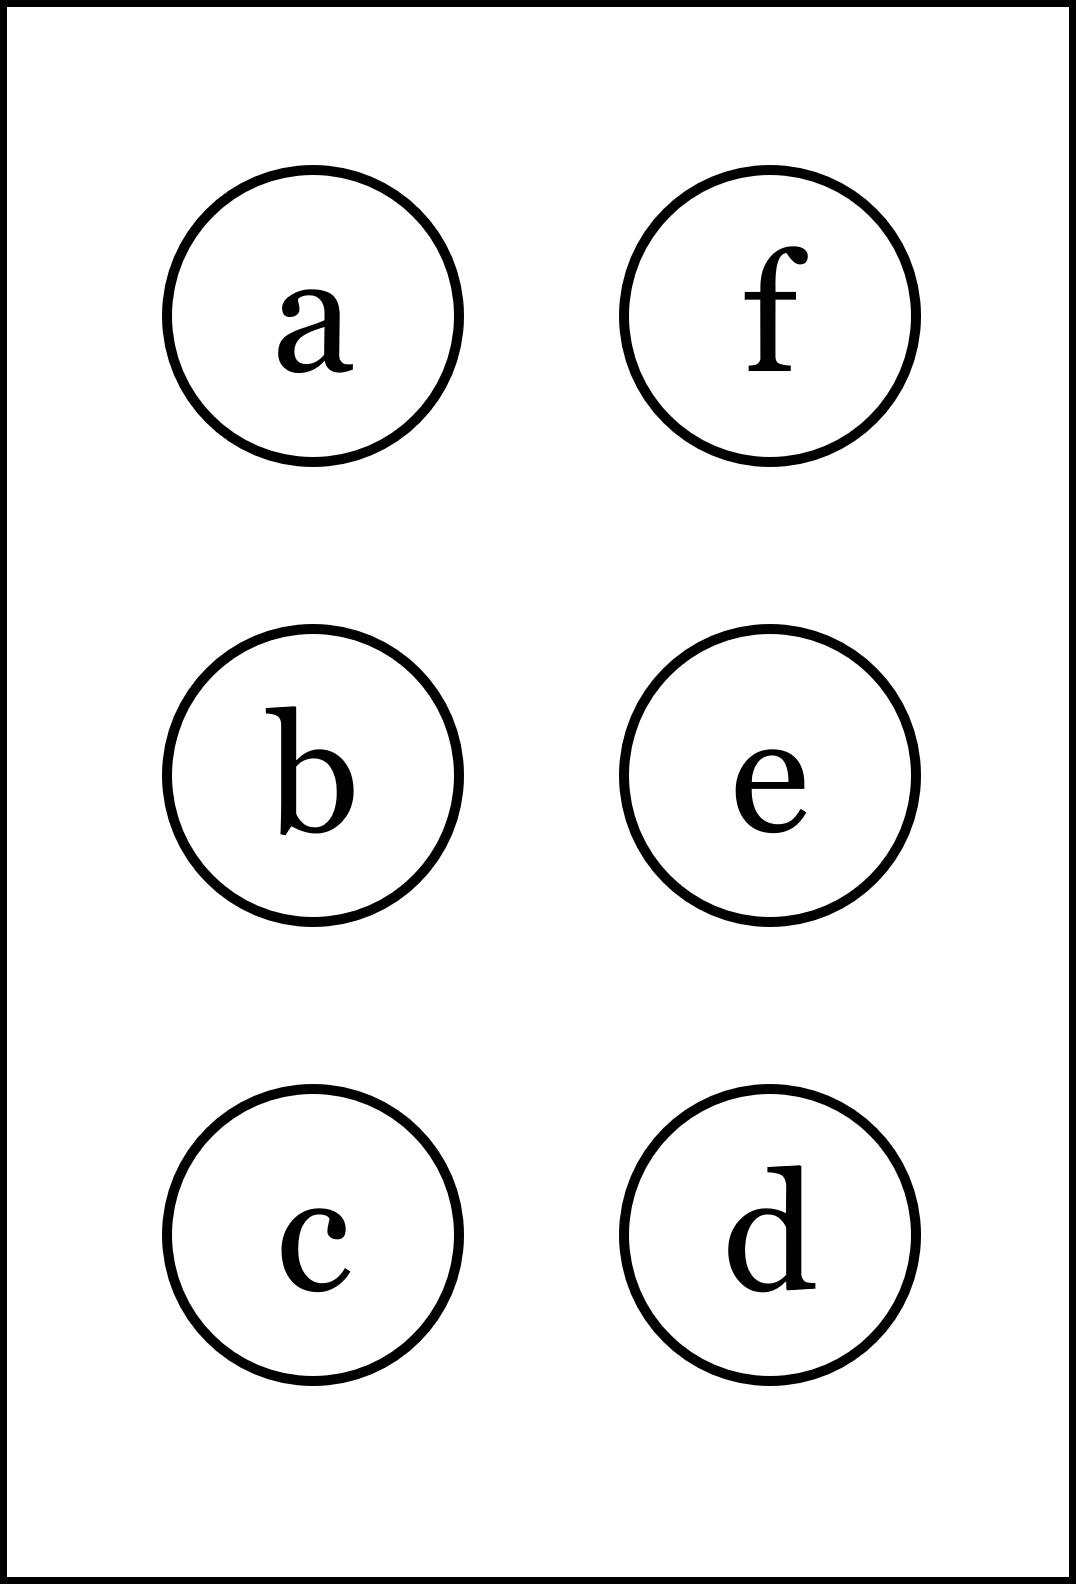
\includegraphics[height=40mm]{../images/braille.png}
{\small Písmeno Braillovej abecedy}
\end{center}
\end{minipage}
\end{center}
\end{minipage}
\\ \hdashline
\begin{minipage}[c][104.5mm][t]{0.5\linewidth}
\begin{center}
\vspace{7mm}
{\huge Stacionární body, skupina \textit{Zeta $\zeta$} -\romannumeral3}\\[5mm]
\textit{Jméno:}\phantom{xxxxxxxxxxxxxxxxxxxxxxxxxxxxxxxxxxxxxxxxxxxxxxxxxxxxxxxxxxxxxxxxx}\\[5mm]
\begin{minipage}{0.95\linewidth}
\begin{center}
{\small V \textbf{(a)} zjisti jestli $f(x)$ \textbf{roste} v bode $x_0$. V \textbf{(b)} zjisti jestli je $f(x)$ v bode $x_0$ \textbf{ryze konvexní}.\\V \textbf{(c)} spočti \textbf{součet} x-ových souřadnic stacionárního a inflexního bodu. V \textbf{(d)} najdi x-ovou souřadnici stacionárního bodu a rozhodli jestli to je \textbf{lomax, lomin či inflex}.\\Pokud se výsledky shodujú s těmi za otazníky, tak napravo obarvi příslušející kroužek načerno.\\\textbf{Spolu odevzdejte výsledné slovo}}.
\end{center}
\end{minipage}
\\[1mm]
\begin{minipage}{0.79\linewidth}
\begin{center}
\begin{varwidth}{\linewidth}
\begin{enumerate}
\normalsize
\item $f(x)=\cfrac{x^2+3x+3}{-x+9}\enspace , \enspace x_0=1$\quad \dotfill\; ???\;\dotfill \quad \text{ne}
\item $f(x)=x^4+2x^3-5x^2-x+2\enspace , \enspace x_0=-1$\quad \dotfill\; ???\;\dotfill \quad \text{ne}
\item $f(x)=-4xe^{3x}$\quad \dotfill\; ???\;\dotfill \quad $-1$
\item $f(x)=\sqrt{4x^2+4x+3}$\quad \dotfill\; ???\;\dotfill \quad $\nicefrac{-1}{2}\enspace , \enspace\mathrm{inflex}$
\item \quad \dotfill\; ???\;\dotfill \quad vybarvi
\item \quad \dotfill\; ???\;\dotfill \quad vybarvi
\end{enumerate}
\end{varwidth}
\end{center}
\end{minipage}
\begin{minipage}{0.20\linewidth}
\begin{center}
{\Huge\bfseries 3.} \\[2mm]
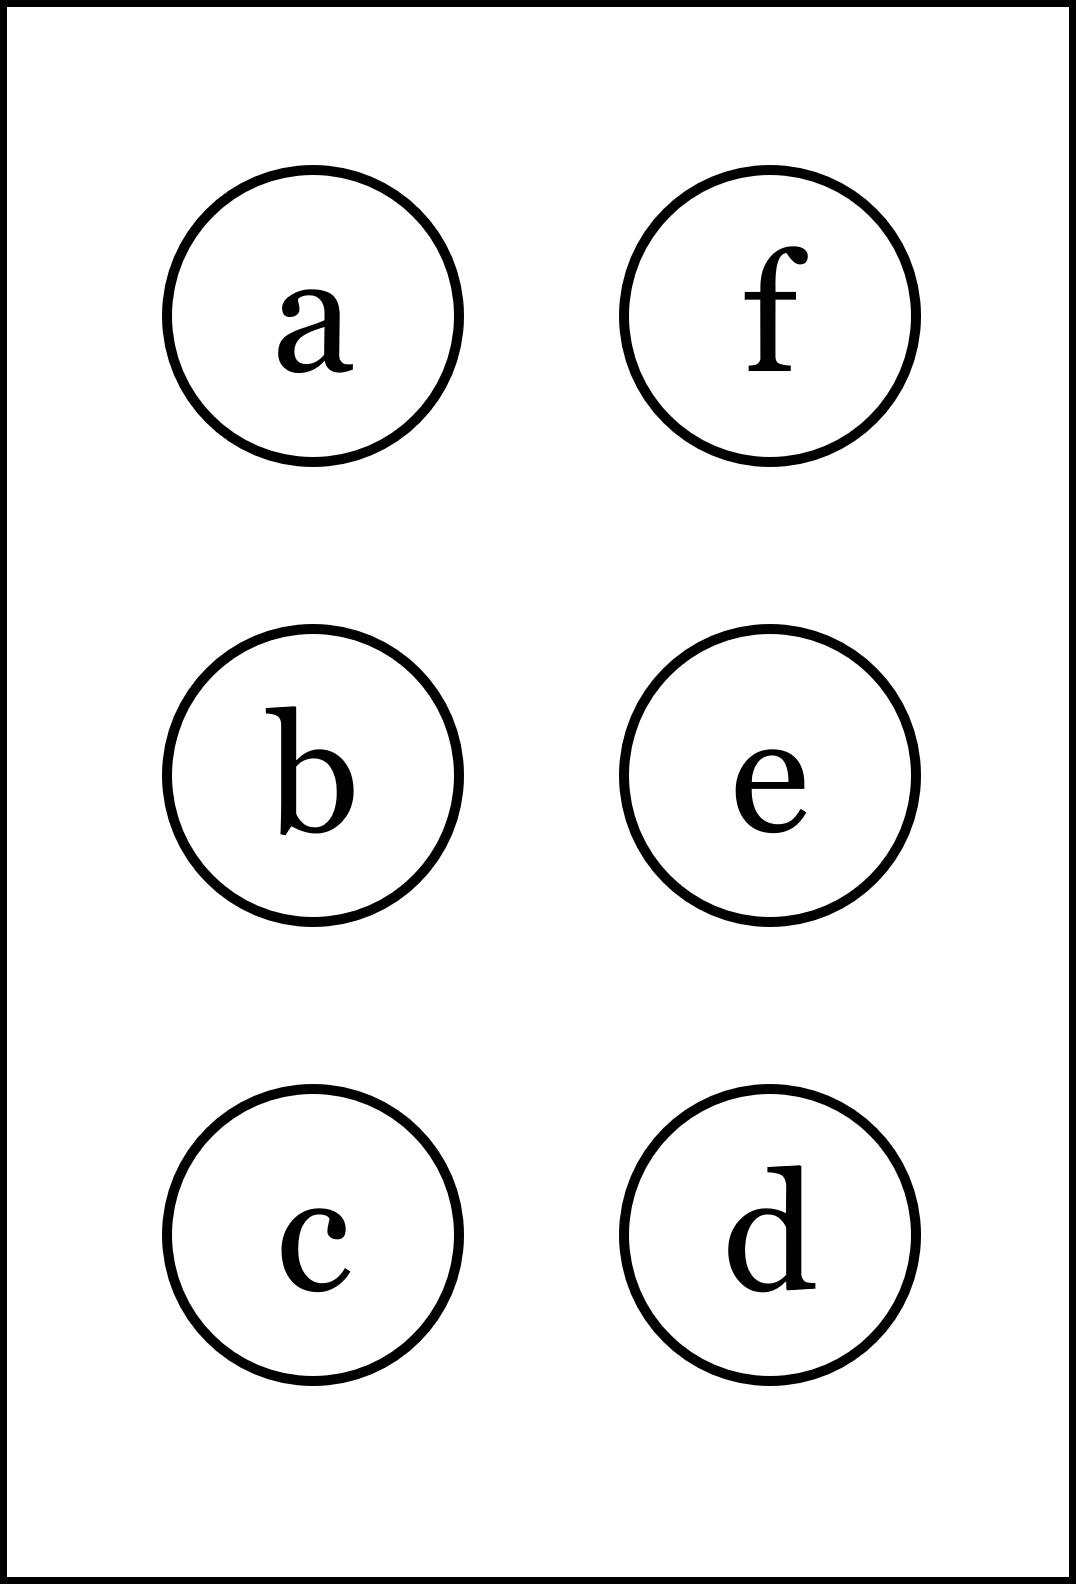
\includegraphics[height=40mm]{../images/braille.png}
{\small Písmeno Braillovej abecedy}
\end{center}
\end{minipage}
\end{center}
\end{minipage}
&
\begin{minipage}[c][104.5mm][t]{0.5\linewidth}
\begin{center}
\vspace{7mm}
{\huge Stacionární body, skupina \textit{Zeta $\zeta$} -\romannumeral4}\\[5mm]
\textit{Jméno:}\phantom{xxxxxxxxxxxxxxxxxxxxxxxxxxxxxxxxxxxxxxxxxxxxxxxxxxxxxxxxxxxxxxxxx}\\[5mm]
\begin{minipage}{0.95\linewidth}
\begin{center}
{\small V \textbf{(a)} zjisti jestli $f(x)$ \textbf{roste} v bode $x_0$. V \textbf{(b)} zjisti jestli je $f(x)$ v bode $x_0$ \textbf{ryze konvexní}.\\V \textbf{(c)} spočti \textbf{součet} x-ových souřadnic stacionárního a inflexního bodu. V \textbf{(d)} najdi x-ovou souřadnici stacionárního bodu a rozhodli jestli to je \textbf{lomax, lomin či inflex}.\\Pokud se výsledky shodujú s těmi za otazníky, tak napravo obarvi příslušející kroužek načerno.\\\textbf{Spolu odevzdejte výsledné slovo}}.
\end{center}
\end{minipage}
\\[1mm]
\begin{minipage}{0.79\linewidth}
\begin{center}
\begin{varwidth}{\linewidth}
\begin{enumerate}
\normalsize
\item $f(x)=\cfrac{-x^2+2x+3}{-2x-7}\enspace , \enspace x_0=7$\quad \dotfill\; ???\;\dotfill \quad \text{ano}
\item $f(x)=9x^4+x^3-6x^2+6x-4\enspace , \enspace x_0=-2$\quad \dotfill\; ???\;\dotfill \quad \text{ne}
\item $f(x)=xe^{-x}$\quad \dotfill\; ???\;\dotfill \quad $3$
\item $f(x)=\sqrt{2x^2+3x+4}$\quad \dotfill\; ???\;\dotfill \quad $\nicefrac{-3}{4}\enspace , \enspace\mathrm{lomax}$
\item \quad \dotfill\; ???\;\dotfill \quad vybarvi
\item \quad \dotfill\; ???\;\dotfill \quad nebarvi
\end{enumerate}
\end{varwidth}
\end{center}
\end{minipage}
\begin{minipage}{0.20\linewidth}
\begin{center}
{\Huge\bfseries 4.} \\[2mm]
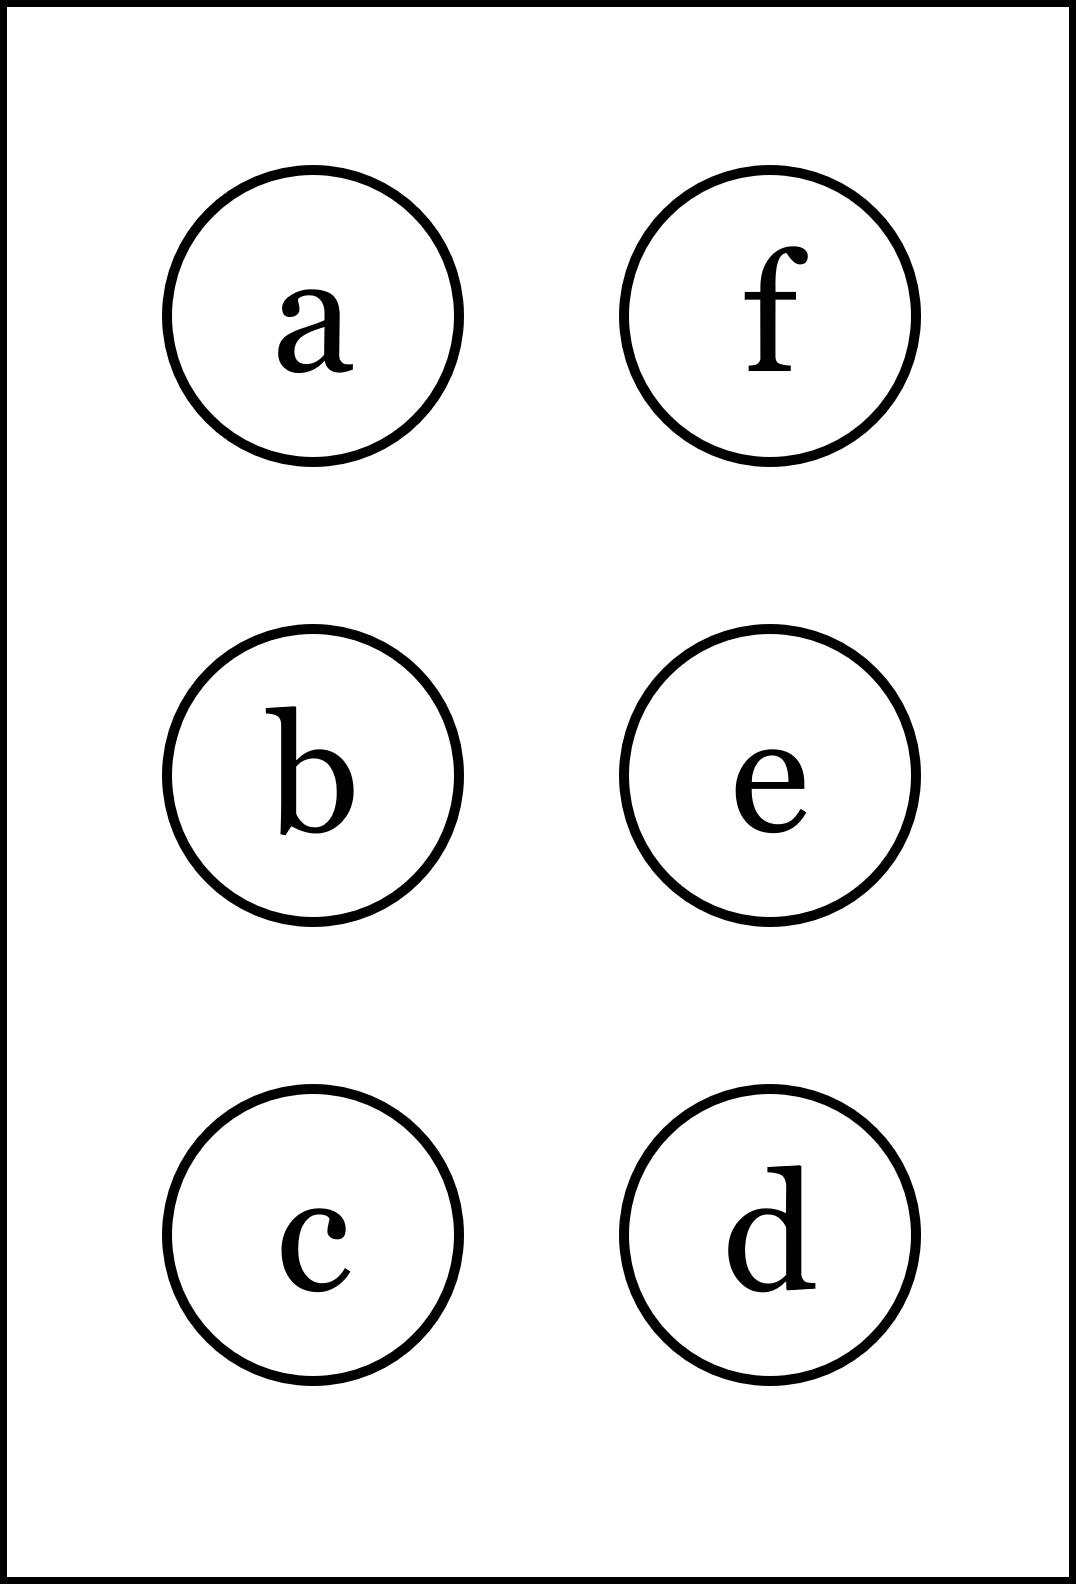
\includegraphics[height=40mm]{../images/braille.png}
{\small Písmeno Braillovej abecedy}
\end{center}
\end{minipage}
\end{center}
\end{minipage}
%
\end{tabular}
\newpage
\thispagestyle{empty}
\begin{tabular}{c:c}
\begin{minipage}[c][104.5mm][t]{0.5\linewidth}
\begin{center}
\vspace{7mm}
{\huge Stacionární body, skupina \textit{Eta $\eta$} -\romannumeral1}\\[5mm]
\textit{Jméno:}\phantom{xxxxxxxxxxxxxxxxxxxxxxxxxxxxxxxxxxxxxxxxxxxxxxxxxxxxxxxxxxxxxxxxx}\\[5mm]
\begin{minipage}{0.95\linewidth}
\begin{center}
{\small V \textbf{(a)} zjisti jestli $f(x)$ \textbf{roste} v bode $x_0$. V \textbf{(b)} zjisti jestli je $f(x)$ v bode $x_0$ \textbf{ryze konvexní}.\\V \textbf{(c)} spočti \textbf{součet} x-ových souřadnic stacionárního a inflexního bodu. V \textbf{(d)} najdi x-ovou souřadnici stacionárního bodu a rozhodli jestli to je \textbf{lomax, lomin či inflex}.\\Pokud se výsledky shodujú s těmi za otazníky, tak napravo obarvi příslušející kroužek načerno.\\\textbf{Spolu odevzdejte výsledné slovo}}.
\end{center}
\end{minipage}
\\[1mm]
\begin{minipage}{0.79\linewidth}
\begin{center}
\begin{varwidth}{\linewidth}
\begin{enumerate}
\normalsize
\item $f(x)=\cfrac{2x^2-5x-2}{-2x+1}\enspace , \enspace x_0=4$\quad \dotfill\; ???\;\dotfill \quad \text{ano}
\item $f(x)=-x^4+4x^3-8x^2+7x-6\enspace , \enspace x_0=3$\quad \dotfill\; ???\;\dotfill \quad \text{ano}
\item $f(x)=4xe^{-5x}$\quad \dotfill\; ???\;\dotfill \quad $\nicefrac{3}{5}$
\item $f(x)=\sqrt{3x^2-5x+5}$\quad \dotfill\; ???\;\dotfill \quad $\nicefrac{5}{6}\enspace , \enspace \mathrm{lomin}$
\item \quad \dotfill\; ???\;\dotfill \quad nebarvi
\item \quad \dotfill\; ???\;\dotfill \quad vybarvi
\end{enumerate}
\end{varwidth}
\end{center}
\end{minipage}
\begin{minipage}{0.20\linewidth}
\begin{center}
{\Huge\bfseries 1.} \\[2mm]
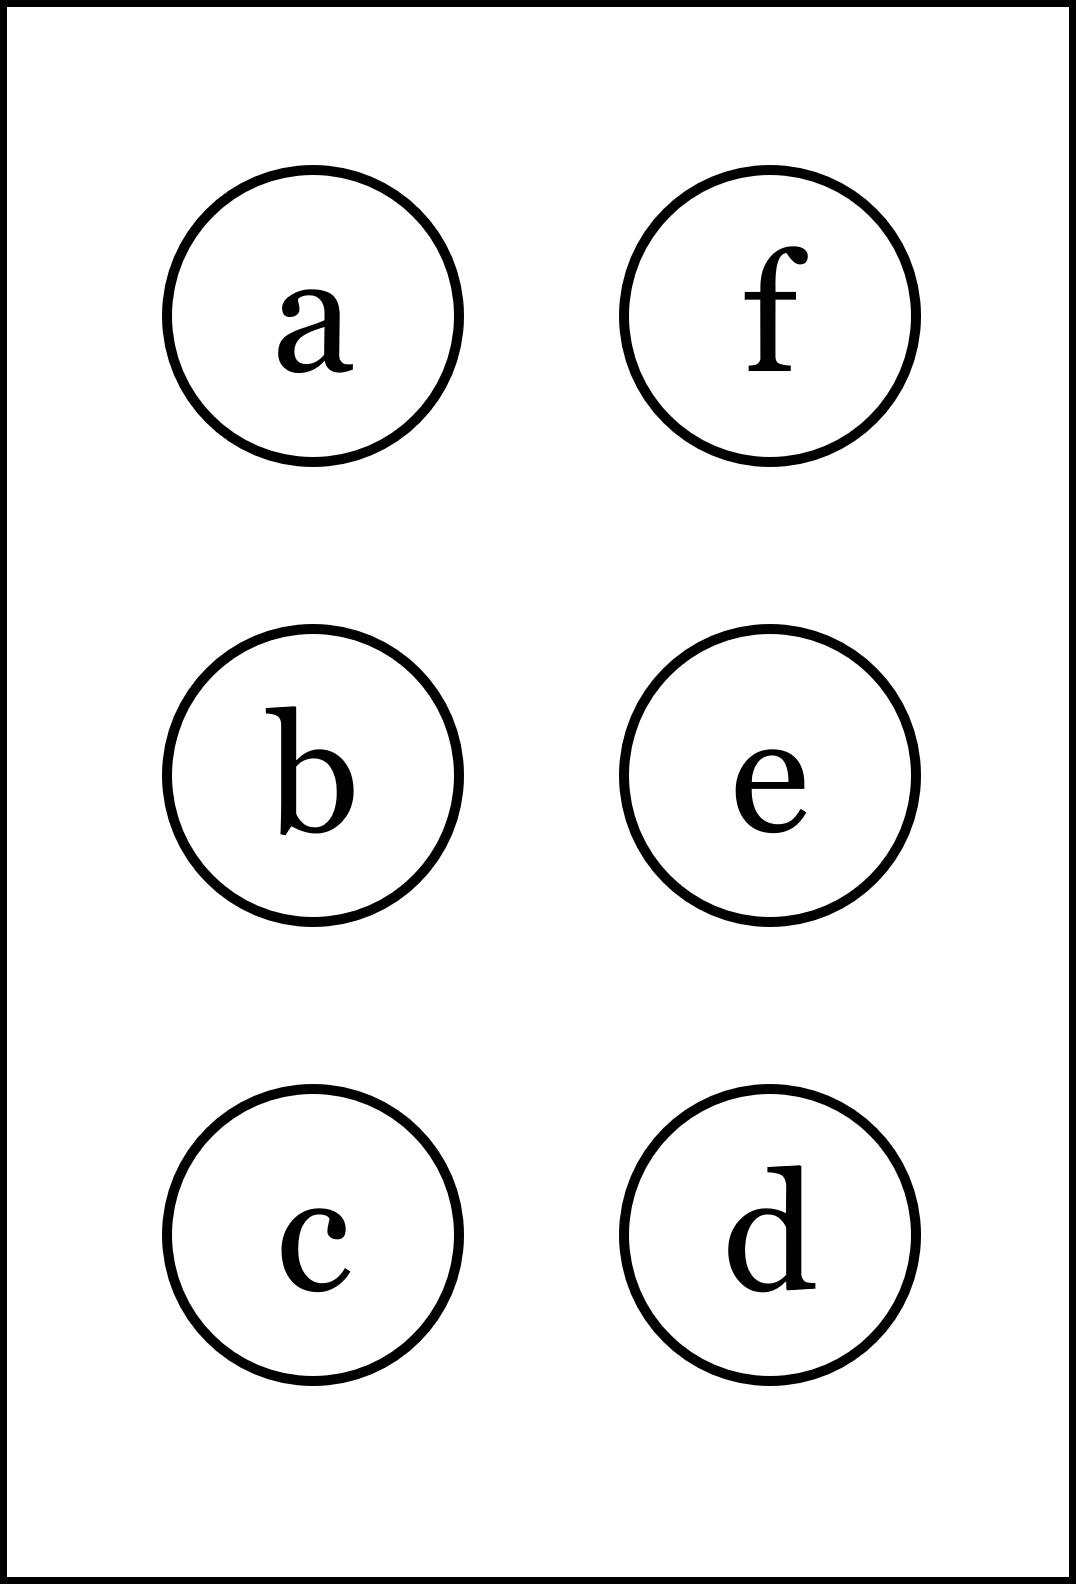
\includegraphics[height=40mm]{../images/braille.png}
{\small Písmeno Braillovej abecedy}
\end{center}
\end{minipage}
\end{center}
\end{minipage}
&
\begin{minipage}[c][104.5mm][t]{0.5\linewidth}
\begin{center}
\vspace{7mm}
{\huge Stacionární body, skupina \textit{Eta $\eta$} -\romannumeral2}\\[5mm]
\textit{Jméno:}\phantom{xxxxxxxxxxxxxxxxxxxxxxxxxxxxxxxxxxxxxxxxxxxxxxxxxxxxxxxxxxxxxxxxx}\\[5mm]
\begin{minipage}{0.95\linewidth}
\begin{center}
{\small V \textbf{(a)} zjisti jestli $f(x)$ \textbf{roste} v bode $x_0$. V \textbf{(b)} zjisti jestli je $f(x)$ v bode $x_0$ \textbf{ryze konvexní}.\\V \textbf{(c)} spočti \textbf{součet} x-ových souřadnic stacionárního a inflexního bodu. V \textbf{(d)} najdi x-ovou souřadnici stacionárního bodu a rozhodli jestli to je \textbf{lomax, lomin či inflex}.\\Pokud se výsledky shodujú s těmi za otazníky, tak napravo obarvi příslušející kroužek načerno.\\\textbf{Spolu odevzdejte výsledné slovo}}.
\end{center}
\end{minipage}
\\[1mm]
\begin{minipage}{0.79\linewidth}
\begin{center}
\begin{varwidth}{\linewidth}
\begin{enumerate}
\normalsize
\item $f(x)=\cfrac{2x^2+5x-5}{-x-3}\enspace , \enspace x_0=-4$\quad \dotfill\; ???\;\dotfill \quad \text{ne}
\item $f(x)=-x^4-8x^3+5x^2+x-3\enspace , \enspace x_0=-2$\quad \dotfill\; ???\;\dotfill \quad \text{ne}
\item $f(x)=xe^{-7x}$\quad \dotfill\; ???\;\dotfill \quad $\nicefrac{3}{7}$
\item $f(x)=\sqrt{3x^2+2x+3}$\quad \dotfill\; ???\;\dotfill \quad $\nicefrac{-1}{3}\enspace , \enspace\mathrm{lomax}$
\item \quad \dotfill\; ???\;\dotfill \quad nebarvi
\item \quad \dotfill\; ???\;\dotfill \quad nebarvi
\end{enumerate}
\end{varwidth}
\end{center}
\end{minipage}
\begin{minipage}{0.20\linewidth}
\begin{center}
{\Huge\bfseries 2.} \\[2mm]
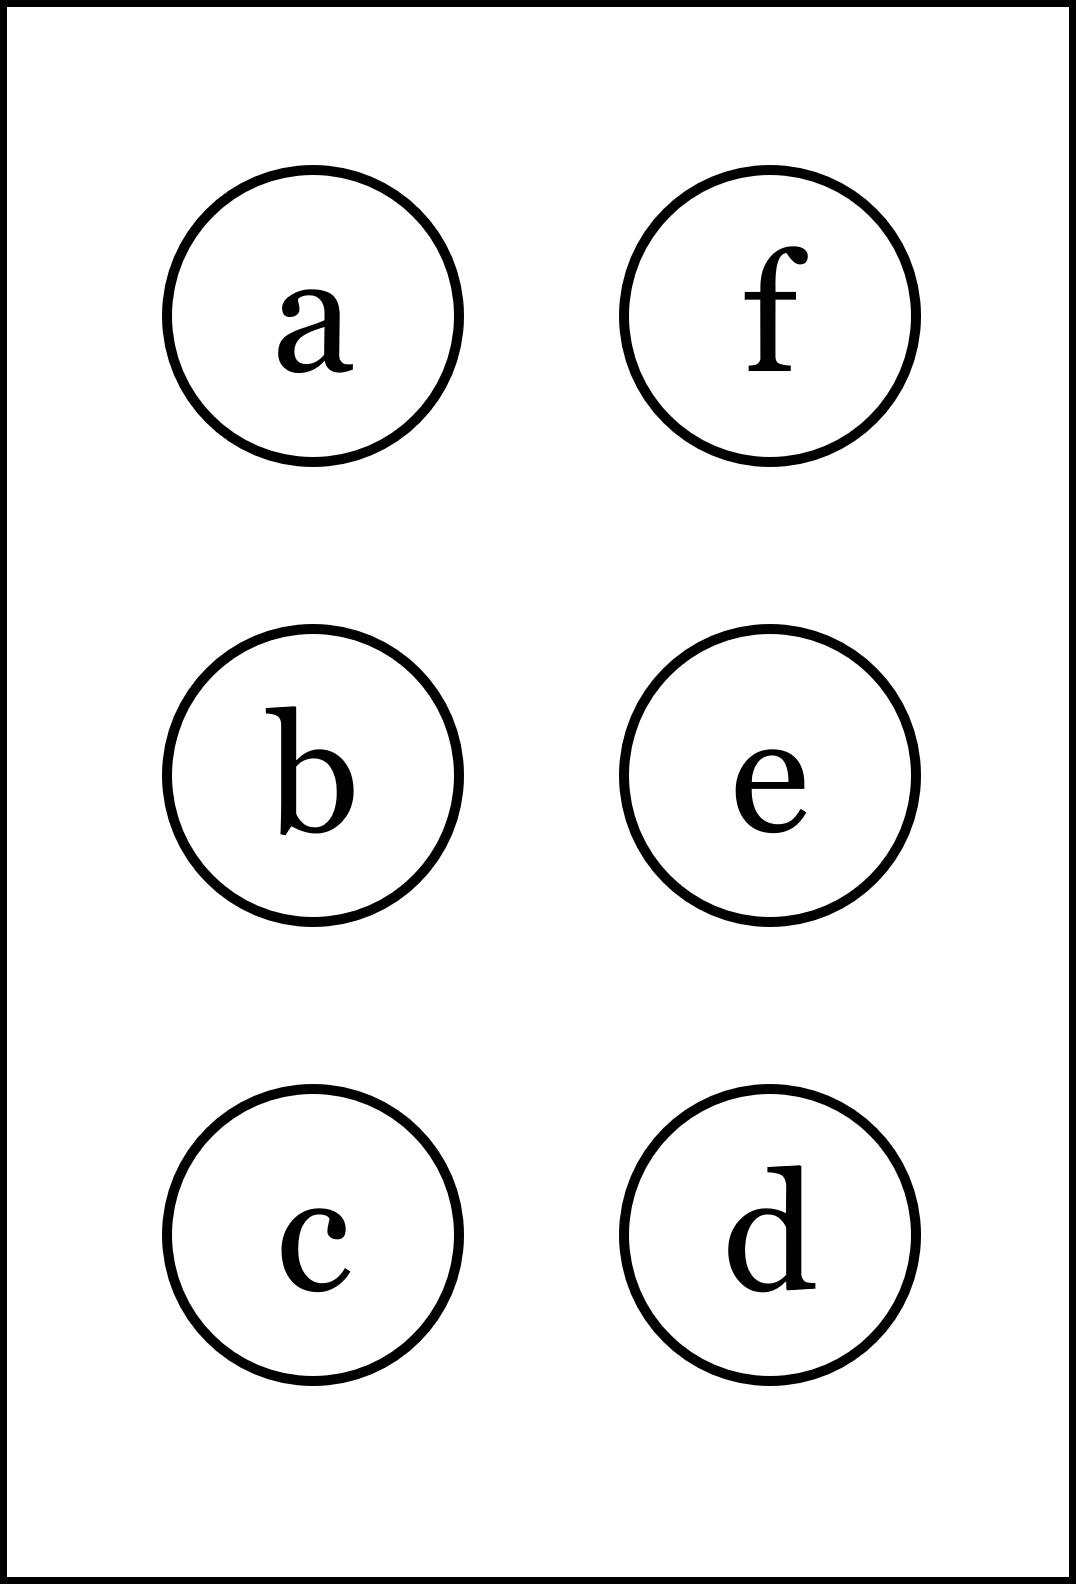
\includegraphics[height=40mm]{../images/braille.png}
{\small Písmeno Braillovej abecedy}
\end{center}
\end{minipage}
\end{center}
\end{minipage}
\\ \hdashline
\begin{minipage}[c][104.5mm][t]{0.5\linewidth}
\begin{center}
\vspace{7mm}
{\huge Stacionární body, skupina \textit{Eta $\eta$} -\romannumeral3}\\[5mm]
\textit{Jméno:}\phantom{xxxxxxxxxxxxxxxxxxxxxxxxxxxxxxxxxxxxxxxxxxxxxxxxxxxxxxxxxxxxxxxxx}\\[5mm]
\begin{minipage}{0.95\linewidth}
\begin{center}
{\small V \textbf{(a)} zjisti jestli $f(x)$ \textbf{roste} v bode $x_0$. V \textbf{(b)} zjisti jestli je $f(x)$ v bode $x_0$ \textbf{ryze konvexní}.\\V \textbf{(c)} spočti \textbf{součet} x-ových souřadnic stacionárního a inflexního bodu. V \textbf{(d)} najdi x-ovou souřadnici stacionárního bodu a rozhodli jestli to je \textbf{lomax, lomin či inflex}.\\Pokud se výsledky shodujú s těmi za otazníky, tak napravo obarvi příslušející kroužek načerno.\\\textbf{Spolu odevzdejte výsledné slovo}}.
\end{center}
\end{minipage}
\\[1mm]
\begin{minipage}{0.79\linewidth}
\begin{center}
\begin{varwidth}{\linewidth}
\begin{enumerate}
\normalsize
\item $f(x)=\cfrac{-x^2-x+4}{2x-7}\enspace , \enspace x_0=6$\quad \dotfill\; ???\;\dotfill \quad \text{ano}
\item $f(x)=2x^4+x^3+2x^2+x-4\enspace , \enspace x_0=2$\quad \dotfill\; ???\;\dotfill \quad \text{ne}
\item $f(x)=5xe^{x}$\quad \dotfill\; ???\;\dotfill \quad $-3$
\item $f(x)=\sqrt{3x^2+5x+4}$\quad \dotfill\; ???\;\dotfill \quad $\nicefrac{-5}{6}\enspace , \enspace\mathrm{lomax}$
\item \quad \dotfill\; ???\;\dotfill \quad vybarvi
\item \quad \dotfill\; ???\;\dotfill \quad nebarvi
\end{enumerate}
\end{varwidth}
\end{center}
\end{minipage}
\begin{minipage}{0.20\linewidth}
\begin{center}
{\Huge\bfseries 3.} \\[2mm]
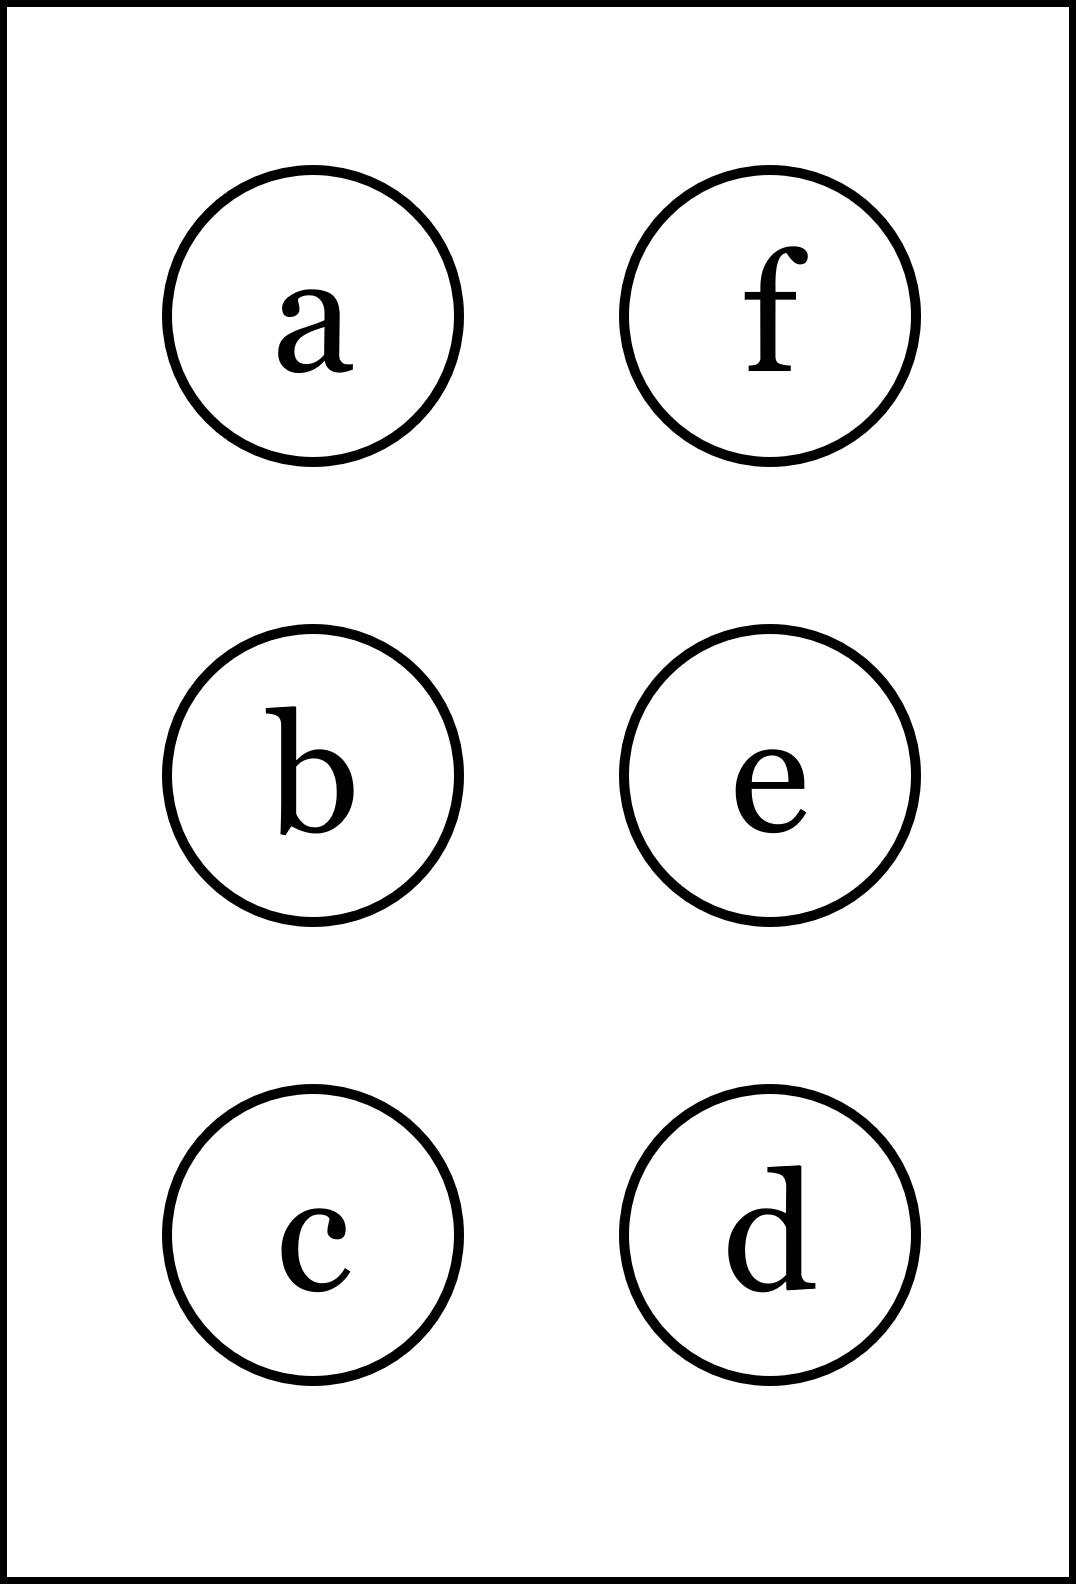
\includegraphics[height=40mm]{../images/braille.png}
{\small Písmeno Braillovej abecedy}
\end{center}
\end{minipage}
\end{center}
\end{minipage}
&
\begin{minipage}[c][104.5mm][t]{0.5\linewidth}
\begin{center}
\vspace{7mm}
{\huge Stacionární body, skupina \textit{Eta $\eta$} -\romannumeral4}\\[5mm]
\textit{Jméno:}\phantom{xxxxxxxxxxxxxxxxxxxxxxxxxxxxxxxxxxxxxxxxxxxxxxxxxxxxxxxxxxxxxxxxx}\\[5mm]
\begin{minipage}{0.95\linewidth}
\begin{center}
{\small V \textbf{(a)} zjisti jestli $f(x)$ \textbf{roste} v bode $x_0$. V \textbf{(b)} zjisti jestli je $f(x)$ v bode $x_0$ \textbf{ryze konvexní}.\\V \textbf{(c)} spočti \textbf{součet} x-ových souřadnic stacionárního a inflexního bodu. V \textbf{(d)} najdi x-ovou souřadnici stacionárního bodu a rozhodli jestli to je \textbf{lomax, lomin či inflex}.\\Pokud se výsledky shodujú s těmi za otazníky, tak napravo obarvi příslušející kroužek načerno.\\\textbf{Spolu odevzdejte výsledné slovo}}.
\end{center}
\end{minipage}
\\[1mm]
\begin{minipage}{0.79\linewidth}
\begin{center}
\begin{varwidth}{\linewidth}
\begin{enumerate}
\normalsize
\item $f(x)=\cfrac{-x^2-5x-5}{x+1}\enspace , \enspace x_0=6$\quad \dotfill\; ???\;\dotfill \quad \text{ne}
\item $f(x)=2x^4-x^3-x^2-6x+1\enspace , \enspace x_0=2$\quad \dotfill\; ???\;\dotfill \quad \text{ano}
\item $f(x)=xe^{2x}$\quad \dotfill\; ???\;\dotfill \quad $\nicefrac{-3}{2}$
\item $f(x)=\sqrt{5x^2+x+2}$\quad \dotfill\; ???\;\dotfill \quad $\nicefrac{-1}{10}\enspace , \enspace\mathrm{lomax}$
\item \quad \dotfill\; ???\;\dotfill \quad nebarvi
\item \quad \dotfill\; ???\;\dotfill \quad nebarvi
\end{enumerate}
\end{varwidth}
\end{center}
\end{minipage}
\begin{minipage}{0.20\linewidth}
\begin{center}
{\Huge\bfseries 4.} \\[2mm]
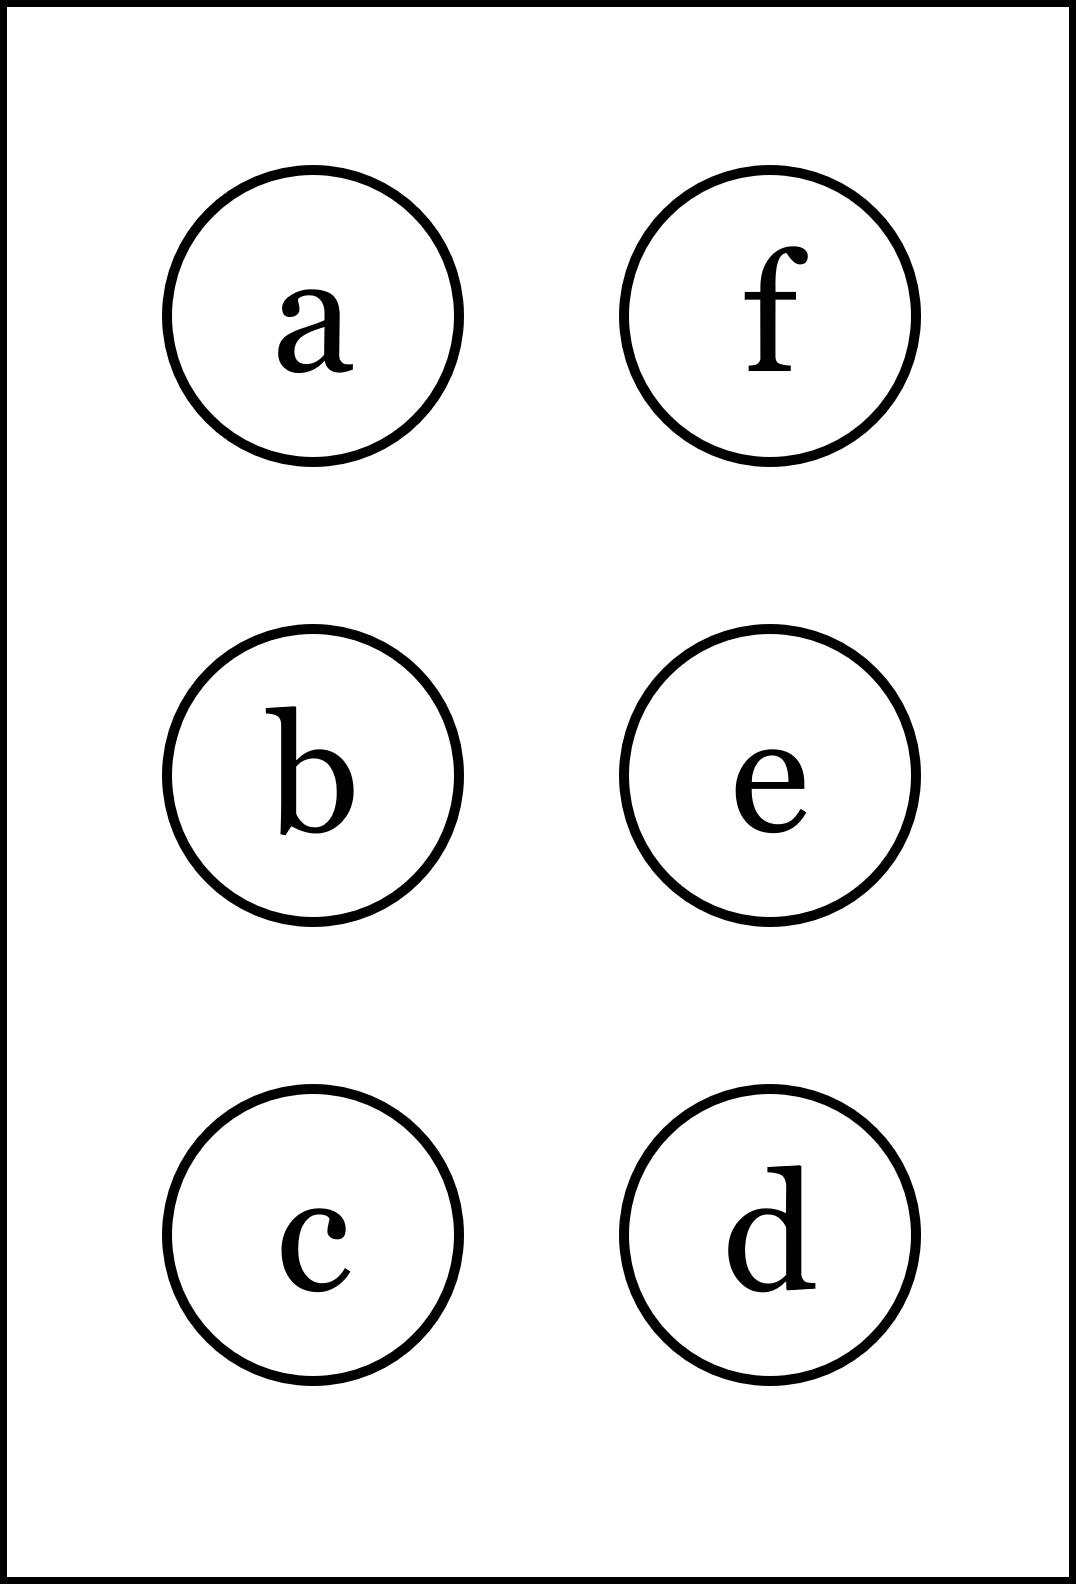
\includegraphics[height=40mm]{../images/braille.png}
{\small Písmeno Braillovej abecedy}
\end{center}
\end{minipage}
\end{center}
\end{minipage}
%
\end{tabular}
\newpage
\thispagestyle{empty}
\begin{tabular}{c:c}
\begin{minipage}[c][104.5mm][t]{0.5\linewidth}
\begin{center}
\vspace{7mm}
{\huge Stacionární body, skupina \textit{Theta $\theta$} -\romannumeral1}\\[5mm]
\textit{Jméno:}\phantom{xxxxxxxxxxxxxxxxxxxxxxxxxxxxxxxxxxxxxxxxxxxxxxxxxxxxxxxxxxxxxxxxx}\\[5mm]
\begin{minipage}{0.95\linewidth}
\begin{center}
{\small V \textbf{(a)} zjisti jestli $f(x)$ \textbf{roste} v bode $x_0$. V \textbf{(b)} zjisti jestli je $f(x)$ v bode $x_0$ \textbf{ryze konvexní}.\\V \textbf{(c)} spočti \textbf{součet} x-ových souřadnic stacionárního a inflexního bodu. V \textbf{(d)} najdi x-ovou souřadnici stacionárního bodu a rozhodli jestli to je \textbf{lomax, lomin či inflex}.\\Pokud se výsledky shodujú s těmi za otazníky, tak napravo obarvi příslušející kroužek načerno.\\\textbf{Spolu odevzdejte výsledné slovo}}.
\end{center}
\end{minipage}
\\[1mm]
\begin{minipage}{0.79\linewidth}
\begin{center}
\begin{varwidth}{\linewidth}
\begin{enumerate}
\normalsize
\item $f(x)=\cfrac{-x^2+5x-9}{-x-2}\enspace , \enspace x_0=1$\quad \dotfill\; ???\;\dotfill \quad \text{ne}
\item $f(x)=x^4+2x^3-3x^2-8x-5\enspace , \enspace x_0=4$\quad \dotfill\; ???\;\dotfill \quad \text{ne}
\item $f(x)=3xe^{-x}$\quad \dotfill\; ???\;\dotfill \quad $3$
\item $f(x)=\sqrt{x^2-3x+4}$\quad \dotfill\; ???\;\dotfill \quad $\nicefrac{3}{2}\enspace , \enspace\mathrm{inflex}$
\item \quad \dotfill\; ???\;\dotfill \quad nebarvi
\item \quad \dotfill\; ???\;\dotfill \quad vybarvi
\end{enumerate}
\end{varwidth}
\end{center}
\end{minipage}
\begin{minipage}{0.20\linewidth}
\begin{center}
{\Huge\bfseries 1.} \\[2mm]
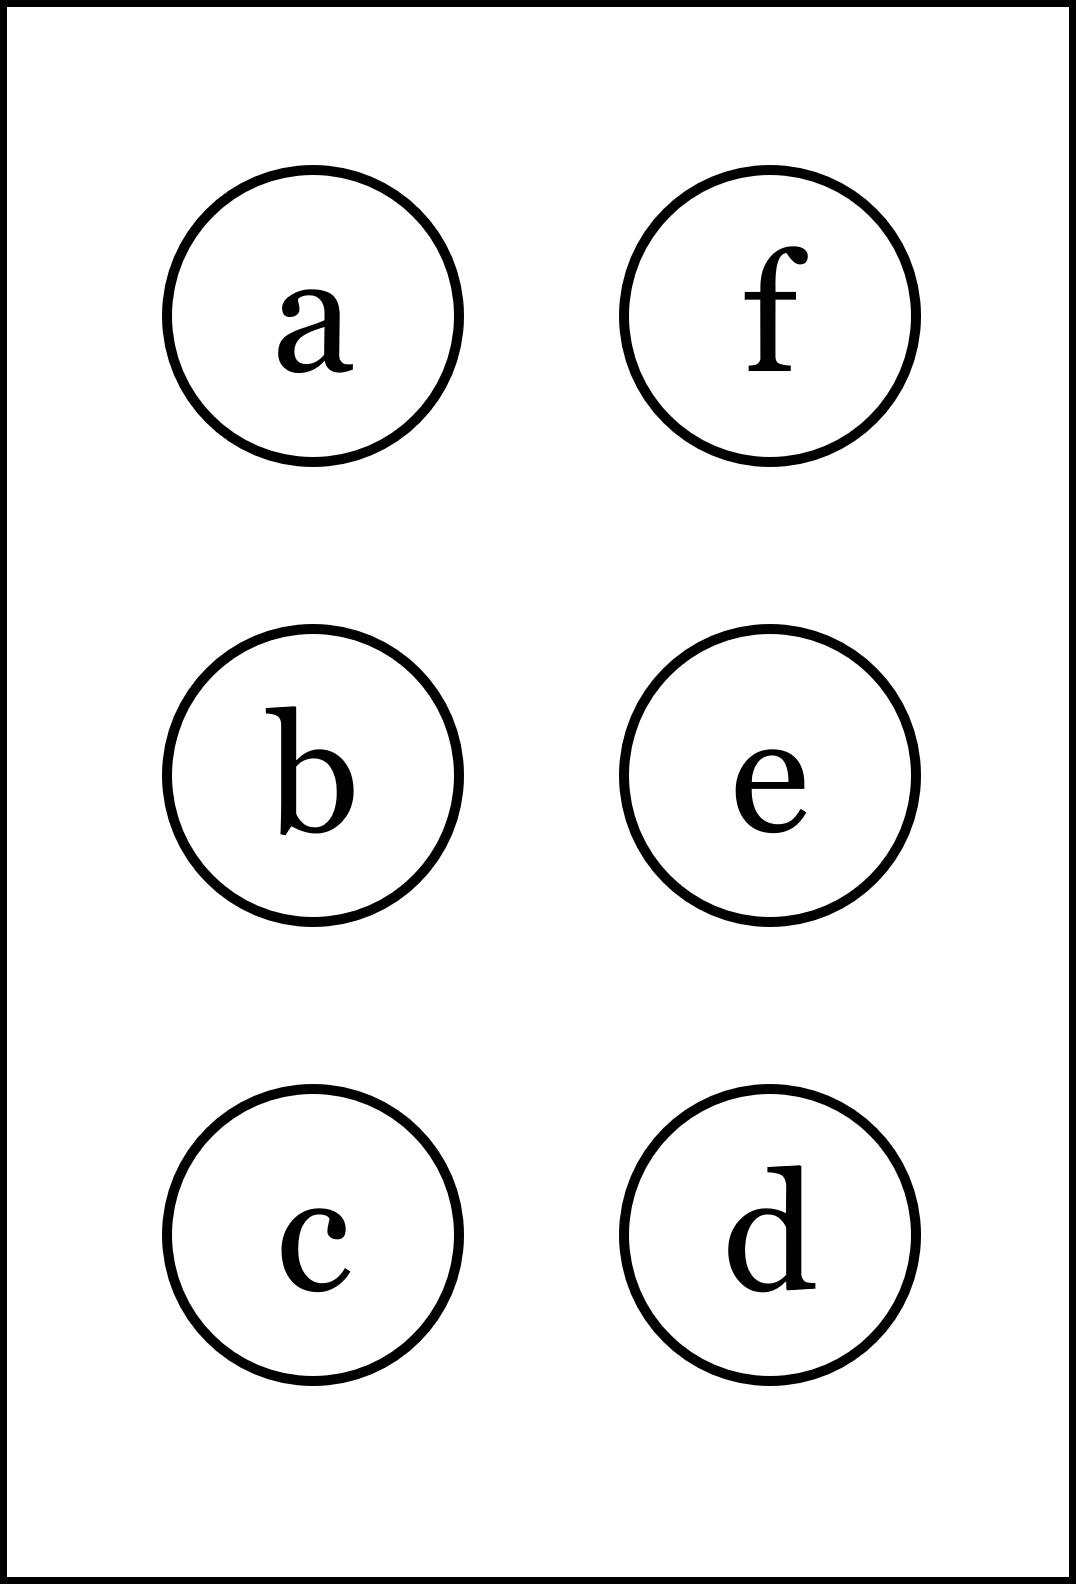
\includegraphics[height=40mm]{../images/braille.png}
{\small Písmeno Braillovej abecedy}
\end{center}
\end{minipage}
\end{center}
\end{minipage}
&
\begin{minipage}[c][104.5mm][t]{0.5\linewidth}
\begin{center}
\vspace{7mm}
{\huge Stacionární body, skupina \textit{Theta $\theta$} -\romannumeral2}\\[5mm]
\textit{Jméno:}\phantom{xxxxxxxxxxxxxxxxxxxxxxxxxxxxxxxxxxxxxxxxxxxxxxxxxxxxxxxxxxxxxxxxx}\\[5mm]
\begin{minipage}{0.95\linewidth}
\begin{center}
{\small V \textbf{(a)} zjisti jestli $f(x)$ \textbf{roste} v bode $x_0$. V \textbf{(b)} zjisti jestli je $f(x)$ v bode $x_0$ \textbf{ryze konvexní}.\\V \textbf{(c)} spočti \textbf{součet} x-ových souřadnic stacionárního a inflexního bodu. V \textbf{(d)} najdi x-ovou souřadnici stacionárního bodu a rozhodli jestli to je \textbf{lomax, lomin či inflex}.\\Pokud se výsledky shodujú s těmi za otazníky, tak napravo obarvi příslušející kroužek načerno.\\\textbf{Spolu odevzdejte výsledné slovo}}.
\end{center}
\end{minipage}
\\[1mm]
\begin{minipage}{0.79\linewidth}
\begin{center}
\begin{varwidth}{\linewidth}
\begin{enumerate}
\normalsize
\item $f(x)=\cfrac{2x^2-3x-8}{-2x+1}\enspace , \enspace x_0=-2$\quad \dotfill\; ???\;\dotfill \quad \text{ne}
\item $f(x)=-9x^4-4x^3-5x^2+7x+2\enspace , \enspace x_0=-1$\quad \dotfill\; ???\;\dotfill \quad \text{ano}
\item $f(x)=-xe^{-4x}$\quad \dotfill\; ???\;\dotfill \quad $\nicefrac{-1}{4}$
\item $f(x)=\sqrt{2x^2-x+1}$\quad \dotfill\; ???\;\dotfill \quad $\nicefrac{1}{4}\enspace , \enspace \mathrm{lomin}$
\item \quad \dotfill\; ???\;\dotfill \quad nebarvi
\item \quad \dotfill\; ???\;\dotfill \quad nebarvi
\end{enumerate}
\end{varwidth}
\end{center}
\end{minipage}
\begin{minipage}{0.20\linewidth}
\begin{center}
{\Huge\bfseries 2.} \\[2mm]
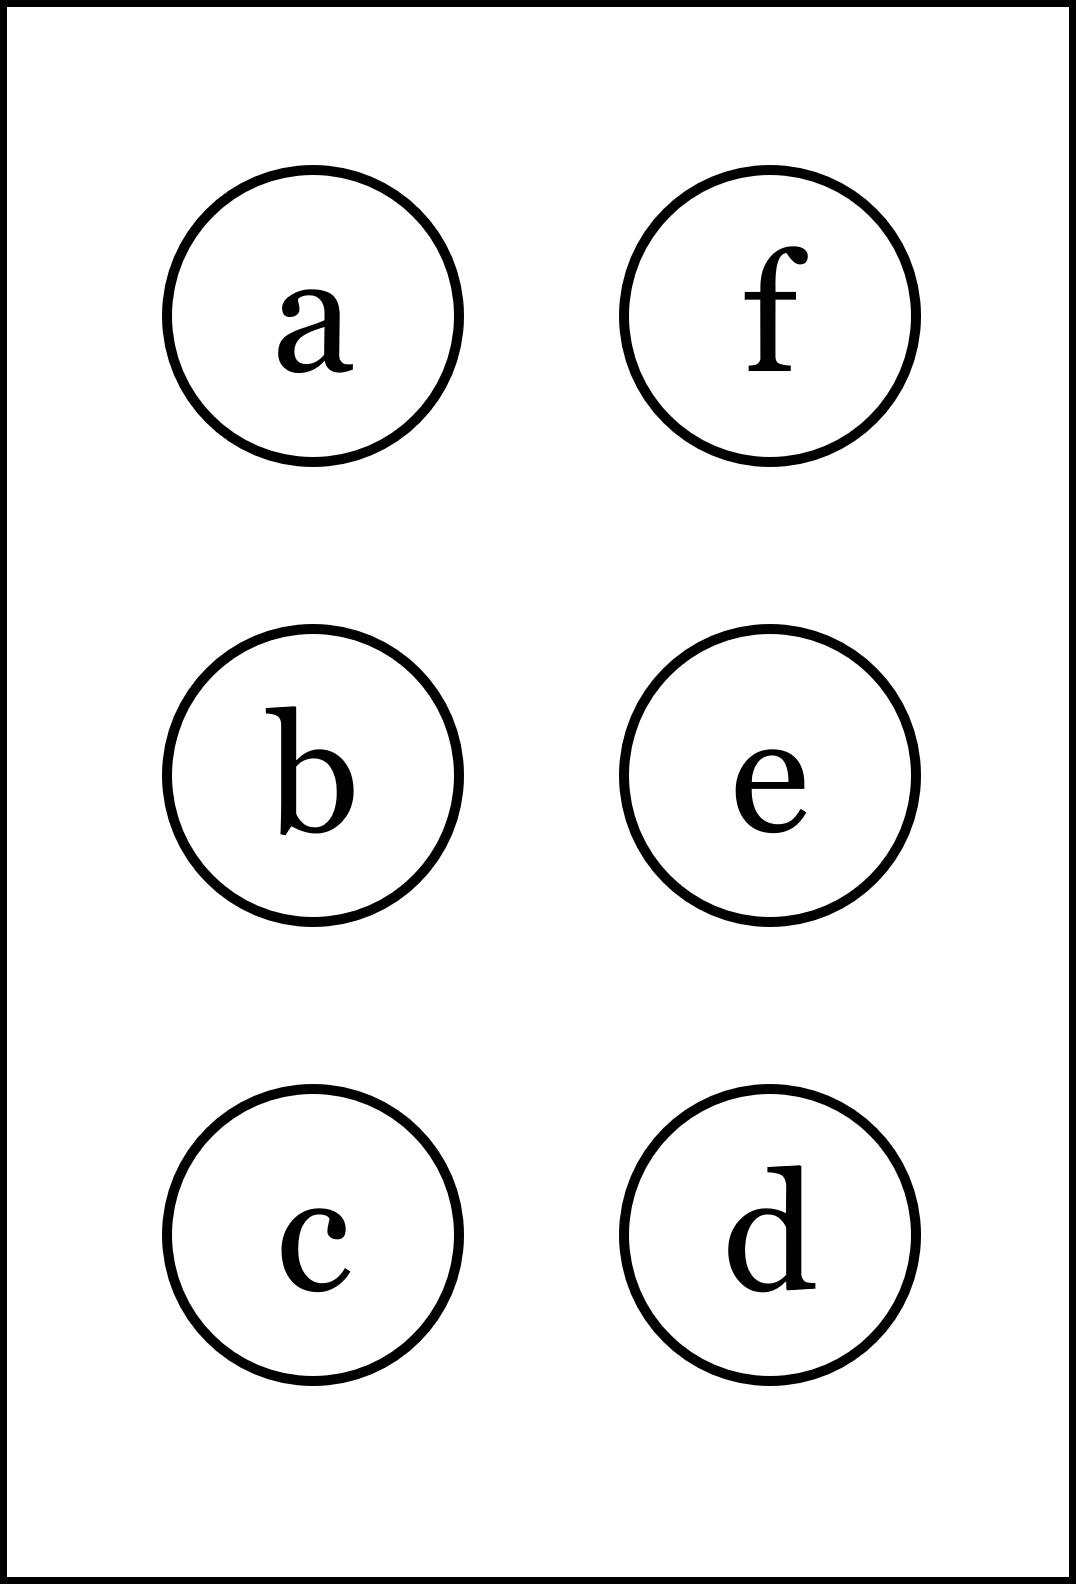
\includegraphics[height=40mm]{../images/braille.png}
{\small Písmeno Braillovej abecedy}
\end{center}
\end{minipage}
\end{center}
\end{minipage}
\\ \hdashline
\begin{minipage}[c][104.5mm][t]{0.5\linewidth}
\begin{center}
\vspace{7mm}
{\huge Stacionární body, skupina \textit{Theta $\theta$} -\romannumeral3}\\[5mm]
\textit{Jméno:}\phantom{xxxxxxxxxxxxxxxxxxxxxxxxxxxxxxxxxxxxxxxxxxxxxxxxxxxxxxxxxxxxxxxxx}\\[5mm]
\begin{minipage}{0.95\linewidth}
\begin{center}
{\small V \textbf{(a)} zjisti jestli $f(x)$ \textbf{roste} v bode $x_0$. V \textbf{(b)} zjisti jestli je $f(x)$ v bode $x_0$ \textbf{ryze konvexní}.\\V \textbf{(c)} spočti \textbf{součet} x-ových souřadnic stacionárního a inflexního bodu. V \textbf{(d)} najdi x-ovou souřadnici stacionárního bodu a rozhodli jestli to je \textbf{lomax, lomin či inflex}.\\Pokud se výsledky shodujú s těmi za otazníky, tak napravo obarvi příslušející kroužek načerno.\\\textbf{Spolu odevzdejte výsledné slovo}}.
\end{center}
\end{minipage}
\\[1mm]
\begin{minipage}{0.79\linewidth}
\begin{center}
\begin{varwidth}{\linewidth}
\begin{enumerate}
\normalsize
\item $f(x)=\cfrac{x^2+5x+8}{-2x+1}\enspace , \enspace x_0=1$\quad \dotfill\; ???\;\dotfill \quad \text{ano}
\item $f(x)=x^4+3x^3-4x^2-6x-5\enspace , \enspace x_0=-1$\quad \dotfill\; ???\;\dotfill \quad \text{ano}
\item $f(x)=-4xe^{3x}$\quad \dotfill\; ???\;\dotfill \quad $-1$
\item $f(x)=\sqrt{2x^2-2x+3}$\quad \dotfill\; ???\;\dotfill \quad $\nicefrac{1}{2}\enspace , \enspace\mathrm{lomax}$
\item \quad \dotfill\; ???\;\dotfill \quad nebarvi
\item \quad \dotfill\; ???\;\dotfill \quad vybarvi
\end{enumerate}
\end{varwidth}
\end{center}
\end{minipage}
\begin{minipage}{0.20\linewidth}
\begin{center}
{\Huge\bfseries 3.} \\[2mm]
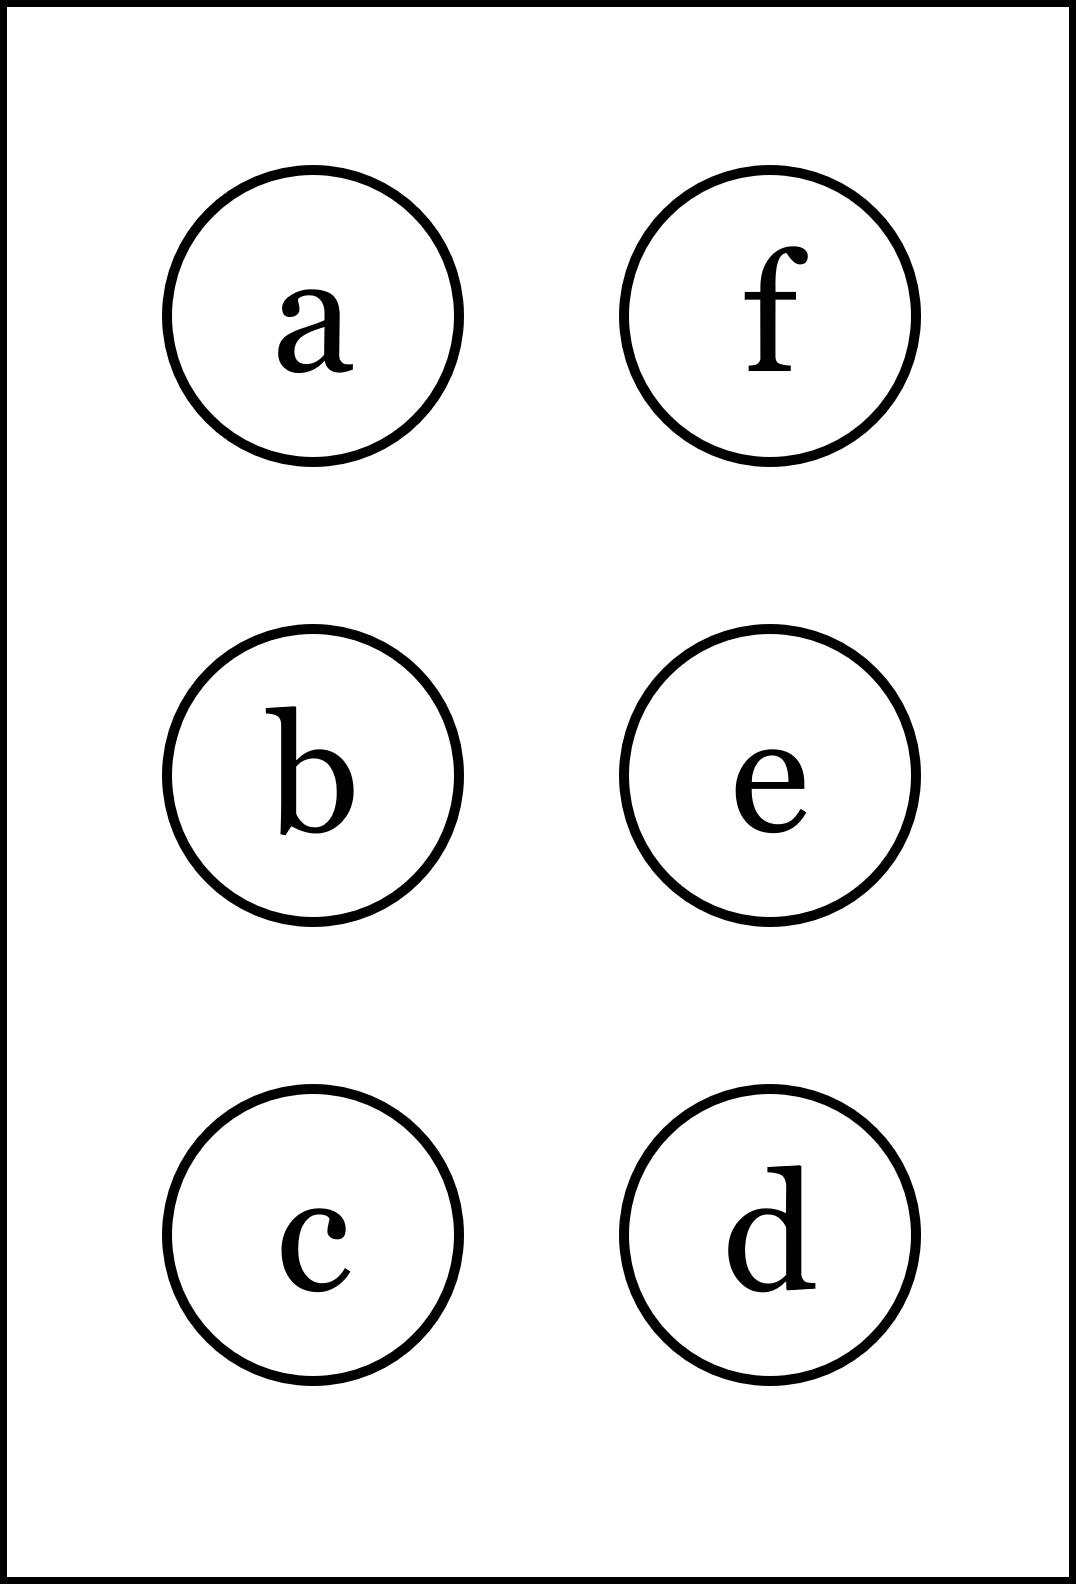
\includegraphics[height=40mm]{../images/braille.png}
{\small Písmeno Braillovej abecedy}
\end{center}
\end{minipage}
\end{center}
\end{minipage}
&
\begin{minipage}[c][104.5mm][t]{0.5\linewidth}
\begin{center}
\vspace{7mm}
{\huge Stacionární body, skupina \textit{Theta $\theta$} -\romannumeral4}\\[5mm]
\textit{Jméno:}\phantom{xxxxxxxxxxxxxxxxxxxxxxxxxxxxxxxxxxxxxxxxxxxxxxxxxxxxxxxxxxxxxxxxx}\\[5mm]
\begin{minipage}{0.95\linewidth}
\begin{center}
{\small V \textbf{(a)} zjisti jestli $f(x)$ \textbf{roste} v bode $x_0$. V \textbf{(b)} zjisti jestli je $f(x)$ v bode $x_0$ \textbf{ryze konvexní}.\\V \textbf{(c)} spočti \textbf{součet} x-ových souřadnic stacionárního a inflexního bodu. V \textbf{(d)} najdi x-ovou souřadnici stacionárního bodu a rozhodli jestli to je \textbf{lomax, lomin či inflex}.\\Pokud se výsledky shodujú s těmi za otazníky, tak napravo obarvi příslušející kroužek načerno.\\\textbf{Spolu odevzdejte výsledné slovo}}.
\end{center}
\end{minipage}
\\[1mm]
\begin{minipage}{0.79\linewidth}
\begin{center}
\begin{varwidth}{\linewidth}
\begin{enumerate}
\normalsize
\item $f(x)=\cfrac{-8x^2-5x-6}{-4x+3}\enspace , \enspace x_0=1$\quad \dotfill\; ???\;\dotfill \quad \text{ne}
\item $f(x)=2x^4+2x^3+2x^2-3x-4\enspace , \enspace x_0=1$\quad \dotfill\; ???\;\dotfill \quad \text{ne}
\item $f(x)=-xe^{2x}$\quad \dotfill\; ???\;\dotfill \quad $\nicefrac{1}{2}$
\item $f(x)=\sqrt{2x^2+3x+3}$\quad \dotfill\; ???\;\dotfill \quad $\nicefrac{-3}{4}\enspace , \enspace\mathrm{lomax}$
\item \quad \dotfill\; ???\;\dotfill \quad nebarvi
\item \quad \dotfill\; ???\;\dotfill \quad nebarvi
\end{enumerate}
\end{varwidth}
\end{center}
\end{minipage}
\begin{minipage}{0.20\linewidth}
\begin{center}
{\Huge\bfseries 4.} \\[2mm]
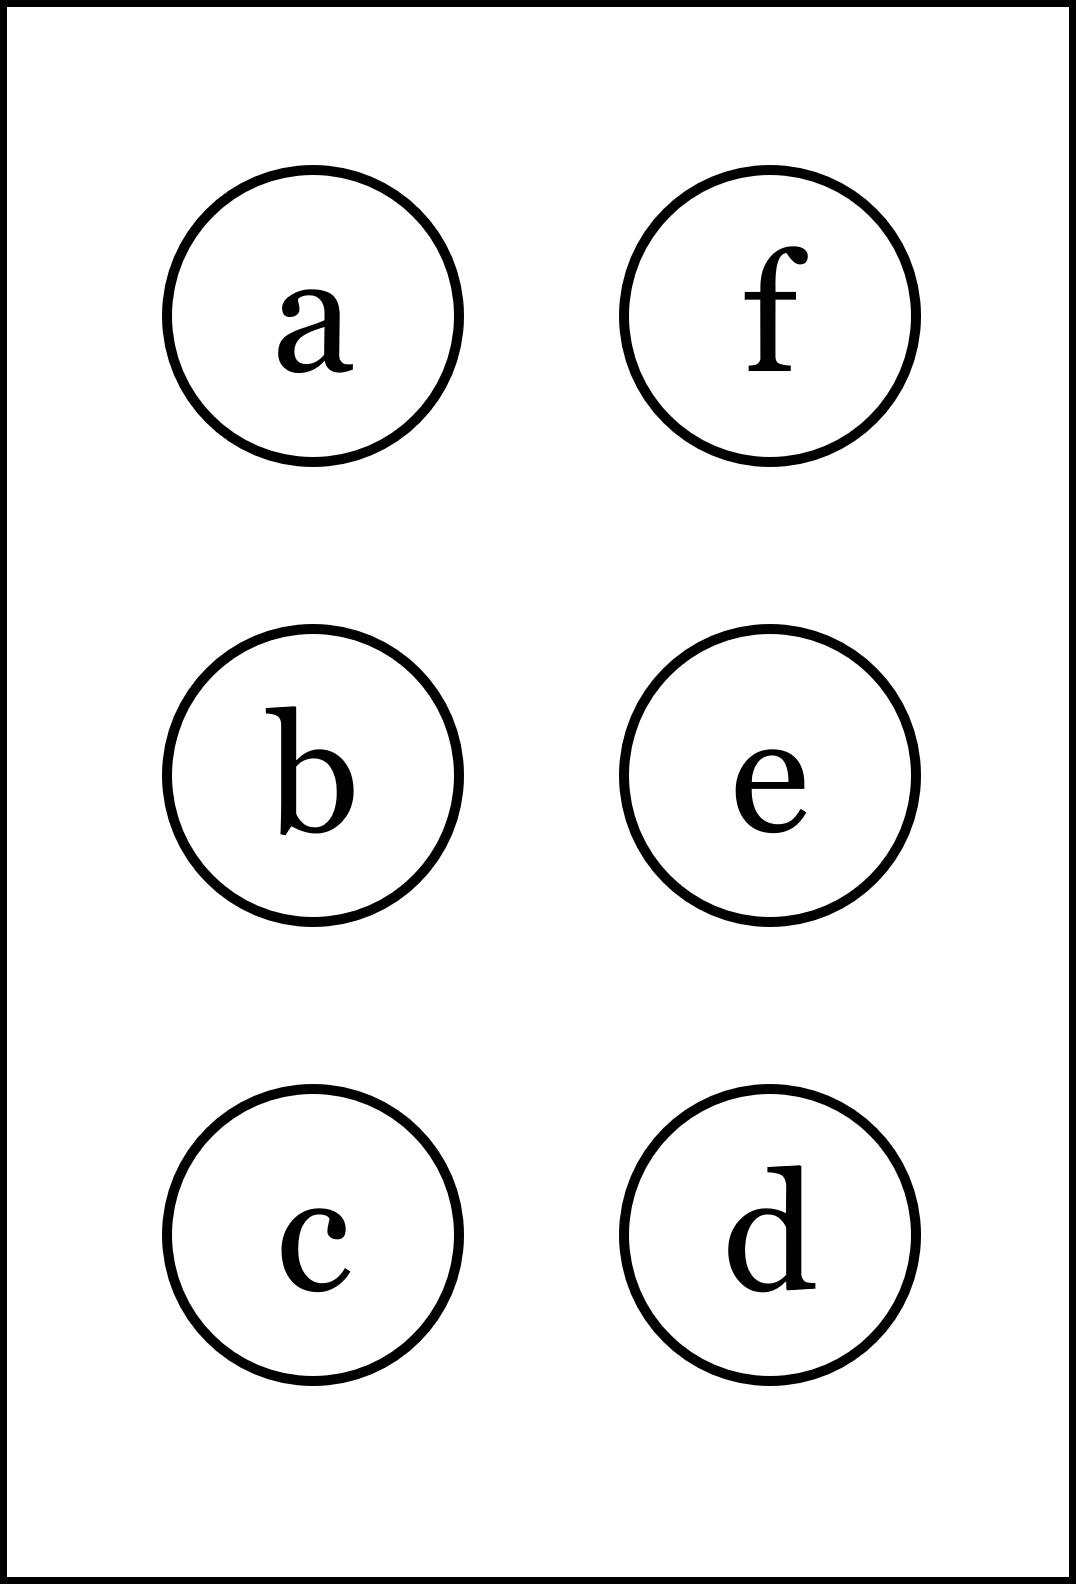
\includegraphics[height=40mm]{../images/braille.png}
{\small Písmeno Braillovej abecedy}
\end{center}
\end{minipage}
\end{center}
\end{minipage}
%
\end{tabular}
\newpage
\thispagestyle{empty}
\begin{tabular}{c:c}
\begin{minipage}[c][104.5mm][t]{0.5\linewidth}
\begin{center}
\vspace{7mm}
{\huge Stacionární body, skupina \textit{Iota $\iota$} -\romannumeral1}\\[5mm]
\textit{Jméno:}\phantom{xxxxxxxxxxxxxxxxxxxxxxxxxxxxxxxxxxxxxxxxxxxxxxxxxxxxxxxxxxxxxxxxx}\\[5mm]
\begin{minipage}{0.95\linewidth}
\begin{center}
{\small V \textbf{(a)} zjisti jestli $f(x)$ \textbf{roste} v bode $x_0$. V \textbf{(b)} zjisti jestli je $f(x)$ v bode $x_0$ \textbf{ryze konvexní}.\\V \textbf{(c)} spočti \textbf{součet} x-ových souřadnic stacionárního a inflexního bodu. V \textbf{(d)} najdi x-ovou souřadnici stacionárního bodu a rozhodli jestli to je \textbf{lomax, lomin či inflex}.\\Pokud se výsledky shodujú s těmi za otazníky, tak napravo obarvi příslušející kroužek načerno.\\\textbf{Spolu odevzdejte výsledné slovo}}.
\end{center}
\end{minipage}
\\[1mm]
\begin{minipage}{0.79\linewidth}
\begin{center}
\begin{varwidth}{\linewidth}
\begin{enumerate}
\normalsize
\item $f(x)=\cfrac{6x^2-4x+5}{-3x-2}\enspace , \enspace x_0=2$\quad \dotfill\; ???\;\dotfill \quad \text{ne}
\item $f(x)=2x^4-5x^3-4x^2-x+2\enspace , \enspace x_0=3$\quad \dotfill\; ???\;\dotfill \quad \text{ano}
\item $f(x)=xe^{x}$\quad \dotfill\; ???\;\dotfill \quad $-3$
\item $f(x)=\sqrt{5x^2-3x+1}$\quad \dotfill\; ???\;\dotfill \quad $\nicefrac{3}{10}\enspace , \enspace\mathrm{lomax}$
\item \quad \dotfill\; ???\;\dotfill \quad nebarvi
\item \quad \dotfill\; ???\;\dotfill \quad nebarvi
\end{enumerate}
\end{varwidth}
\end{center}
\end{minipage}
\begin{minipage}{0.20\linewidth}
\begin{center}
{\Huge\bfseries 1.} \\[2mm]
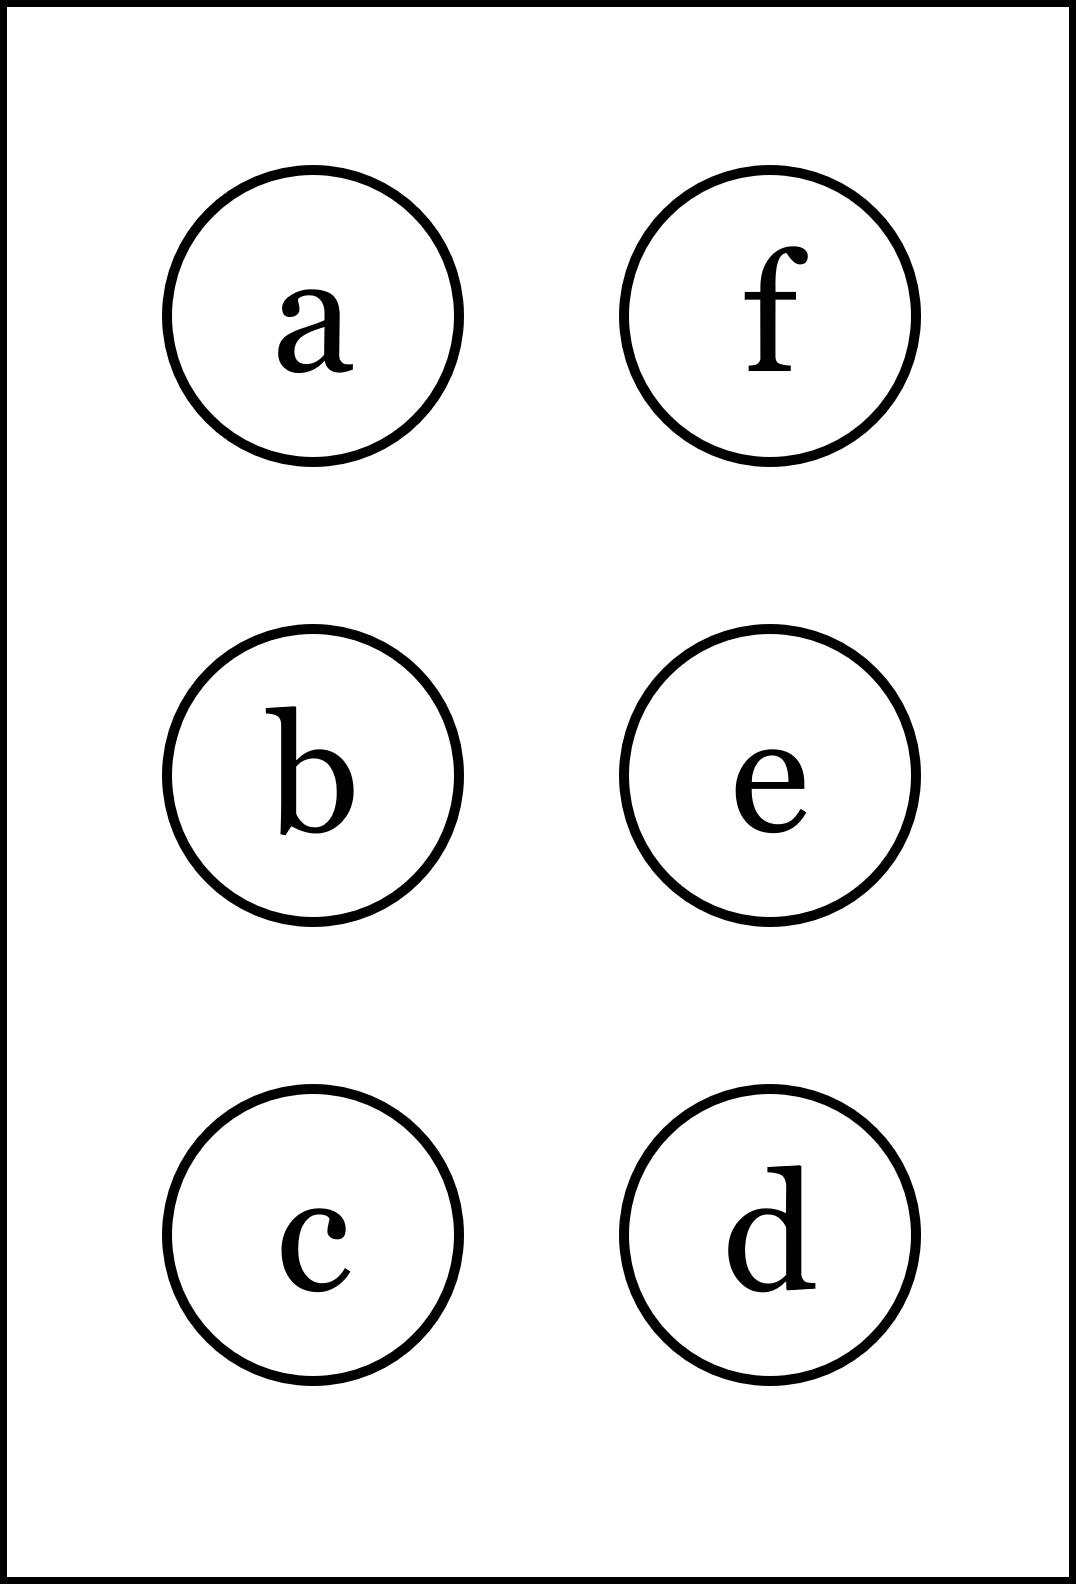
\includegraphics[height=40mm]{../images/braille.png}
{\small Písmeno Braillovej abecedy}
\end{center}
\end{minipage}
\end{center}
\end{minipage}
&
\begin{minipage}[c][104.5mm][t]{0.5\linewidth}
\begin{center}
\vspace{7mm}
{\huge Stacionární body, skupina \textit{Iota $\iota$} -\romannumeral2}\\[5mm]
\textit{Jméno:}\phantom{xxxxxxxxxxxxxxxxxxxxxxxxxxxxxxxxxxxxxxxxxxxxxxxxxxxxxxxxxxxxxxxxx}\\[5mm]
\begin{minipage}{0.95\linewidth}
\begin{center}
{\small V \textbf{(a)} zjisti jestli $f(x)$ \textbf{roste} v bode $x_0$. V \textbf{(b)} zjisti jestli je $f(x)$ v bode $x_0$ \textbf{ryze konvexní}.\\V \textbf{(c)} spočti \textbf{součet} x-ových souřadnic stacionárního a inflexního bodu. V \textbf{(d)} najdi x-ovou souřadnici stacionárního bodu a rozhodli jestli to je \textbf{lomax, lomin či inflex}.\\Pokud se výsledky shodujú s těmi za otazníky, tak napravo obarvi příslušející kroužek načerno.\\\textbf{Spolu odevzdejte výsledné slovo}}.
\end{center}
\end{minipage}
\\[1mm]
\begin{minipage}{0.79\linewidth}
\begin{center}
\begin{varwidth}{\linewidth}
\begin{enumerate}
\normalsize
\item $f(x)=\cfrac{-7x^2+7x-3}{5x+5}\enspace , \enspace x_0=1$\quad \dotfill\; ???\;\dotfill \quad \text{ne}
\item $f(x)=-4x^4-6x^3-6x^2+x-1\enspace , \enspace x_0=-2$\quad \dotfill\; ???\;\dotfill \quad \text{ano}
\item $f(x)=-2xe^{-x}$\quad \dotfill\; ???\;\dotfill \quad $3$
\item $f(x)=\sqrt{3x^2-5x+3}$\quad \dotfill\; ???\;\dotfill \quad $\nicefrac{5}{6}\enspace , \enspace \mathrm{lomin}$
\item \quad \dotfill\; ???\;\dotfill \quad nebarvi
\item \quad \dotfill\; ???\;\dotfill \quad nebarvi
\end{enumerate}
\end{varwidth}
\end{center}
\end{minipage}
\begin{minipage}{0.20\linewidth}
\begin{center}
{\Huge\bfseries 2.} \\[2mm]
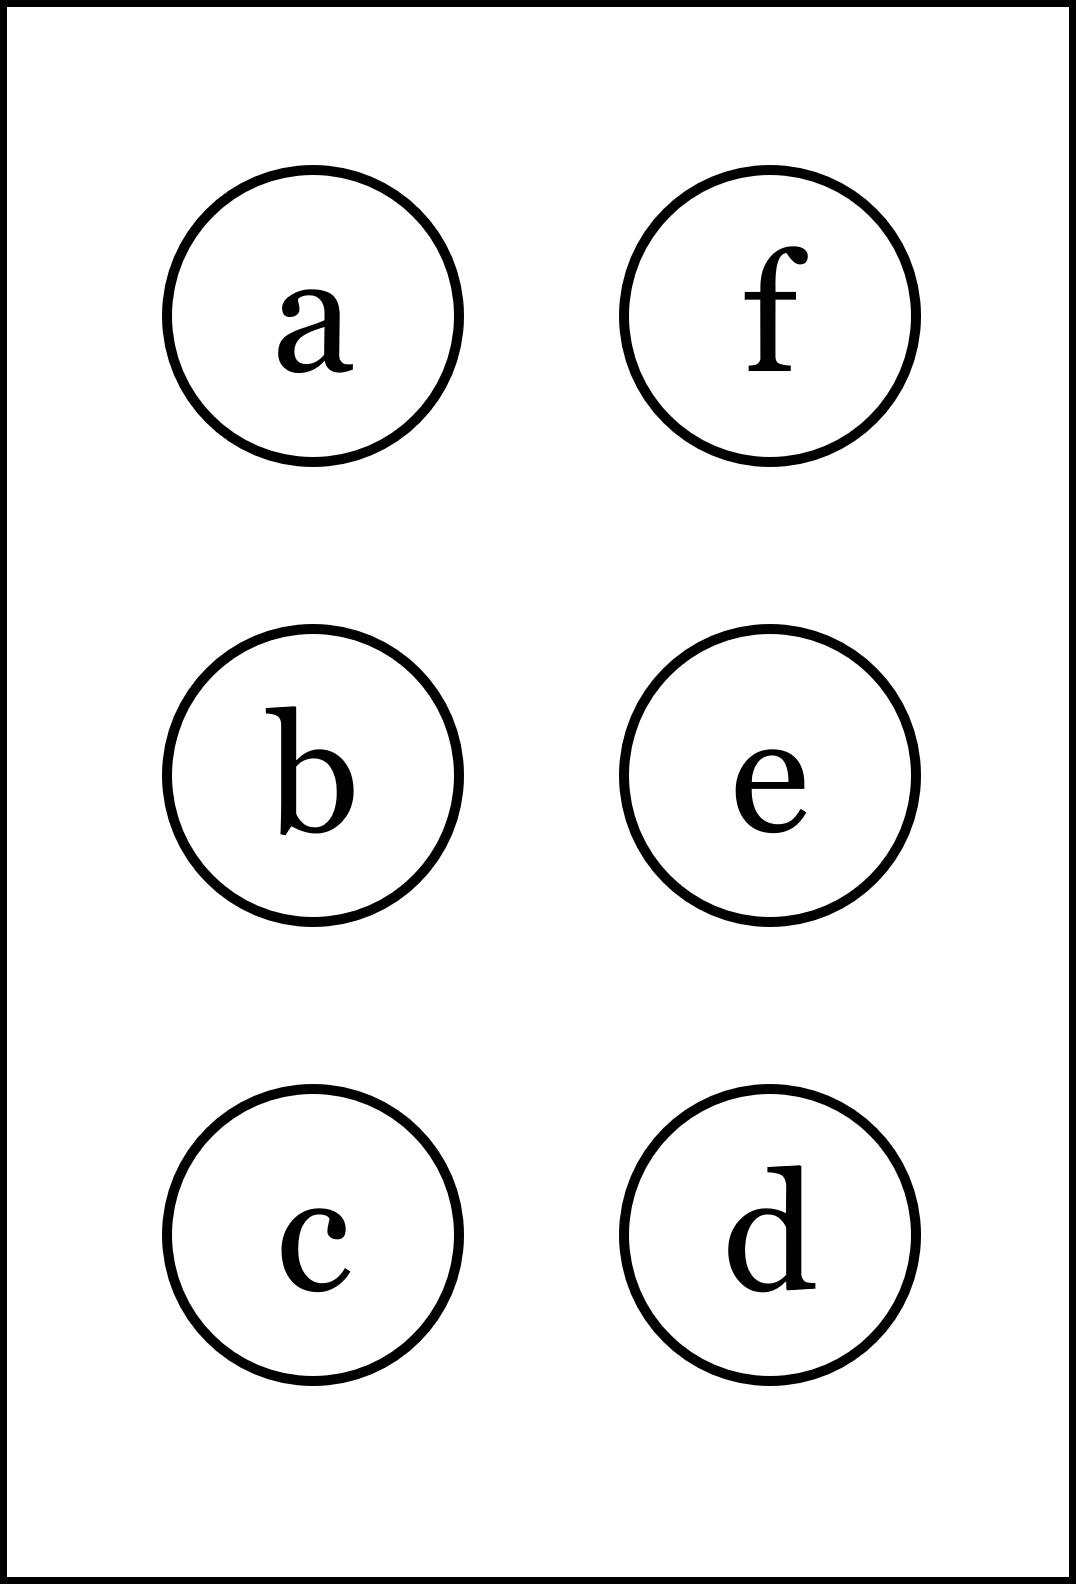
\includegraphics[height=40mm]{../images/braille.png}
{\small Písmeno Braillovej abecedy}
\end{center}
\end{minipage}
\end{center}
\end{minipage}
\\ \hdashline
\begin{minipage}[c][104.5mm][t]{0.5\linewidth}
\begin{center}
\vspace{7mm}
{\huge Stacionární body, skupina \textit{Iota $\iota$} -\romannumeral3}\\[5mm]
\textit{Jméno:}\phantom{xxxxxxxxxxxxxxxxxxxxxxxxxxxxxxxxxxxxxxxxxxxxxxxxxxxxxxxxxxxxxxxxx}\\[5mm]
\begin{minipage}{0.95\linewidth}
\begin{center}
{\small V \textbf{(a)} zjisti jestli $f(x)$ \textbf{roste} v bode $x_0$. V \textbf{(b)} zjisti jestli je $f(x)$ v bode $x_0$ \textbf{ryze konvexní}.\\V \textbf{(c)} spočti \textbf{součet} x-ových souřadnic stacionárního a inflexního bodu. V \textbf{(d)} najdi x-ovou souřadnici stacionárního bodu a rozhodli jestli to je \textbf{lomax, lomin či inflex}.\\Pokud se výsledky shodujú s těmi za otazníky, tak napravo obarvi příslušející kroužek načerno.\\\textbf{Spolu odevzdejte výsledné slovo}}.
\end{center}
\end{minipage}
\\[1mm]
\begin{minipage}{0.79\linewidth}
\begin{center}
\begin{varwidth}{\linewidth}
\begin{enumerate}
\normalsize
\item $f(x)=\cfrac{2x^2-x+1}{-2x+3}\enspace , \enspace x_0=-1$\quad \dotfill\; ???\;\dotfill \quad \text{ne}
\item $f(x)=-x^4-6x^3+4x^2+4x+2\enspace , \enspace x_0=3$\quad \dotfill\; ???\;\dotfill \quad \text{ne}
\item $f(x)=-3xe^{-3x}$\quad \dotfill\; ???\;\dotfill \quad $1$
\item $f(x)=\sqrt{2x^2-2x+1}$\quad \dotfill\; ???\;\dotfill \quad $\nicefrac{1}{2}\enspace , \enspace\mathrm{inflex}$
\item \quad \dotfill\; ???\;\dotfill \quad nebarvi
\item \quad \dotfill\; ???\;\dotfill \quad vybarvi
\end{enumerate}
\end{varwidth}
\end{center}
\end{minipage}
\begin{minipage}{0.20\linewidth}
\begin{center}
{\Huge\bfseries 3.} \\[2mm]
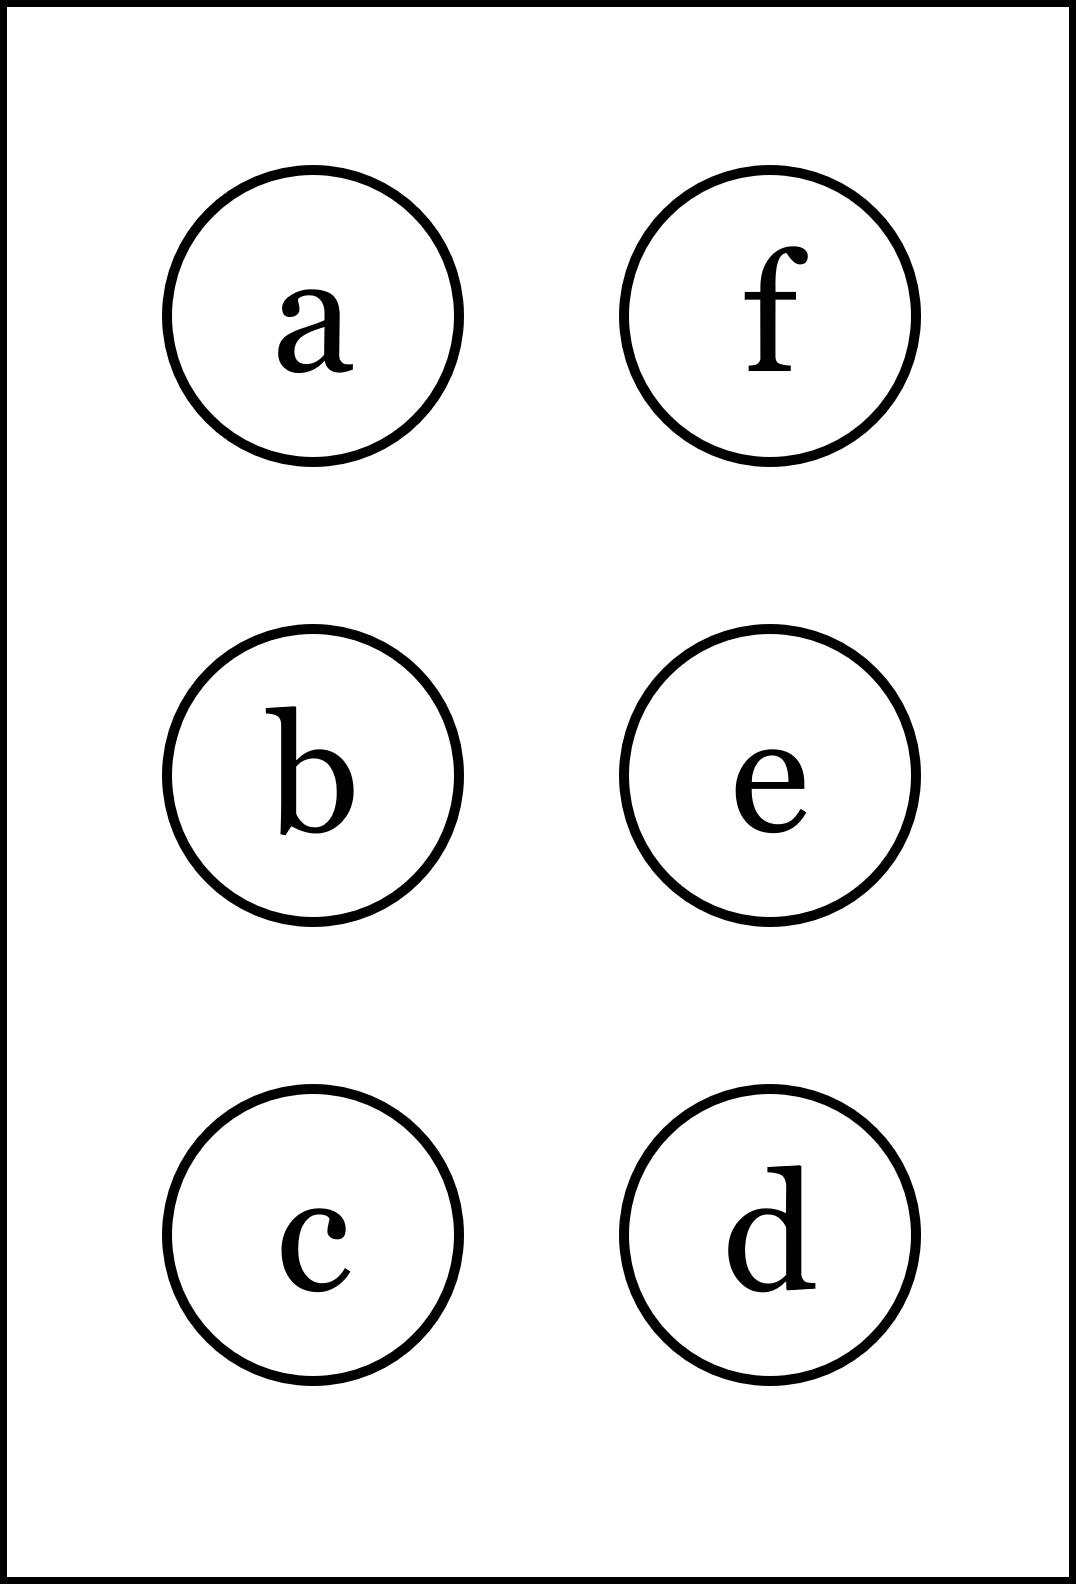
\includegraphics[height=40mm]{../images/braille.png}
{\small Písmeno Braillovej abecedy}
\end{center}
\end{minipage}
\end{center}
\end{minipage}
&
\begin{minipage}[c][104.5mm][t]{0.5\linewidth}
\begin{center}
\vspace{7mm}
{\huge Stacionární body, skupina \textit{Iota $\iota$} -\romannumeral4}\\[5mm]
\textit{Jméno:}\phantom{xxxxxxxxxxxxxxxxxxxxxxxxxxxxxxxxxxxxxxxxxxxxxxxxxxxxxxxxxxxxxxxxx}\\[5mm]
\begin{minipage}{0.95\linewidth}
\begin{center}
{\small V \textbf{(a)} zjisti jestli $f(x)$ \textbf{roste} v bode $x_0$. V \textbf{(b)} zjisti jestli je $f(x)$ v bode $x_0$ \textbf{ryze konvexní}.\\V \textbf{(c)} spočti \textbf{součet} x-ových souřadnic stacionárního a inflexního bodu. V \textbf{(d)} najdi x-ovou souřadnici stacionárního bodu a rozhodli jestli to je \textbf{lomax, lomin či inflex}.\\Pokud se výsledky shodujú s těmi za otazníky, tak napravo obarvi příslušející kroužek načerno.\\\textbf{Spolu odevzdejte výsledné slovo}}.
\end{center}
\end{minipage}
\\[1mm]
\begin{minipage}{0.79\linewidth}
\begin{center}
\begin{varwidth}{\linewidth}
\begin{enumerate}
\normalsize
\item $f(x)=\cfrac{-x^2-3x-2}{-2x+2}\enspace , \enspace x_0=-3$\quad \dotfill\; ???\;\dotfill \quad \text{ano}
\item $f(x)=9x^4+x^3+2x^2+4x-7\enspace , \enspace x_0=2$\quad \dotfill\; ???\;\dotfill \quad \text{ne}
\item $f(x)=-2xe^{-3x}$\quad \dotfill\; ???\;\dotfill \quad $\nicefrac{-1}{3}$
\item $f(x)=\sqrt{3x^2+x+1}$\quad \dotfill\; ???\;\dotfill \quad $\nicefrac{-1}{6}\enspace , \enspace\mathrm{lomax}$
\item \quad \dotfill\; ???\;\dotfill \quad nebarvi
\item \quad \dotfill\; ???\;\dotfill \quad nebarvi
\end{enumerate}
\end{varwidth}
\end{center}
\end{minipage}
\begin{minipage}{0.20\linewidth}
\begin{center}
{\Huge\bfseries 4.} \\[2mm]
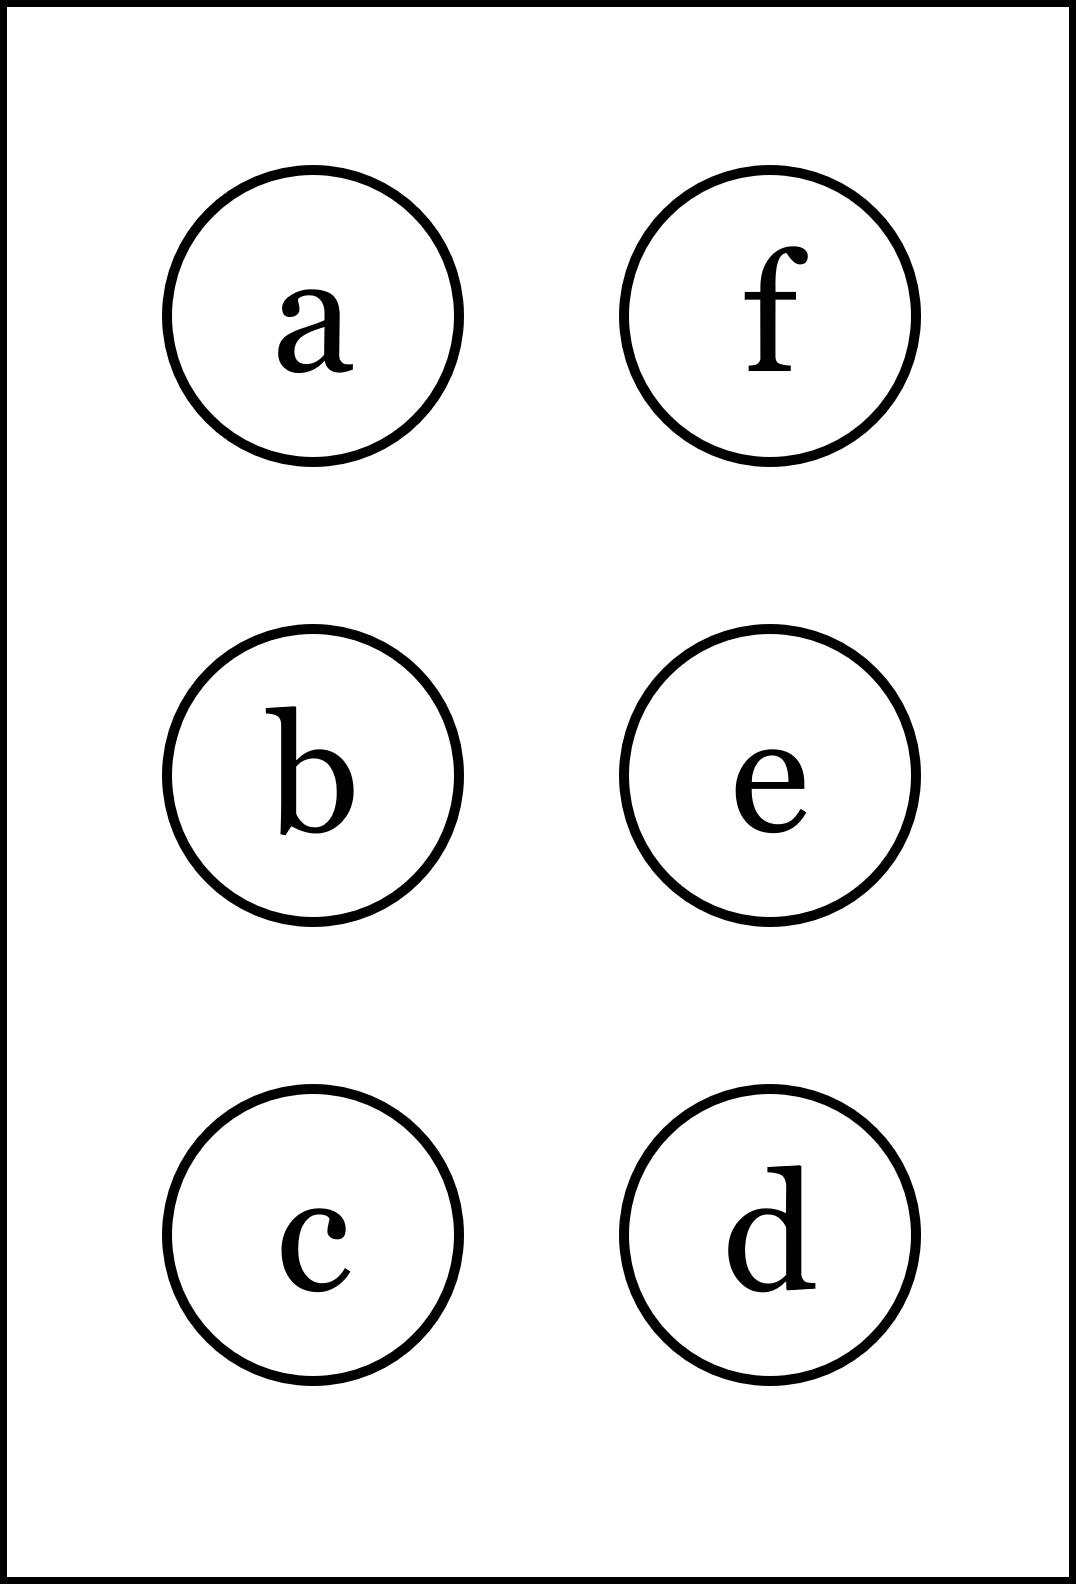
\includegraphics[height=40mm]{../images/braille.png}
{\small Písmeno Braillovej abecedy}
\end{center}
\end{minipage}
\end{center}
\end{minipage}
%
\end{tabular}
\newpage
\thispagestyle{empty}
\begin{tabular}{c:c}
\begin{minipage}[c][104.5mm][t]{0.5\linewidth}
\begin{center}
\vspace{7mm}
{\huge Stacionární body, skupina \textit{Kappa $\kappa$} -\romannumeral1}\\[5mm]
\textit{Jméno:}\phantom{xxxxxxxxxxxxxxxxxxxxxxxxxxxxxxxxxxxxxxxxxxxxxxxxxxxxxxxxxxxxxxxxx}\\[5mm]
\begin{minipage}{0.95\linewidth}
\begin{center}
{\small V \textbf{(a)} zjisti jestli $f(x)$ \textbf{roste} v bode $x_0$. V \textbf{(b)} zjisti jestli je $f(x)$ v bode $x_0$ \textbf{ryze konvexní}.\\V \textbf{(c)} spočti \textbf{součet} x-ových souřadnic stacionárního a inflexního bodu. V \textbf{(d)} najdi x-ovou souřadnici stacionárního bodu a rozhodli jestli to je \textbf{lomax, lomin či inflex}.\\Pokud se výsledky shodujú s těmi za otazníky, tak napravo obarvi příslušející kroužek načerno.\\\textbf{Spolu odevzdejte výsledné slovo}}.
\end{center}
\end{minipage}
\\[1mm]
\begin{minipage}{0.79\linewidth}
\begin{center}
\begin{varwidth}{\linewidth}
\begin{enumerate}
\normalsize
\item $f(x)=\cfrac{3x^2+5x-4}{3x+7}\enspace , \enspace x_0=1$\quad \dotfill\; ???\;\dotfill \quad \text{ano}
\item $f(x)=-5x^4-8x^3-5x^2+5x+4\enspace , \enspace x_0=-1$\quad \dotfill\; ???\;\dotfill \quad \text{ano}
\item $f(x)=-7xe^{5x}$\quad \dotfill\; ???\;\dotfill \quad $\nicefrac{-3}{5}$
\item $f(x)=\sqrt{2x^2+x+1}$\quad \dotfill\; ???\;\dotfill \quad $\nicefrac{-1}{4}\enspace , \enspace \mathrm{lomin}$
\item \quad \dotfill\; ???\;\dotfill \quad vybarvi
\item \quad \dotfill\; ???\;\dotfill \quad nebarvi
\end{enumerate}
\end{varwidth}
\end{center}
\end{minipage}
\begin{minipage}{0.20\linewidth}
\begin{center}
{\Huge\bfseries 1.} \\[2mm]
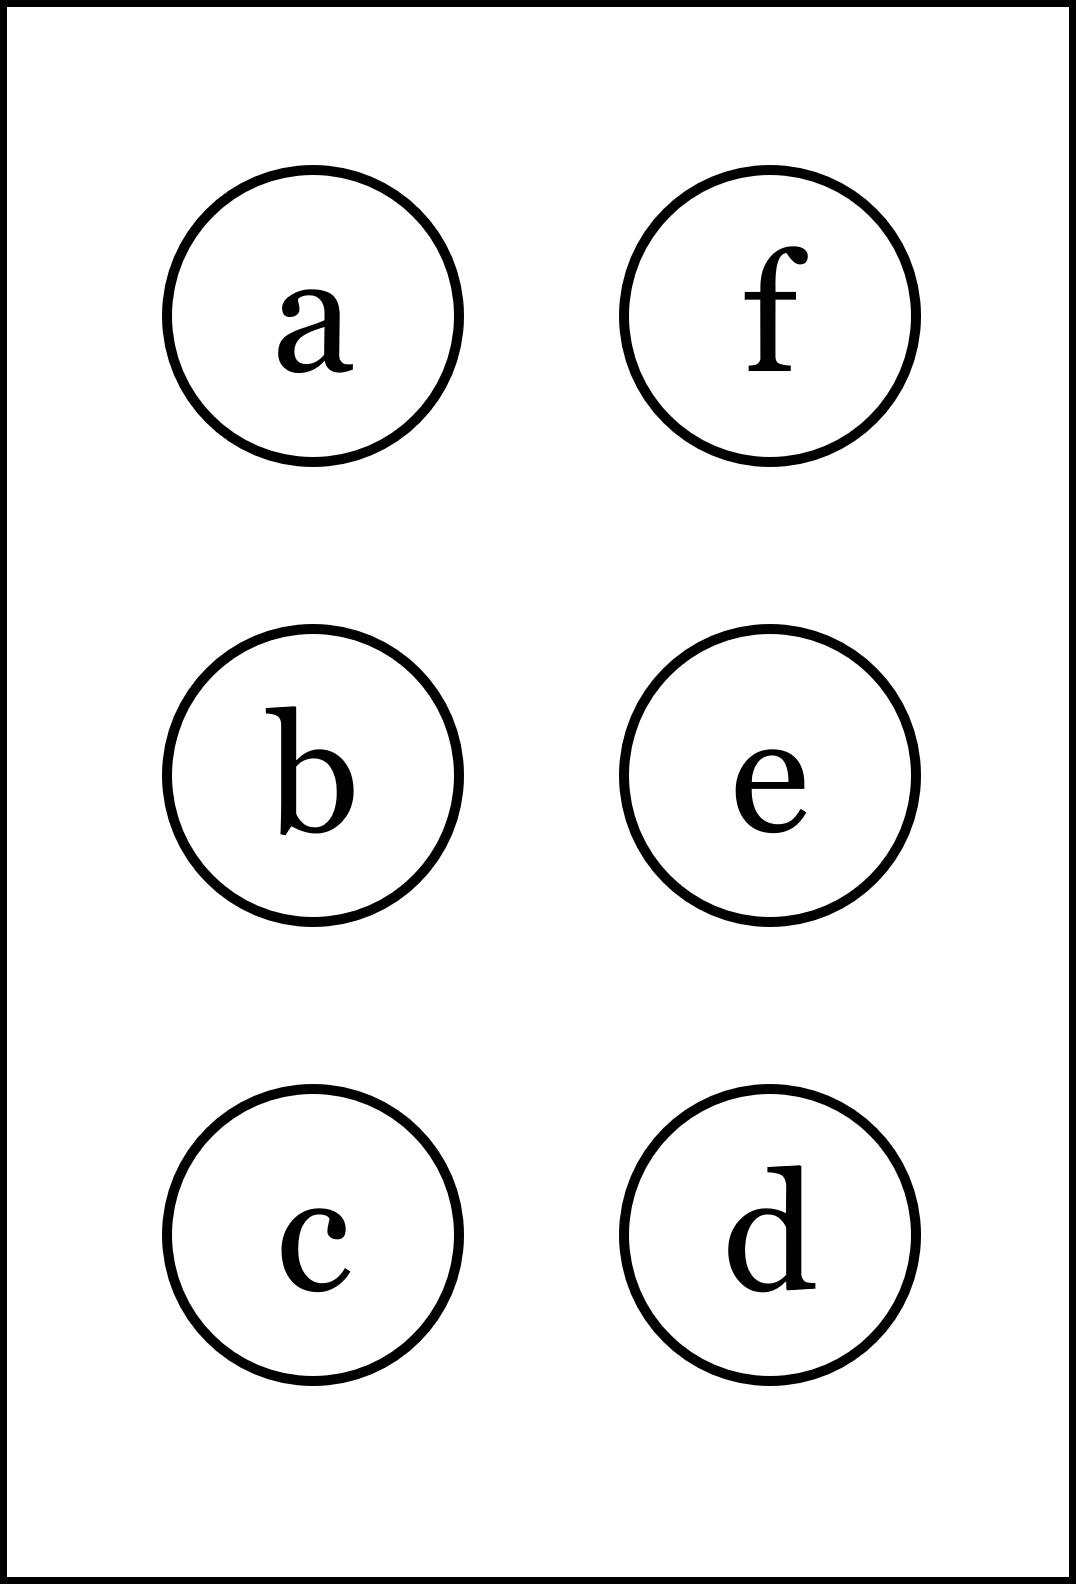
\includegraphics[height=40mm]{../images/braille.png}
{\small Písmeno Braillovej abecedy}
\end{center}
\end{minipage}
\end{center}
\end{minipage}
&
\begin{minipage}[c][104.5mm][t]{0.5\linewidth}
\begin{center}
\vspace{7mm}
{\huge Stacionární body, skupina \textit{Kappa $\kappa$} -\romannumeral2}\\[5mm]
\textit{Jméno:}\phantom{xxxxxxxxxxxxxxxxxxxxxxxxxxxxxxxxxxxxxxxxxxxxxxxxxxxxxxxxxxxxxxxxx}\\[5mm]
\begin{minipage}{0.95\linewidth}
\begin{center}
{\small V \textbf{(a)} zjisti jestli $f(x)$ \textbf{roste} v bode $x_0$. V \textbf{(b)} zjisti jestli je $f(x)$ v bode $x_0$ \textbf{ryze konvexní}.\\V \textbf{(c)} spočti \textbf{součet} x-ových souřadnic stacionárního a inflexního bodu. V \textbf{(d)} najdi x-ovou souřadnici stacionárního bodu a rozhodli jestli to je \textbf{lomax, lomin či inflex}.\\Pokud se výsledky shodujú s těmi za otazníky, tak napravo obarvi příslušející kroužek načerno.\\\textbf{Spolu odevzdejte výsledné slovo}}.
\end{center}
\end{minipage}
\\[1mm]
\begin{minipage}{0.79\linewidth}
\begin{center}
\begin{varwidth}{\linewidth}
\begin{enumerate}
\normalsize
\item $f(x)=\cfrac{-2x^2+5x-5}{-2x+5}\enspace , \enspace x_0=1$\quad \dotfill\; ???\;\dotfill \quad \text{ne}
\item $f(x)=x^4+x^3+5x^2-4x-6\enspace , \enspace x_0=2$\quad \dotfill\; ???\;\dotfill \quad \text{ne}
\item $f(x)=xe^{-x}$\quad \dotfill\; ???\;\dotfill \quad $3$
\item $f(x)=\sqrt{2x^2-4x+3}$\quad \dotfill\; ???\;\dotfill \quad $1\enspace , \enspace \mathrm{lomin}$
\item \quad \dotfill\; ???\;\dotfill \quad nebarvi
\item \quad \dotfill\; ???\;\dotfill \quad nebarvi
\end{enumerate}
\end{varwidth}
\end{center}
\end{minipage}
\begin{minipage}{0.20\linewidth}
\begin{center}
{\Huge\bfseries 2.} \\[2mm]
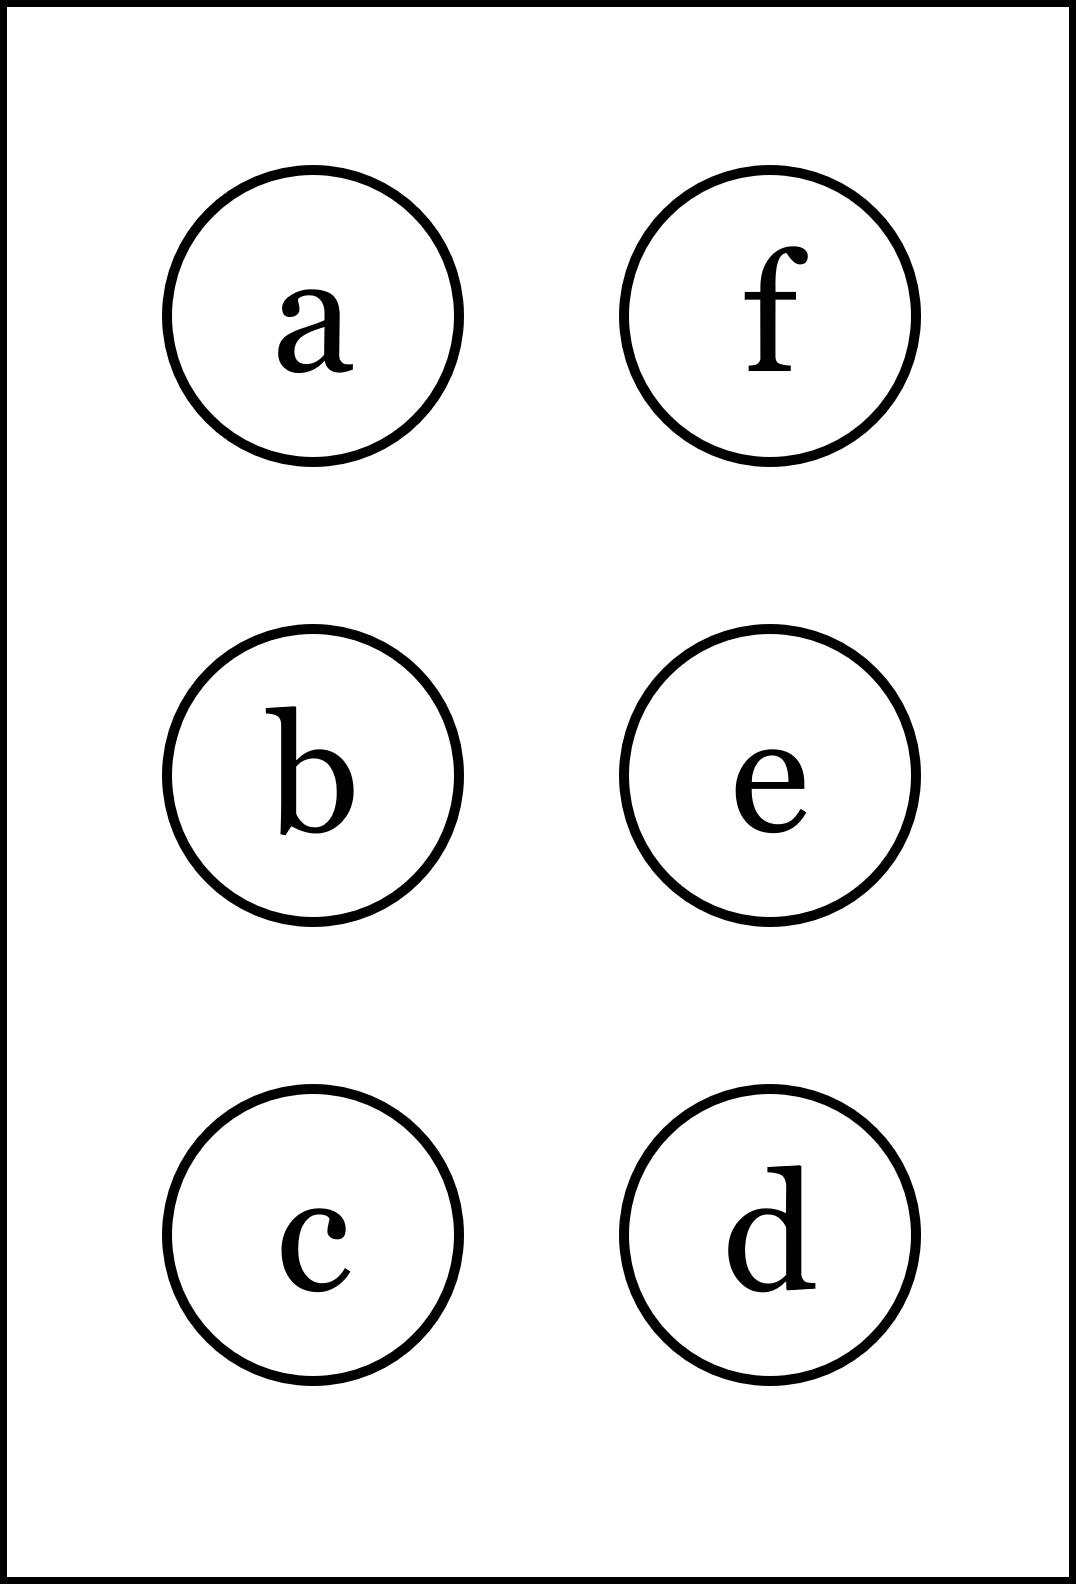
\includegraphics[height=40mm]{../images/braille.png}
{\small Písmeno Braillovej abecedy}
\end{center}
\end{minipage}
\end{center}
\end{minipage}
\\ \hdashline
\begin{minipage}[c][104.5mm][t]{0.5\linewidth}
\begin{center}
\vspace{7mm}
{\huge Stacionární body, skupina \textit{Kappa $\kappa$} -\romannumeral3}\\[5mm]
\textit{Jméno:}\phantom{xxxxxxxxxxxxxxxxxxxxxxxxxxxxxxxxxxxxxxxxxxxxxxxxxxxxxxxxxxxxxxxxx}\\[5mm]
\begin{minipage}{0.95\linewidth}
\begin{center}
{\small V \textbf{(a)} zjisti jestli $f(x)$ \textbf{roste} v bode $x_0$. V \textbf{(b)} zjisti jestli je $f(x)$ v bode $x_0$ \textbf{ryze konvexní}.\\V \textbf{(c)} spočti \textbf{součet} x-ových souřadnic stacionárního a inflexního bodu. V \textbf{(d)} najdi x-ovou souřadnici stacionárního bodu a rozhodli jestli to je \textbf{lomax, lomin či inflex}.\\Pokud se výsledky shodujú s těmi za otazníky, tak napravo obarvi příslušející kroužek načerno.\\\textbf{Spolu odevzdejte výsledné slovo}}.
\end{center}
\end{minipage}
\\[1mm]
\begin{minipage}{0.79\linewidth}
\begin{center}
\begin{varwidth}{\linewidth}
\begin{enumerate}
\normalsize
\item $f(x)=\cfrac{-3x^2+5x-7}{3x+3}\enspace , \enspace x_0=-2$\quad \dotfill\; ???\;\dotfill \quad \text{ano}
\item $f(x)=-x^4+2x^3+5x^2+3x-7\enspace , \enspace x_0=-2$\quad \dotfill\; ???\;\dotfill \quad \text{ne}
\item $f(x)=-3xe^{-x}$\quad \dotfill\; ???\;\dotfill \quad $-1$
\item $f(x)=\sqrt{2x^2+3x+4}$\quad \dotfill\; ???\;\dotfill \quad $\nicefrac{-3}{4}\enspace , \enspace\mathrm{lomax}$
\item \quad \dotfill\; ???\;\dotfill \quad nebarvi
\item \quad \dotfill\; ???\;\dotfill \quad nebarvi
\end{enumerate}
\end{varwidth}
\end{center}
\end{minipage}
\begin{minipage}{0.20\linewidth}
\begin{center}
{\Huge\bfseries 3.} \\[2mm]
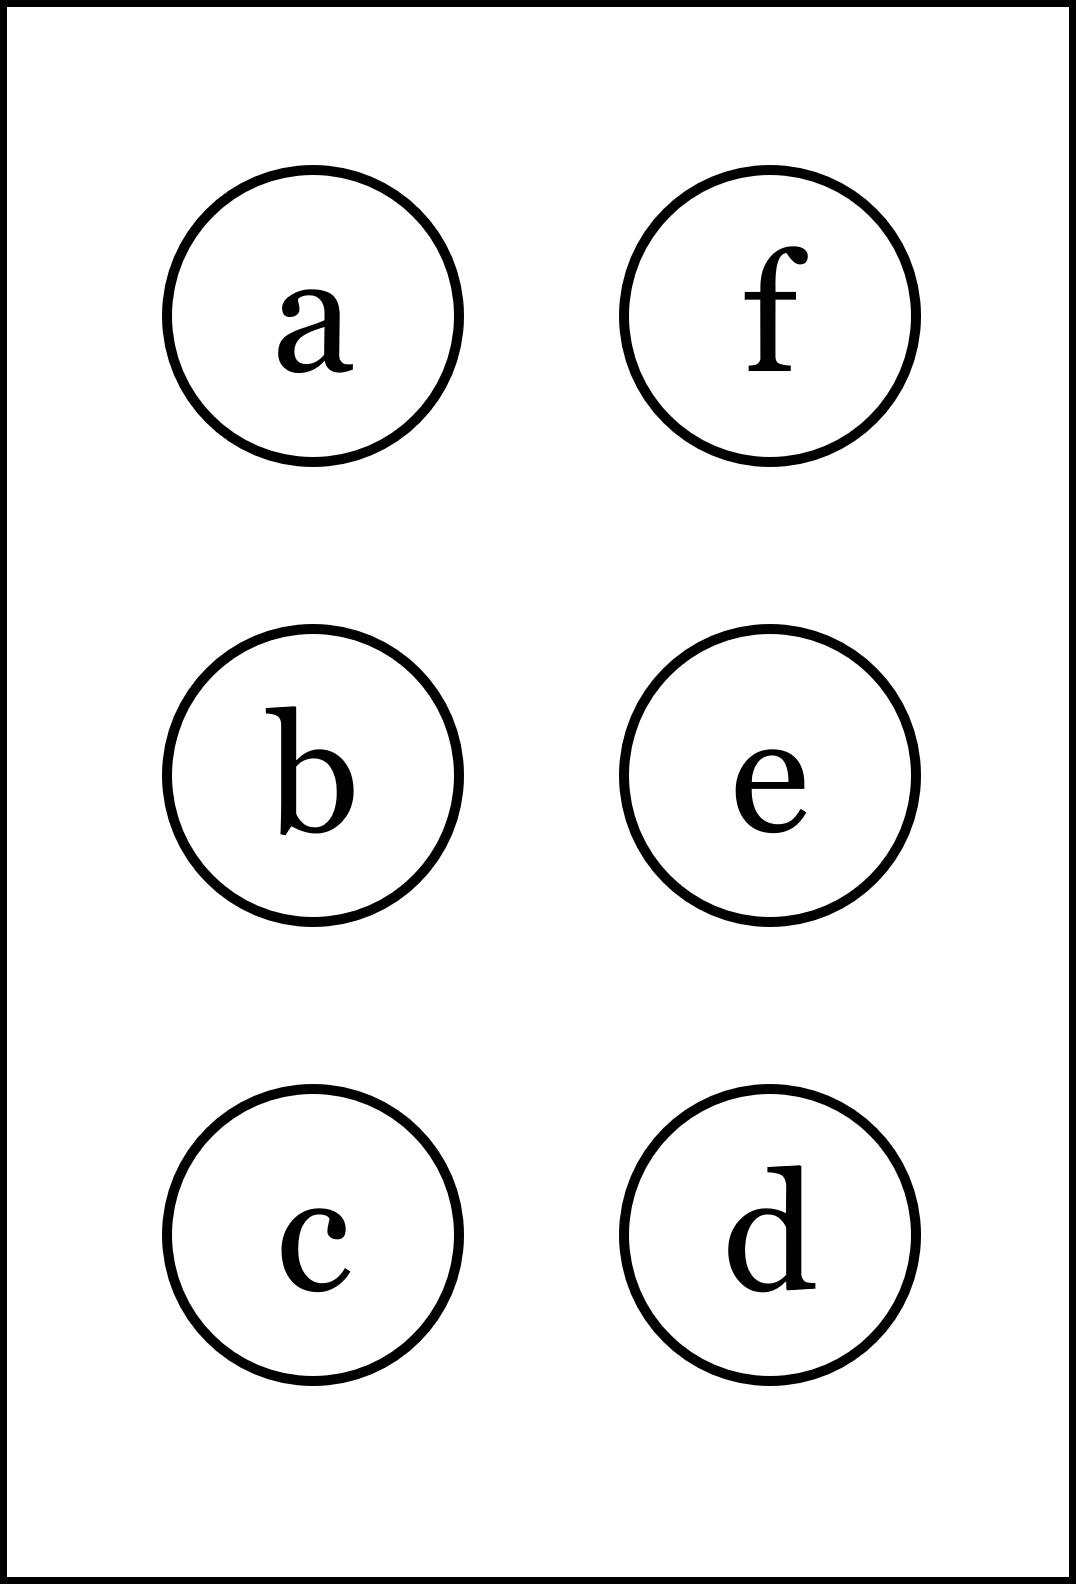
\includegraphics[height=40mm]{../images/braille.png}
{\small Písmeno Braillovej abecedy}
\end{center}
\end{minipage}
\end{center}
\end{minipage}
&
\begin{minipage}[c][104.5mm][t]{0.5\linewidth}
\begin{center}
\vspace{7mm}
{\huge Stacionární body, skupina \textit{Kappa $\kappa$} -\romannumeral4}\\[5mm]
\textit{Jméno:}\phantom{xxxxxxxxxxxxxxxxxxxxxxxxxxxxxxxxxxxxxxxxxxxxxxxxxxxxxxxxxxxxxxxxx}\\[5mm]
\begin{minipage}{0.95\linewidth}
\begin{center}
{\small V \textbf{(a)} zjisti jestli $f(x)$ \textbf{roste} v bode $x_0$. V \textbf{(b)} zjisti jestli je $f(x)$ v bode $x_0$ \textbf{ryze konvexní}.\\V \textbf{(c)} spočti \textbf{součet} x-ových souřadnic stacionárního a inflexního bodu. V \textbf{(d)} najdi x-ovou souřadnici stacionárního bodu a rozhodli jestli to je \textbf{lomax, lomin či inflex}.\\Pokud se výsledky shodujú s těmi za otazníky, tak napravo obarvi příslušející kroužek načerno.\\\textbf{Spolu odevzdejte výsledné slovo}}.
\end{center}
\end{minipage}
\\[1mm]
\begin{minipage}{0.79\linewidth}
\begin{center}
\begin{varwidth}{\linewidth}
\begin{enumerate}
\normalsize
\item $f(x)=\cfrac{5x^2+3x+1}{-x+5}\enspace , \enspace x_0=2$\quad \dotfill\; ???\;\dotfill \quad \text{ano}
\item $f(x)=-6x^4+5x^3-6x^2-x-3\enspace , \enspace x_0=1$\quad \dotfill\; ???\;\dotfill \quad \text{ne}
\item $f(x)=-2xe^{4x}$\quad \dotfill\; ???\;\dotfill \quad $\nicefrac{-3}{4}$
\item $f(x)=\sqrt{2x^2+x+1}$\quad \dotfill\; ???\;\dotfill \quad $\nicefrac{-1}{4}\enspace , \enspace\mathrm{inflex}$
\item \quad \dotfill\; ???\;\dotfill \quad vybarvi
\item \quad \dotfill\; ???\;\dotfill \quad nebarvi
\end{enumerate}
\end{varwidth}
\end{center}
\end{minipage}
\begin{minipage}{0.20\linewidth}
\begin{center}
{\Huge\bfseries 4.} \\[2mm]
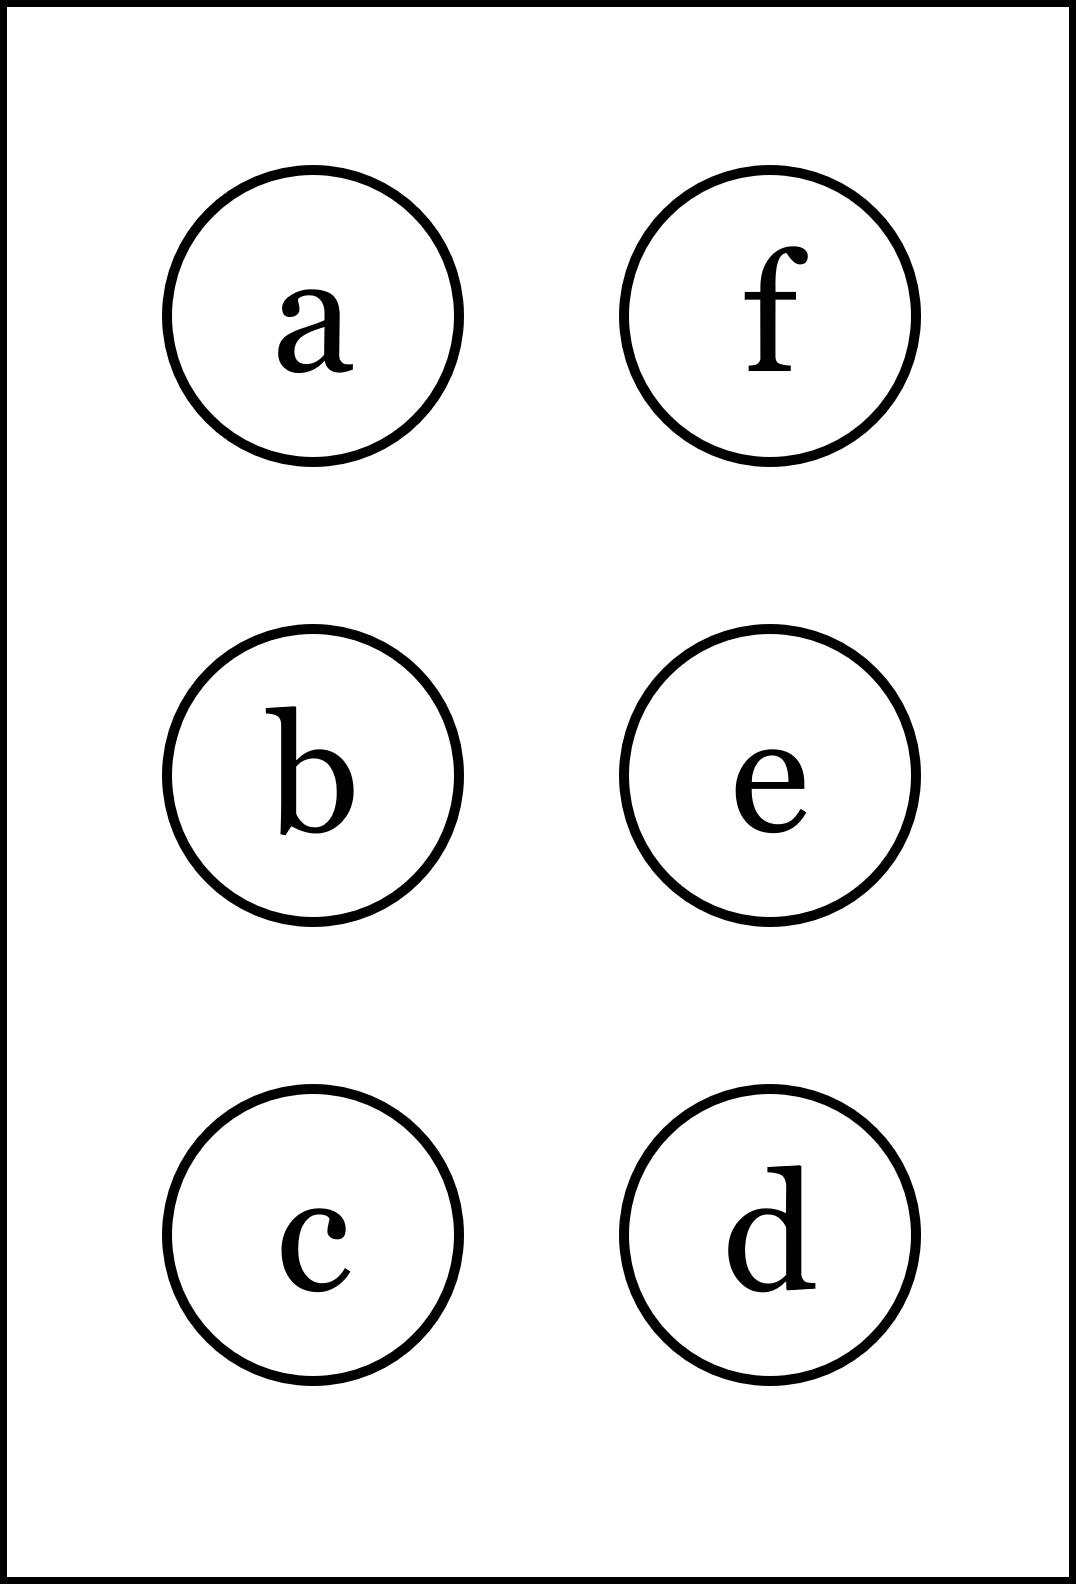
\includegraphics[height=40mm]{../images/braille.png}
{\small Písmeno Braillovej abecedy}
\end{center}
\end{minipage}
\end{center}
\end{minipage}
%
\end{tabular}
\newpage
\thispagestyle{empty}
\begin{tabular}{c:c}
\begin{minipage}[c][104.5mm][t]{0.5\linewidth}
\begin{center}
\vspace{7mm}
{\huge Stacionární body, skupina \textit{Lambda $\lambda$} -\romannumeral1}\\[5mm]
\textit{Jméno:}\phantom{xxxxxxxxxxxxxxxxxxxxxxxxxxxxxxxxxxxxxxxxxxxxxxxxxxxxxxxxxxxxxxxxx}\\[5mm]
\begin{minipage}{0.95\linewidth}
\begin{center}
{\small V \textbf{(a)} zjisti jestli $f(x)$ \textbf{roste} v bode $x_0$. V \textbf{(b)} zjisti jestli je $f(x)$ v bode $x_0$ \textbf{ryze konvexní}.\\V \textbf{(c)} spočti \textbf{součet} x-ových souřadnic stacionárního a inflexního bodu. V \textbf{(d)} najdi x-ovou souřadnici stacionárního bodu a rozhodli jestli to je \textbf{lomax, lomin či inflex}.\\Pokud se výsledky shodujú s těmi za otazníky, tak napravo obarvi příslušející kroužek načerno.\\\textbf{Spolu odevzdejte výsledné slovo}}.
\end{center}
\end{minipage}
\\[1mm]
\begin{minipage}{0.79\linewidth}
\begin{center}
\begin{varwidth}{\linewidth}
\begin{enumerate}
\normalsize
\item $f(x)=\cfrac{-2x^2+9x+4}{x+1}\enspace , \enspace x_0=5$\quad \dotfill\; ???\;\dotfill \quad \text{ne}
\item $f(x)=3x^4-2x^3+7x^2-8x-5\enspace , \enspace x_0=-2$\quad \dotfill\; ???\;\dotfill \quad \text{ne}
\item $f(x)=xe^{-4x}$\quad \dotfill\; ???\;\dotfill \quad $\nicefrac{-1}{4}$
\item $f(x)=\sqrt{x^2+x+4}$\quad \dotfill\; ???\;\dotfill \quad $\nicefrac{-1}{2}\enspace , \enspace\mathrm{lomax}$
\item \quad \dotfill\; ???\;\dotfill \quad vybarvi
\item \quad \dotfill\; ???\;\dotfill \quad vybarvi
\end{enumerate}
\end{varwidth}
\end{center}
\end{minipage}
\begin{minipage}{0.20\linewidth}
\begin{center}
{\Huge\bfseries 1.} \\[2mm]
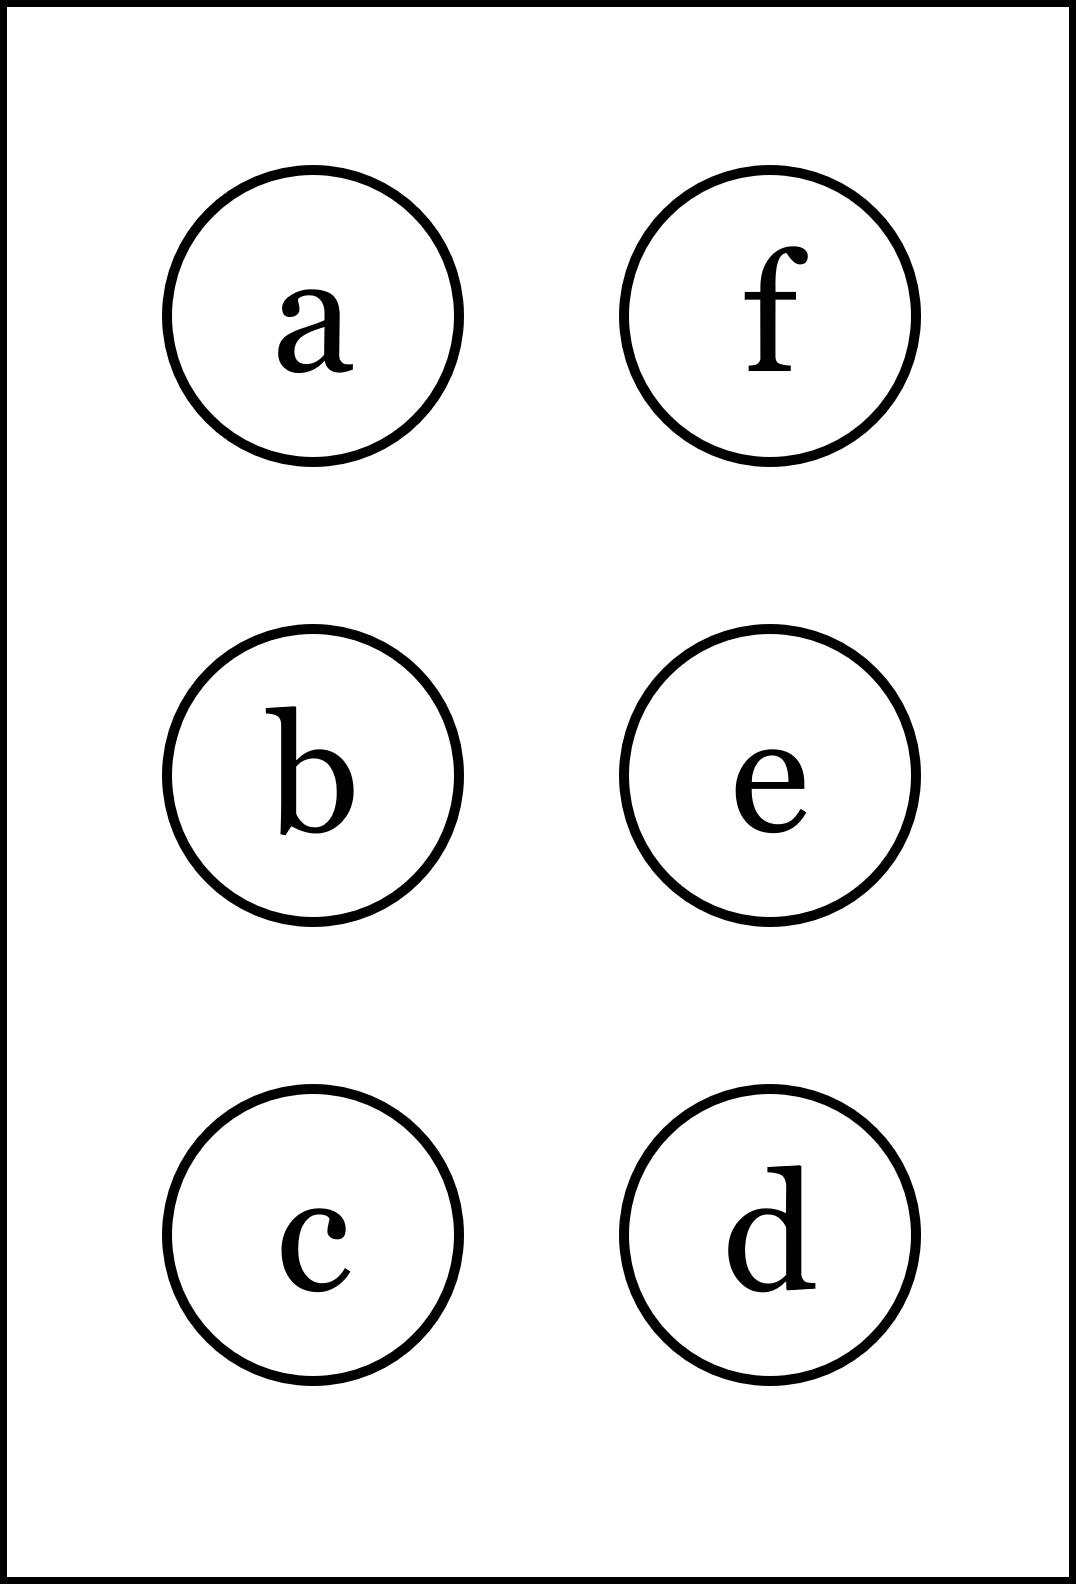
\includegraphics[height=40mm]{../images/braille.png}
{\small Písmeno Braillovej abecedy}
\end{center}
\end{minipage}
\end{center}
\end{minipage}
&
\begin{minipage}[c][104.5mm][t]{0.5\linewidth}
\begin{center}
\vspace{7mm}
{\huge Stacionární body, skupina \textit{Lambda $\lambda$} -\romannumeral2}\\[5mm]
\textit{Jméno:}\phantom{xxxxxxxxxxxxxxxxxxxxxxxxxxxxxxxxxxxxxxxxxxxxxxxxxxxxxxxxxxxxxxxxx}\\[5mm]
\begin{minipage}{0.95\linewidth}
\begin{center}
{\small V \textbf{(a)} zjisti jestli $f(x)$ \textbf{roste} v bode $x_0$. V \textbf{(b)} zjisti jestli je $f(x)$ v bode $x_0$ \textbf{ryze konvexní}.\\V \textbf{(c)} spočti \textbf{součet} x-ových souřadnic stacionárního a inflexního bodu. V \textbf{(d)} najdi x-ovou souřadnici stacionárního bodu a rozhodli jestli to je \textbf{lomax, lomin či inflex}.\\Pokud se výsledky shodujú s těmi za otazníky, tak napravo obarvi příslušející kroužek načerno.\\\textbf{Spolu odevzdejte výsledné slovo}}.
\end{center}
\end{minipage}
\\[1mm]
\begin{minipage}{0.79\linewidth}
\begin{center}
\begin{varwidth}{\linewidth}
\begin{enumerate}
\normalsize
\item $f(x)=\cfrac{-4x^2-3x-2}{5x+3}\enspace , \enspace x_0=1$\quad \dotfill\; ???\;\dotfill \quad \text{ne}
\item $f(x)=7x^4+x^3-x^2-4x-3\enspace , \enspace x_0=-1$\quad \dotfill\; ???\;\dotfill \quad \text{ne}
\item $f(x)=2xe^{-2x}$\quad \dotfill\; ???\;\dotfill \quad $\nicefrac{3}{2}$
\item $f(x)=\sqrt{3x^2+4x+2}$\quad \dotfill\; ???\;\dotfill \quad $\nicefrac{-2}{3}\enspace , \enspace\mathrm{lomax}$
\item \quad \dotfill\; ???\;\dotfill \quad vybarvi
\item \quad \dotfill\; ???\;\dotfill \quad nebarvi
\end{enumerate}
\end{varwidth}
\end{center}
\end{minipage}
\begin{minipage}{0.20\linewidth}
\begin{center}
{\Huge\bfseries 2.} \\[2mm]
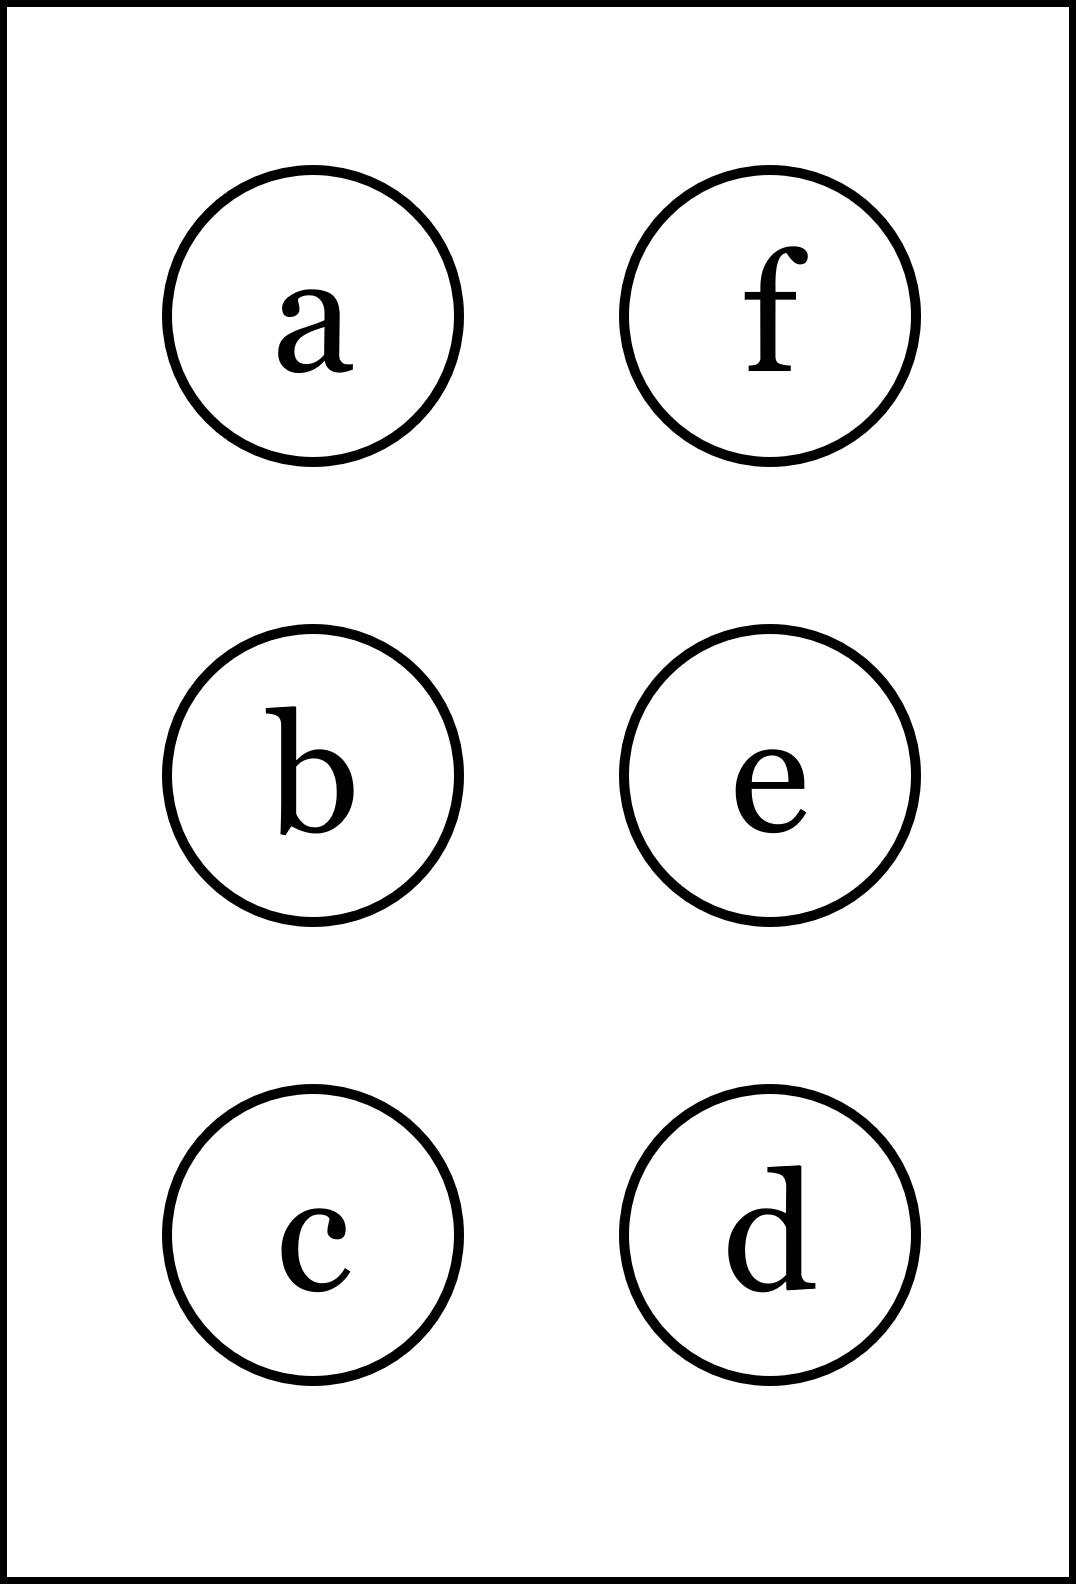
\includegraphics[height=40mm]{../images/braille.png}
{\small Písmeno Braillovej abecedy}
\end{center}
\end{minipage}
\end{center}
\end{minipage}
\\ \hdashline
\begin{minipage}[c][104.5mm][t]{0.5\linewidth}
\begin{center}
\vspace{7mm}
{\huge Stacionární body, skupina \textit{Lambda $\lambda$} -\romannumeral3}\\[5mm]
\textit{Jméno:}\phantom{xxxxxxxxxxxxxxxxxxxxxxxxxxxxxxxxxxxxxxxxxxxxxxxxxxxxxxxxxxxxxxxxx}\\[5mm]
\begin{minipage}{0.95\linewidth}
\begin{center}
{\small V \textbf{(a)} zjisti jestli $f(x)$ \textbf{roste} v bode $x_0$. V \textbf{(b)} zjisti jestli je $f(x)$ v bode $x_0$ \textbf{ryze konvexní}.\\V \textbf{(c)} spočti \textbf{součet} x-ových souřadnic stacionárního a inflexního bodu. V \textbf{(d)} najdi x-ovou souřadnici stacionárního bodu a rozhodli jestli to je \textbf{lomax, lomin či inflex}.\\Pokud se výsledky shodujú s těmi za otazníky, tak napravo obarvi příslušející kroužek načerno.\\\textbf{Spolu odevzdejte výsledné slovo}}.
\end{center}
\end{minipage}
\\[1mm]
\begin{minipage}{0.79\linewidth}
\begin{center}
\begin{varwidth}{\linewidth}
\begin{enumerate}
\normalsize
\item $f(x)=\cfrac{2x^2-2x+2}{-2x+8}\enspace , \enspace x_0=-1$\quad \dotfill\; ???\;\dotfill \quad \text{ne}
\item $f(x)=-x^4-3x^3+5x^2-3x-5\enspace , \enspace x_0=-1$\quad \dotfill\; ???\;\dotfill \quad \text{ne}
\item $f(x)=-8xe^{2x}$\quad \dotfill\; ???\;\dotfill \quad $\nicefrac{-3}{2}$
\item $f(x)=\sqrt{4x^2+2x+2}$\quad \dotfill\; ???\;\dotfill \quad $\nicefrac{-1}{4}\enspace , \enspace\mathrm{lomax}$
\item \quad \dotfill\; ???\;\dotfill \quad nebarvi
\item \quad \dotfill\; ???\;\dotfill \quad vybarvi
\end{enumerate}
\end{varwidth}
\end{center}
\end{minipage}
\begin{minipage}{0.20\linewidth}
\begin{center}
{\Huge\bfseries 3.} \\[2mm]
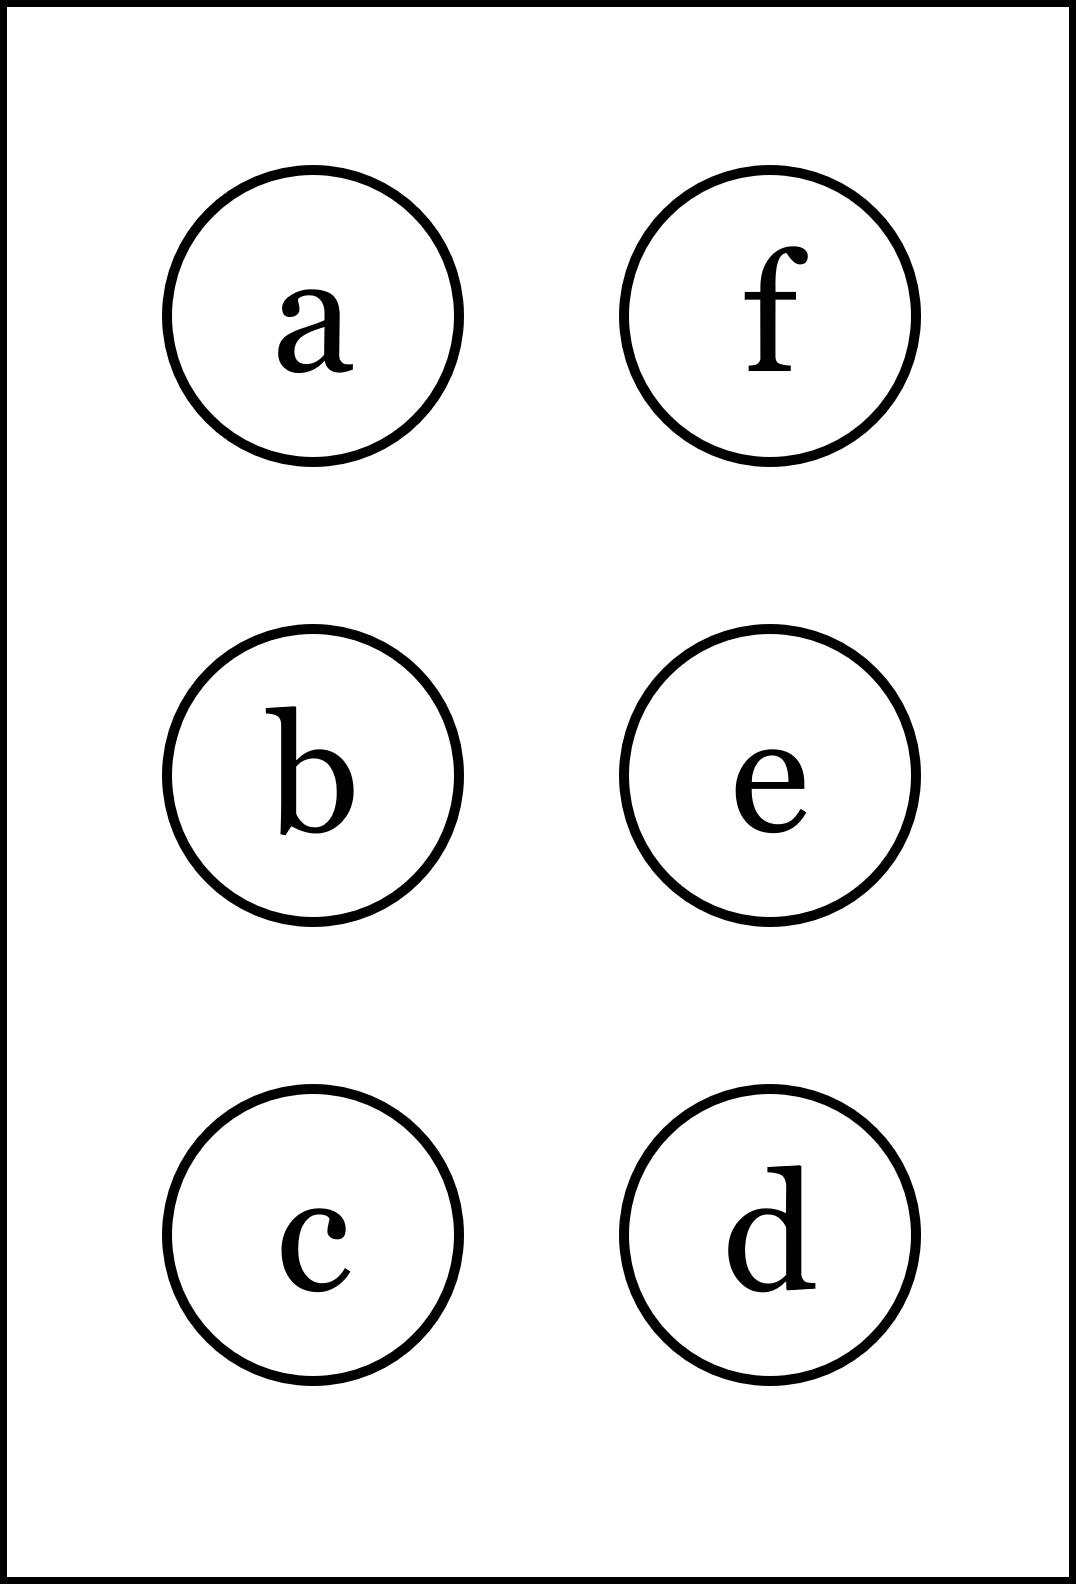
\includegraphics[height=40mm]{../images/braille.png}
{\small Písmeno Braillovej abecedy}
\end{center}
\end{minipage}
\end{center}
\end{minipage}
&
\begin{minipage}[c][104.5mm][t]{0.5\linewidth}
\begin{center}
\vspace{7mm}
{\huge Stacionární body, skupina \textit{Lambda $\lambda$} -\romannumeral4}\\[5mm]
\textit{Jméno:}\phantom{xxxxxxxxxxxxxxxxxxxxxxxxxxxxxxxxxxxxxxxxxxxxxxxxxxxxxxxxxxxxxxxxx}\\[5mm]
\begin{minipage}{0.95\linewidth}
\begin{center}
{\small V \textbf{(a)} zjisti jestli $f(x)$ \textbf{roste} v bode $x_0$. V \textbf{(b)} zjisti jestli je $f(x)$ v bode $x_0$ \textbf{ryze konvexní}.\\V \textbf{(c)} spočti \textbf{součet} x-ových souřadnic stacionárního a inflexního bodu. V \textbf{(d)} najdi x-ovou souřadnici stacionárního bodu a rozhodli jestli to je \textbf{lomax, lomin či inflex}.\\Pokud se výsledky shodujú s těmi za otazníky, tak napravo obarvi příslušející kroužek načerno.\\\textbf{Spolu odevzdejte výsledné slovo}}.
\end{center}
\end{minipage}
\\[1mm]
\begin{minipage}{0.79\linewidth}
\begin{center}
\begin{varwidth}{\linewidth}
\begin{enumerate}
\normalsize
\item $f(x)=\cfrac{5x^2-2x+7}{-3x+3}\enspace , \enspace x_0=-2$\quad \dotfill\; ???\;\dotfill \quad \text{ne}
\item $f(x)=2x^4-3x^3-4x^2+x+1\enspace , \enspace x_0=-2$\quad \dotfill\; ???\;\dotfill \quad \text{ne}
\item $f(x)=6xe^{3x}$\quad \dotfill\; ???\;\dotfill \quad $\nicefrac{1}{3}$
\item $f(x)=\sqrt{4x^2-2x+1}$\quad \dotfill\; ???\;\dotfill \quad $\nicefrac{1}{4}\enspace , \enspace\mathrm{lomax}$
\item \quad \dotfill\; ???\;\dotfill \quad nebarvi
\item \quad \dotfill\; ???\;\dotfill \quad nebarvi
\end{enumerate}
\end{varwidth}
\end{center}
\end{minipage}
\begin{minipage}{0.20\linewidth}
\begin{center}
{\Huge\bfseries 4.} \\[2mm]
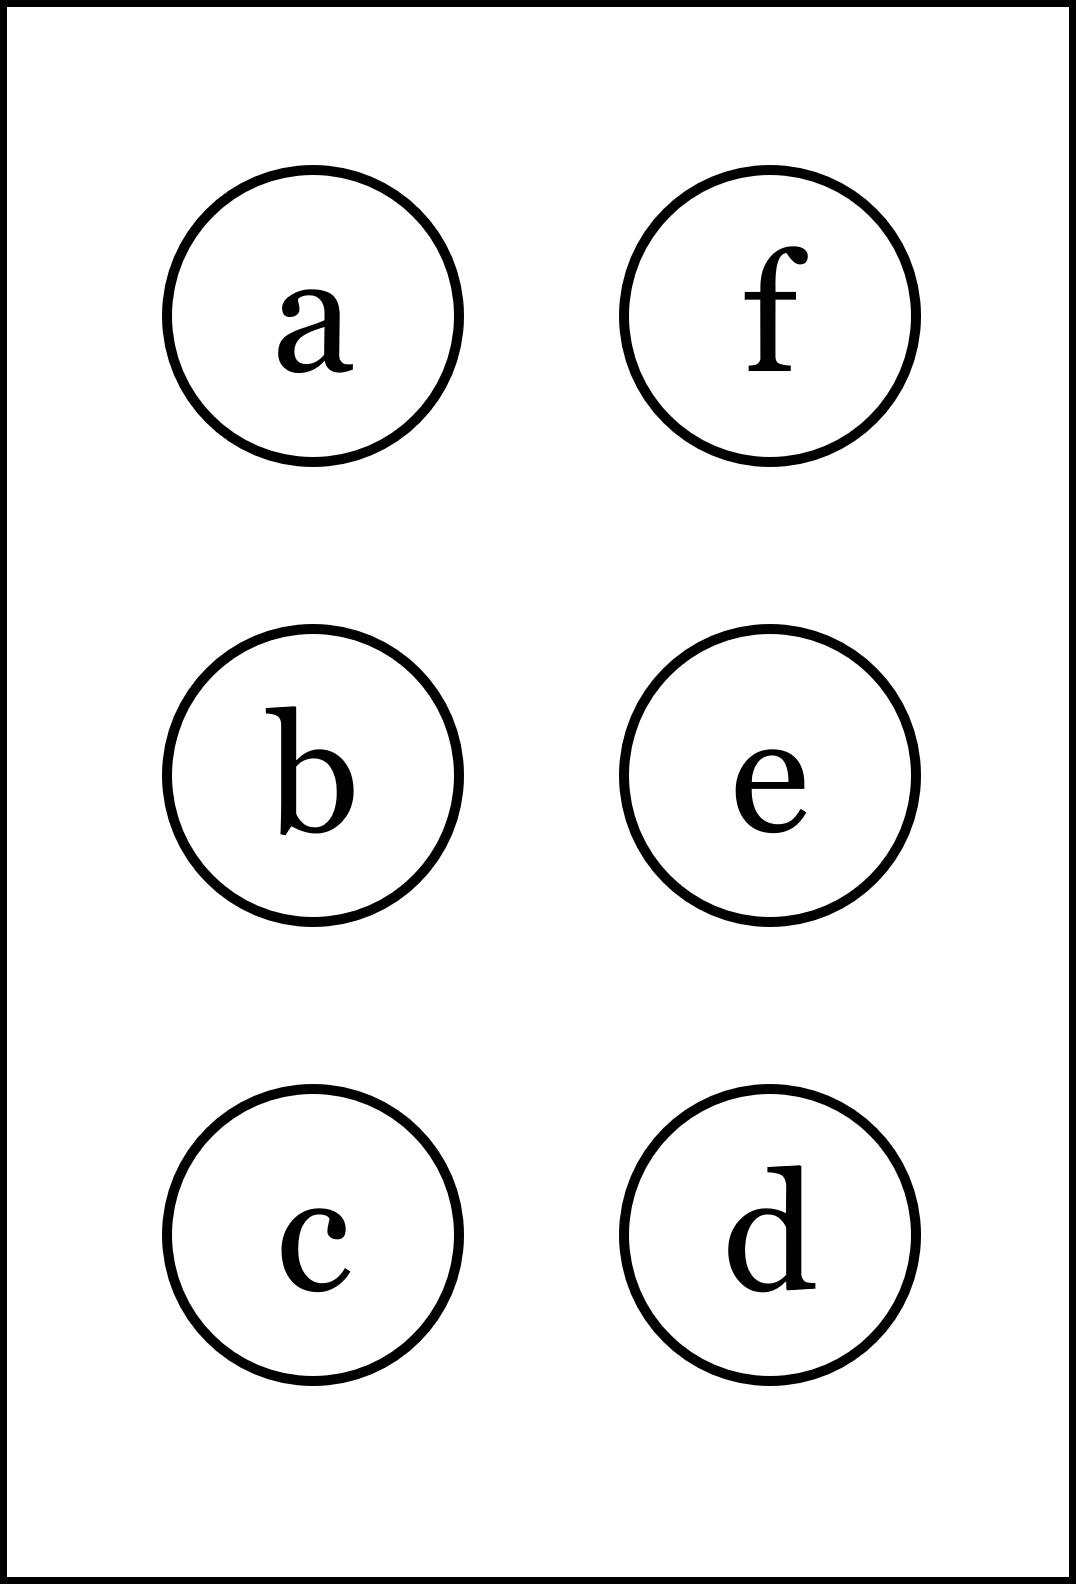
\includegraphics[height=40mm]{../images/braille.png}
{\small Písmeno Braillovej abecedy}
\end{center}
\end{minipage}
\end{center}
\end{minipage}
%
\end{tabular}
\newpage
\thispagestyle{empty}
\begin{tabular}{c:c}
\begin{minipage}[c][104.5mm][t]{0.5\linewidth}
\begin{center}
\vspace{7mm}
{\huge Stacionární body, skupina \textit{Mu $\mu$} -\romannumeral1}\\[5mm]
\textit{Jméno:}\phantom{xxxxxxxxxxxxxxxxxxxxxxxxxxxxxxxxxxxxxxxxxxxxxxxxxxxxxxxxxxxxxxxxx}\\[5mm]
\begin{minipage}{0.95\linewidth}
\begin{center}
{\small V \textbf{(a)} zjisti jestli $f(x)$ \textbf{roste} v bode $x_0$. V \textbf{(b)} zjisti jestli je $f(x)$ v bode $x_0$ \textbf{ryze konvexní}.\\V \textbf{(c)} spočti \textbf{součet} x-ových souřadnic stacionárního a inflexního bodu. V \textbf{(d)} najdi x-ovou souřadnici stacionárního bodu a rozhodli jestli to je \textbf{lomax, lomin či inflex}.\\Pokud se výsledky shodujú s těmi za otazníky, tak napravo obarvi příslušející kroužek načerno.\\\textbf{Spolu odevzdejte výsledné slovo}}.
\end{center}
\end{minipage}
\\[1mm]
\begin{minipage}{0.79\linewidth}
\begin{center}
\begin{varwidth}{\linewidth}
\begin{enumerate}
\normalsize
\item $f(x)=\cfrac{-3x^2-7x-4}{4x+2}\enspace , \enspace x_0=1$\quad \dotfill\; ???\;\dotfill \quad \text{ano}
\item $f(x)=-3x^4+5x^3+4x^2-2x+3\enspace , \enspace x_0=-2$\quad \dotfill\; ???\;\dotfill \quad \text{ne}
\item $f(x)=-8xe^{-x}$\quad \dotfill\; ???\;\dotfill \quad $3$
\item $f(x)=\sqrt{2x^2+3x+2}$\quad \dotfill\; ???\;\dotfill \quad $\nicefrac{-3}{4}\enspace , \enspace \mathrm{lomin}$
\item \quad \dotfill\; ???\;\dotfill \quad nebarvi
\item \quad \dotfill\; ???\;\dotfill \quad vybarvi
\end{enumerate}
\end{varwidth}
\end{center}
\end{minipage}
\begin{minipage}{0.20\linewidth}
\begin{center}
{\Huge\bfseries 1.} \\[2mm]
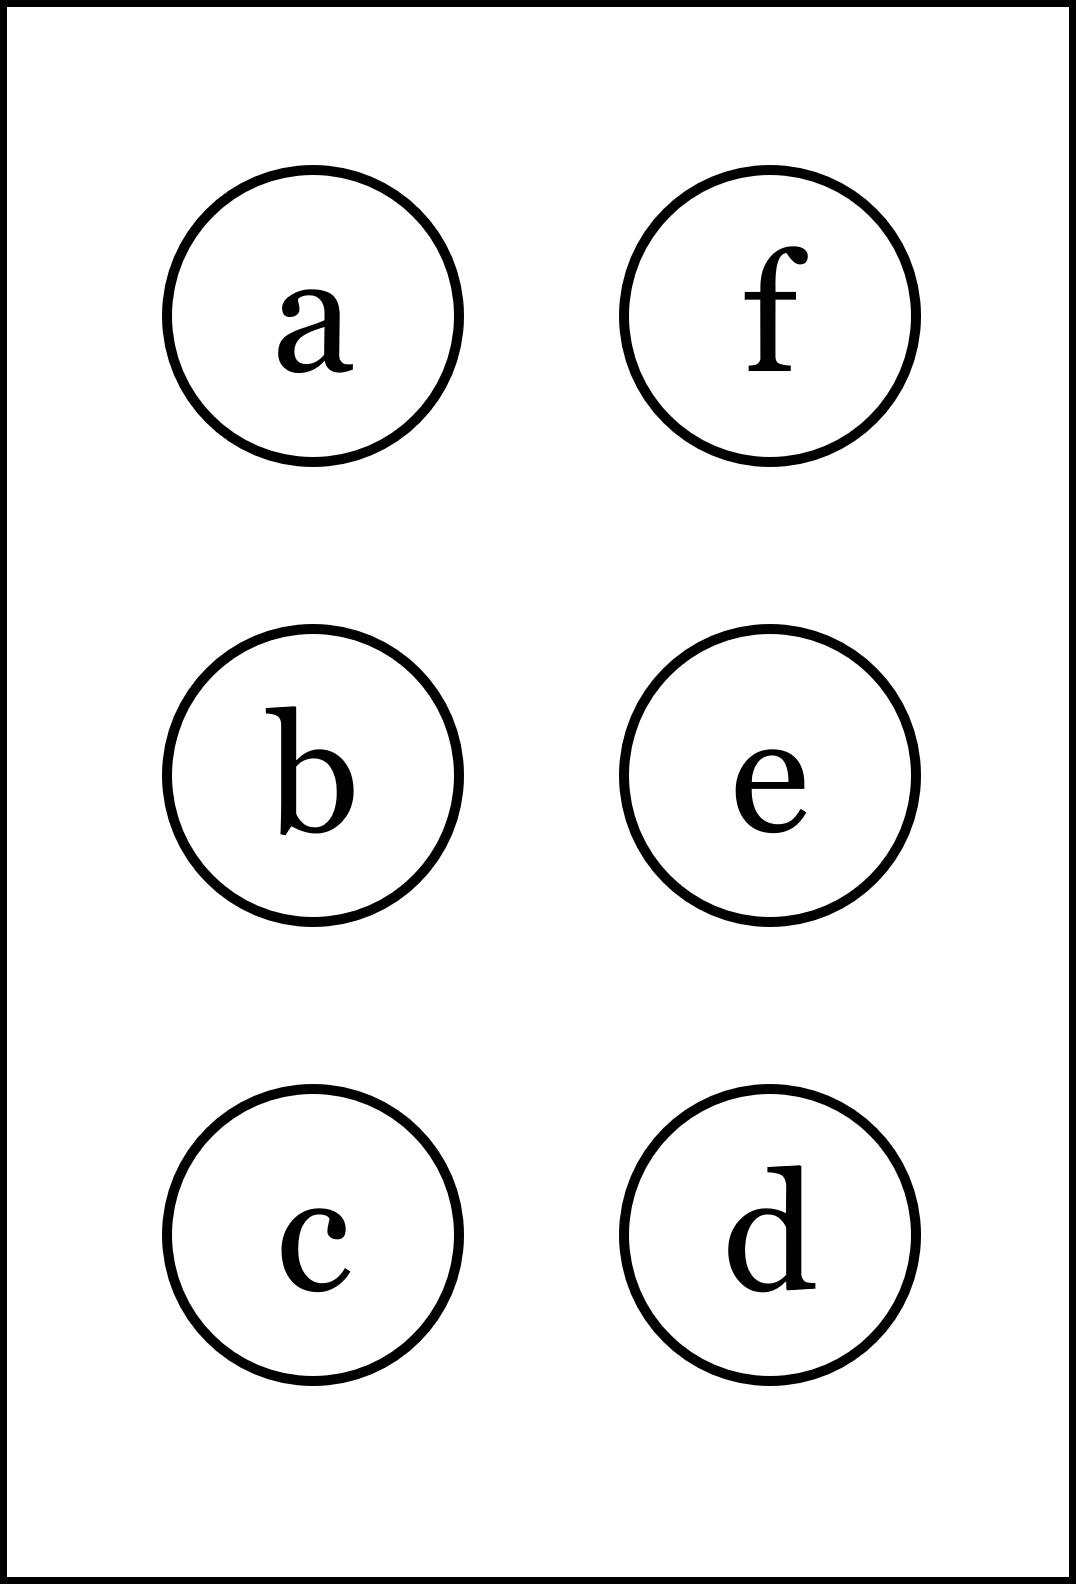
\includegraphics[height=40mm]{../images/braille.png}
{\small Písmeno Braillovej abecedy}
\end{center}
\end{minipage}
\end{center}
\end{minipage}
&
\begin{minipage}[c][104.5mm][t]{0.5\linewidth}
\begin{center}
\vspace{7mm}
{\huge Stacionární body, skupina \textit{Mu $\mu$} -\romannumeral2}\\[5mm]
\textit{Jméno:}\phantom{xxxxxxxxxxxxxxxxxxxxxxxxxxxxxxxxxxxxxxxxxxxxxxxxxxxxxxxxxxxxxxxxx}\\[5mm]
\begin{minipage}{0.95\linewidth}
\begin{center}
{\small V \textbf{(a)} zjisti jestli $f(x)$ \textbf{roste} v bode $x_0$. V \textbf{(b)} zjisti jestli je $f(x)$ v bode $x_0$ \textbf{ryze konvexní}.\\V \textbf{(c)} spočti \textbf{součet} x-ových souřadnic stacionárního a inflexního bodu. V \textbf{(d)} najdi x-ovou souřadnici stacionárního bodu a rozhodli jestli to je \textbf{lomax, lomin či inflex}.\\Pokud se výsledky shodujú s těmi za otazníky, tak napravo obarvi příslušející kroužek načerno.\\\textbf{Spolu odevzdejte výsledné slovo}}.
\end{center}
\end{minipage}
\\[1mm]
\begin{minipage}{0.79\linewidth}
\begin{center}
\begin{varwidth}{\linewidth}
\begin{enumerate}
\normalsize
\item $f(x)=\cfrac{9x^2+x-3}{5x+6}\enspace , \enspace x_0=-1$\quad \dotfill\; ???\;\dotfill \quad \text{ano}
\item $f(x)=x^4+2x^3-3x^2+5x-5\enspace , \enspace x_0=4$\quad \dotfill\; ???\;\dotfill \quad \text{ano}
\item $f(x)=xe^{-x}$\quad \dotfill\; ???\;\dotfill \quad $-1$
\item $f(x)=\sqrt{3x^2-2x+2}$\quad \dotfill\; ???\;\dotfill \quad $\nicefrac{1}{3}\enspace , \enspace\mathrm{lomax}$
\item \quad \dotfill\; ???\;\dotfill \quad nebarvi
\item \quad \dotfill\; ???\;\dotfill \quad vybarvi
\end{enumerate}
\end{varwidth}
\end{center}
\end{minipage}
\begin{minipage}{0.20\linewidth}
\begin{center}
{\Huge\bfseries 2.} \\[2mm]
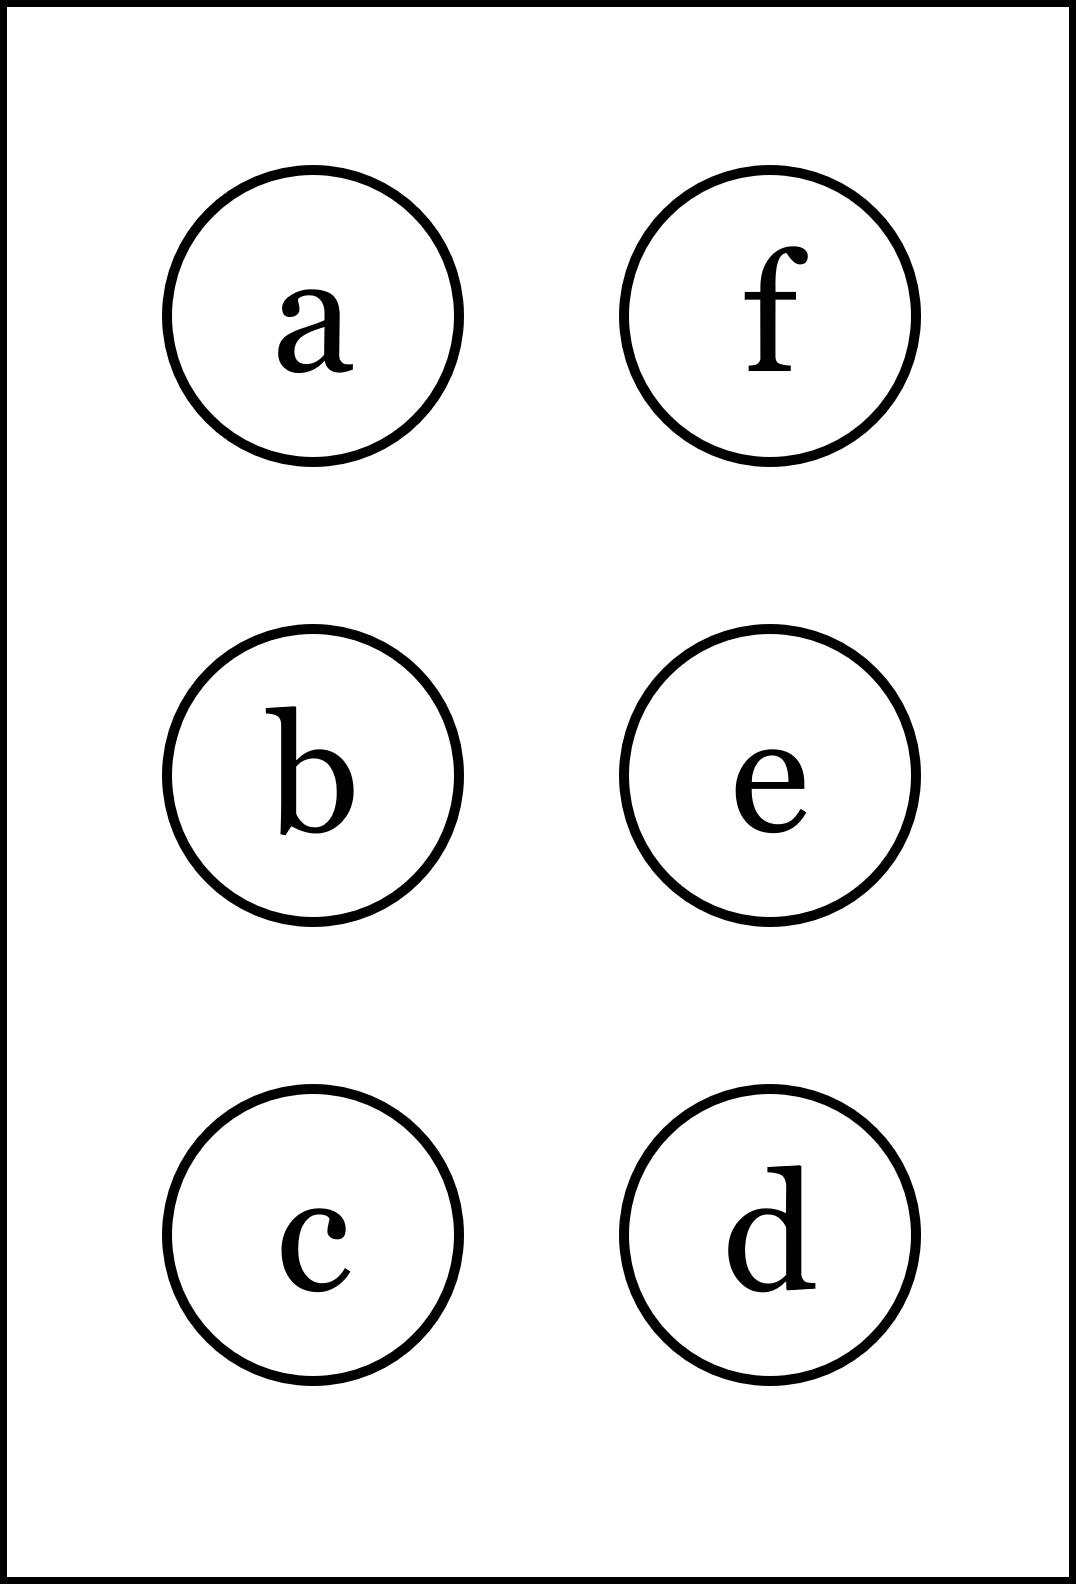
\includegraphics[height=40mm]{../images/braille.png}
{\small Písmeno Braillovej abecedy}
\end{center}
\end{minipage}
\end{center}
\end{minipage}
\\ \hdashline
\begin{minipage}[c][104.5mm][t]{0.5\linewidth}
\begin{center}
\vspace{7mm}
{\huge Stacionární body, skupina \textit{Mu $\mu$} -\romannumeral3}\\[5mm]
\textit{Jméno:}\phantom{xxxxxxxxxxxxxxxxxxxxxxxxxxxxxxxxxxxxxxxxxxxxxxxxxxxxxxxxxxxxxxxxx}\\[5mm]
\begin{minipage}{0.95\linewidth}
\begin{center}
{\small V \textbf{(a)} zjisti jestli $f(x)$ \textbf{roste} v bode $x_0$. V \textbf{(b)} zjisti jestli je $f(x)$ v bode $x_0$ \textbf{ryze konvexní}.\\V \textbf{(c)} spočti \textbf{součet} x-ových souřadnic stacionárního a inflexního bodu. V \textbf{(d)} najdi x-ovou souřadnici stacionárního bodu a rozhodli jestli to je \textbf{lomax, lomin či inflex}.\\Pokud se výsledky shodujú s těmi za otazníky, tak napravo obarvi příslušející kroužek načerno.\\\textbf{Spolu odevzdejte výsledné slovo}}.
\end{center}
\end{minipage}
\\[1mm]
\begin{minipage}{0.79\linewidth}
\begin{center}
\begin{varwidth}{\linewidth}
\begin{enumerate}
\normalsize
\item $f(x)=\cfrac{x^2-5x-5}{-2x-5}\enspace , \enspace x_0=-2$\quad \dotfill\; ???\;\dotfill \quad \text{ne}
\item $f(x)=4x^4+2x^3+8x^2-2x+3\enspace , \enspace x_0=1$\quad \dotfill\; ???\;\dotfill \quad \text{ano}
\item $f(x)=8xe^{4x}$\quad \dotfill\; ???\;\dotfill \quad $\nicefrac{-3}{4}$
\item $f(x)=\sqrt{x^2-2x+2}$\quad \dotfill\; ???\;\dotfill \quad $1\enspace , \enspace\mathrm{inflex}$
\item \quad \dotfill\; ???\;\dotfill \quad vybarvi
\item \quad \dotfill\; ???\;\dotfill \quad vybarvi
\end{enumerate}
\end{varwidth}
\end{center}
\end{minipage}
\begin{minipage}{0.20\linewidth}
\begin{center}
{\Huge\bfseries 3.} \\[2mm]
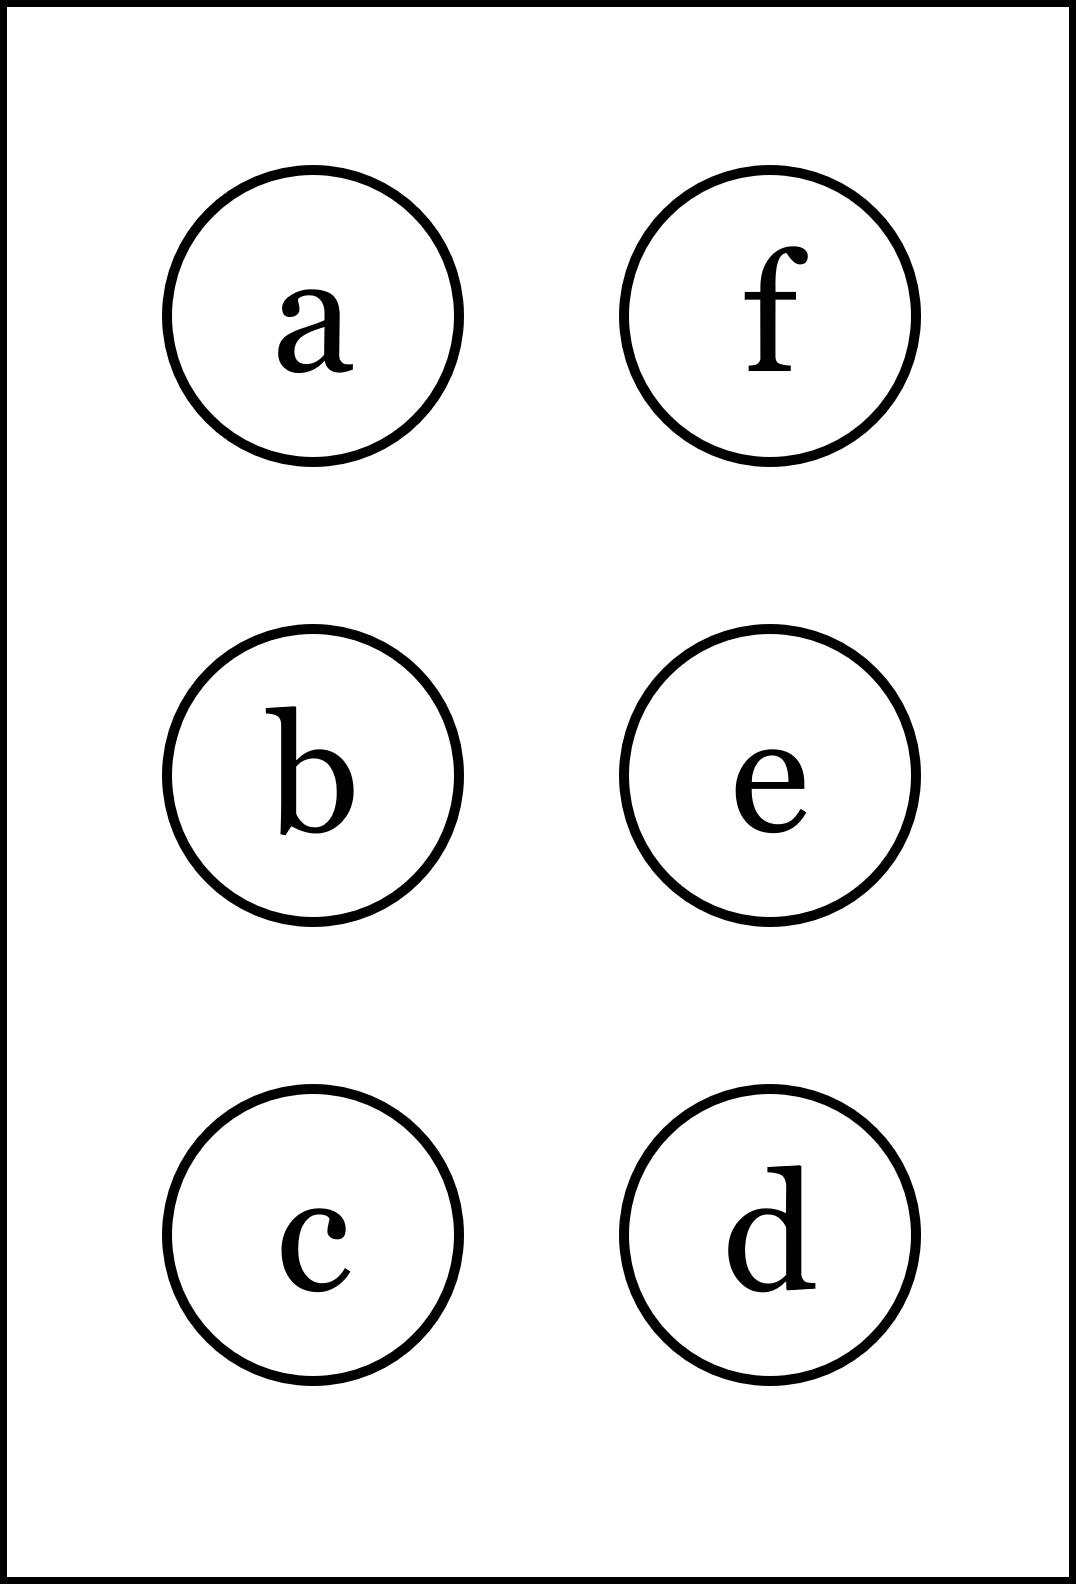
\includegraphics[height=40mm]{../images/braille.png}
{\small Písmeno Braillovej abecedy}
\end{center}
\end{minipage}
\end{center}
\end{minipage}
&
\begin{minipage}[c][104.5mm][t]{0.5\linewidth}
\begin{center}
\vspace{7mm}
{\huge Stacionární body, skupina \textit{Mu $\mu$} -\romannumeral4}\\[5mm]
\textit{Jméno:}\phantom{xxxxxxxxxxxxxxxxxxxxxxxxxxxxxxxxxxxxxxxxxxxxxxxxxxxxxxxxxxxxxxxxx}\\[5mm]
\begin{minipage}{0.95\linewidth}
\begin{center}
{\small V \textbf{(a)} zjisti jestli $f(x)$ \textbf{roste} v bode $x_0$. V \textbf{(b)} zjisti jestli je $f(x)$ v bode $x_0$ \textbf{ryze konvexní}.\\V \textbf{(c)} spočti \textbf{součet} x-ových souřadnic stacionárního a inflexního bodu. V \textbf{(d)} najdi x-ovou souřadnici stacionárního bodu a rozhodli jestli to je \textbf{lomax, lomin či inflex}.\\Pokud se výsledky shodujú s těmi za otazníky, tak napravo obarvi příslušející kroužek načerno.\\\textbf{Spolu odevzdejte výsledné slovo}}.
\end{center}
\end{minipage}
\\[1mm]
\begin{minipage}{0.79\linewidth}
\begin{center}
\begin{varwidth}{\linewidth}
\begin{enumerate}
\normalsize
\item $f(x)=\cfrac{3x^2-6x-5}{3x-4}\enspace , \enspace x_0=3$\quad \dotfill\; ???\;\dotfill \quad \text{ano}
\item $f(x)=x^4+7x^3+3x^2-4x-6\enspace , \enspace x_0=-2$\quad \dotfill\; ???\;\dotfill \quad \text{ano}
\item $f(x)=-6xe^{x}$\quad \dotfill\; ???\;\dotfill \quad $-3$
\item $f(x)=\sqrt{3x^2-3x+2}$\quad \dotfill\; ???\;\dotfill \quad $\nicefrac{1}{2}\enspace , \enspace\mathrm{lomax}$
\item \quad \dotfill\; ???\;\dotfill \quad vybarvi
\item \quad \dotfill\; ???\;\dotfill \quad nebarvi
\end{enumerate}
\end{varwidth}
\end{center}
\end{minipage}
\begin{minipage}{0.20\linewidth}
\begin{center}
{\Huge\bfseries 4.} \\[2mm]
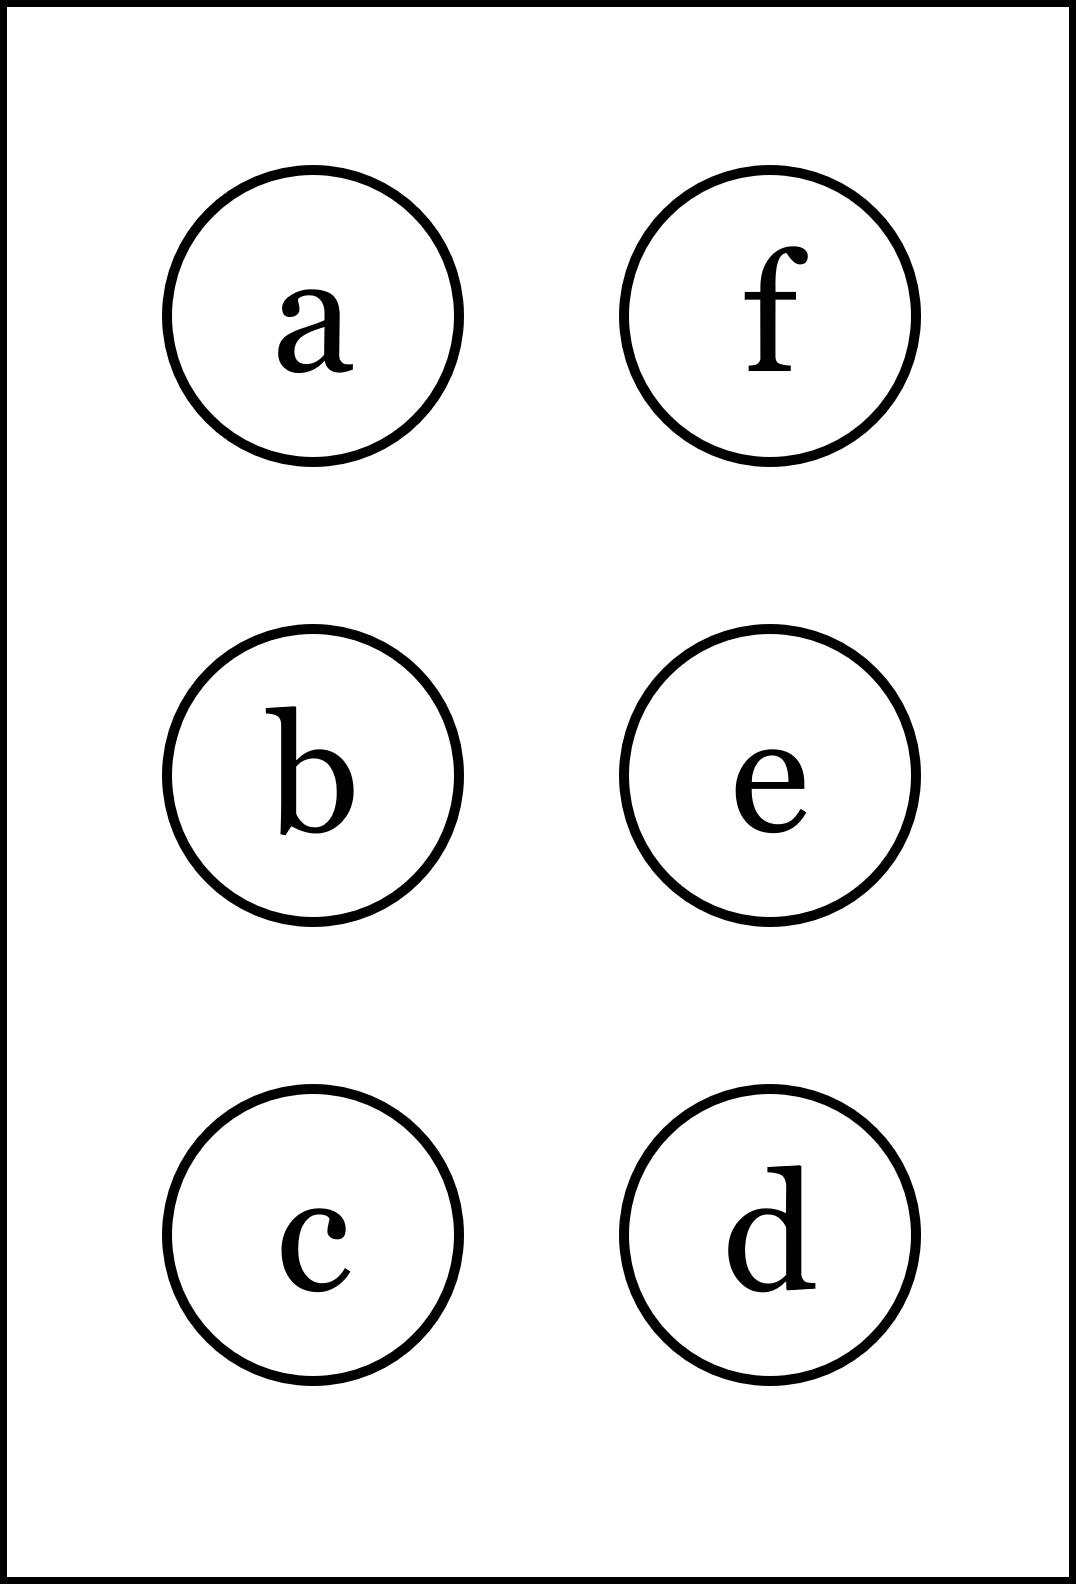
\includegraphics[height=40mm]{../images/braille.png}
{\small Písmeno Braillovej abecedy}
\end{center}
\end{minipage}
\end{center}
\end{minipage}
%
\end{tabular}
\newpage
\thispagestyle{empty}
\begin{tabular}{c:c}
\begin{minipage}[c][104.5mm][t]{0.5\linewidth}
\begin{center}
\vspace{7mm}
{\huge Stacionární body, skupina \textit{Nu $\nu$} -\romannumeral1}\\[5mm]
\textit{Jméno:}\phantom{xxxxxxxxxxxxxxxxxxxxxxxxxxxxxxxxxxxxxxxxxxxxxxxxxxxxxxxxxxxxxxxxx}\\[5mm]
\begin{minipage}{0.95\linewidth}
\begin{center}
{\small V \textbf{(a)} zjisti jestli $f(x)$ \textbf{roste} v bode $x_0$. V \textbf{(b)} zjisti jestli je $f(x)$ v bode $x_0$ \textbf{ryze konvexní}.\\V \textbf{(c)} spočti \textbf{součet} x-ových souřadnic stacionárního a inflexního bodu. V \textbf{(d)} najdi x-ovou souřadnici stacionárního bodu a rozhodli jestli to je \textbf{lomax, lomin či inflex}.\\Pokud se výsledky shodujú s těmi za otazníky, tak napravo obarvi příslušející kroužek načerno.\\\textbf{Spolu odevzdejte výsledné slovo}}.
\end{center}
\end{minipage}
\\[1mm]
\begin{minipage}{0.79\linewidth}
\begin{center}
\begin{varwidth}{\linewidth}
\begin{enumerate}
\normalsize
\item $f(x)=\cfrac{-2x^2+2x+7}{7x-1}\enspace , \enspace x_0=1$\quad \dotfill\; ???\;\dotfill \quad \text{ne}
\item $f(x)=5x^4+4x^3-8x^2-4x-2\enspace , \enspace x_0=-1$\quad \dotfill\; ???\;\dotfill \quad \text{ano}
\item $f(x)=-2xe^{4x}$\quad \dotfill\; ???\;\dotfill \quad $\nicefrac{-3}{4}$
\item $f(x)=\sqrt{4x^2+3x+3}$\quad \dotfill\; ???\;\dotfill \quad $\nicefrac{-3}{8}\enspace , \enspace\mathrm{lomax}$
\item \quad \dotfill\; ???\;\dotfill \quad vybarvi
\item \quad \dotfill\; ???\;\dotfill \quad nebarvi
\end{enumerate}
\end{varwidth}
\end{center}
\end{minipage}
\begin{minipage}{0.20\linewidth}
\begin{center}
{\Huge\bfseries 1.} \\[2mm]
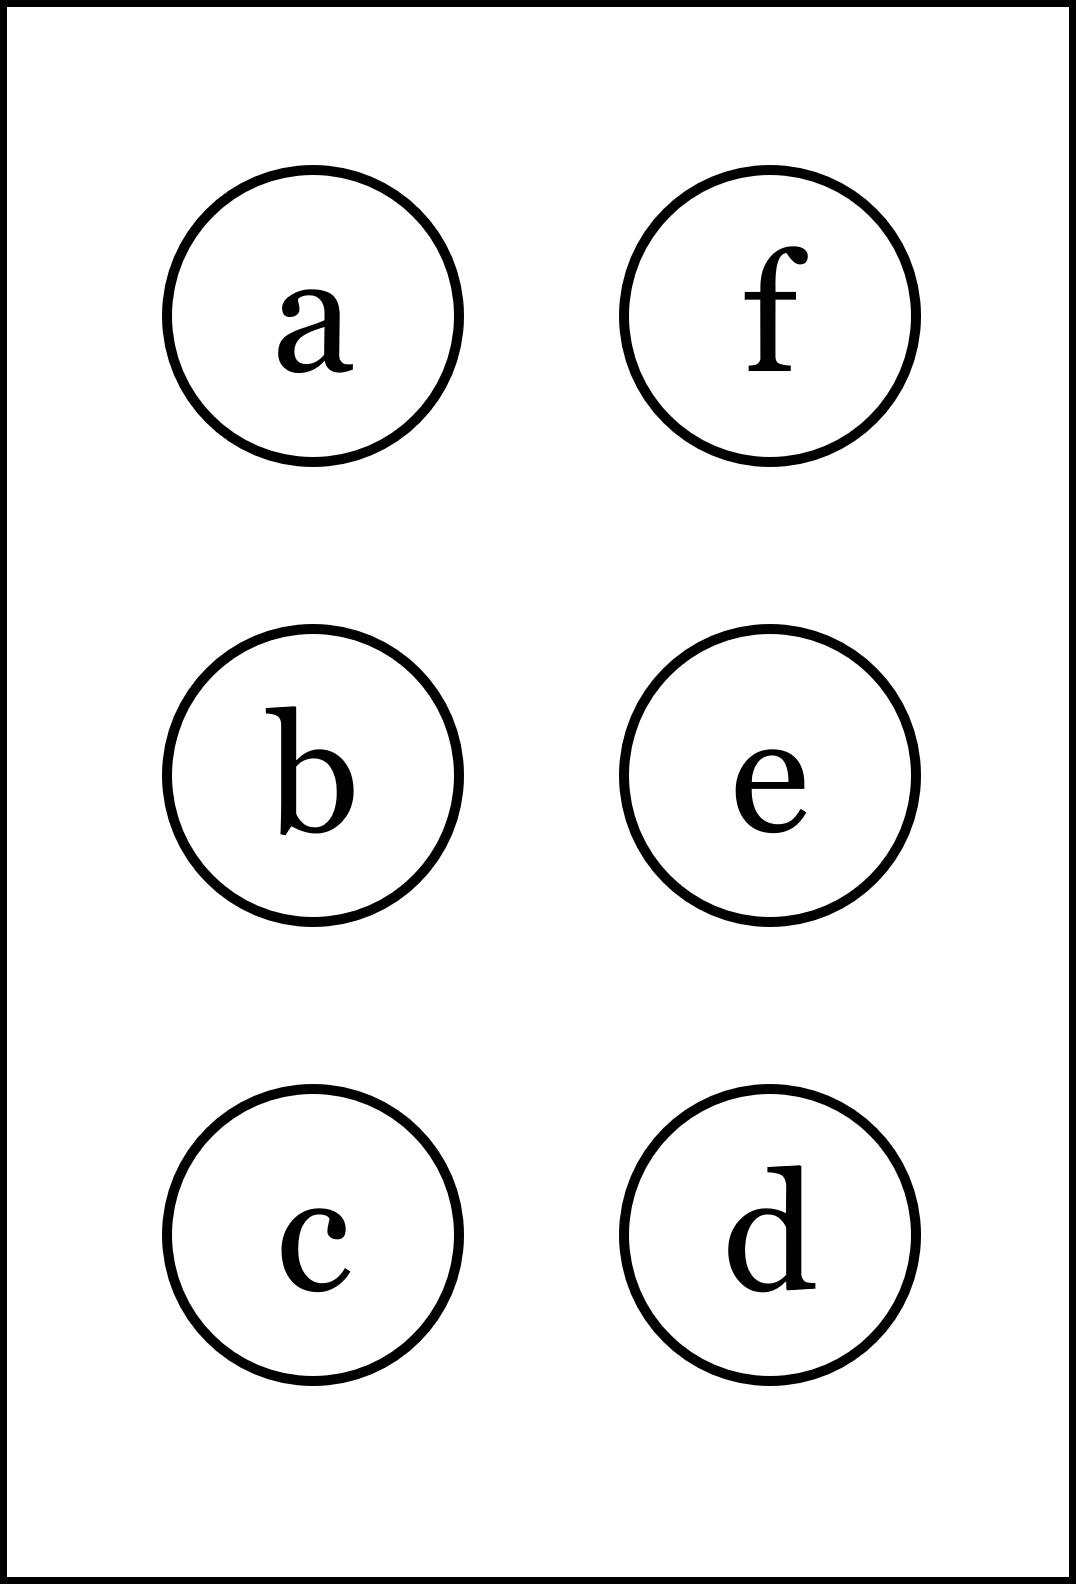
\includegraphics[height=40mm]{../images/braille.png}
{\small Písmeno Braillovej abecedy}
\end{center}
\end{minipage}
\end{center}
\end{minipage}
&
\begin{minipage}[c][104.5mm][t]{0.5\linewidth}
\begin{center}
\vspace{7mm}
{\huge Stacionární body, skupina \textit{Nu $\nu$} -\romannumeral2}\\[5mm]
\textit{Jméno:}\phantom{xxxxxxxxxxxxxxxxxxxxxxxxxxxxxxxxxxxxxxxxxxxxxxxxxxxxxxxxxxxxxxxxx}\\[5mm]
\begin{minipage}{0.95\linewidth}
\begin{center}
{\small V \textbf{(a)} zjisti jestli $f(x)$ \textbf{roste} v bode $x_0$. V \textbf{(b)} zjisti jestli je $f(x)$ v bode $x_0$ \textbf{ryze konvexní}.\\V \textbf{(c)} spočti \textbf{součet} x-ových souřadnic stacionárního a inflexního bodu. V \textbf{(d)} najdi x-ovou souřadnici stacionárního bodu a rozhodli jestli to je \textbf{lomax, lomin či inflex}.\\Pokud se výsledky shodujú s těmi za otazníky, tak napravo obarvi příslušející kroužek načerno.\\\textbf{Spolu odevzdejte výsledné slovo}}.
\end{center}
\end{minipage}
\\[1mm]
\begin{minipage}{0.79\linewidth}
\begin{center}
\begin{varwidth}{\linewidth}
\begin{enumerate}
\normalsize
\item $f(x)=\cfrac{x^2-8x+8}{x-2}\enspace , \enspace x_0=1$\quad \dotfill\; ???\;\dotfill \quad \text{ano}
\item $f(x)=-x^4+8x^3+x^2-x+6\enspace , \enspace x_0=2$\quad \dotfill\; ???\;\dotfill \quad \text{ne}
\item $f(x)=8xe^{x}$\quad \dotfill\; ???\;\dotfill \quad $-3$
\item $f(x)=\sqrt{2x^2-2x+2}$\quad \dotfill\; ???\;\dotfill \quad $\nicefrac{1}{2}\enspace , \enspace \mathrm{lomin}$
\item \quad \dotfill\; ???\;\dotfill \quad nebarvi
\item \quad \dotfill\; ???\;\dotfill \quad nebarvi
\end{enumerate}
\end{varwidth}
\end{center}
\end{minipage}
\begin{minipage}{0.20\linewidth}
\begin{center}
{\Huge\bfseries 2.} \\[2mm]
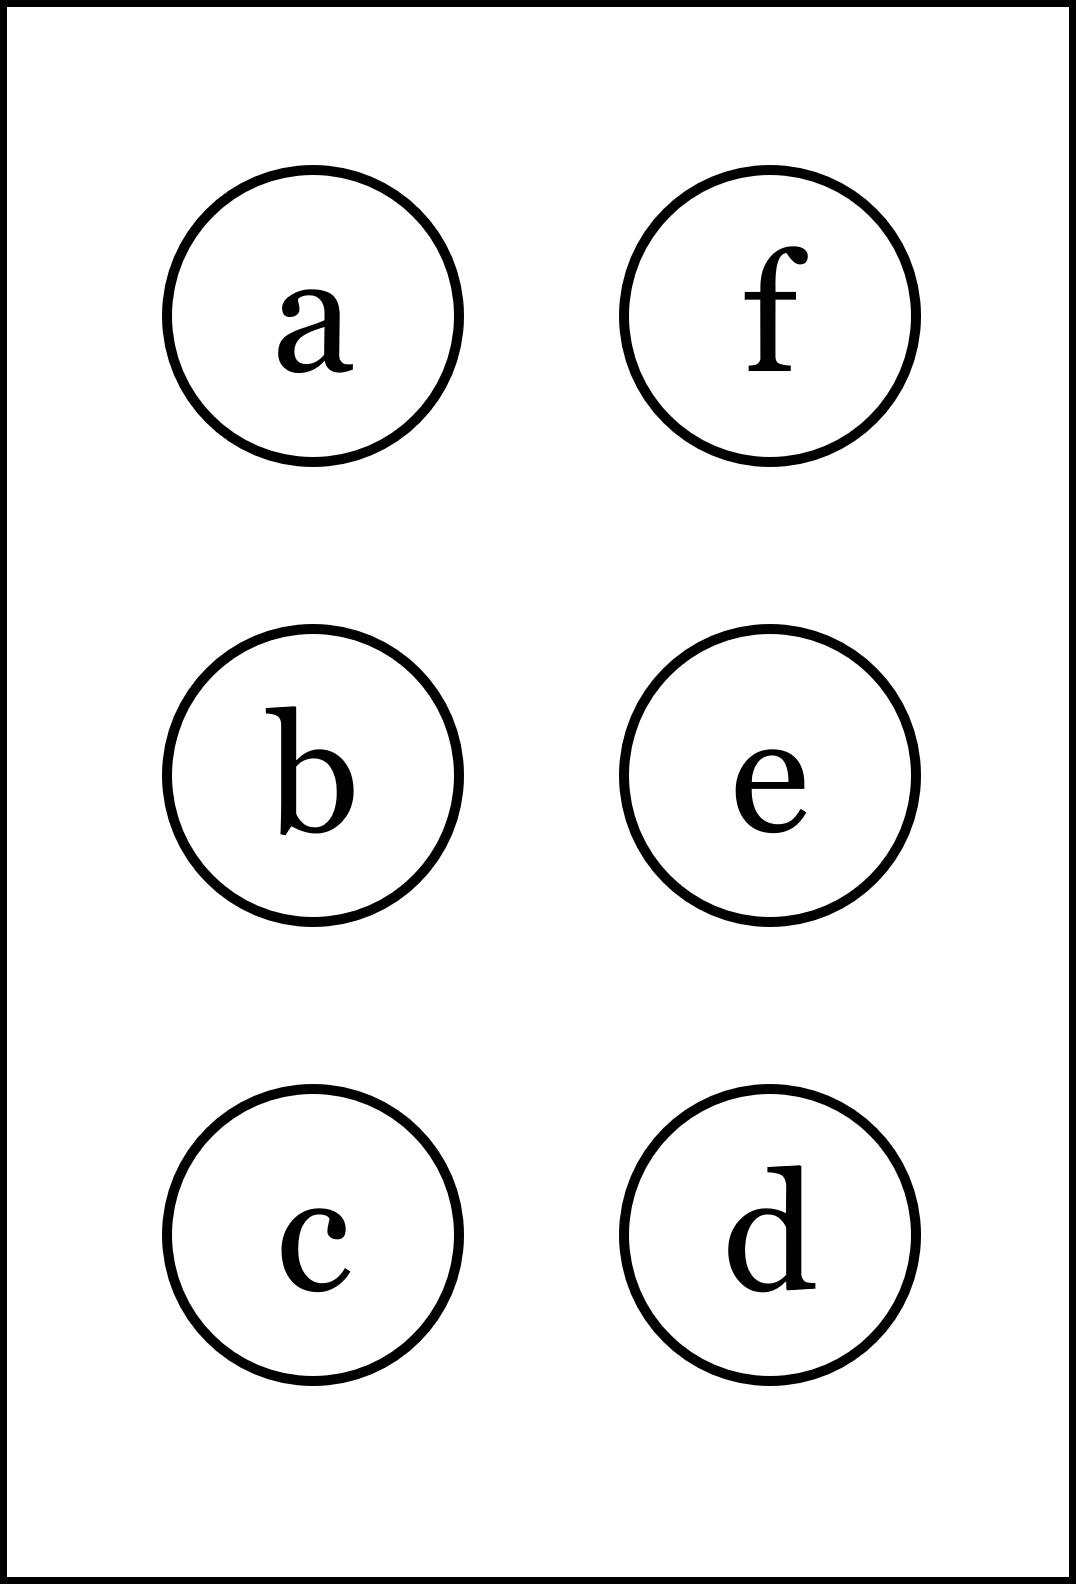
\includegraphics[height=40mm]{../images/braille.png}
{\small Písmeno Braillovej abecedy}
\end{center}
\end{minipage}
\end{center}
\end{minipage}
\\ \hdashline
\begin{minipage}[c][104.5mm][t]{0.5\linewidth}
\begin{center}
\vspace{7mm}
{\huge Stacionární body, skupina \textit{Nu $\nu$} -\romannumeral3}\\[5mm]
\textit{Jméno:}\phantom{xxxxxxxxxxxxxxxxxxxxxxxxxxxxxxxxxxxxxxxxxxxxxxxxxxxxxxxxxxxxxxxxx}\\[5mm]
\begin{minipage}{0.95\linewidth}
\begin{center}
{\small V \textbf{(a)} zjisti jestli $f(x)$ \textbf{roste} v bode $x_0$. V \textbf{(b)} zjisti jestli je $f(x)$ v bode $x_0$ \textbf{ryze konvexní}.\\V \textbf{(c)} spočti \textbf{součet} x-ových souřadnic stacionárního a inflexního bodu. V \textbf{(d)} najdi x-ovou souřadnici stacionárního bodu a rozhodli jestli to je \textbf{lomax, lomin či inflex}.\\Pokud se výsledky shodujú s těmi za otazníky, tak napravo obarvi příslušející kroužek načerno.\\\textbf{Spolu odevzdejte výsledné slovo}}.
\end{center}
\end{minipage}
\\[1mm]
\begin{minipage}{0.79\linewidth}
\begin{center}
\begin{varwidth}{\linewidth}
\begin{enumerate}
\normalsize
\item $f(x)=\cfrac{-7x^2-7x+8}{-2x-6}\enspace , \enspace x_0=2$\quad \dotfill\; ???\;\dotfill \quad \text{ano}
\item $f(x)=7x^4+5x^3-2x^2-x+3\enspace , \enspace x_0=-1$\quad \dotfill\; ???\;\dotfill \quad \text{ne}
\item $f(x)=-3xe^{4x}$\quad \dotfill\; ???\;\dotfill \quad $\nicefrac{-3}{4}$
\item $f(x)=\sqrt{3x^2-2x+2}$\quad \dotfill\; ???\;\dotfill \quad $\nicefrac{1}{3}\enspace , \enspace\mathrm{lomax}$
\item \quad \dotfill\; ???\;\dotfill \quad nebarvi
\item \quad \dotfill\; ???\;\dotfill \quad nebarvi
\end{enumerate}
\end{varwidth}
\end{center}
\end{minipage}
\begin{minipage}{0.20\linewidth}
\begin{center}
{\Huge\bfseries 3.} \\[2mm]
\includegraphics[height=40mm]{../images/braille.png}
{\small Písmeno Braillovej abecedy}
\end{center}
\end{minipage}
\end{center}
\end{minipage}
&
\begin{minipage}[c][104.5mm][t]{0.5\linewidth}
\begin{center}
\vspace{7mm}
{\huge Stacionární body, skupina \textit{Nu $\nu$} -\romannumeral4}\\[5mm]
\textit{Jméno:}\phantom{xxxxxxxxxxxxxxxxxxxxxxxxxxxxxxxxxxxxxxxxxxxxxxxxxxxxxxxxxxxxxxxxx}\\[5mm]
\begin{minipage}{0.95\linewidth}
\begin{center}
{\small V \textbf{(a)} zjisti jestli $f(x)$ \textbf{roste} v bode $x_0$. V \textbf{(b)} zjisti jestli je $f(x)$ v bode $x_0$ \textbf{ryze konvexní}.\\V \textbf{(c)} spočti \textbf{součet} x-ových souřadnic stacionárního a inflexního bodu. V \textbf{(d)} najdi x-ovou souřadnici stacionárního bodu a rozhodli jestli to je \textbf{lomax, lomin či inflex}.\\Pokud se výsledky shodujú s těmi za otazníky, tak napravo obarvi příslušející kroužek načerno.\\\textbf{Spolu odevzdejte výsledné slovo}}.
\end{center}
\end{minipage}
\\[1mm]
\begin{minipage}{0.79\linewidth}
\begin{center}
\begin{varwidth}{\linewidth}
\begin{enumerate}
\normalsize
\item $f(x)=\cfrac{-x^2-5x+7}{2x-7}\enspace , \enspace x_0=-4$\quad \dotfill\; ???\;\dotfill \quad \text{ne}
\item $f(x)=6x^4-4x^3-5x^2-6x-3\enspace , \enspace x_0=-2$\quad \dotfill\; ???\;\dotfill \quad \text{ne}
\item $f(x)=-xe^{2x}$\quad \dotfill\; ???\;\dotfill \quad $\nicefrac{1}{2}$
\item $f(x)=\sqrt{4x^2-4x+4}$\quad \dotfill\; ???\;\dotfill \quad $\nicefrac{1}{2}\enspace , \enspace\mathrm{lomax}$
\item \quad \dotfill\; ???\;\dotfill \quad nebarvi
\item \quad \dotfill\; ???\;\dotfill \quad nebarvi
\end{enumerate}
\end{varwidth}
\end{center}
\end{minipage}
\begin{minipage}{0.20\linewidth}
\begin{center}
{\Huge\bfseries 4.} \\[2mm]
\includegraphics[height=40mm]{../images/braille.png}
{\small Písmeno Braillovej abecedy}
\end{center}
\end{minipage}
\end{center}
\end{minipage}
%
\end{tabular}
\newpage
\thispagestyle{empty}
\begin{tabular}{c:c}
\begin{minipage}[c][104.5mm][t]{0.5\linewidth}
\begin{center}
\vspace{7mm}
{\huge Stacionární body, skupina \textit{Xi $\xi$} -\romannumeral1}\\[5mm]
\textit{Jméno:}\phantom{xxxxxxxxxxxxxxxxxxxxxxxxxxxxxxxxxxxxxxxxxxxxxxxxxxxxxxxxxxxxxxxxx}\\[5mm]
\begin{minipage}{0.95\linewidth}
\begin{center}
{\small V \textbf{(a)} zjisti jestli $f(x)$ \textbf{roste} v bode $x_0$. V \textbf{(b)} zjisti jestli je $f(x)$ v bode $x_0$ \textbf{ryze konvexní}.\\V \textbf{(c)} spočti \textbf{součet} x-ových souřadnic stacionárního a inflexního bodu. V \textbf{(d)} najdi x-ovou souřadnici stacionárního bodu a rozhodli jestli to je \textbf{lomax, lomin či inflex}.\\Pokud se výsledky shodujú s těmi za otazníky, tak napravo obarvi příslušející kroužek načerno.\\\textbf{Spolu odevzdejte výsledné slovo}}.
\end{center}
\end{minipage}
\\[1mm]
\begin{minipage}{0.79\linewidth}
\begin{center}
\begin{varwidth}{\linewidth}
\begin{enumerate}
\normalsize
\item $f(x)=\cfrac{x^2+3x+1}{x-5}\enspace , \enspace x_0=3$\quad \dotfill\; ???\;\dotfill \quad \text{ne}
\item $f(x)=3x^4+4x^3+4x^2-7x+2\enspace , \enspace x_0=2$\quad \dotfill\; ???\;\dotfill \quad \text{ne}
\item $f(x)=6xe^{-3x}$\quad \dotfill\; ???\;\dotfill \quad $1$
\item $f(x)=\sqrt{x^2+3x+4}$\quad \dotfill\; ???\;\dotfill \quad $\nicefrac{-3}{2}\enspace , \enspace\mathrm{lomax}$
\item \quad \dotfill\; ???\;\dotfill \quad vybarvi
\item \quad \dotfill\; ???\;\dotfill \quad nebarvi
\end{enumerate}
\end{varwidth}
\end{center}
\end{minipage}
\begin{minipage}{0.20\linewidth}
\begin{center}
{\Huge\bfseries 1.} \\[2mm]
\includegraphics[height=40mm]{../images/braille.png}
{\small Písmeno Braillovej abecedy}
\end{center}
\end{minipage}
\end{center}
\end{minipage}
&
\begin{minipage}[c][104.5mm][t]{0.5\linewidth}
\begin{center}
\vspace{7mm}
{\huge Stacionární body, skupina \textit{Xi $\xi$} -\romannumeral2}\\[5mm]
\textit{Jméno:}\phantom{xxxxxxxxxxxxxxxxxxxxxxxxxxxxxxxxxxxxxxxxxxxxxxxxxxxxxxxxxxxxxxxxx}\\[5mm]
\begin{minipage}{0.95\linewidth}
\begin{center}
{\small V \textbf{(a)} zjisti jestli $f(x)$ \textbf{roste} v bode $x_0$. V \textbf{(b)} zjisti jestli je $f(x)$ v bode $x_0$ \textbf{ryze konvexní}.\\V \textbf{(c)} spočti \textbf{součet} x-ových souřadnic stacionárního a inflexního bodu. V \textbf{(d)} najdi x-ovou souřadnici stacionárního bodu a rozhodli jestli to je \textbf{lomax, lomin či inflex}.\\Pokud se výsledky shodujú s těmi za otazníky, tak napravo obarvi příslušející kroužek načerno.\\\textbf{Spolu odevzdejte výsledné slovo}}.
\end{center}
\end{minipage}
\\[1mm]
\begin{minipage}{0.79\linewidth}
\begin{center}
\begin{varwidth}{\linewidth}
\begin{enumerate}
\normalsize
\item $f(x)=\cfrac{x^2-2x+1}{-x+2}\enspace , \enspace x_0=-5$\quad \dotfill\; ???\;\dotfill \quad \text{ano}
\item $f(x)=3x^4+3x^3+9x^2+3x+2\enspace , \enspace x_0=-2$\quad \dotfill\; ???\;\dotfill \quad \text{ano}
\item $f(x)=-xe^{-3x}$\quad \dotfill\; ???\;\dotfill \quad $1$
\item $f(x)=\sqrt{4x^2-3x+1}$\quad \dotfill\; ???\;\dotfill \quad $\nicefrac{3}{8}\enspace , \enspace\mathrm{lomax}$
\item \quad \dotfill\; ???\;\dotfill \quad nebarvi
\item \quad \dotfill\; ???\;\dotfill \quad vybarvi
\end{enumerate}
\end{varwidth}
\end{center}
\end{minipage}
\begin{minipage}{0.20\linewidth}
\begin{center}
{\Huge\bfseries 2.} \\[2mm]
\includegraphics[height=40mm]{../images/braille.png}
{\small Písmeno Braillovej abecedy}
\end{center}
\end{minipage}
\end{center}
\end{minipage}
\\ \hdashline
\begin{minipage}[c][104.5mm][t]{0.5\linewidth}
\begin{center}
\vspace{7mm}
{\huge Stacionární body, skupina \textit{Xi $\xi$} -\romannumeral3}\\[5mm]
\textit{Jméno:}\phantom{xxxxxxxxxxxxxxxxxxxxxxxxxxxxxxxxxxxxxxxxxxxxxxxxxxxxxxxxxxxxxxxxx}\\[5mm]
\begin{minipage}{0.95\linewidth}
\begin{center}
{\small V \textbf{(a)} zjisti jestli $f(x)$ \textbf{roste} v bode $x_0$. V \textbf{(b)} zjisti jestli je $f(x)$ v bode $x_0$ \textbf{ryze konvexní}.\\V \textbf{(c)} spočti \textbf{součet} x-ových souřadnic stacionárního a inflexního bodu. V \textbf{(d)} najdi x-ovou souřadnici stacionárního bodu a rozhodli jestli to je \textbf{lomax, lomin či inflex}.\\Pokud se výsledky shodujú s těmi za otazníky, tak napravo obarvi příslušející kroužek načerno.\\\textbf{Spolu odevzdejte výsledné slovo}}.
\end{center}
\end{minipage}
\\[1mm]
\begin{minipage}{0.79\linewidth}
\begin{center}
\begin{varwidth}{\linewidth}
\begin{enumerate}
\normalsize
\item $f(x)=\cfrac{3x^2-3x-5}{-5x+6}\enspace , \enspace x_0=2$\quad \dotfill\; ???\;\dotfill \quad \text{ne}
\item $f(x)=2x^4+7x^3-x^2-x-7\enspace , \enspace x_0=1$\quad \dotfill\; ???\;\dotfill \quad \text{ne}
\item $f(x)=-3xe^{-2x}$\quad \dotfill\; ???\;\dotfill \quad $\nicefrac{-1}{2}$
\item $f(x)=\sqrt{4x^2+2x+1}$\quad \dotfill\; ???\;\dotfill \quad $\nicefrac{-1}{4}\enspace , \enspace\mathrm{inflex}$
\item \quad \dotfill\; ???\;\dotfill \quad vybarvi
\item \quad \dotfill\; ???\;\dotfill \quad nebarvi
\end{enumerate}
\end{varwidth}
\end{center}
\end{minipage}
\begin{minipage}{0.20\linewidth}
\begin{center}
{\Huge\bfseries 3.} \\[2mm]
\includegraphics[height=40mm]{../images/braille.png}
{\small Písmeno Braillovej abecedy}
\end{center}
\end{minipage}
\end{center}
\end{minipage}
&
\begin{minipage}[c][104.5mm][t]{0.5\linewidth}
\begin{center}
\vspace{7mm}
{\huge Stacionární body, skupina \textit{Xi $\xi$} -\romannumeral4}\\[5mm]
\textit{Jméno:}\phantom{xxxxxxxxxxxxxxxxxxxxxxxxxxxxxxxxxxxxxxxxxxxxxxxxxxxxxxxxxxxxxxxxx}\\[5mm]
\begin{minipage}{0.95\linewidth}
\begin{center}
{\small V \textbf{(a)} zjisti jestli $f(x)$ \textbf{roste} v bode $x_0$. V \textbf{(b)} zjisti jestli je $f(x)$ v bode $x_0$ \textbf{ryze konvexní}.\\V \textbf{(c)} spočti \textbf{součet} x-ových souřadnic stacionárního a inflexního bodu. V \textbf{(d)} najdi x-ovou souřadnici stacionárního bodu a rozhodli jestli to je \textbf{lomax, lomin či inflex}.\\Pokud se výsledky shodujú s těmi za otazníky, tak napravo obarvi příslušející kroužek načerno.\\\textbf{Spolu odevzdejte výsledné slovo}}.
\end{center}
\end{minipage}
\\[1mm]
\begin{minipage}{0.79\linewidth}
\begin{center}
\begin{varwidth}{\linewidth}
\begin{enumerate}
\normalsize
\item $f(x)=\cfrac{4x^2-2x+9}{8x+6}\enspace , \enspace x_0=1$\quad \dotfill\; ???\;\dotfill \quad \text{ne}
\item $f(x)=-7x^4+x^3-x^2+x+3\enspace , \enspace x_0=-2$\quad \dotfill\; ???\;\dotfill \quad \text{ne}
\item $f(x)=-8xe^{4x}$\quad \dotfill\; ???\;\dotfill \quad $\nicefrac{-3}{4}$
\item $f(x)=\sqrt{4x^2+x+2}$\quad \dotfill\; ???\;\dotfill \quad $\nicefrac{-1}{8}\enspace , \enspace\mathrm{inflex}$
\item \quad \dotfill\; ???\;\dotfill \quad nebarvi
\item \quad \dotfill\; ???\;\dotfill \quad nebarvi
\end{enumerate}
\end{varwidth}
\end{center}
\end{minipage}
\begin{minipage}{0.20\linewidth}
\begin{center}
{\Huge\bfseries 4.} \\[2mm]
\includegraphics[height=40mm]{../images/braille.png}
{\small Písmeno Braillovej abecedy}
\end{center}
\end{minipage}
\end{center}
\end{minipage}
%
\end{tabular}
\newpage
\thispagestyle{empty}
\begin{tabular}{c:c}
\begin{minipage}[c][104.5mm][t]{0.5\linewidth}
\begin{center}
\vspace{7mm}
{\huge Stacionární body, skupina \textit{Omicron $\omicron$} -\romannumeral1}\\[5mm]
\textit{Jméno:}\phantom{xxxxxxxxxxxxxxxxxxxxxxxxxxxxxxxxxxxxxxxxxxxxxxxxxxxxxxxxxxxxxxxxx}\\[5mm]
\begin{minipage}{0.95\linewidth}
\begin{center}
{\small V \textbf{(a)} zjisti jestli $f(x)$ \textbf{roste} v bode $x_0$. V \textbf{(b)} zjisti jestli je $f(x)$ v bode $x_0$ \textbf{ryze konvexní}.\\V \textbf{(c)} spočti \textbf{součet} x-ových souřadnic stacionárního a inflexního bodu. V \textbf{(d)} najdi x-ovou souřadnici stacionárního bodu a rozhodli jestli to je \textbf{lomax, lomin či inflex}.\\Pokud se výsledky shodujú s těmi za otazníky, tak napravo obarvi příslušející kroužek načerno.\\\textbf{Spolu odevzdejte výsledné slovo}}.
\end{center}
\end{minipage}
\\[1mm]
\begin{minipage}{0.79\linewidth}
\begin{center}
\begin{varwidth}{\linewidth}
\begin{enumerate}
\normalsize
\item $f(x)=\cfrac{-4x^2+3x-4}{3x-6}\enspace , \enspace x_0=-2$\quad \dotfill\; ???\;\dotfill \quad \text{ano}
\item $f(x)=-2x^4-6x^3-2x^2+3x-1\enspace , \enspace x_0=2$\quad \dotfill\; ???\;\dotfill \quad \text{ne}
\item $f(x)=xe^{-x}$\quad \dotfill\; ???\;\dotfill \quad $3$
\item $f(x)=\sqrt{3x^2-2x+1}$\quad \dotfill\; ???\;\dotfill \quad $\nicefrac{1}{3}\enspace , \enspace \mathrm{lomin}$
\item \quad \dotfill\; ???\;\dotfill \quad nebarvi
\item \quad \dotfill\; ???\;\dotfill \quad vybarvi
\end{enumerate}
\end{varwidth}
\end{center}
\end{minipage}
\begin{minipage}{0.20\linewidth}
\begin{center}
{\Huge\bfseries 1.} \\[2mm]
\includegraphics[height=40mm]{../images/braille.png}
{\small Písmeno Braillovej abecedy}
\end{center}
\end{minipage}
\end{center}
\end{minipage}
&
\begin{minipage}[c][104.5mm][t]{0.5\linewidth}
\begin{center}
\vspace{7mm}
{\huge Stacionární body, skupina \textit{Omicron $\omicron$} -\romannumeral2}\\[5mm]
\textit{Jméno:}\phantom{xxxxxxxxxxxxxxxxxxxxxxxxxxxxxxxxxxxxxxxxxxxxxxxxxxxxxxxxxxxxxxxxx}\\[5mm]
\begin{minipage}{0.95\linewidth}
\begin{center}
{\small V \textbf{(a)} zjisti jestli $f(x)$ \textbf{roste} v bode $x_0$. V \textbf{(b)} zjisti jestli je $f(x)$ v bode $x_0$ \textbf{ryze konvexní}.\\V \textbf{(c)} spočti \textbf{součet} x-ových souřadnic stacionárního a inflexního bodu. V \textbf{(d)} najdi x-ovou souřadnici stacionárního bodu a rozhodli jestli to je \textbf{lomax, lomin či inflex}.\\Pokud se výsledky shodujú s těmi za otazníky, tak napravo obarvi příslušející kroužek načerno.\\\textbf{Spolu odevzdejte výsledné slovo}}.
\end{center}
\end{minipage}
\\[1mm]
\begin{minipage}{0.79\linewidth}
\begin{center}
\begin{varwidth}{\linewidth}
\begin{enumerate}
\normalsize
\item $f(x)=\cfrac{3x^2-x-2}{3x+4}\enspace , \enspace x_0=-1$\quad \dotfill\; ???\;\dotfill \quad \text{ano}
\item $f(x)=4x^4+x^3+7x^2+8x-5\enspace , \enspace x_0=1$\quad \dotfill\; ???\;\dotfill \quad \text{ne}
\item $f(x)=5xe^{-7x}$\quad \dotfill\; ???\;\dotfill \quad $\nicefrac{3}{7}$
\item $f(x)=\sqrt{x^2-2x+4}$\quad \dotfill\; ???\;\dotfill \quad $1\enspace , \enspace\mathrm{lomax}$
\item \quad \dotfill\; ???\;\dotfill \quad nebarvi
\item \quad \dotfill\; ???\;\dotfill \quad vybarvi
\end{enumerate}
\end{varwidth}
\end{center}
\end{minipage}
\begin{minipage}{0.20\linewidth}
\begin{center}
{\Huge\bfseries 2.} \\[2mm]
\includegraphics[height=40mm]{../images/braille.png}
{\small Písmeno Braillovej abecedy}
\end{center}
\end{minipage}
\end{center}
\end{minipage}
\\ \hdashline
\begin{minipage}[c][104.5mm][t]{0.5\linewidth}
\begin{center}
\vspace{7mm}
{\huge Stacionární body, skupina \textit{Omicron $\omicron$} -\romannumeral3}\\[5mm]
\textit{Jméno:}\phantom{xxxxxxxxxxxxxxxxxxxxxxxxxxxxxxxxxxxxxxxxxxxxxxxxxxxxxxxxxxxxxxxxx}\\[5mm]
\begin{minipage}{0.95\linewidth}
\begin{center}
{\small V \textbf{(a)} zjisti jestli $f(x)$ \textbf{roste} v bode $x_0$. V \textbf{(b)} zjisti jestli je $f(x)$ v bode $x_0$ \textbf{ryze konvexní}.\\V \textbf{(c)} spočti \textbf{součet} x-ových souřadnic stacionárního a inflexního bodu. V \textbf{(d)} najdi x-ovou souřadnici stacionárního bodu a rozhodli jestli to je \textbf{lomax, lomin či inflex}.\\Pokud se výsledky shodujú s těmi za otazníky, tak napravo obarvi příslušející kroužek načerno.\\\textbf{Spolu odevzdejte výsledné slovo}}.
\end{center}
\end{minipage}
\\[1mm]
\begin{minipage}{0.79\linewidth}
\begin{center}
\begin{varwidth}{\linewidth}
\begin{enumerate}
\normalsize
\item $f(x)=\cfrac{-2x^2+8x-1}{4x-4}\enspace , \enspace x_0=-3$\quad \dotfill\; ???\;\dotfill \quad \text{ne}
\item $f(x)=x^4+4x^3-8x^2+x+1\enspace , \enspace x_0=-4$\quad \dotfill\; ???\;\dotfill \quad \text{ano}
\item $f(x)=7xe^{3x}$\quad \dotfill\; ???\;\dotfill \quad $-1$
\item $f(x)=\sqrt{4x^2-2x+4}$\quad \dotfill\; ???\;\dotfill \quad $\nicefrac{1}{4}\enspace , \enspace\mathrm{lomax}$
\item \quad \dotfill\; ???\;\dotfill \quad nebarvi
\item \quad \dotfill\; ???\;\dotfill \quad nebarvi
\end{enumerate}
\end{varwidth}
\end{center}
\end{minipage}
\begin{minipage}{0.20\linewidth}
\begin{center}
{\Huge\bfseries 3.} \\[2mm]
\includegraphics[height=40mm]{../images/braille.png}
{\small Písmeno Braillovej abecedy}
\end{center}
\end{minipage}
\end{center}
\end{minipage}
&
\begin{minipage}[c][104.5mm][t]{0.5\linewidth}
\begin{center}
\vspace{7mm}
{\huge Stacionární body, skupina \textit{Omicron $\omicron$} -\romannumeral4}\\[5mm]
\textit{Jméno:}\phantom{xxxxxxxxxxxxxxxxxxxxxxxxxxxxxxxxxxxxxxxxxxxxxxxxxxxxxxxxxxxxxxxxx}\\[5mm]
\begin{minipage}{0.95\linewidth}
\begin{center}
{\small V \textbf{(a)} zjisti jestli $f(x)$ \textbf{roste} v bode $x_0$. V \textbf{(b)} zjisti jestli je $f(x)$ v bode $x_0$ \textbf{ryze konvexní}.\\V \textbf{(c)} spočti \textbf{součet} x-ových souřadnic stacionárního a inflexního bodu. V \textbf{(d)} najdi x-ovou souřadnici stacionárního bodu a rozhodli jestli to je \textbf{lomax, lomin či inflex}.\\Pokud se výsledky shodujú s těmi za otazníky, tak napravo obarvi příslušející kroužek načerno.\\\textbf{Spolu odevzdejte výsledné slovo}}.
\end{center}
\end{minipage}
\\[1mm]
\begin{minipage}{0.79\linewidth}
\begin{center}
\begin{varwidth}{\linewidth}
\begin{enumerate}
\normalsize
\item $f(x)=\cfrac{-3x^2+4x+3}{x+8}\enspace , \enspace x_0=-2$\quad \dotfill\; ???\;\dotfill \quad \text{ano}
\item $f(x)=2x^4-6x^3-3x^2-6x+3\enspace , \enspace x_0=2$\quad \dotfill\; ???\;\dotfill \quad \text{ne}
\item $f(x)=3xe^{-x}$\quad \dotfill\; ???\;\dotfill \quad $-1$
\item $f(x)=\sqrt{x^2-3x+4}$\quad \dotfill\; ???\;\dotfill \quad $\nicefrac{3}{2}\enspace , \enspace\mathrm{lomax}$
\item \quad \dotfill\; ???\;\dotfill \quad nebarvi
\item \quad \dotfill\; ???\;\dotfill \quad nebarvi
\end{enumerate}
\end{varwidth}
\end{center}
\end{minipage}
\begin{minipage}{0.20\linewidth}
\begin{center}
{\Huge\bfseries 4.} \\[2mm]
\includegraphics[height=40mm]{../images/braille.png}
{\small Písmeno Braillovej abecedy}
\end{center}
\end{minipage}
\end{center}
\end{minipage}
%
\end{tabular}
\newpage
\thispagestyle{empty}
\begin{tabular}{c:c}
\begin{minipage}[c][104.5mm][t]{0.5\linewidth}
\begin{center}
\vspace{7mm}
{\huge Stacionární body, skupina \textit{Pi $\pi$} -\romannumeral1}\\[5mm]
\textit{Jméno:}\phantom{xxxxxxxxxxxxxxxxxxxxxxxxxxxxxxxxxxxxxxxxxxxxxxxxxxxxxxxxxxxxxxxxx}\\[5mm]
\begin{minipage}{0.95\linewidth}
\begin{center}
{\small V \textbf{(a)} zjisti jestli $f(x)$ \textbf{roste} v bode $x_0$. V \textbf{(b)} zjisti jestli je $f(x)$ v bode $x_0$ \textbf{ryze konvexní}.\\V \textbf{(c)} spočti \textbf{součet} x-ových souřadnic stacionárního a inflexního bodu. V \textbf{(d)} najdi x-ovou souřadnici stacionárního bodu a rozhodli jestli to je \textbf{lomax, lomin či inflex}.\\Pokud se výsledky shodujú s těmi za otazníky, tak napravo obarvi příslušející kroužek načerno.\\\textbf{Spolu odevzdejte výsledné slovo}}.
\end{center}
\end{minipage}
\\[1mm]
\begin{minipage}{0.79\linewidth}
\begin{center}
\begin{varwidth}{\linewidth}
\begin{enumerate}
\normalsize
\item $f(x)=\cfrac{-4x^2-3x+6}{7x+4}\enspace , \enspace x_0=1$\quad \dotfill\; ???\;\dotfill \quad \text{ne}
\item $f(x)=x^4+2x^3+3x^2+x+2\enspace , \enspace x_0=-1$\quad \dotfill\; ???\;\dotfill \quad \text{ne}
\item $f(x)=4xe^{x}$\quad \dotfill\; ???\;\dotfill \quad $1$
\item $f(x)=\sqrt{4x^2+5x+2}$\quad \dotfill\; ???\;\dotfill \quad $\nicefrac{-5}{8}\enspace , \enspace\mathrm{inflex}$
\item \quad \dotfill\; ???\;\dotfill \quad nebarvi
\item \quad \dotfill\; ???\;\dotfill \quad vybarvi
\end{enumerate}
\end{varwidth}
\end{center}
\end{minipage}
\begin{minipage}{0.20\linewidth}
\begin{center}
{\Huge\bfseries 1.} \\[2mm]
\includegraphics[height=40mm]{../images/braille.png}
{\small Písmeno Braillovej abecedy}
\end{center}
\end{minipage}
\end{center}
\end{minipage}
&
\begin{minipage}[c][104.5mm][t]{0.5\linewidth}
\begin{center}
\vspace{7mm}
{\huge Stacionární body, skupina \textit{Pi $\pi$} -\romannumeral2}\\[5mm]
\textit{Jméno:}\phantom{xxxxxxxxxxxxxxxxxxxxxxxxxxxxxxxxxxxxxxxxxxxxxxxxxxxxxxxxxxxxxxxxx}\\[5mm]
\begin{minipage}{0.95\linewidth}
\begin{center}
{\small V \textbf{(a)} zjisti jestli $f(x)$ \textbf{roste} v bode $x_0$. V \textbf{(b)} zjisti jestli je $f(x)$ v bode $x_0$ \textbf{ryze konvexní}.\\V \textbf{(c)} spočti \textbf{součet} x-ových souřadnic stacionárního a inflexního bodu. V \textbf{(d)} najdi x-ovou souřadnici stacionárního bodu a rozhodli jestli to je \textbf{lomax, lomin či inflex}.\\Pokud se výsledky shodujú s těmi za otazníky, tak napravo obarvi příslušející kroužek načerno.\\\textbf{Spolu odevzdejte výsledné slovo}}.
\end{center}
\end{minipage}
\\[1mm]
\begin{minipage}{0.79\linewidth}
\begin{center}
\begin{varwidth}{\linewidth}
\begin{enumerate}
\normalsize
\item $f(x)=\cfrac{-3x^2+x-1}{-3x+5}\enspace , \enspace x_0=1$\quad \dotfill\; ???\;\dotfill \quad \text{ne}
\item $f(x)=-5x^4+3x^3+2x^2-4x-3\enspace , \enspace x_0=1$\quad \dotfill\; ???\;\dotfill \quad \text{ano}
\item $f(x)=xe^{-x}$\quad \dotfill\; ???\;\dotfill \quad $3$
\item $f(x)=\sqrt{4x^2+5x+2}$\quad \dotfill\; ???\;\dotfill \quad $\nicefrac{-5}{8}\enspace , \enspace \mathrm{lomin}$
\item \quad \dotfill\; ???\;\dotfill \quad nebarvi
\item \quad \dotfill\; ???\;\dotfill \quad nebarvi
\end{enumerate}
\end{varwidth}
\end{center}
\end{minipage}
\begin{minipage}{0.20\linewidth}
\begin{center}
{\Huge\bfseries 2.} \\[2mm]
\includegraphics[height=40mm]{../images/braille.png}
{\small Písmeno Braillovej abecedy}
\end{center}
\end{minipage}
\end{center}
\end{minipage}
\\ \hdashline
\begin{minipage}[c][104.5mm][t]{0.5\linewidth}
\begin{center}
\vspace{7mm}
{\huge Stacionární body, skupina \textit{Pi $\pi$} -\romannumeral3}\\[5mm]
\textit{Jméno:}\phantom{xxxxxxxxxxxxxxxxxxxxxxxxxxxxxxxxxxxxxxxxxxxxxxxxxxxxxxxxxxxxxxxxx}\\[5mm]
\begin{minipage}{0.95\linewidth}
\begin{center}
{\small V \textbf{(a)} zjisti jestli $f(x)$ \textbf{roste} v bode $x_0$. V \textbf{(b)} zjisti jestli je $f(x)$ v bode $x_0$ \textbf{ryze konvexní}.\\V \textbf{(c)} spočti \textbf{součet} x-ových souřadnic stacionárního a inflexního bodu. V \textbf{(d)} najdi x-ovou souřadnici stacionárního bodu a rozhodli jestli to je \textbf{lomax, lomin či inflex}.\\Pokud se výsledky shodujú s těmi za otazníky, tak napravo obarvi příslušející kroužek načerno.\\\textbf{Spolu odevzdejte výsledné slovo}}.
\end{center}
\end{minipage}
\\[1mm]
\begin{minipage}{0.79\linewidth}
\begin{center}
\begin{varwidth}{\linewidth}
\begin{enumerate}
\normalsize
\item $f(x)=\cfrac{-8x^2-4x+4}{-2x+1}\enspace , \enspace x_0=-1$\quad \dotfill\; ???\;\dotfill \quad \text{ano}
\item $f(x)=2x^4-7x^3+x^2+6x+7\enspace , \enspace x_0=2$\quad \dotfill\; ???\;\dotfill \quad \text{ne}
\item $f(x)=4xe^{-x}$\quad \dotfill\; ???\;\dotfill \quad $3$
\item $f(x)=\sqrt{4x^2-2x+1}$\quad \dotfill\; ???\;\dotfill \quad $\nicefrac{1}{4}\enspace , \enspace\mathrm{lomax}$
\item \quad \dotfill\; ???\;\dotfill \quad nebarvi
\item \quad \dotfill\; ???\;\dotfill \quad nebarvi
\end{enumerate}
\end{varwidth}
\end{center}
\end{minipage}
\begin{minipage}{0.20\linewidth}
\begin{center}
{\Huge\bfseries 3.} \\[2mm]
\includegraphics[height=40mm]{../images/braille.png}
{\small Písmeno Braillovej abecedy}
\end{center}
\end{minipage}
\end{center}
\end{minipage}
&
\begin{minipage}[c][104.5mm][t]{0.5\linewidth}
\begin{center}
\vspace{7mm}
{\huge Stacionární body, skupina \textit{Pi $\pi$} -\romannumeral4}\\[5mm]
\textit{Jméno:}\phantom{xxxxxxxxxxxxxxxxxxxxxxxxxxxxxxxxxxxxxxxxxxxxxxxxxxxxxxxxxxxxxxxxx}\\[5mm]
\begin{minipage}{0.95\linewidth}
\begin{center}
{\small V \textbf{(a)} zjisti jestli $f(x)$ \textbf{roste} v bode $x_0$. V \textbf{(b)} zjisti jestli je $f(x)$ v bode $x_0$ \textbf{ryze konvexní}.\\V \textbf{(c)} spočti \textbf{součet} x-ových souřadnic stacionárního a inflexního bodu. V \textbf{(d)} najdi x-ovou souřadnici stacionárního bodu a rozhodli jestli to je \textbf{lomax, lomin či inflex}.\\Pokud se výsledky shodujú s těmi za otazníky, tak napravo obarvi příslušející kroužek načerno.\\\textbf{Spolu odevzdejte výsledné slovo}}.
\end{center}
\end{minipage}
\\[1mm]
\begin{minipage}{0.79\linewidth}
\begin{center}
\begin{varwidth}{\linewidth}
\begin{enumerate}
\normalsize
\item $f(x)=\cfrac{-x^2-4x+7}{-2x-2}\enspace , \enspace x_0=-2$\quad \dotfill\; ???\;\dotfill \quad \text{ano}
\item $f(x)=3x^4-5x^3-4x^2-5x-3\enspace , \enspace x_0=-3$\quad \dotfill\; ???\;\dotfill \quad \text{ano}
\item $f(x)=-xe^{-x}$\quad \dotfill\; ???\;\dotfill \quad $3$
\item $f(x)=\sqrt{2x^2-x+2}$\quad \dotfill\; ???\;\dotfill \quad $\nicefrac{1}{4}\enspace , \enspace\mathrm{lomax}$
\item \quad \dotfill\; ???\;\dotfill \quad vybarvi
\item \quad \dotfill\; ???\;\dotfill \quad nebarvi
\end{enumerate}
\end{varwidth}
\end{center}
\end{minipage}
\begin{minipage}{0.20\linewidth}
\begin{center}
{\Huge\bfseries 4.} \\[2mm]
\includegraphics[height=40mm]{../images/braille.png}
{\small Písmeno Braillovej abecedy}
\end{center}
\end{minipage}
\end{center}
\end{minipage}
%
\end{tabular}
\newpage
\thispagestyle{empty}
\begin{tabular}{c:c}
\begin{minipage}[c][104.5mm][t]{0.5\linewidth}
\begin{center}
\vspace{7mm}
{\huge Stacionární body, skupina \textit{Rho $\rho$} -\romannumeral1}\\[5mm]
\textit{Jméno:}\phantom{xxxxxxxxxxxxxxxxxxxxxxxxxxxxxxxxxxxxxxxxxxxxxxxxxxxxxxxxxxxxxxxxx}\\[5mm]
\begin{minipage}{0.95\linewidth}
\begin{center}
{\small V \textbf{(a)} zjisti jestli $f(x)$ \textbf{roste} v bode $x_0$. V \textbf{(b)} zjisti jestli je $f(x)$ v bode $x_0$ \textbf{ryze konvexní}.\\V \textbf{(c)} spočti \textbf{součet} x-ových souřadnic stacionárního a inflexního bodu. V \textbf{(d)} najdi x-ovou souřadnici stacionárního bodu a rozhodli jestli to je \textbf{lomax, lomin či inflex}.\\Pokud se výsledky shodujú s těmi za otazníky, tak napravo obarvi příslušející kroužek načerno.\\\textbf{Spolu odevzdejte výsledné slovo}}.
\end{center}
\end{minipage}
\\[1mm]
\begin{minipage}{0.79\linewidth}
\begin{center}
\begin{varwidth}{\linewidth}
\begin{enumerate}
\normalsize
\item $f(x)=\cfrac{-3x^2-4x-1}{x+2}\enspace , \enspace x_0=-3$\quad \dotfill\; ???\;\dotfill \quad \text{ne}
\item $f(x)=4x^4+6x^3-x^2+2x+1\enspace , \enspace x_0=1$\quad \dotfill\; ???\;\dotfill \quad \text{ne}
\item $f(x)=-3xe^{5x}$\quad \dotfill\; ???\;\dotfill \quad $\nicefrac{-3}{5}$
\item $f(x)=\sqrt{5x^2+x+1}$\quad \dotfill\; ???\;\dotfill \quad $\nicefrac{-1}{10}\enspace , \enspace \mathrm{lomin}$
\item \quad \dotfill\; ???\;\dotfill \quad nebarvi
\item \quad \dotfill\; ???\;\dotfill \quad vybarvi
\end{enumerate}
\end{varwidth}
\end{center}
\end{minipage}
\begin{minipage}{0.20\linewidth}
\begin{center}
{\Huge\bfseries 1.} \\[2mm]
\includegraphics[height=40mm]{../images/braille.png}
{\small Písmeno Braillovej abecedy}
\end{center}
\end{minipage}
\end{center}
\end{minipage}
&
\begin{minipage}[c][104.5mm][t]{0.5\linewidth}
\begin{center}
\vspace{7mm}
{\huge Stacionární body, skupina \textit{Rho $\rho$} -\romannumeral2}\\[5mm]
\textit{Jméno:}\phantom{xxxxxxxxxxxxxxxxxxxxxxxxxxxxxxxxxxxxxxxxxxxxxxxxxxxxxxxxxxxxxxxxx}\\[5mm]
\begin{minipage}{0.95\linewidth}
\begin{center}
{\small V \textbf{(a)} zjisti jestli $f(x)$ \textbf{roste} v bode $x_0$. V \textbf{(b)} zjisti jestli je $f(x)$ v bode $x_0$ \textbf{ryze konvexní}.\\V \textbf{(c)} spočti \textbf{součet} x-ových souřadnic stacionárního a inflexního bodu. V \textbf{(d)} najdi x-ovou souřadnici stacionárního bodu a rozhodli jestli to je \textbf{lomax, lomin či inflex}.\\Pokud se výsledky shodujú s těmi za otazníky, tak napravo obarvi příslušející kroužek načerno.\\\textbf{Spolu odevzdejte výsledné slovo}}.
\end{center}
\end{minipage}
\\[1mm]
\begin{minipage}{0.79\linewidth}
\begin{center}
\begin{varwidth}{\linewidth}
\begin{enumerate}
\normalsize
\item $f(x)=\cfrac{-5x^2-8x-3}{-6x-7}\enspace , \enspace x_0=1$\quad \dotfill\; ???\;\dotfill \quad \text{ano}
\item $f(x)=-x^4-2x^3-4x^2+8x+7\enspace , \enspace x_0=-3$\quad \dotfill\; ???\;\dotfill \quad \text{ne}
\item $f(x)=6xe^{-4x}$\quad \dotfill\; ???\;\dotfill \quad $\nicefrac{3}{4}$
\item $f(x)=\sqrt{3x^2-2x+1}$\quad \dotfill\; ???\;\dotfill \quad $\nicefrac{1}{3}\enspace , \enspace\mathrm{lomax}$
\item \quad \dotfill\; ???\;\dotfill \quad nebarvi
\item \quad \dotfill\; ???\;\dotfill \quad nebarvi
\end{enumerate}
\end{varwidth}
\end{center}
\end{minipage}
\begin{minipage}{0.20\linewidth}
\begin{center}
{\Huge\bfseries 2.} \\[2mm]
\includegraphics[height=40mm]{../images/braille.png}
{\small Písmeno Braillovej abecedy}
\end{center}
\end{minipage}
\end{center}
\end{minipage}
\\ \hdashline
\begin{minipage}[c][104.5mm][t]{0.5\linewidth}
\begin{center}
\vspace{7mm}
{\huge Stacionární body, skupina \textit{Rho $\rho$} -\romannumeral3}\\[5mm]
\textit{Jméno:}\phantom{xxxxxxxxxxxxxxxxxxxxxxxxxxxxxxxxxxxxxxxxxxxxxxxxxxxxxxxxxxxxxxxxx}\\[5mm]
\begin{minipage}{0.95\linewidth}
\begin{center}
{\small V \textbf{(a)} zjisti jestli $f(x)$ \textbf{roste} v bode $x_0$. V \textbf{(b)} zjisti jestli je $f(x)$ v bode $x_0$ \textbf{ryze konvexní}.\\V \textbf{(c)} spočti \textbf{součet} x-ových souřadnic stacionárního a inflexního bodu. V \textbf{(d)} najdi x-ovou souřadnici stacionárního bodu a rozhodli jestli to je \textbf{lomax, lomin či inflex}.\\Pokud se výsledky shodujú s těmi za otazníky, tak napravo obarvi příslušející kroužek načerno.\\\textbf{Spolu odevzdejte výsledné slovo}}.
\end{center}
\end{minipage}
\\[1mm]
\begin{minipage}{0.79\linewidth}
\begin{center}
\begin{varwidth}{\linewidth}
\begin{enumerate}
\normalsize
\item $f(x)=\cfrac{-x^2-4x+1}{-3x-4}\enspace , \enspace x_0=-3$\quad \dotfill\; ???\;\dotfill \quad \text{ano}
\item $f(x)=2x^4-5x^3-5x^2+x+6\enspace , \enspace x_0=-1$\quad \dotfill\; ???\;\dotfill \quad \text{ne}
\item $f(x)=5xe^{2x}$\quad \dotfill\; ???\;\dotfill \quad $\nicefrac{1}{2}$
\item $f(x)=\sqrt{3x^2+4x+3}$\quad \dotfill\; ???\;\dotfill \quad $\nicefrac{-2}{3}\enspace , \enspace\mathrm{lomax}$
\item \quad \dotfill\; ???\;\dotfill \quad vybarvi
\item \quad \dotfill\; ???\;\dotfill \quad nebarvi
\end{enumerate}
\end{varwidth}
\end{center}
\end{minipage}
\begin{minipage}{0.20\linewidth}
\begin{center}
{\Huge\bfseries 3.} \\[2mm]
\includegraphics[height=40mm]{../images/braille.png}
{\small Písmeno Braillovej abecedy}
\end{center}
\end{minipage}
\end{center}
\end{minipage}
&
\begin{minipage}[c][104.5mm][t]{0.5\linewidth}
\begin{center}
\vspace{7mm}
{\huge Stacionární body, skupina \textit{Rho $\rho$} -\romannumeral4}\\[5mm]
\textit{Jméno:}\phantom{xxxxxxxxxxxxxxxxxxxxxxxxxxxxxxxxxxxxxxxxxxxxxxxxxxxxxxxxxxxxxxxxx}\\[5mm]
\begin{minipage}{0.95\linewidth}
\begin{center}
{\small V \textbf{(a)} zjisti jestli $f(x)$ \textbf{roste} v bode $x_0$. V \textbf{(b)} zjisti jestli je $f(x)$ v bode $x_0$ \textbf{ryze konvexní}.\\V \textbf{(c)} spočti \textbf{součet} x-ových souřadnic stacionárního a inflexního bodu. V \textbf{(d)} najdi x-ovou souřadnici stacionárního bodu a rozhodli jestli to je \textbf{lomax, lomin či inflex}.\\Pokud se výsledky shodujú s těmi za otazníky, tak napravo obarvi příslušející kroužek načerno.\\\textbf{Spolu odevzdejte výsledné slovo}}.
\end{center}
\end{minipage}
\\[1mm]
\begin{minipage}{0.79\linewidth}
\begin{center}
\begin{varwidth}{\linewidth}
\begin{enumerate}
\normalsize
\item $f(x)=\cfrac{-2x^2-2x+4}{-2x+1}\enspace , \enspace x_0=-1$\quad \dotfill\; ???\;\dotfill \quad \text{ne}
\item $f(x)=-3x^4+4x^3-2x^2+5x+8\enspace , \enspace x_0=-2$\quad \dotfill\; ???\;\dotfill \quad \text{ne}
\item $f(x)=3xe^{-6x}$\quad \dotfill\; ???\;\dotfill \quad $\nicefrac{1}{2}$
\item $f(x)=\sqrt{4x^2+3x+5}$\quad \dotfill\; ???\;\dotfill \quad $\nicefrac{-3}{8}\enspace , \enspace\mathrm{lomax}$
\item \quad \dotfill\; ???\;\dotfill \quad vybarvi
\item \quad \dotfill\; ???\;\dotfill \quad vybarvi
\end{enumerate}
\end{varwidth}
\end{center}
\end{minipage}
\begin{minipage}{0.20\linewidth}
\begin{center}
{\Huge\bfseries 4.} \\[2mm]
\includegraphics[height=40mm]{../images/braille.png}
{\small Písmeno Braillovej abecedy}
\end{center}
\end{minipage}
\end{center}
\end{minipage}
%
\end{tabular}
\newpage
\thispagestyle{empty}
\begin{tabular}{c:c}
\begin{minipage}[c][104.5mm][t]{0.5\linewidth}
\begin{center}
\vspace{7mm}
{\huge Stacionární body, skupina \textit{Sigma $\sigma$} -\romannumeral1}\\[5mm]
\textit{Jméno:}\phantom{xxxxxxxxxxxxxxxxxxxxxxxxxxxxxxxxxxxxxxxxxxxxxxxxxxxxxxxxxxxxxxxxx}\\[5mm]
\begin{minipage}{0.95\linewidth}
\begin{center}
{\small V \textbf{(a)} zjisti jestli $f(x)$ \textbf{roste} v bode $x_0$. V \textbf{(b)} zjisti jestli je $f(x)$ v bode $x_0$ \textbf{ryze konvexní}.\\V \textbf{(c)} spočti \textbf{součet} x-ových souřadnic stacionárního a inflexního bodu. V \textbf{(d)} najdi x-ovou souřadnici stacionárního bodu a rozhodli jestli to je \textbf{lomax, lomin či inflex}.\\Pokud se výsledky shodujú s těmi za otazníky, tak napravo obarvi příslušející kroužek načerno.\\\textbf{Spolu odevzdejte výsledné slovo}}.
\end{center}
\end{minipage}
\\[1mm]
\begin{minipage}{0.79\linewidth}
\begin{center}
\begin{varwidth}{\linewidth}
\begin{enumerate}
\normalsize
\item $f(x)=\cfrac{2x^2-7x+3}{-7x+2}\enspace , \enspace x_0=1$\quad \dotfill\; ???\;\dotfill \quad \text{ne}
\item $f(x)=x^4+2x^3-6x^2-8x-2\enspace , \enspace x_0=-2$\quad \dotfill\; ???\;\dotfill \quad \text{ano}
\item $f(x)=-7xe^{-6x}$\quad \dotfill\; ???\;\dotfill \quad $\nicefrac{-1}{6}$
\item $f(x)=\sqrt{4x^2+3x+1}$\quad \dotfill\; ???\;\dotfill \quad $\nicefrac{-3}{8}\enspace , \enspace\mathrm{lomax}$
\item \quad \dotfill\; ???\;\dotfill \quad vybarvi
\item \quad \dotfill\; ???\;\dotfill \quad vybarvi
\end{enumerate}
\end{varwidth}
\end{center}
\end{minipage}
\begin{minipage}{0.20\linewidth}
\begin{center}
{\Huge\bfseries 1.} \\[2mm]
\includegraphics[height=40mm]{../images/braille.png}
{\small Písmeno Braillovej abecedy}
\end{center}
\end{minipage}
\end{center}
\end{minipage}
&
\begin{minipage}[c][104.5mm][t]{0.5\linewidth}
\begin{center}
\vspace{7mm}
{\huge Stacionární body, skupina \textit{Sigma $\sigma$} -\romannumeral2}\\[5mm]
\textit{Jméno:}\phantom{xxxxxxxxxxxxxxxxxxxxxxxxxxxxxxxxxxxxxxxxxxxxxxxxxxxxxxxxxxxxxxxxx}\\[5mm]
\begin{minipage}{0.95\linewidth}
\begin{center}
{\small V \textbf{(a)} zjisti jestli $f(x)$ \textbf{roste} v bode $x_0$. V \textbf{(b)} zjisti jestli je $f(x)$ v bode $x_0$ \textbf{ryze konvexní}.\\V \textbf{(c)} spočti \textbf{součet} x-ových souřadnic stacionárního a inflexního bodu. V \textbf{(d)} najdi x-ovou souřadnici stacionárního bodu a rozhodli jestli to je \textbf{lomax, lomin či inflex}.\\Pokud se výsledky shodujú s těmi za otazníky, tak napravo obarvi příslušející kroužek načerno.\\\textbf{Spolu odevzdejte výsledné slovo}}.
\end{center}
\end{minipage}
\\[1mm]
\begin{minipage}{0.79\linewidth}
\begin{center}
\begin{varwidth}{\linewidth}
\begin{enumerate}
\normalsize
\item $f(x)=\cfrac{-2x^2-3x-1}{-2x+7}\enspace , \enspace x_0=4$\quad \dotfill\; ???\;\dotfill \quad \text{ne}
\item $f(x)=8x^4-2x^3+2x^2-x+2\enspace , \enspace x_0=-1$\quad \dotfill\; ???\;\dotfill \quad \text{ne}
\item $f(x)=4xe^{5x}$\quad \dotfill\; ???\;\dotfill \quad $\nicefrac{1}{5}$
\item $f(x)=\sqrt{x^2-2x+2}$\quad \dotfill\; ???\;\dotfill \quad $1\enspace , \enspace\mathrm{lomax}$
\item \quad \dotfill\; ???\;\dotfill \quad nebarvi
\item \quad \dotfill\; ???\;\dotfill \quad nebarvi
\end{enumerate}
\end{varwidth}
\end{center}
\end{minipage}
\begin{minipage}{0.20\linewidth}
\begin{center}
{\Huge\bfseries 2.} \\[2mm]
\includegraphics[height=40mm]{../images/braille.png}
{\small Písmeno Braillovej abecedy}
\end{center}
\end{minipage}
\end{center}
\end{minipage}
\\ \hdashline
\begin{minipage}[c][104.5mm][t]{0.5\linewidth}
\begin{center}
\vspace{7mm}
{\huge Stacionární body, skupina \textit{Sigma $\sigma$} -\romannumeral3}\\[5mm]
\textit{Jméno:}\phantom{xxxxxxxxxxxxxxxxxxxxxxxxxxxxxxxxxxxxxxxxxxxxxxxxxxxxxxxxxxxxxxxxx}\\[5mm]
\begin{minipage}{0.95\linewidth}
\begin{center}
{\small V \textbf{(a)} zjisti jestli $f(x)$ \textbf{roste} v bode $x_0$. V \textbf{(b)} zjisti jestli je $f(x)$ v bode $x_0$ \textbf{ryze konvexní}.\\V \textbf{(c)} spočti \textbf{součet} x-ových souřadnic stacionárního a inflexního bodu. V \textbf{(d)} najdi x-ovou souřadnici stacionárního bodu a rozhodli jestli to je \textbf{lomax, lomin či inflex}.\\Pokud se výsledky shodujú s těmi za otazníky, tak napravo obarvi příslušející kroužek načerno.\\\textbf{Spolu odevzdejte výsledné slovo}}.
\end{center}
\end{minipage}
\\[1mm]
\begin{minipage}{0.79\linewidth}
\begin{center}
\begin{varwidth}{\linewidth}
\begin{enumerate}
\normalsize
\item $f(x)=\cfrac{x^2-x-6}{6x-7}\enspace , \enspace x_0=4$\quad \dotfill\; ???\;\dotfill \quad \text{ano}
\item $f(x)=-8x^4-x^3+4x^2+2x+8\enspace , \enspace x_0=-2$\quad \dotfill\; ???\;\dotfill \quad \text{ano}
\item $f(x)=-4xe^{6x}$\quad \dotfill\; ???\;\dotfill \quad $\nicefrac{-1}{2}$
\item $f(x)=\sqrt{2x^2-2x+3}$\quad \dotfill\; ???\;\dotfill \quad $\nicefrac{1}{2}\enspace , \enspace\mathrm{lomax}$
\item \quad \dotfill\; ???\;\dotfill \quad nebarvi
\item \quad \dotfill\; ???\;\dotfill \quad nebarvi
\end{enumerate}
\end{varwidth}
\end{center}
\end{minipage}
\begin{minipage}{0.20\linewidth}
\begin{center}
{\Huge\bfseries 3.} \\[2mm]
\includegraphics[height=40mm]{../images/braille.png}
{\small Písmeno Braillovej abecedy}
\end{center}
\end{minipage}
\end{center}
\end{minipage}
&
\begin{minipage}[c][104.5mm][t]{0.5\linewidth}
\begin{center}
\vspace{7mm}
{\huge Stacionární body, skupina \textit{Sigma $\sigma$} -\romannumeral4}\\[5mm]
\textit{Jméno:}\phantom{xxxxxxxxxxxxxxxxxxxxxxxxxxxxxxxxxxxxxxxxxxxxxxxxxxxxxxxxxxxxxxxxx}\\[5mm]
\begin{minipage}{0.95\linewidth}
\begin{center}
{\small V \textbf{(a)} zjisti jestli $f(x)$ \textbf{roste} v bode $x_0$. V \textbf{(b)} zjisti jestli je $f(x)$ v bode $x_0$ \textbf{ryze konvexní}.\\V \textbf{(c)} spočti \textbf{součet} x-ových souřadnic stacionárního a inflexního bodu. V \textbf{(d)} najdi x-ovou souřadnici stacionárního bodu a rozhodli jestli to je \textbf{lomax, lomin či inflex}.\\Pokud se výsledky shodujú s těmi za otazníky, tak napravo obarvi příslušející kroužek načerno.\\\textbf{Spolu odevzdejte výsledné slovo}}.
\end{center}
\end{minipage}
\\[1mm]
\begin{minipage}{0.79\linewidth}
\begin{center}
\begin{varwidth}{\linewidth}
\begin{enumerate}
\normalsize
\item $f(x)=\cfrac{2x^2+8x+4}{-x-3}\enspace , \enspace x_0=-2$\quad \dotfill\; ???\;\dotfill \quad \text{ne}
\item $f(x)=-8x^4-6x^3+x^2+x-3\enspace , \enspace x_0=-2$\quad \dotfill\; ???\;\dotfill \quad \text{ano}
\item $f(x)=-xe^{x}$\quad \dotfill\; ???\;\dotfill \quad $-3$
\item $f(x)=\sqrt{4x^2-x+2}$\quad \dotfill\; ???\;\dotfill \quad $\nicefrac{1}{8}\enspace , \enspace\mathrm{lomax}$
\item \quad \dotfill\; ???\;\dotfill \quad vybarvi
\item \quad \dotfill\; ???\;\dotfill \quad nebarvi
\end{enumerate}
\end{varwidth}
\end{center}
\end{minipage}
\begin{minipage}{0.20\linewidth}
\begin{center}
{\Huge\bfseries 4.} \\[2mm]
\includegraphics[height=40mm]{../images/braille.png}
{\small Písmeno Braillovej abecedy}
\end{center}
\end{minipage}
\end{center}
\end{minipage}
%
\end{tabular}
\newpage
\thispagestyle{empty}
\begin{tabular}{c:c}
\begin{minipage}[c][104.5mm][t]{0.5\linewidth}
\begin{center}
\vspace{7mm}
{\huge Stacionární body, skupina \textit{Tau $\tau$} -\romannumeral1}\\[5mm]
\textit{Jméno:}\phantom{xxxxxxxxxxxxxxxxxxxxxxxxxxxxxxxxxxxxxxxxxxxxxxxxxxxxxxxxxxxxxxxxx}\\[5mm]
\begin{minipage}{0.95\linewidth}
\begin{center}
{\small V \textbf{(a)} zjisti jestli $f(x)$ \textbf{roste} v bode $x_0$. V \textbf{(b)} zjisti jestli je $f(x)$ v bode $x_0$ \textbf{ryze konvexní}.\\V \textbf{(c)} spočti \textbf{součet} x-ových souřadnic stacionárního a inflexního bodu. V \textbf{(d)} najdi x-ovou souřadnici stacionárního bodu a rozhodli jestli to je \textbf{lomax, lomin či inflex}.\\Pokud se výsledky shodujú s těmi za otazníky, tak napravo obarvi příslušející kroužek načerno.\\\textbf{Spolu odevzdejte výsledné slovo}}.
\end{center}
\end{minipage}
\\[1mm]
\begin{minipage}{0.79\linewidth}
\begin{center}
\begin{varwidth}{\linewidth}
\begin{enumerate}
\normalsize
\item $f(x)=\cfrac{x^2-7x-4}{-4x+9}\enspace , \enspace x_0=2$\quad \dotfill\; ???\;\dotfill \quad \text{ano}
\item $f(x)=4x^4+8x^3-8x^2-x+7\enspace , \enspace x_0=2$\quad \dotfill\; ???\;\dotfill \quad \text{ano}
\item $f(x)=8xe^{-2x}$\quad \dotfill\; ???\;\dotfill \quad $\nicefrac{3}{2}$
\item $f(x)=\sqrt{3x^2-x+2}$\quad \dotfill\; ???\;\dotfill \quad $\nicefrac{1}{6}\enspace , \enspace \mathrm{lomin}$
\item \quad \dotfill\; ???\;\dotfill \quad nebarvi
\item \quad \dotfill\; ???\;\dotfill \quad vybarvi
\end{enumerate}
\end{varwidth}
\end{center}
\end{minipage}
\begin{minipage}{0.20\linewidth}
\begin{center}
{\Huge\bfseries 1.} \\[2mm]
\includegraphics[height=40mm]{../images/braille.png}
{\small Písmeno Braillovej abecedy}
\end{center}
\end{minipage}
\end{center}
\end{minipage}
&
\begin{minipage}[c][104.5mm][t]{0.5\linewidth}
\begin{center}
\vspace{7mm}
{\huge Stacionární body, skupina \textit{Tau $\tau$} -\romannumeral2}\\[5mm]
\textit{Jméno:}\phantom{xxxxxxxxxxxxxxxxxxxxxxxxxxxxxxxxxxxxxxxxxxxxxxxxxxxxxxxxxxxxxxxxx}\\[5mm]
\begin{minipage}{0.95\linewidth}
\begin{center}
{\small V \textbf{(a)} zjisti jestli $f(x)$ \textbf{roste} v bode $x_0$. V \textbf{(b)} zjisti jestli je $f(x)$ v bode $x_0$ \textbf{ryze konvexní}.\\V \textbf{(c)} spočti \textbf{součet} x-ových souřadnic stacionárního a inflexního bodu. V \textbf{(d)} najdi x-ovou souřadnici stacionárního bodu a rozhodli jestli to je \textbf{lomax, lomin či inflex}.\\Pokud se výsledky shodujú s těmi za otazníky, tak napravo obarvi příslušející kroužek načerno.\\\textbf{Spolu odevzdejte výsledné slovo}}.
\end{center}
\end{minipage}
\\[1mm]
\begin{minipage}{0.79\linewidth}
\begin{center}
\begin{varwidth}{\linewidth}
\begin{enumerate}
\normalsize
\item $f(x)=\cfrac{x^2-4x-8}{x-5}\enspace , \enspace x_0=-8$\quad \dotfill\; ???\;\dotfill \quad \text{ano}
\item $f(x)=-x^4-3x^3+9x^2-4x+1\enspace , \enspace x_0=1$\quad \dotfill\; ???\;\dotfill \quad \text{ne}
\item $f(x)=5xe^{2x}$\quad \dotfill\; ???\;\dotfill \quad $\nicefrac{-3}{2}$
\item $f(x)=\sqrt{2x^2-x+1}$\quad \dotfill\; ???\;\dotfill \quad $\nicefrac{1}{4}\enspace , \enspace\mathrm{lomax}$
\item \quad \dotfill\; ???\;\dotfill \quad vybarvi
\item \quad \dotfill\; ???\;\dotfill \quad nebarvi
\end{enumerate}
\end{varwidth}
\end{center}
\end{minipage}
\begin{minipage}{0.20\linewidth}
\begin{center}
{\Huge\bfseries 2.} \\[2mm]
\includegraphics[height=40mm]{../images/braille.png}
{\small Písmeno Braillovej abecedy}
\end{center}
\end{minipage}
\end{center}
\end{minipage}
\\ \hdashline
\begin{minipage}[c][104.5mm][t]{0.5\linewidth}
\begin{center}
\vspace{7mm}
{\huge Stacionární body, skupina \textit{Tau $\tau$} -\romannumeral3}\\[5mm]
\textit{Jméno:}\phantom{xxxxxxxxxxxxxxxxxxxxxxxxxxxxxxxxxxxxxxxxxxxxxxxxxxxxxxxxxxxxxxxxx}\\[5mm]
\begin{minipage}{0.95\linewidth}
\begin{center}
{\small V \textbf{(a)} zjisti jestli $f(x)$ \textbf{roste} v bode $x_0$. V \textbf{(b)} zjisti jestli je $f(x)$ v bode $x_0$ \textbf{ryze konvexní}.\\V \textbf{(c)} spočti \textbf{součet} x-ových souřadnic stacionárního a inflexního bodu. V \textbf{(d)} najdi x-ovou souřadnici stacionárního bodu a rozhodli jestli to je \textbf{lomax, lomin či inflex}.\\Pokud se výsledky shodujú s těmi za otazníky, tak napravo obarvi příslušející kroužek načerno.\\\textbf{Spolu odevzdejte výsledné slovo}}.
\end{center}
\end{minipage}
\\[1mm]
\begin{minipage}{0.79\linewidth}
\begin{center}
\begin{varwidth}{\linewidth}
\begin{enumerate}
\normalsize
\item $f(x)=\cfrac{2x^2+x-6}{x+1}\enspace , \enspace x_0=-2$\quad \dotfill\; ???\;\dotfill \quad \text{ano}
\item $f(x)=-3x^4+x^3-2x^2+2x+3\enspace , \enspace x_0=2$\quad \dotfill\; ???\;\dotfill \quad \text{ano}
\item $f(x)=2xe^{5x}$\quad \dotfill\; ???\;\dotfill \quad $\nicefrac{1}{5}$
\item $f(x)=\sqrt{2x^2+x+3}$\quad \dotfill\; ???\;\dotfill \quad $\nicefrac{-1}{4}\enspace , \enspace \mathrm{lomin}$
\item \quad \dotfill\; ???\;\dotfill \quad nebarvi
\item \quad \dotfill\; ???\;\dotfill \quad nebarvi
\end{enumerate}
\end{varwidth}
\end{center}
\end{minipage}
\begin{minipage}{0.20\linewidth}
\begin{center}
{\Huge\bfseries 3.} \\[2mm]
\includegraphics[height=40mm]{../images/braille.png}
{\small Písmeno Braillovej abecedy}
\end{center}
\end{minipage}
\end{center}
\end{minipage}
&
\begin{minipage}[c][104.5mm][t]{0.5\linewidth}
\begin{center}
\vspace{7mm}
{\huge Stacionární body, skupina \textit{Tau $\tau$} -\romannumeral4}\\[5mm]
\textit{Jméno:}\phantom{xxxxxxxxxxxxxxxxxxxxxxxxxxxxxxxxxxxxxxxxxxxxxxxxxxxxxxxxxxxxxxxxx}\\[5mm]
\begin{minipage}{0.95\linewidth}
\begin{center}
{\small V \textbf{(a)} zjisti jestli $f(x)$ \textbf{roste} v bode $x_0$. V \textbf{(b)} zjisti jestli je $f(x)$ v bode $x_0$ \textbf{ryze konvexní}.\\V \textbf{(c)} spočti \textbf{součet} x-ových souřadnic stacionárního a inflexního bodu. V \textbf{(d)} najdi x-ovou souřadnici stacionárního bodu a rozhodli jestli to je \textbf{lomax, lomin či inflex}.\\Pokud se výsledky shodujú s těmi za otazníky, tak napravo obarvi příslušející kroužek načerno.\\\textbf{Spolu odevzdejte výsledné slovo}}.
\end{center}
\end{minipage}
\\[1mm]
\begin{minipage}{0.79\linewidth}
\begin{center}
\begin{varwidth}{\linewidth}
\begin{enumerate}
\normalsize
\item $f(x)=\cfrac{7x^2-6x-2}{8x-3}\enspace , \enspace x_0=1$\quad \dotfill\; ???\;\dotfill \quad \text{ne}
\item $f(x)=6x^4+9x^3-2x^2-x+1\enspace , \enspace x_0=2$\quad \dotfill\; ???\;\dotfill \quad \text{ano}
\item $f(x)=8xe^{-3x}$\quad \dotfill\; ???\;\dotfill \quad $1$
\item $f(x)=\sqrt{2x^2-x+1}$\quad \dotfill\; ???\;\dotfill \quad $\nicefrac{1}{4}\enspace , \enspace\mathrm{inflex}$
\item \quad \dotfill\; ???\;\dotfill \quad vybarvi
\item \quad \dotfill\; ???\;\dotfill \quad vybarvi
\end{enumerate}
\end{varwidth}
\end{center}
\end{minipage}
\begin{minipage}{0.20\linewidth}
\begin{center}
{\Huge\bfseries 4.} \\[2mm]
\includegraphics[height=40mm]{../images/braille.png}
{\small Písmeno Braillovej abecedy}
\end{center}
\end{minipage}
\end{center}
\end{minipage}
%
\end{tabular}
\newpage
\thispagestyle{empty}
\begin{tabular}{c:c}
\begin{minipage}[c][104.5mm][t]{0.5\linewidth}
\begin{center}
\vspace{7mm}
{\huge Stacionární body, skupina \textit{Upsilon $\upsilon$} -\romannumeral1}\\[5mm]
\textit{Jméno:}\phantom{xxxxxxxxxxxxxxxxxxxxxxxxxxxxxxxxxxxxxxxxxxxxxxxxxxxxxxxxxxxxxxxxx}\\[5mm]
\begin{minipage}{0.95\linewidth}
\begin{center}
{\small V \textbf{(a)} zjisti jestli $f(x)$ \textbf{roste} v bode $x_0$. V \textbf{(b)} zjisti jestli je $f(x)$ v bode $x_0$ \textbf{ryze konvexní}.\\V \textbf{(c)} spočti \textbf{součet} x-ových souřadnic stacionárního a inflexního bodu. V \textbf{(d)} najdi x-ovou souřadnici stacionárního bodu a rozhodli jestli to je \textbf{lomax, lomin či inflex}.\\Pokud se výsledky shodujú s těmi za otazníky, tak napravo obarvi příslušející kroužek načerno.\\\textbf{Spolu odevzdejte výsledné slovo}}.
\end{center}
\end{minipage}
\\[1mm]
\begin{minipage}{0.79\linewidth}
\begin{center}
\begin{varwidth}{\linewidth}
\begin{enumerate}
\normalsize
\item $f(x)=\cfrac{6x^2+4x-5}{3x+7}\enspace , \enspace x_0=-1$\quad \dotfill\; ???\;\dotfill \quad \text{ne}
\item $f(x)=-7x^4+x^3-2x^2+3x+2\enspace , \enspace x_0=-2$\quad \dotfill\; ???\;\dotfill \quad \text{ne}
\item $f(x)=-9xe^{4x}$\quad \dotfill\; ???\;\dotfill \quad $\nicefrac{-3}{4}$
\item $f(x)=\sqrt{2x^2+x+3}$\quad \dotfill\; ???\;\dotfill \quad $\nicefrac{-1}{4}\enspace , \enspace \mathrm{lomin}$
\item \quad \dotfill\; ???\;\dotfill \quad vybarvi
\item \quad \dotfill\; ???\;\dotfill \quad nebarvi
\end{enumerate}
\end{varwidth}
\end{center}
\end{minipage}
\begin{minipage}{0.20\linewidth}
\begin{center}
{\Huge\bfseries 1.} \\[2mm]
\includegraphics[height=40mm]{../images/braille.png}
{\small Písmeno Braillovej abecedy}
\end{center}
\end{minipage}
\end{center}
\end{minipage}
&
\begin{minipage}[c][104.5mm][t]{0.5\linewidth}
\begin{center}
\vspace{7mm}
{\huge Stacionární body, skupina \textit{Upsilon $\upsilon$} -\romannumeral2}\\[5mm]
\textit{Jméno:}\phantom{xxxxxxxxxxxxxxxxxxxxxxxxxxxxxxxxxxxxxxxxxxxxxxxxxxxxxxxxxxxxxxxxx}\\[5mm]
\begin{minipage}{0.95\linewidth}
\begin{center}
{\small V \textbf{(a)} zjisti jestli $f(x)$ \textbf{roste} v bode $x_0$. V \textbf{(b)} zjisti jestli je $f(x)$ v bode $x_0$ \textbf{ryze konvexní}.\\V \textbf{(c)} spočti \textbf{součet} x-ových souřadnic stacionárního a inflexního bodu. V \textbf{(d)} najdi x-ovou souřadnici stacionárního bodu a rozhodli jestli to je \textbf{lomax, lomin či inflex}.\\Pokud se výsledky shodujú s těmi za otazníky, tak napravo obarvi příslušející kroužek načerno.\\\textbf{Spolu odevzdejte výsledné slovo}}.
\end{center}
\end{minipage}
\\[1mm]
\begin{minipage}{0.79\linewidth}
\begin{center}
\begin{varwidth}{\linewidth}
\begin{enumerate}
\normalsize
\item $f(x)=\cfrac{x^2-x+2}{2x-1}\enspace , \enspace x_0=1$\quad \dotfill\; ???\;\dotfill \quad \text{ne}
\item $f(x)=4x^4-3x^3-6x^2-6x+3\enspace , \enspace x_0=-2$\quad \dotfill\; ???\;\dotfill \quad \text{ne}
\item $f(x)=6xe^{x}$\quad \dotfill\; ???\;\dotfill \quad $-3$
\item $f(x)=\sqrt{4x^2+2x+2}$\quad \dotfill\; ???\;\dotfill \quad $\nicefrac{-1}{4}\enspace , \enspace\mathrm{lomax}$
\item \quad \dotfill\; ???\;\dotfill \quad vybarvi
\item \quad \dotfill\; ???\;\dotfill \quad nebarvi
\end{enumerate}
\end{varwidth}
\end{center}
\end{minipage}
\begin{minipage}{0.20\linewidth}
\begin{center}
{\Huge\bfseries 2.} \\[2mm]
\includegraphics[height=40mm]{../images/braille.png}
{\small Písmeno Braillovej abecedy}
\end{center}
\end{minipage}
\end{center}
\end{minipage}
\\ \hdashline
\begin{minipage}[c][104.5mm][t]{0.5\linewidth}
\begin{center}
\vspace{7mm}
{\huge Stacionární body, skupina \textit{Upsilon $\upsilon$} -\romannumeral3}\\[5mm]
\textit{Jméno:}\phantom{xxxxxxxxxxxxxxxxxxxxxxxxxxxxxxxxxxxxxxxxxxxxxxxxxxxxxxxxxxxxxxxxx}\\[5mm]
\begin{minipage}{0.95\linewidth}
\begin{center}
{\small V \textbf{(a)} zjisti jestli $f(x)$ \textbf{roste} v bode $x_0$. V \textbf{(b)} zjisti jestli je $f(x)$ v bode $x_0$ \textbf{ryze konvexní}.\\V \textbf{(c)} spočti \textbf{součet} x-ových souřadnic stacionárního a inflexního bodu. V \textbf{(d)} najdi x-ovou souřadnici stacionárního bodu a rozhodli jestli to je \textbf{lomax, lomin či inflex}.\\Pokud se výsledky shodujú s těmi za otazníky, tak napravo obarvi příslušející kroužek načerno.\\\textbf{Spolu odevzdejte výsledné slovo}}.
\end{center}
\end{minipage}
\\[1mm]
\begin{minipage}{0.79\linewidth}
\begin{center}
\begin{varwidth}{\linewidth}
\begin{enumerate}
\normalsize
\item $f(x)=\cfrac{2x^2+6x-8}{2x+9}\enspace , \enspace x_0=4$\quad \dotfill\; ???\;\dotfill \quad \text{ano}
\item $f(x)=4x^4+6x^3-7x^2+x-7\enspace , \enspace x_0=1$\quad \dotfill\; ???\;\dotfill \quad \text{ano}
\item $f(x)=7xe^{5x}$\quad \dotfill\; ???\;\dotfill \quad $\nicefrac{-3}{5}$
\item $f(x)=\sqrt{4x^2-3x+4}$\quad \dotfill\; ???\;\dotfill \quad $\nicefrac{3}{8}\enspace , \enspace\mathrm{lomax}$
\item \quad \dotfill\; ???\;\dotfill \quad nebarvi
\item \quad \dotfill\; ???\;\dotfill \quad nebarvi
\end{enumerate}
\end{varwidth}
\end{center}
\end{minipage}
\begin{minipage}{0.20\linewidth}
\begin{center}
{\Huge\bfseries 3.} \\[2mm]
\includegraphics[height=40mm]{../images/braille.png}
{\small Písmeno Braillovej abecedy}
\end{center}
\end{minipage}
\end{center}
\end{minipage}
&
\begin{minipage}[c][104.5mm][t]{0.5\linewidth}
\begin{center}
\vspace{7mm}
{\huge Stacionární body, skupina \textit{Upsilon $\upsilon$} -\romannumeral4}\\[5mm]
\textit{Jméno:}\phantom{xxxxxxxxxxxxxxxxxxxxxxxxxxxxxxxxxxxxxxxxxxxxxxxxxxxxxxxxxxxxxxxxx}\\[5mm]
\begin{minipage}{0.95\linewidth}
\begin{center}
{\small V \textbf{(a)} zjisti jestli $f(x)$ \textbf{roste} v bode $x_0$. V \textbf{(b)} zjisti jestli je $f(x)$ v bode $x_0$ \textbf{ryze konvexní}.\\V \textbf{(c)} spočti \textbf{součet} x-ových souřadnic stacionárního a inflexního bodu. V \textbf{(d)} najdi x-ovou souřadnici stacionárního bodu a rozhodli jestli to je \textbf{lomax, lomin či inflex}.\\Pokud se výsledky shodujú s těmi za otazníky, tak napravo obarvi příslušející kroužek načerno.\\\textbf{Spolu odevzdejte výsledné slovo}}.
\end{center}
\end{minipage}
\\[1mm]
\begin{minipage}{0.79\linewidth}
\begin{center}
\begin{varwidth}{\linewidth}
\begin{enumerate}
\normalsize
\item $f(x)=\cfrac{4x^2-8x-4}{-6x+3}\enspace , \enspace x_0=1$\quad \dotfill\; ???\;\dotfill \quad \text{ne}
\item $f(x)=-x^4+7x^3-4x^2+3x+1\enspace , \enspace x_0=3$\quad \dotfill\; ???\;\dotfill \quad \text{ano}
\item $f(x)=-7xe^{-x}$\quad \dotfill\; ???\;\dotfill \quad $-1$
\item $f(x)=\sqrt{4x^2-3x+1}$\quad \dotfill\; ???\;\dotfill \quad $\nicefrac{3}{8}\enspace , \enspace\mathrm{lomax}$
\item \quad \dotfill\; ???\;\dotfill \quad nebarvi
\item \quad \dotfill\; ???\;\dotfill \quad vybarvi
\end{enumerate}
\end{varwidth}
\end{center}
\end{minipage}
\begin{minipage}{0.20\linewidth}
\begin{center}
{\Huge\bfseries 4.} \\[2mm]
\includegraphics[height=40mm]{../images/braille.png}
{\small Písmeno Braillovej abecedy}
\end{center}
\end{minipage}
\end{center}
\end{minipage}
%
\end{tabular}
\newpage
\thispagestyle{empty}
\begin{tabular}{c:c}
\begin{minipage}[c][104.5mm][t]{0.5\linewidth}
\begin{center}
\vspace{7mm}
{\huge Stacionární body, skupina \textit{Phi $\phi$} -\romannumeral1}\\[5mm]
\textit{Jméno:}\phantom{xxxxxxxxxxxxxxxxxxxxxxxxxxxxxxxxxxxxxxxxxxxxxxxxxxxxxxxxxxxxxxxxx}\\[5mm]
\begin{minipage}{0.95\linewidth}
\begin{center}
{\small V \textbf{(a)} zjisti jestli $f(x)$ \textbf{roste} v bode $x_0$. V \textbf{(b)} zjisti jestli je $f(x)$ v bode $x_0$ \textbf{ryze konvexní}.\\V \textbf{(c)} spočti \textbf{součet} x-ových souřadnic stacionárního a inflexního bodu. V \textbf{(d)} najdi x-ovou souřadnici stacionárního bodu a rozhodli jestli to je \textbf{lomax, lomin či inflex}.\\Pokud se výsledky shodujú s těmi za otazníky, tak napravo obarvi příslušející kroužek načerno.\\\textbf{Spolu odevzdejte výsledné slovo}}.
\end{center}
\end{minipage}
\\[1mm]
\begin{minipage}{0.79\linewidth}
\begin{center}
\begin{varwidth}{\linewidth}
\begin{enumerate}
\normalsize
\item $f(x)=\cfrac{8x^2-x-3}{x+1}\enspace , \enspace x_0=1$\quad \dotfill\; ???\;\dotfill \quad \text{ano}
\item $f(x)=3x^4+4x^3+2x^2+2x-2\enspace , \enspace x_0=-2$\quad \dotfill\; ???\;\dotfill \quad \text{ano}
\item $f(x)=3xe^{6x}$\quad \dotfill\; ???\;\dotfill \quad $\nicefrac{-1}{2}$
\item $f(x)=\sqrt{x^2-x+1}$\quad \dotfill\; ???\;\dotfill \quad $\nicefrac{1}{2}\enspace , \enspace \mathrm{lomin}$
\item \quad \dotfill\; ???\;\dotfill \quad nebarvi
\item \quad \dotfill\; ???\;\dotfill \quad nebarvi
\end{enumerate}
\end{varwidth}
\end{center}
\end{minipage}
\begin{minipage}{0.20\linewidth}
\begin{center}
{\Huge\bfseries 1.} \\[2mm]
\includegraphics[height=40mm]{../images/braille.png}
{\small Písmeno Braillovej abecedy}
\end{center}
\end{minipage}
\end{center}
\end{minipage}
&
\begin{minipage}[c][104.5mm][t]{0.5\linewidth}
\begin{center}
\vspace{7mm}
{\huge Stacionární body, skupina \textit{Phi $\phi$} -\romannumeral2}\\[5mm]
\textit{Jméno:}\phantom{xxxxxxxxxxxxxxxxxxxxxxxxxxxxxxxxxxxxxxxxxxxxxxxxxxxxxxxxxxxxxxxxx}\\[5mm]
\begin{minipage}{0.95\linewidth}
\begin{center}
{\small V \textbf{(a)} zjisti jestli $f(x)$ \textbf{roste} v bode $x_0$. V \textbf{(b)} zjisti jestli je $f(x)$ v bode $x_0$ \textbf{ryze konvexní}.\\V \textbf{(c)} spočti \textbf{součet} x-ových souřadnic stacionárního a inflexního bodu. V \textbf{(d)} najdi x-ovou souřadnici stacionárního bodu a rozhodli jestli to je \textbf{lomax, lomin či inflex}.\\Pokud se výsledky shodujú s těmi za otazníky, tak napravo obarvi příslušející kroužek načerno.\\\textbf{Spolu odevzdejte výsledné slovo}}.
\end{center}
\end{minipage}
\\[1mm]
\begin{minipage}{0.79\linewidth}
\begin{center}
\begin{varwidth}{\linewidth}
\begin{enumerate}
\normalsize
\item $f(x)=\cfrac{2x^2+2x-1}{2x-4}\enspace , \enspace x_0=1$\quad \dotfill\; ???\;\dotfill \quad \text{ne}
\item $f(x)=-9x^4-7x^3-7x^2+x+3\enspace , \enspace x_0=-1$\quad \dotfill\; ???\;\dotfill \quad \text{ne}
\item $f(x)=-4xe^{x}$\quad \dotfill\; ???\;\dotfill \quad $-3$
\item $f(x)=\sqrt{2x^2+2x+1}$\quad \dotfill\; ???\;\dotfill \quad $\nicefrac{-1}{2}\enspace , \enspace\mathrm{lomax}$
\item \quad \dotfill\; ???\;\dotfill \quad nebarvi
\item \quad \dotfill\; ???\;\dotfill \quad nebarvi
\end{enumerate}
\end{varwidth}
\end{center}
\end{minipage}
\begin{minipage}{0.20\linewidth}
\begin{center}
{\Huge\bfseries 2.} \\[2mm]
\includegraphics[height=40mm]{../images/braille.png}
{\small Písmeno Braillovej abecedy}
\end{center}
\end{minipage}
\end{center}
\end{minipage}
\\ \hdashline
\begin{minipage}[c][104.5mm][t]{0.5\linewidth}
\begin{center}
\vspace{7mm}
{\huge Stacionární body, skupina \textit{Phi $\phi$} -\romannumeral3}\\[5mm]
\textit{Jméno:}\phantom{xxxxxxxxxxxxxxxxxxxxxxxxxxxxxxxxxxxxxxxxxxxxxxxxxxxxxxxxxxxxxxxxx}\\[5mm]
\begin{minipage}{0.95\linewidth}
\begin{center}
{\small V \textbf{(a)} zjisti jestli $f(x)$ \textbf{roste} v bode $x_0$. V \textbf{(b)} zjisti jestli je $f(x)$ v bode $x_0$ \textbf{ryze konvexní}.\\V \textbf{(c)} spočti \textbf{součet} x-ových souřadnic stacionárního a inflexního bodu. V \textbf{(d)} najdi x-ovou souřadnici stacionárního bodu a rozhodli jestli to je \textbf{lomax, lomin či inflex}.\\Pokud se výsledky shodujú s těmi za otazníky, tak napravo obarvi příslušející kroužek načerno.\\\textbf{Spolu odevzdejte výsledné slovo}}.
\end{center}
\end{minipage}
\\[1mm]
\begin{minipage}{0.79\linewidth}
\begin{center}
\begin{varwidth}{\linewidth}
\begin{enumerate}
\normalsize
\item $f(x)=\cfrac{-3x^2+2x+8}{-3x+1}\enspace , \enspace x_0=-2$\quad \dotfill\; ???\;\dotfill \quad \text{ano}
\item $f(x)=-4x^4-2x^3-6x^2+7x-7\enspace , \enspace x_0=1$\quad \dotfill\; ???\;\dotfill \quad \text{ano}
\item $f(x)=2xe^{4x}$\quad \dotfill\; ???\;\dotfill \quad $\nicefrac{1}{4}$
\item $f(x)=\sqrt{3x^2-2x+4}$\quad \dotfill\; ???\;\dotfill \quad $\nicefrac{1}{3}\enspace , \enspace\mathrm{lomax}$
\item \quad \dotfill\; ???\;\dotfill \quad nebarvi
\item \quad \dotfill\; ???\;\dotfill \quad nebarvi
\end{enumerate}
\end{varwidth}
\end{center}
\end{minipage}
\begin{minipage}{0.20\linewidth}
\begin{center}
{\Huge\bfseries 3.} \\[2mm]
\includegraphics[height=40mm]{../images/braille.png}
{\small Písmeno Braillovej abecedy}
\end{center}
\end{minipage}
\end{center}
\end{minipage}
&
\begin{minipage}[c][104.5mm][t]{0.5\linewidth}
\begin{center}
\vspace{7mm}
{\huge Stacionární body, skupina \textit{Phi $\phi$} -\romannumeral4}\\[5mm]
\textit{Jméno:}\phantom{xxxxxxxxxxxxxxxxxxxxxxxxxxxxxxxxxxxxxxxxxxxxxxxxxxxxxxxxxxxxxxxxx}\\[5mm]
\begin{minipage}{0.95\linewidth}
\begin{center}
{\small V \textbf{(a)} zjisti jestli $f(x)$ \textbf{roste} v bode $x_0$. V \textbf{(b)} zjisti jestli je $f(x)$ v bode $x_0$ \textbf{ryze konvexní}.\\V \textbf{(c)} spočti \textbf{součet} x-ových souřadnic stacionárního a inflexního bodu. V \textbf{(d)} najdi x-ovou souřadnici stacionárního bodu a rozhodli jestli to je \textbf{lomax, lomin či inflex}.\\Pokud se výsledky shodujú s těmi za otazníky, tak napravo obarvi příslušející kroužek načerno.\\\textbf{Spolu odevzdejte výsledné slovo}}.
\end{center}
\end{minipage}
\\[1mm]
\begin{minipage}{0.79\linewidth}
\begin{center}
\begin{varwidth}{\linewidth}
\begin{enumerate}
\normalsize
\item $f(x)=\cfrac{3x^2-6x-1}{3x+6}\enspace , \enspace x_0=-3$\quad \dotfill\; ???\;\dotfill \quad \text{ne}
\item $f(x)=-3x^4-4x^3-x^2+3x-3\enspace , \enspace x_0=3$\quad \dotfill\; ???\;\dotfill \quad \text{ano}
\item $f(x)=2xe^{-x}$\quad \dotfill\; ???\;\dotfill \quad $3$
\item $f(x)=\sqrt{4x^2+3x+2}$\quad \dotfill\; ???\;\dotfill \quad $\nicefrac{-3}{8}\enspace , \enspace\mathrm{inflex}$
\item \quad \dotfill\; ???\;\dotfill \quad nebarvi
\item \quad \dotfill\; ???\;\dotfill \quad nebarvi
\end{enumerate}
\end{varwidth}
\end{center}
\end{minipage}
\begin{minipage}{0.20\linewidth}
\begin{center}
{\Huge\bfseries 4.} \\[2mm]
\includegraphics[height=40mm]{../images/braille.png}
{\small Písmeno Braillovej abecedy}
\end{center}
\end{minipage}
\end{center}
\end{minipage}
%
\end{tabular}
\newpage
\thispagestyle{empty}
\begin{tabular}{c:c}
\begin{minipage}[c][104.5mm][t]{0.5\linewidth}
\begin{center}
\vspace{7mm}
{\huge Stacionární body, skupina \textit{Chi $\chi$} -\romannumeral1}\\[5mm]
\textit{Jméno:}\phantom{xxxxxxxxxxxxxxxxxxxxxxxxxxxxxxxxxxxxxxxxxxxxxxxxxxxxxxxxxxxxxxxxx}\\[5mm]
\begin{minipage}{0.95\linewidth}
\begin{center}
{\small V \textbf{(a)} zjisti jestli $f(x)$ \textbf{roste} v bode $x_0$. V \textbf{(b)} zjisti jestli je $f(x)$ v bode $x_0$ \textbf{ryze konvexní}.\\V \textbf{(c)} spočti \textbf{součet} x-ových souřadnic stacionárního a inflexního bodu. V \textbf{(d)} najdi x-ovou souřadnici stacionárního bodu a rozhodli jestli to je \textbf{lomax, lomin či inflex}.\\Pokud se výsledky shodujú s těmi za otazníky, tak napravo obarvi příslušející kroužek načerno.\\\textbf{Spolu odevzdejte výsledné slovo}}.
\end{center}
\end{minipage}
\\[1mm]
\begin{minipage}{0.79\linewidth}
\begin{center}
\begin{varwidth}{\linewidth}
\begin{enumerate}
\normalsize
\item $f(x)=\cfrac{x^2-7x+3}{x+3}\enspace , \enspace x_0=-1$\quad \dotfill\; ???\;\dotfill \quad \text{ne}
\item $f(x)=4x^4+x^3-4x^2+4x-1\enspace , \enspace x_0=1$\quad \dotfill\; ???\;\dotfill \quad \text{ano}
\item $f(x)=7xe^{x}$\quad \dotfill\; ???\;\dotfill \quad $1$
\item $f(x)=\sqrt{5x^2-x+1}$\quad \dotfill\; ???\;\dotfill \quad $\nicefrac{1}{10}\enspace , \enspace\mathrm{lomax}$
\item \quad \dotfill\; ???\;\dotfill \quad vybarvi
\item \quad \dotfill\; ???\;\dotfill \quad nebarvi
\end{enumerate}
\end{varwidth}
\end{center}
\end{minipage}
\begin{minipage}{0.20\linewidth}
\begin{center}
{\Huge\bfseries 1.} \\[2mm]
\includegraphics[height=40mm]{../images/braille.png}
{\small Písmeno Braillovej abecedy}
\end{center}
\end{minipage}
\end{center}
\end{minipage}
&
\begin{minipage}[c][104.5mm][t]{0.5\linewidth}
\begin{center}
\vspace{7mm}
{\huge Stacionární body, skupina \textit{Chi $\chi$} -\romannumeral2}\\[5mm]
\textit{Jméno:}\phantom{xxxxxxxxxxxxxxxxxxxxxxxxxxxxxxxxxxxxxxxxxxxxxxxxxxxxxxxxxxxxxxxxx}\\[5mm]
\begin{minipage}{0.95\linewidth}
\begin{center}
{\small V \textbf{(a)} zjisti jestli $f(x)$ \textbf{roste} v bode $x_0$. V \textbf{(b)} zjisti jestli je $f(x)$ v bode $x_0$ \textbf{ryze konvexní}.\\V \textbf{(c)} spočti \textbf{součet} x-ových souřadnic stacionárního a inflexního bodu. V \textbf{(d)} najdi x-ovou souřadnici stacionárního bodu a rozhodli jestli to je \textbf{lomax, lomin či inflex}.\\Pokud se výsledky shodujú s těmi za otazníky, tak napravo obarvi příslušející kroužek načerno.\\\textbf{Spolu odevzdejte výsledné slovo}}.
\end{center}
\end{minipage}
\\[1mm]
\begin{minipage}{0.79\linewidth}
\begin{center}
\begin{varwidth}{\linewidth}
\begin{enumerate}
\normalsize
\item $f(x)=\cfrac{-3x^2+4x-8}{-5x+3}\enspace , \enspace x_0=1$\quad \dotfill\; ???\;\dotfill \quad \text{ne}
\item $f(x)=-5x^4-4x^3-5x^2+4x+5\enspace , \enspace x_0=1$\quad \dotfill\; ???\;\dotfill \quad \text{ne}
\item $f(x)=7xe^{7x}$\quad \dotfill\; ???\;\dotfill \quad $\nicefrac{-3}{7}$
\item $f(x)=\sqrt{3x^2+2x+3}$\quad \dotfill\; ???\;\dotfill \quad $\nicefrac{-1}{3}\enspace , \enspace\mathrm{lomax}$
\item \quad \dotfill\; ???\;\dotfill \quad nebarvi
\item \quad \dotfill\; ???\;\dotfill \quad nebarvi
\end{enumerate}
\end{varwidth}
\end{center}
\end{minipage}
\begin{minipage}{0.20\linewidth}
\begin{center}
{\Huge\bfseries 2.} \\[2mm]
\includegraphics[height=40mm]{../images/braille.png}
{\small Písmeno Braillovej abecedy}
\end{center}
\end{minipage}
\end{center}
\end{minipage}
\\ \hdashline
\begin{minipage}[c][104.5mm][t]{0.5\linewidth}
\begin{center}
\vspace{7mm}
{\huge Stacionární body, skupina \textit{Chi $\chi$} -\romannumeral3}\\[5mm]
\textit{Jméno:}\phantom{xxxxxxxxxxxxxxxxxxxxxxxxxxxxxxxxxxxxxxxxxxxxxxxxxxxxxxxxxxxxxxxxx}\\[5mm]
\begin{minipage}{0.95\linewidth}
\begin{center}
{\small V \textbf{(a)} zjisti jestli $f(x)$ \textbf{roste} v bode $x_0$. V \textbf{(b)} zjisti jestli je $f(x)$ v bode $x_0$ \textbf{ryze konvexní}.\\V \textbf{(c)} spočti \textbf{součet} x-ových souřadnic stacionárního a inflexního bodu. V \textbf{(d)} najdi x-ovou souřadnici stacionárního bodu a rozhodli jestli to je \textbf{lomax, lomin či inflex}.\\Pokud se výsledky shodujú s těmi za otazníky, tak napravo obarvi příslušející kroužek načerno.\\\textbf{Spolu odevzdejte výsledné slovo}}.
\end{center}
\end{minipage}
\\[1mm]
\begin{minipage}{0.79\linewidth}
\begin{center}
\begin{varwidth}{\linewidth}
\begin{enumerate}
\normalsize
\item $f(x)=\cfrac{-5x^2-x-5}{2x+9}\enspace , \enspace x_0=-1$\quad \dotfill\; ???\;\dotfill \quad \text{ano}
\item $f(x)=9x^4+7x^3+6x^2+x-3\enspace , \enspace x_0=-1$\quad \dotfill\; ???\;\dotfill \quad \text{ne}
\item $f(x)=-4xe^{-x}$\quad \dotfill\; ???\;\dotfill \quad $-1$
\item $f(x)=\sqrt{x^2+2x+3}$\quad \dotfill\; ???\;\dotfill \quad $-1\enspace , \enspace\mathrm{lomax}$
\item \quad \dotfill\; ???\;\dotfill \quad nebarvi
\item \quad \dotfill\; ???\;\dotfill \quad nebarvi
\end{enumerate}
\end{varwidth}
\end{center}
\end{minipage}
\begin{minipage}{0.20\linewidth}
\begin{center}
{\Huge\bfseries 3.} \\[2mm]
\includegraphics[height=40mm]{../images/braille.png}
{\small Písmeno Braillovej abecedy}
\end{center}
\end{minipage}
\end{center}
\end{minipage}
&
\begin{minipage}[c][104.5mm][t]{0.5\linewidth}
\begin{center}
\vspace{7mm}
{\huge Stacionární body, skupina \textit{Chi $\chi$} -\romannumeral4}\\[5mm]
\textit{Jméno:}\phantom{xxxxxxxxxxxxxxxxxxxxxxxxxxxxxxxxxxxxxxxxxxxxxxxxxxxxxxxxxxxxxxxxx}\\[5mm]
\begin{minipage}{0.95\linewidth}
\begin{center}
{\small V \textbf{(a)} zjisti jestli $f(x)$ \textbf{roste} v bode $x_0$. V \textbf{(b)} zjisti jestli je $f(x)$ v bode $x_0$ \textbf{ryze konvexní}.\\V \textbf{(c)} spočti \textbf{součet} x-ových souřadnic stacionárního a inflexního bodu. V \textbf{(d)} najdi x-ovou souřadnici stacionárního bodu a rozhodli jestli to je \textbf{lomax, lomin či inflex}.\\Pokud se výsledky shodujú s těmi za otazníky, tak napravo obarvi příslušející kroužek načerno.\\\textbf{Spolu odevzdejte výsledné slovo}}.
\end{center}
\end{minipage}
\\[1mm]
\begin{minipage}{0.79\linewidth}
\begin{center}
\begin{varwidth}{\linewidth}
\begin{enumerate}
\normalsize
\item $f(x)=\cfrac{6x^2+2x+5}{x+1}\enspace , \enspace x_0=-3$\quad \dotfill\; ???\;\dotfill \quad \text{ano}
\item $f(x)=-x^4-6x^3-x^2-x-1\enspace , \enspace x_0=1$\quad \dotfill\; ???\;\dotfill \quad \text{ano}
\item $f(x)=-5xe^{x}$\quad \dotfill\; ???\;\dotfill \quad $1$
\item $f(x)=\sqrt{2x^2+x+3}$\quad \dotfill\; ???\;\dotfill \quad $\nicefrac{-1}{4}\enspace , \enspace\mathrm{lomax}$
\item \quad \dotfill\; ???\;\dotfill \quad vybarvi
\item \quad \dotfill\; ???\;\dotfill \quad vybarvi
\end{enumerate}
\end{varwidth}
\end{center}
\end{minipage}
\begin{minipage}{0.20\linewidth}
\begin{center}
{\Huge\bfseries 4.} \\[2mm]
\includegraphics[height=40mm]{../images/braille.png}
{\small Písmeno Braillovej abecedy}
\end{center}
\end{minipage}
\end{center}
\end{minipage}
%
\end{tabular}
\newpage
\thispagestyle{empty}
\begin{tabular}{c:c}
\begin{minipage}[c][104.5mm][t]{0.5\linewidth}
\begin{center}
\vspace{7mm}
{\huge Stacionární body, skupina \textit{Psi $\psi$} -\romannumeral1}\\[5mm]
\textit{Jméno:}\phantom{xxxxxxxxxxxxxxxxxxxxxxxxxxxxxxxxxxxxxxxxxxxxxxxxxxxxxxxxxxxxxxxxx}\\[5mm]
\begin{minipage}{0.95\linewidth}
\begin{center}
{\small V \textbf{(a)} zjisti jestli $f(x)$ \textbf{roste} v bode $x_0$. V \textbf{(b)} zjisti jestli je $f(x)$ v bode $x_0$ \textbf{ryze konvexní}.\\V \textbf{(c)} spočti \textbf{součet} x-ových souřadnic stacionárního a inflexního bodu. V \textbf{(d)} najdi x-ovou souřadnici stacionárního bodu a rozhodli jestli to je \textbf{lomax, lomin či inflex}.\\Pokud se výsledky shodujú s těmi za otazníky, tak napravo obarvi příslušející kroužek načerno.\\\textbf{Spolu odevzdejte výsledné slovo}}.
\end{center}
\end{minipage}
\\[1mm]
\begin{minipage}{0.79\linewidth}
\begin{center}
\begin{varwidth}{\linewidth}
\begin{enumerate}
\normalsize
\item $f(x)=\cfrac{-2x^2+x-2}{x-4}\enspace , \enspace x_0=-3$\quad \dotfill\; ???\;\dotfill \quad \text{ano}
\item $f(x)=-x^4-4x^3+3x^2+8x-3\enspace , \enspace x_0=-2$\quad \dotfill\; ???\;\dotfill \quad \text{ne}
\item $f(x)=4xe^{2x}$\quad \dotfill\; ???\;\dotfill \quad $\nicefrac{-3}{2}$
\item $f(x)=\sqrt{x^2-x+1}$\quad \dotfill\; ???\;\dotfill \quad $\nicefrac{1}{2}\enspace , \enspace \mathrm{lomin}$
\item \quad \dotfill\; ???\;\dotfill \quad nebarvi
\item \quad \dotfill\; ???\;\dotfill \quad vybarvi
\end{enumerate}
\end{varwidth}
\end{center}
\end{minipage}
\begin{minipage}{0.20\linewidth}
\begin{center}
{\Huge\bfseries 1.} \\[2mm]
\includegraphics[height=40mm]{../images/braille.png}
{\small Písmeno Braillovej abecedy}
\end{center}
\end{minipage}
\end{center}
\end{minipage}
&
\begin{minipage}[c][104.5mm][t]{0.5\linewidth}
\begin{center}
\vspace{7mm}
{\huge Stacionární body, skupina \textit{Psi $\psi$} -\romannumeral2}\\[5mm]
\textit{Jméno:}\phantom{xxxxxxxxxxxxxxxxxxxxxxxxxxxxxxxxxxxxxxxxxxxxxxxxxxxxxxxxxxxxxxxxx}\\[5mm]
\begin{minipage}{0.95\linewidth}
\begin{center}
{\small V \textbf{(a)} zjisti jestli $f(x)$ \textbf{roste} v bode $x_0$. V \textbf{(b)} zjisti jestli je $f(x)$ v bode $x_0$ \textbf{ryze konvexní}.\\V \textbf{(c)} spočti \textbf{součet} x-ových souřadnic stacionárního a inflexního bodu. V \textbf{(d)} najdi x-ovou souřadnici stacionárního bodu a rozhodli jestli to je \textbf{lomax, lomin či inflex}.\\Pokud se výsledky shodujú s těmi za otazníky, tak napravo obarvi příslušející kroužek načerno.\\\textbf{Spolu odevzdejte výsledné slovo}}.
\end{center}
\end{minipage}
\\[1mm]
\begin{minipage}{0.79\linewidth}
\begin{center}
\begin{varwidth}{\linewidth}
\begin{enumerate}
\normalsize
\item $f(x)=\cfrac{-8x^2+8x+1}{6x+9}\enspace , \enspace x_0=-1$\quad \dotfill\; ???\;\dotfill \quad \text{ano}
\item $f(x)=4x^4-6x^3-5x^2-5x-7\enspace , \enspace x_0=1$\quad \dotfill\; ???\;\dotfill \quad \text{ano}
\item $f(x)=4xe^{3x}$\quad \dotfill\; ???\;\dotfill \quad $-1$
\item $f(x)=\sqrt{4x^2+x+5}$\quad \dotfill\; ???\;\dotfill \quad $\nicefrac{-1}{8}\enspace , \enspace\mathrm{lomax}$
\item \quad \dotfill\; ???\;\dotfill \quad nebarvi
\item \quad \dotfill\; ???\;\dotfill \quad vybarvi
\end{enumerate}
\end{varwidth}
\end{center}
\end{minipage}
\begin{minipage}{0.20\linewidth}
\begin{center}
{\Huge\bfseries 2.} \\[2mm]
\includegraphics[height=40mm]{../images/braille.png}
{\small Písmeno Braillovej abecedy}
\end{center}
\end{minipage}
\end{center}
\end{minipage}
\\ \hdashline
\begin{minipage}[c][104.5mm][t]{0.5\linewidth}
\begin{center}
\vspace{7mm}
{\huge Stacionární body, skupina \textit{Psi $\psi$} -\romannumeral3}\\[5mm]
\textit{Jméno:}\phantom{xxxxxxxxxxxxxxxxxxxxxxxxxxxxxxxxxxxxxxxxxxxxxxxxxxxxxxxxxxxxxxxxx}\\[5mm]
\begin{minipage}{0.95\linewidth}
\begin{center}
{\small V \textbf{(a)} zjisti jestli $f(x)$ \textbf{roste} v bode $x_0$. V \textbf{(b)} zjisti jestli je $f(x)$ v bode $x_0$ \textbf{ryze konvexní}.\\V \textbf{(c)} spočti \textbf{součet} x-ových souřadnic stacionárního a inflexního bodu. V \textbf{(d)} najdi x-ovou souřadnici stacionárního bodu a rozhodli jestli to je \textbf{lomax, lomin či inflex}.\\Pokud se výsledky shodujú s těmi za otazníky, tak napravo obarvi příslušející kroužek načerno.\\\textbf{Spolu odevzdejte výsledné slovo}}.
\end{center}
\end{minipage}
\\[1mm]
\begin{minipage}{0.79\linewidth}
\begin{center}
\begin{varwidth}{\linewidth}
\begin{enumerate}
\normalsize
\item $f(x)=\cfrac{-5x^2+8x+1}{4x-3}\enspace , \enspace x_0=1$\quad \dotfill\; ???\;\dotfill \quad \text{ne}
\item $f(x)=3x^4+2x^3+3x^2+8x+4\enspace , \enspace x_0=-1$\quad \dotfill\; ???\;\dotfill \quad \text{ne}
\item $f(x)=-8xe^{-8x}$\quad \dotfill\; ???\;\dotfill \quad $\nicefrac{-1}{8}$
\item $f(x)=\sqrt{3x^2-x+5}$\quad \dotfill\; ???\;\dotfill \quad $\nicefrac{1}{6}\enspace , \enspace\mathrm{inflex}$
\item \quad \dotfill\; ???\;\dotfill \quad nebarvi
\item \quad \dotfill\; ???\;\dotfill \quad nebarvi
\end{enumerate}
\end{varwidth}
\end{center}
\end{minipage}
\begin{minipage}{0.20\linewidth}
\begin{center}
{\Huge\bfseries 3.} \\[2mm]
\includegraphics[height=40mm]{../images/braille.png}
{\small Písmeno Braillovej abecedy}
\end{center}
\end{minipage}
\end{center}
\end{minipage}
&
\begin{minipage}[c][104.5mm][t]{0.5\linewidth}
\begin{center}
\vspace{7mm}
{\huge Stacionární body, skupina \textit{Psi $\psi$} -\romannumeral4}\\[5mm]
\textit{Jméno:}\phantom{xxxxxxxxxxxxxxxxxxxxxxxxxxxxxxxxxxxxxxxxxxxxxxxxxxxxxxxxxxxxxxxxx}\\[5mm]
\begin{minipage}{0.95\linewidth}
\begin{center}
{\small V \textbf{(a)} zjisti jestli $f(x)$ \textbf{roste} v bode $x_0$. V \textbf{(b)} zjisti jestli je $f(x)$ v bode $x_0$ \textbf{ryze konvexní}.\\V \textbf{(c)} spočti \textbf{součet} x-ových souřadnic stacionárního a inflexního bodu. V \textbf{(d)} najdi x-ovou souřadnici stacionárního bodu a rozhodli jestli to je \textbf{lomax, lomin či inflex}.\\Pokud se výsledky shodujú s těmi za otazníky, tak napravo obarvi příslušející kroužek načerno.\\\textbf{Spolu odevzdejte výsledné slovo}}.
\end{center}
\end{minipage}
\\[1mm]
\begin{minipage}{0.79\linewidth}
\begin{center}
\begin{varwidth}{\linewidth}
\begin{enumerate}
\normalsize
\item $f(x)=\cfrac{2x^2+3x+2}{5x-9}\enspace , \enspace x_0=-3$\quad \dotfill\; ???\;\dotfill \quad \text{ano}
\item $f(x)=-8x^4+7x^3+x^2-x+4\enspace , \enspace x_0=2$\quad \dotfill\; ???\;\dotfill \quad \text{ne}
\item $f(x)=8xe^{-x}$\quad \dotfill\; ???\;\dotfill \quad $3$
\item $f(x)=\sqrt{3x^2-x+4}$\quad \dotfill\; ???\;\dotfill \quad $\nicefrac{1}{6}\enspace , \enspace\mathrm{lomax}$
\item \quad \dotfill\; ???\;\dotfill \quad nebarvi
\item \quad \dotfill\; ???\;\dotfill \quad nebarvi
\end{enumerate}
\end{varwidth}
\end{center}
\end{minipage}
\begin{minipage}{0.20\linewidth}
\begin{center}
{\Huge\bfseries 4.} \\[2mm]
\includegraphics[height=40mm]{../images/braille.png}
{\small Písmeno Braillovej abecedy}
\end{center}
\end{minipage}
\end{center}
\end{minipage}
%
\end{tabular}
\newpage
\thispagestyle{empty}
\begin{tabular}{c:c}
\begin{minipage}[c][104.5mm][t]{0.5\linewidth}
\begin{center}
\vspace{7mm}
{\huge Stacionární body, skupina \textit{Omega $\omega$} -\romannumeral1}\\[5mm]
\textit{Jméno:}\phantom{xxxxxxxxxxxxxxxxxxxxxxxxxxxxxxxxxxxxxxxxxxxxxxxxxxxxxxxxxxxxxxxxx}\\[5mm]
\begin{minipage}{0.95\linewidth}
\begin{center}
{\small V \textbf{(a)} zjisti jestli $f(x)$ \textbf{roste} v bode $x_0$. V \textbf{(b)} zjisti jestli je $f(x)$ v bode $x_0$ \textbf{ryze konvexní}.\\V \textbf{(c)} spočti \textbf{součet} x-ových souřadnic stacionárního a inflexního bodu. V \textbf{(d)} najdi x-ovou souřadnici stacionárního bodu a rozhodli jestli to je \textbf{lomax, lomin či inflex}.\\Pokud se výsledky shodujú s těmi za otazníky, tak napravo obarvi příslušející kroužek načerno.\\\textbf{Spolu odevzdejte výsledné slovo}}.
\end{center}
\end{minipage}
\\[1mm]
\begin{minipage}{0.79\linewidth}
\begin{center}
\begin{varwidth}{\linewidth}
\begin{enumerate}
\normalsize
\item $f(x)=\cfrac{x^2+4x-1}{3x+5}\enspace , \enspace x_0=3$\quad \dotfill\; ???\;\dotfill \quad \text{ne}
\item $f(x)=-x^4+3x^3-x^2-5x-1\enspace , \enspace x_0=-3$\quad \dotfill\; ???\;\dotfill \quad \text{ne}
\item $f(x)=3xe^{8x}$\quad \dotfill\; ???\;\dotfill \quad $\nicefrac{-3}{8}$
\item $f(x)=\sqrt{3x^2+2x+2}$\quad \dotfill\; ???\;\dotfill \quad $\nicefrac{-1}{3}\enspace , \enspace \mathrm{lomin}$
\item \quad \dotfill\; ???\;\dotfill \quad nebarvi
\item \quad \dotfill\; ???\;\dotfill \quad vybarvi
\end{enumerate}
\end{varwidth}
\end{center}
\end{minipage}
\begin{minipage}{0.20\linewidth}
\begin{center}
{\Huge\bfseries 1.} \\[2mm]
\includegraphics[height=40mm]{../images/braille.png}
{\small Písmeno Braillovej abecedy}
\end{center}
\end{minipage}
\end{center}
\end{minipage}
&
\begin{minipage}[c][104.5mm][t]{0.5\linewidth}
\begin{center}
\vspace{7mm}
{\huge Stacionární body, skupina \textit{Omega $\omega$} -\romannumeral2}\\[5mm]
\textit{Jméno:}\phantom{xxxxxxxxxxxxxxxxxxxxxxxxxxxxxxxxxxxxxxxxxxxxxxxxxxxxxxxxxxxxxxxxx}\\[5mm]
\begin{minipage}{0.95\linewidth}
\begin{center}
{\small V \textbf{(a)} zjisti jestli $f(x)$ \textbf{roste} v bode $x_0$. V \textbf{(b)} zjisti jestli je $f(x)$ v bode $x_0$ \textbf{ryze konvexní}.\\V \textbf{(c)} spočti \textbf{součet} x-ových souřadnic stacionárního a inflexního bodu. V \textbf{(d)} najdi x-ovou souřadnici stacionárního bodu a rozhodli jestli to je \textbf{lomax, lomin či inflex}.\\Pokud se výsledky shodujú s těmi za otazníky, tak napravo obarvi příslušející kroužek načerno.\\\textbf{Spolu odevzdejte výsledné slovo}}.
\end{center}
\end{minipage}
\\[1mm]
\begin{minipage}{0.79\linewidth}
\begin{center}
\begin{varwidth}{\linewidth}
\begin{enumerate}
\normalsize
\item $f(x)=\cfrac{3x^2-x+2}{4x+5}\enspace , \enspace x_0=-1$\quad \dotfill\; ???\;\dotfill \quad \text{ne}
\item $f(x)=3x^4+4x^3+4x^2-x-4\enspace , \enspace x_0=1$\quad \dotfill\; ???\;\dotfill \quad \text{ne}
\item $f(x)=xe^{-8x}$\quad \dotfill\; ???\;\dotfill \quad $\nicefrac{-1}{8}$
\item $f(x)=\sqrt{5x^2-4x+1}$\quad \dotfill\; ???\;\dotfill \quad $\nicefrac{2}{5}\enspace , \enspace \mathrm{lomin}$
\item \quad \dotfill\; ???\;\dotfill \quad nebarvi
\item \quad \dotfill\; ???\;\dotfill \quad nebarvi
\end{enumerate}
\end{varwidth}
\end{center}
\end{minipage}
\begin{minipage}{0.20\linewidth}
\begin{center}
{\Huge\bfseries 2.} \\[2mm]
\includegraphics[height=40mm]{../images/braille.png}
{\small Písmeno Braillovej abecedy}
\end{center}
\end{minipage}
\end{center}
\end{minipage}
\\ \hdashline
\begin{minipage}[c][104.5mm][t]{0.5\linewidth}
\begin{center}
\vspace{7mm}
{\huge Stacionární body, skupina \textit{Omega $\omega$} -\romannumeral3}\\[5mm]
\textit{Jméno:}\phantom{xxxxxxxxxxxxxxxxxxxxxxxxxxxxxxxxxxxxxxxxxxxxxxxxxxxxxxxxxxxxxxxxx}\\[5mm]
\begin{minipage}{0.95\linewidth}
\begin{center}
{\small V \textbf{(a)} zjisti jestli $f(x)$ \textbf{roste} v bode $x_0$. V \textbf{(b)} zjisti jestli je $f(x)$ v bode $x_0$ \textbf{ryze konvexní}.\\V \textbf{(c)} spočti \textbf{součet} x-ových souřadnic stacionárního a inflexního bodu. V \textbf{(d)} najdi x-ovou souřadnici stacionárního bodu a rozhodli jestli to je \textbf{lomax, lomin či inflex}.\\Pokud se výsledky shodujú s těmi za otazníky, tak napravo obarvi příslušející kroužek načerno.\\\textbf{Spolu odevzdejte výsledné slovo}}.
\end{center}
\end{minipage}
\\[1mm]
\begin{minipage}{0.79\linewidth}
\begin{center}
\begin{varwidth}{\linewidth}
\begin{enumerate}
\normalsize
\item $f(x)=\cfrac{7x^2-7x+6}{-x+3}\enspace , \enspace x_0=1$\quad \dotfill\; ???\;\dotfill \quad \text{ano}
\item $f(x)=-5x^4+2x^3-3x^2-3x+2\enspace , \enspace x_0=-1$\quad \dotfill\; ???\;\dotfill \quad \text{ne}
\item $f(x)=7xe^{x}$\quad \dotfill\; ???\;\dotfill \quad $1$
\item $f(x)=\sqrt{2x^2-2x+1}$\quad \dotfill\; ???\;\dotfill \quad $\nicefrac{1}{2}\enspace , \enspace\mathrm{lomax}$
\item \quad \dotfill\; ???\;\dotfill \quad nebarvi
\item \quad \dotfill\; ???\;\dotfill \quad nebarvi
\end{enumerate}
\end{varwidth}
\end{center}
\end{minipage}
\begin{minipage}{0.20\linewidth}
\begin{center}
{\Huge\bfseries 3.} \\[2mm]
\includegraphics[height=40mm]{../images/braille.png}
{\small Písmeno Braillovej abecedy}
\end{center}
\end{minipage}
\end{center}
\end{minipage}
&
\begin{minipage}[c][104.5mm][t]{0.5\linewidth}
\begin{center}
\vspace{7mm}
{\huge Stacionární body, skupina \textit{Omega $\omega$} -\romannumeral4}\\[5mm]
\textit{Jméno:}\phantom{xxxxxxxxxxxxxxxxxxxxxxxxxxxxxxxxxxxxxxxxxxxxxxxxxxxxxxxxxxxxxxxxx}\\[5mm]
\begin{minipage}{0.95\linewidth}
\begin{center}
{\small V \textbf{(a)} zjisti jestli $f(x)$ \textbf{roste} v bode $x_0$. V \textbf{(b)} zjisti jestli je $f(x)$ v bode $x_0$ \textbf{ryze konvexní}.\\V \textbf{(c)} spočti \textbf{součet} x-ových souřadnic stacionárního a inflexního bodu. V \textbf{(d)} najdi x-ovou souřadnici stacionárního bodu a rozhodli jestli to je \textbf{lomax, lomin či inflex}.\\Pokud se výsledky shodujú s těmi za otazníky, tak napravo obarvi příslušející kroužek načerno.\\\textbf{Spolu odevzdejte výsledné slovo}}.
\end{center}
\end{minipage}
\\[1mm]
\begin{minipage}{0.79\linewidth}
\begin{center}
\begin{varwidth}{\linewidth}
\begin{enumerate}
\normalsize
\item $f(x)=\cfrac{-6x^2+3x-7}{-3x+8}\enspace , \enspace x_0=2$\quad \dotfill\; ???\;\dotfill \quad \text{ne}
\item $f(x)=-x^4+8x^3-3x^2+4x-1\enspace , \enspace x_0=-1$\quad \dotfill\; ???\;\dotfill \quad \text{ano}
\item $f(x)=-6xe^{9x}$\quad \dotfill\; ???\;\dotfill \quad $\nicefrac{1}{9}$
\item $f(x)=\sqrt{4x^2-x+1}$\quad \dotfill\; ???\;\dotfill \quad $\nicefrac{1}{8}\enspace , \enspace\mathrm{lomax}$
\item \quad \dotfill\; ???\;\dotfill \quad nebarvi
\item \quad \dotfill\; ???\;\dotfill \quad nebarvi
\end{enumerate}
\end{varwidth}
\end{center}
\end{minipage}
\begin{minipage}{0.20\linewidth}
\begin{center}
{\Huge\bfseries 4.} \\[2mm]
\includegraphics[height=40mm]{../images/braille.png}
{\small Písmeno Braillovej abecedy}
\end{center}
\end{minipage}
\end{center}
\end{minipage}
%
\end{tabular}
\newpage
\begin{landscape}
\newgeometry{total={194mm,285mm}, left=8mm, top=9mm}
\begin{center}
{\huge Stacionární body (riešenia)}\\[4mm]
\begin{varwidth}{\linewidth}
\begin{center}
\small
\rule[1mm]{\linewidth}{0.5pt}
$\boxed{\bm{\alpha}} \quad \begin{aligned}
\romannumeral1 : \; &\textbf{Ú} 
 &&\mathrm{\textbf{(a) }} \text{ano}\,\text{\ding{55}}
 &&\mathrm{\textbf{(b) }} \text{ne}\,\text{\ding{55}}
 &&\mathrm{\textbf{(c) }} \nicefrac{3}{7}\,\text{\ding{51}}
 &&\mathrm{\textbf{(d) }} \nicefrac{3}{2}  ,   \mathrm{lomin}\,\text{\ding{51}}
 &&\mathrm{\textbf{(e) }} vybarvi\,\text{\ding{55}}
 &&\mathrm{\textbf{(f) }} vybarvi\,\text{\ding{51}}
\\[-0.4mm]
\romannumeral2 : \; &\textbf{S} 
 &&\mathrm{\textbf{(a) }} \text{ano}\,\text{\ding{55}}
 &&\mathrm{\textbf{(b) }} \text{ano}\,\text{\ding{51}}
 &&\mathrm{\textbf{(c) }} -3\,\text{\ding{51}}
 &&\mathrm{\textbf{(d) }} \nicefrac{1}{4}  ,   \mathrm{lomin}\,\text{\ding{55}}
 &&\mathrm{\textbf{(e) }} vybarvi\,\text{\ding{55}}
 &&\mathrm{\textbf{(f) }} vybarvi\,\text{\ding{51}}
\\[-0.4mm]
\romannumeral3 : \; &\textbf{T} 
 &&\mathrm{\textbf{(a) }} \text{ne}\,\text{\ding{55}}
 &&\mathrm{\textbf{(b) }} \text{ano}\,\text{\ding{51}}
 &&\mathrm{\textbf{(c) }} -1\,\text{\ding{51}}
 &&\mathrm{\textbf{(d) }} \nicefrac{-3}{2}  ,   \mathrm{lomin}\,\text{\ding{55}}
 &&\mathrm{\textbf{(e) }} vybarvi\,\text{\ding{51}}
 &&\mathrm{\textbf{(f) }} vybarvi\,\text{\ding{51}}
\\[-0.4mm]
\romannumeral4 : \; &\textbf{A} 
 &&\mathrm{\textbf{(a) }} \text{ano}\,\text{\ding{51}}
 &&\mathrm{\textbf{(b) }} \text{ano}\,\text{\ding{55}}
 &&\mathrm{\textbf{(c) }} \nicefrac{3}{5}\,\text{\ding{55}}
 &&\mathrm{\textbf{(d) }} \nicefrac{1}{4}  ,   \mathrm{lomin}\,\text{\ding{55}}
 &&\mathrm{\textbf{(e) }} vybarvi\,\text{\ding{55}}
 &&\mathrm{\textbf{(f) }} vybarvi\,\text{\ding{55}}
\end{aligned} $
\\[2mm]
\rule[1mm]{\linewidth}{0.5pt}
$\boxed{\bm{\beta}} \quad \begin{aligned}
\romannumeral1 : \; &\textbf{I} 
 &&\mathrm{\textbf{(a) }} \text{ne}\,\text{\ding{55}}
 &&\mathrm{\textbf{(b) }} \text{ne}\,\text{\ding{51}}
 &&\mathrm{\textbf{(c) }} \nicefrac{3}{5}\,\text{\ding{55}}
 &&\mathrm{\textbf{(d) }} \nicefrac{-1}{10}  ,   \mathrm{lomin}\,\text{\ding{55}}
 &&\mathrm{\textbf{(e) }} vybarvi\,\text{\ding{55}}
 &&\mathrm{\textbf{(f) }} vybarvi\,\text{\ding{51}}
\\[-0.4mm]
\romannumeral2 : \; &\textbf{G} 
 &&\mathrm{\textbf{(a) }} \text{ne}\,\text{\ding{51}}
 &&\mathrm{\textbf{(b) }} \text{ne}\,\text{\ding{51}}
 &&\mathrm{\textbf{(c) }} -3\,\text{\ding{55}}
 &&\mathrm{\textbf{(d) }} \nicefrac{-1}{2}  ,   \mathrm{lomin}\,\text{\ding{55}}
 &&\mathrm{\textbf{(e) }} vybarvi\,\text{\ding{51}}
 &&\mathrm{\textbf{(f) }} vybarvi\,\text{\ding{51}}
\\[-0.4mm]
\romannumeral3 : \; &\textbf{L} 
 &&\mathrm{\textbf{(a) }} \text{ano}\,\text{\ding{51}}
 &&\mathrm{\textbf{(b) }} \text{ano}\,\text{\ding{51}}
 &&\mathrm{\textbf{(c) }} \nicefrac{3}{2}\,\text{\ding{51}}
 &&\mathrm{\textbf{(d) }} \nicefrac{-1}{2}  ,   \mathrm{lomin}\,\text{\ding{55}}
 &&\mathrm{\textbf{(e) }} vybarvi\,\text{\ding{55}}
 &&\mathrm{\textbf{(f) }} vybarvi\,\text{\ding{55}}
\\[-0.4mm]
\romannumeral4 : \; &\textbf{U} 
 &&\mathrm{\textbf{(a) }} \text{ano}\,\text{\ding{51}}
 &&\mathrm{\textbf{(b) }} \text{ne}\,\text{\ding{55}}
 &&\mathrm{\textbf{(c) }} \nicefrac{3}{2}\,\text{\ding{51}}
 &&\mathrm{\textbf{(d) }} \nicefrac{-1}{2}  ,   \mathrm{lomin}\,\text{\ding{51}}
 &&\mathrm{\textbf{(e) }} vybarvi\,\text{\ding{55}}
 &&\mathrm{\textbf{(f) }} vybarvi\,\text{\ding{55}}
\end{aligned} $
\\[2mm]
\rule[1mm]{\linewidth}{0.5pt}
$\boxed{\bm{\gamma}} \quad \begin{aligned}
\romannumeral1 : \; &\textbf{R} 
 &&\mathrm{\textbf{(a) }} \text{ano}\,\text{\ding{51}}
 &&\mathrm{\textbf{(b) }} \text{ano}\,\text{\ding{51}}
 &&\mathrm{\textbf{(c) }} \nicefrac{3}{2}\,\text{\ding{51}}
 &&\mathrm{\textbf{(d) }} \nicefrac{1}{2}  ,   \mathrm{lomin}\,\text{\ding{55}}
 &&\mathrm{\textbf{(e) }} vybarvi\,\text{\ding{51}}
 &&\mathrm{\textbf{(f) }} vybarvi\,\text{\ding{55}}
\\[-0.4mm]
\romannumeral2 : \; &\textbf{E} 
 &&\mathrm{\textbf{(a) }} \text{ano}\,\text{\ding{51}}
 &&\mathrm{\textbf{(b) }} \text{ne}\,\text{\ding{55}}
 &&\mathrm{\textbf{(c) }} \nicefrac{3}{5}\,\text{\ding{55}}
 &&\mathrm{\textbf{(d) }} -1  ,   \mathrm{lomin}\,\text{\ding{55}}
 &&\mathrm{\textbf{(e) }} vybarvi\,\text{\ding{51}}
 &&\mathrm{\textbf{(f) }} vybarvi\,\text{\ding{55}}
\\[-0.4mm]
\romannumeral3 : \; &\textbf{P} 
 &&\mathrm{\textbf{(a) }} \text{ne}\,\text{\ding{51}}
 &&\mathrm{\textbf{(b) }} \text{ne}\,\text{\ding{51}}
 &&\mathrm{\textbf{(c) }} \nicefrac{1}{2}\,\text{\ding{51}}
 &&\mathrm{\textbf{(d) }} \nicefrac{1}{8}  ,   \mathrm{lomin}\,\text{\ding{55}}
 &&\mathrm{\textbf{(e) }} vybarvi\,\text{\ding{55}}
 &&\mathrm{\textbf{(f) }} vybarvi\,\text{\ding{51}}
\\[-0.4mm]
\romannumeral4 : \; &\textbf{A} 
 &&\mathrm{\textbf{(a) }} \text{ano}\,\text{\ding{51}}
 &&\mathrm{\textbf{(b) }} \text{ne}\,\text{\ding{55}}
 &&\mathrm{\textbf{(c) }} \nicefrac{3}{2}\,\text{\ding{55}}
 &&\mathrm{\textbf{(d) }} \nicefrac{-1}{3}  ,   \mathrm{lomin}\,\text{\ding{55}}
 &&\mathrm{\textbf{(e) }} vybarvi\,\text{\ding{55}}
 &&\mathrm{\textbf{(f) }} vybarvi\,\text{\ding{55}}
\end{aligned} $
\\[2mm]
\rule[1mm]{\linewidth}{0.5pt}
$\boxed{\bm{\delta}} \quad \begin{aligned}
\romannumeral1 : \; &\textbf{V} 
 &&\mathrm{\textbf{(a) }} \text{ano}\,\text{\ding{51}}
 &&\mathrm{\textbf{(b) }} \text{ano}\,\text{\ding{51}}
 &&\mathrm{\textbf{(c) }} 1\,\text{\ding{51}}
 &&\mathrm{\textbf{(d) }} \nicefrac{1}{4}  ,   \mathrm{lomin}\,\text{\ding{51}}
 &&\mathrm{\textbf{(e) }} vybarvi\,\text{\ding{55}}
 &&\mathrm{\textbf{(f) }} vybarvi\,\text{\ding{55}}
\\[-0.4mm]
\romannumeral2 : \; &\textbf{A} 
 &&\mathrm{\textbf{(a) }} \text{ano}\,\text{\ding{51}}
 &&\mathrm{\textbf{(b) }} \text{ano}\,\text{\ding{55}}
 &&\mathrm{\textbf{(c) }} 3\,\text{\ding{55}}
 &&\mathrm{\textbf{(d) }} \nicefrac{1}{2}  ,   \mathrm{lomin}\,\text{\ding{55}}
 &&\mathrm{\textbf{(e) }} vybarvi\,\text{\ding{55}}
 &&\mathrm{\textbf{(f) }} vybarvi\,\text{\ding{55}}
\\[-0.4mm]
\romannumeral3 : \; &\textbf{N} 
 &&\mathrm{\textbf{(a) }} \text{ne}\,\text{\ding{51}}
 &&\mathrm{\textbf{(b) }} \text{ano}\,\text{\ding{55}}
 &&\mathrm{\textbf{(c) }} \nicefrac{-1}{2}\,\text{\ding{51}}
 &&\mathrm{\textbf{(d) }} \nicefrac{-1}{8}  ,   \mathrm{lomin}\,\text{\ding{55}}
 &&\mathrm{\textbf{(e) }} vybarvi\,\text{\ding{51}}
 &&\mathrm{\textbf{(f) }} vybarvi\,\text{\ding{51}}
\\[-0.4mm]
\romannumeral4 : \; &\textbf{A} 
 &&\mathrm{\textbf{(a) }} \text{ano}\,\text{\ding{51}}
 &&\mathrm{\textbf{(b) }} \text{ano}\,\text{\ding{55}}
 &&\mathrm{\textbf{(c) }} \nicefrac{1}{2}\,\text{\ding{55}}
 &&\mathrm{\textbf{(d) }} -1  ,   \mathrm{lomin}\,\text{\ding{55}}
 &&\mathrm{\textbf{(e) }} vybarvi\,\text{\ding{55}}
 &&\mathrm{\textbf{(f) }} vybarvi\,\text{\ding{55}}
\end{aligned} $
\\[2mm]
\rule[1mm]{\linewidth}{0.5pt}
$\boxed{\bm{\epsilon}} \quad \begin{aligned}
\romannumeral1 : \; &\textbf{I} 
 &&\mathrm{\textbf{(a) }} \text{ne}\,\text{\ding{55}}
 &&\mathrm{\textbf{(b) }} \text{ano}\,\text{\ding{51}}
 &&\mathrm{\textbf{(c) }} \nicefrac{3}{8}\,\text{\ding{55}}
 &&\mathrm{\textbf{(d) }} \nicefrac{1}{2}  ,   \mathrm{lomin}\,\text{\ding{55}}
 &&\mathrm{\textbf{(e) }} vybarvi\,\text{\ding{55}}
 &&\mathrm{\textbf{(f) }} vybarvi\,\text{\ding{51}}
\\[-0.4mm]
\romannumeral2 : \; &\textbf{V} 
 &&\mathrm{\textbf{(a) }} \text{ano}\,\text{\ding{51}}
 &&\mathrm{\textbf{(b) }} \text{ne}\,\text{\ding{51}}
 &&\mathrm{\textbf{(c) }} 3\,\text{\ding{51}}
 &&\mathrm{\textbf{(d) }} \nicefrac{1}{2}  ,   \mathrm{lomin}\,\text{\ding{51}}
 &&\mathrm{\textbf{(e) }} vybarvi\,\text{\ding{55}}
 &&\mathrm{\textbf{(f) }} vybarvi\,\text{\ding{55}}
\\[-0.4mm]
\romannumeral3 : \; &\textbf{A} 
 &&\mathrm{\textbf{(a) }} \text{ano}\,\text{\ding{51}}
 &&\mathrm{\textbf{(b) }} \text{ne}\,\text{\ding{55}}
 &&\mathrm{\textbf{(c) }} \nicefrac{3}{8}\,\text{\ding{55}}
 &&\mathrm{\textbf{(d) }} \nicefrac{1}{4}  ,   \mathrm{lomin}\,\text{\ding{55}}
 &&\mathrm{\textbf{(e) }} vybarvi\,\text{\ding{55}}
 &&\mathrm{\textbf{(f) }} vybarvi\,\text{\ding{55}}
\\[-0.4mm]
\romannumeral4 : \; &\textbf{N} 
 &&\mathrm{\textbf{(a) }} \text{ano}\,\text{\ding{51}}
 &&\mathrm{\textbf{(b) }} \text{ano}\,\text{\ding{55}}
 &&\mathrm{\textbf{(c) }} \nicefrac{3}{8}\,\text{\ding{51}}
 &&\mathrm{\textbf{(d) }} \nicefrac{1}{2}  ,   \mathrm{lomin}\,\text{\ding{55}}
 &&\mathrm{\textbf{(e) }} vybarvi\,\text{\ding{51}}
 &&\mathrm{\textbf{(f) }} vybarvi\,\text{\ding{51}}
\end{aligned} $
\\[2mm]
\rule[1mm]{\linewidth}{0.5pt}
$\boxed{\bm{\zeta}} \quad \begin{aligned}
\romannumeral1 : \; &\textbf{F} 
 &&\mathrm{\textbf{(a) }} \text{ano}\,\text{\ding{51}}
 &&\mathrm{\textbf{(b) }} \text{ne}\,\text{\ding{51}}
 &&\mathrm{\textbf{(c) }} \nicefrac{-3}{8}\,\text{\ding{55}}
 &&\mathrm{\textbf{(d) }} \nicefrac{3}{10}  ,   \mathrm{lomin}\,\text{\ding{55}}
 &&\mathrm{\textbf{(e) }} vybarvi\,\text{\ding{55}}
 &&\mathrm{\textbf{(f) }} vybarvi\,\text{\ding{51}}
\\[-0.4mm]
\romannumeral2 : \; &\textbf{O} 
 &&\mathrm{\textbf{(a) }} \text{ano}\,\text{\ding{51}}
 &&\mathrm{\textbf{(b) }} \text{ne}\,\text{\ding{55}}
 &&\mathrm{\textbf{(c) }} -3\,\text{\ding{51}}
 &&\mathrm{\textbf{(d) }} \nicefrac{-1}{2}  ,   \mathrm{lomin}\,\text{\ding{55}}
 &&\mathrm{\textbf{(e) }} vybarvi\,\text{\ding{51}}
 &&\mathrm{\textbf{(f) }} vybarvi\,\text{\ding{55}}
\\[-0.4mm]
\romannumeral3 : \; &\textbf{T} 
 &&\mathrm{\textbf{(a) }} \text{ano}\,\text{\ding{55}}
 &&\mathrm{\textbf{(b) }} \text{ne}\,\text{\ding{51}}
 &&\mathrm{\textbf{(c) }} -1\,\text{\ding{51}}
 &&\mathrm{\textbf{(d) }} \nicefrac{-1}{2}  ,   \mathrm{lomin}\,\text{\ding{55}}
 &&\mathrm{\textbf{(e) }} vybarvi\,\text{\ding{51}}
 &&\mathrm{\textbf{(f) }} vybarvi\,\text{\ding{51}}
\\[-0.4mm]
\romannumeral4 : \; &\textbf{O} 
 &&\mathrm{\textbf{(a) }} \text{ano}\,\text{\ding{51}}
 &&\mathrm{\textbf{(b) }} \text{ano}\,\text{\ding{55}}
 &&\mathrm{\textbf{(c) }} 3\,\text{\ding{51}}
 &&\mathrm{\textbf{(d) }} \nicefrac{-3}{4}  ,   \mathrm{lomin}\,\text{\ding{55}}
 &&\mathrm{\textbf{(e) }} vybarvi\,\text{\ding{51}}
 &&\mathrm{\textbf{(f) }} vybarvi\,\text{\ding{55}}
\end{aligned} $
\\[2mm]
\rule[1mm]{\linewidth}{0.5pt}
$\boxed{\bm{\eta}} \quad \begin{aligned}
\romannumeral1 : \; &\textbf{Ú} 
 &&\mathrm{\textbf{(a) }} \text{ne}\,\text{\ding{55}}
 &&\mathrm{\textbf{(b) }} \text{ne}\,\text{\ding{55}}
 &&\mathrm{\textbf{(c) }} \nicefrac{3}{5}\,\text{\ding{51}}
 &&\mathrm{\textbf{(d) }} \nicefrac{5}{6}  ,   \mathrm{lomin}\,\text{\ding{51}}
 &&\mathrm{\textbf{(e) }} vybarvi\,\text{\ding{55}}
 &&\mathrm{\textbf{(f) }} vybarvi\,\text{\ding{51}}
\\[-0.4mm]
\romannumeral2 : \; &\textbf{K} 
 &&\mathrm{\textbf{(a) }} \text{ne}\,\text{\ding{51}}
 &&\mathrm{\textbf{(b) }} \text{ano}\,\text{\ding{55}}
 &&\mathrm{\textbf{(c) }} \nicefrac{3}{7}\,\text{\ding{51}}
 &&\mathrm{\textbf{(d) }} \nicefrac{-1}{3}  ,   \mathrm{lomin}\,\text{\ding{55}}
 &&\mathrm{\textbf{(e) }} vybarvi\,\text{\ding{55}}
 &&\mathrm{\textbf{(f) }} vybarvi\,\text{\ding{55}}
\\[-0.4mm]
\romannumeral3 : \; &\textbf{O} 
 &&\mathrm{\textbf{(a) }} \text{ano}\,\text{\ding{51}}
 &&\mathrm{\textbf{(b) }} \text{ano}\,\text{\ding{55}}
 &&\mathrm{\textbf{(c) }} -3\,\text{\ding{51}}
 &&\mathrm{\textbf{(d) }} \nicefrac{-5}{6}  ,   \mathrm{lomin}\,\text{\ding{55}}
 &&\mathrm{\textbf{(e) }} vybarvi\,\text{\ding{51}}
 &&\mathrm{\textbf{(f) }} vybarvi\,\text{\ding{55}}
\\[-0.4mm]
\romannumeral4 : \; &\textbf{L} 
 &&\mathrm{\textbf{(a) }} \text{ne}\,\text{\ding{51}}
 &&\mathrm{\textbf{(b) }} \text{ano}\,\text{\ding{51}}
 &&\mathrm{\textbf{(c) }} \nicefrac{-3}{2}\,\text{\ding{51}}
 &&\mathrm{\textbf{(d) }} \nicefrac{-1}{10}  ,   \mathrm{lomin}\,\text{\ding{55}}
 &&\mathrm{\textbf{(e) }} vybarvi\,\text{\ding{55}}
 &&\mathrm{\textbf{(f) }} vybarvi\,\text{\ding{55}}
\end{aligned} $
\\[2mm]
\rule[1mm]{\linewidth}{0.5pt}
$\boxed{\bm{\theta}} \quad \begin{aligned}
\romannumeral1 : \; &\textbf{M} 
 &&\mathrm{\textbf{(a) }} \text{ne}\,\text{\ding{51}}
 &&\mathrm{\textbf{(b) }} \text{ano}\,\text{\ding{55}}
 &&\mathrm{\textbf{(c) }} 3\,\text{\ding{51}}
 &&\mathrm{\textbf{(d) }} \nicefrac{3}{2}  ,   \mathrm{lomin}\,\text{\ding{55}}
 &&\mathrm{\textbf{(e) }} vybarvi\,\text{\ding{55}}
 &&\mathrm{\textbf{(f) }} vybarvi\,\text{\ding{51}}
\\[-0.4mm]
\romannumeral2 : \; &\textbf{Á} 
 &&\mathrm{\textbf{(a) }} \text{ne}\,\text{\ding{51}}
 &&\mathrm{\textbf{(b) }} \text{ne}\,\text{\ding{55}}
 &&\mathrm{\textbf{(c) }} \nicefrac{3}{4}\,\text{\ding{55}}
 &&\mathrm{\textbf{(d) }} \nicefrac{1}{4}  ,   \mathrm{lomin}\,\text{\ding{51}}
 &&\mathrm{\textbf{(e) }} vybarvi\,\text{\ding{55}}
 &&\mathrm{\textbf{(f) }} vybarvi\,\text{\ding{55}}
\\[-0.4mm]
\romannumeral3 : \; &\textbf{M} 
 &&\mathrm{\textbf{(a) }} \text{ano}\,\text{\ding{51}}
 &&\mathrm{\textbf{(b) }} \text{ne}\,\text{\ding{55}}
 &&\mathrm{\textbf{(c) }} -1\,\text{\ding{51}}
 &&\mathrm{\textbf{(d) }} \nicefrac{1}{2}  ,   \mathrm{lomin}\,\text{\ding{55}}
 &&\mathrm{\textbf{(e) }} vybarvi\,\text{\ding{55}}
 &&\mathrm{\textbf{(f) }} vybarvi\,\text{\ding{51}}
\\[-0.4mm]
\romannumeral4 : \; &\textbf{A} 
 &&\mathrm{\textbf{(a) }} \text{ne}\,\text{\ding{51}}
 &&\mathrm{\textbf{(b) }} \text{ano}\,\text{\ding{55}}
 &&\mathrm{\textbf{(c) }} \nicefrac{-3}{2}\,\text{\ding{55}}
 &&\mathrm{\textbf{(d) }} \nicefrac{-3}{4}  ,   \mathrm{lomin}\,\text{\ding{55}}
 &&\mathrm{\textbf{(e) }} vybarvi\,\text{\ding{55}}
 &&\mathrm{\textbf{(f) }} vybarvi\,\text{\ding{55}}
\end{aligned} $
\\[2mm]
\rule[1mm]{\linewidth}{0.5pt}
$\boxed{\bm{\iota}} \quad \begin{aligned}
\romannumeral1 : \; &\textbf{L} 
 &&\mathrm{\textbf{(a) }} \text{ne}\,\text{\ding{51}}
 &&\mathrm{\textbf{(b) }} \text{ano}\,\text{\ding{51}}
 &&\mathrm{\textbf{(c) }} -3\,\text{\ding{51}}
 &&\mathrm{\textbf{(d) }} \nicefrac{3}{10}  ,   \mathrm{lomin}\,\text{\ding{55}}
 &&\mathrm{\textbf{(e) }} vybarvi\,\text{\ding{55}}
 &&\mathrm{\textbf{(f) }} vybarvi\,\text{\ding{55}}
\\[-0.4mm]
\romannumeral2 : \; &\textbf{U} 
 &&\mathrm{\textbf{(a) }} \text{ne}\,\text{\ding{51}}
 &&\mathrm{\textbf{(b) }} \text{ne}\,\text{\ding{55}}
 &&\mathrm{\textbf{(c) }} 3\,\text{\ding{51}}
 &&\mathrm{\textbf{(d) }} \nicefrac{5}{6}  ,   \mathrm{lomin}\,\text{\ding{51}}
 &&\mathrm{\textbf{(e) }} vybarvi\,\text{\ding{55}}
 &&\mathrm{\textbf{(f) }} vybarvi\,\text{\ding{55}}
\\[-0.4mm]
\romannumeral3 : \; &\textbf{P} 
 &&\mathrm{\textbf{(a) }} \text{ne}\,\text{\ding{51}}
 &&\mathrm{\textbf{(b) }} \text{ne}\,\text{\ding{51}}
 &&\mathrm{\textbf{(c) }} 1\,\text{\ding{51}}
 &&\mathrm{\textbf{(d) }} \nicefrac{1}{2}  ,   \mathrm{lomin}\,\text{\ding{55}}
 &&\mathrm{\textbf{(e) }} vybarvi\,\text{\ding{55}}
 &&\mathrm{\textbf{(f) }} vybarvi\,\text{\ding{51}}
\\[-0.4mm]
\romannumeral4 : \; &\textbf{A} 
 &&\mathrm{\textbf{(a) }} \text{ano}\,\text{\ding{51}}
 &&\mathrm{\textbf{(b) }} \text{ano}\,\text{\ding{55}}
 &&\mathrm{\textbf{(c) }} 1\,\text{\ding{55}}
 &&\mathrm{\textbf{(d) }} \nicefrac{-1}{6}  ,   \mathrm{lomin}\,\text{\ding{55}}
 &&\mathrm{\textbf{(e) }} vybarvi\,\text{\ding{55}}
 &&\mathrm{\textbf{(f) }} vybarvi\,\text{\ding{55}}
\end{aligned} $
\\[2mm]
\rule[1mm]{\linewidth}{0.5pt}
$\boxed{\bm{\kappa}} \quad \begin{aligned}
\romannumeral1 : \; &\textbf{Z} 
 &&\mathrm{\textbf{(a) }} \text{ano}\,\text{\ding{51}}
 &&\mathrm{\textbf{(b) }} \text{ne}\,\text{\ding{55}}
 &&\mathrm{\textbf{(c) }} \nicefrac{-3}{5}\,\text{\ding{51}}
 &&\mathrm{\textbf{(d) }} \nicefrac{-1}{4}  ,   \mathrm{lomin}\,\text{\ding{51}}
 &&\mathrm{\textbf{(e) }} vybarvi\,\text{\ding{51}}
 &&\mathrm{\textbf{(f) }} vybarvi\,\text{\ding{55}}
\\[-0.4mm]
\romannumeral2 : \; &\textbf{U} 
 &&\mathrm{\textbf{(a) }} \text{ne}\,\text{\ding{51}}
 &&\mathrm{\textbf{(b) }} \text{ano}\,\text{\ding{55}}
 &&\mathrm{\textbf{(c) }} 3\,\text{\ding{51}}
 &&\mathrm{\textbf{(d) }} 1  ,   \mathrm{lomin}\,\text{\ding{51}}
 &&\mathrm{\textbf{(e) }} vybarvi\,\text{\ding{55}}
 &&\mathrm{\textbf{(f) }} vybarvi\,\text{\ding{55}}
\\[-0.4mm]
\romannumeral3 : \; &\textbf{B} 
 &&\mathrm{\textbf{(a) }} \text{ano}\,\text{\ding{51}}
 &&\mathrm{\textbf{(b) }} \text{ne}\,\text{\ding{51}}
 &&\mathrm{\textbf{(c) }} 3\,\text{\ding{55}}
 &&\mathrm{\textbf{(d) }} \nicefrac{-3}{4}  ,   \mathrm{lomin}\,\text{\ding{55}}
 &&\mathrm{\textbf{(e) }} vybarvi\,\text{\ding{55}}
 &&\mathrm{\textbf{(f) }} vybarvi\,\text{\ding{55}}
\\[-0.4mm]
\romannumeral4 : \; &\textbf{R} 
 &&\mathrm{\textbf{(a) }} \text{ano}\,\text{\ding{51}}
 &&\mathrm{\textbf{(b) }} \text{ne}\,\text{\ding{51}}
 &&\mathrm{\textbf{(c) }} \nicefrac{-3}{4}\,\text{\ding{51}}
 &&\mathrm{\textbf{(d) }} \nicefrac{-1}{4}  ,   \mathrm{lomin}\,\text{\ding{55}}
 &&\mathrm{\textbf{(e) }} vybarvi\,\text{\ding{51}}
 &&\mathrm{\textbf{(f) }} vybarvi\,\text{\ding{55}}
\end{aligned} $
\\[2mm]
\rule[1mm]{\linewidth}{0.5pt}
$\boxed{\bm{\lambda}} \quad \begin{aligned}
\romannumeral1 : \; &\textbf{D} 
 &&\mathrm{\textbf{(a) }} \text{ne}\,\text{\ding{51}}
 &&\mathrm{\textbf{(b) }} \text{ano}\,\text{\ding{55}}
 &&\mathrm{\textbf{(c) }} \nicefrac{3}{4}\,\text{\ding{55}}
 &&\mathrm{\textbf{(d) }} \nicefrac{-1}{2}  ,   \mathrm{lomin}\,\text{\ding{55}}
 &&\mathrm{\textbf{(e) }} vybarvi\,\text{\ding{51}}
 &&\mathrm{\textbf{(f) }} vybarvi\,\text{\ding{51}}
\\[-0.4mm]
\romannumeral2 : \; &\textbf{O} 
 &&\mathrm{\textbf{(a) }} \text{ne}\,\text{\ding{51}}
 &&\mathrm{\textbf{(b) }} \text{ano}\,\text{\ding{55}}
 &&\mathrm{\textbf{(c) }} \nicefrac{3}{2}\,\text{\ding{51}}
 &&\mathrm{\textbf{(d) }} \nicefrac{-2}{3}  ,   \mathrm{lomin}\,\text{\ding{55}}
 &&\mathrm{\textbf{(e) }} vybarvi\,\text{\ding{51}}
 &&\mathrm{\textbf{(f) }} vybarvi\,\text{\ding{55}}
\\[-0.4mm]
\romannumeral3 : \; &\textbf{M} 
 &&\mathrm{\textbf{(a) }} \text{ne}\,\text{\ding{51}}
 &&\mathrm{\textbf{(b) }} \text{ano}\,\text{\ding{55}}
 &&\mathrm{\textbf{(c) }} \nicefrac{-3}{2}\,\text{\ding{51}}
 &&\mathrm{\textbf{(d) }} \nicefrac{-1}{4}  ,   \mathrm{lomin}\,\text{\ding{55}}
 &&\mathrm{\textbf{(e) }} vybarvi\,\text{\ding{55}}
 &&\mathrm{\textbf{(f) }} vybarvi\,\text{\ding{51}}
\\[-0.4mm]
\romannumeral4 : \; &\textbf{A} 
 &&\mathrm{\textbf{(a) }} \text{ne}\,\text{\ding{51}}
 &&\mathrm{\textbf{(b) }} \text{ano}\,\text{\ding{55}}
 &&\mathrm{\textbf{(c) }} -1\,\text{\ding{55}}
 &&\mathrm{\textbf{(d) }} \nicefrac{1}{4}  ,   \mathrm{lomin}\,\text{\ding{55}}
 &&\mathrm{\textbf{(e) }} vybarvi\,\text{\ding{55}}
 &&\mathrm{\textbf{(f) }} vybarvi\,\text{\ding{55}}
\end{aligned} $
\\[2mm]
\rule[1mm]{\linewidth}{0.5pt}
$\boxed{\bm{\mu}} \quad \begin{aligned}
\romannumeral1 : \; &\textbf{Ž} 
 &&\mathrm{\textbf{(a) }} \text{ne}\,\text{\ding{55}}
 &&\mathrm{\textbf{(b) }} \text{ne}\,\text{\ding{51}}
 &&\mathrm{\textbf{(c) }} 3\,\text{\ding{51}}
 &&\mathrm{\textbf{(d) }} \nicefrac{-3}{4}  ,   \mathrm{lomin}\,\text{\ding{51}}
 &&\mathrm{\textbf{(e) }} vybarvi\,\text{\ding{55}}
 &&\mathrm{\textbf{(f) }} vybarvi\,\text{\ding{51}}
\\[-0.4mm]
\romannumeral2 : \; &\textbf{I} 
 &&\mathrm{\textbf{(a) }} \text{ne}\,\text{\ding{55}}
 &&\mathrm{\textbf{(b) }} \text{ano}\,\text{\ding{51}}
 &&\mathrm{\textbf{(c) }} 3\,\text{\ding{55}}
 &&\mathrm{\textbf{(d) }} \nicefrac{1}{3}  ,   \mathrm{lomin}\,\text{\ding{55}}
 &&\mathrm{\textbf{(e) }} vybarvi\,\text{\ding{55}}
 &&\mathrm{\textbf{(f) }} vybarvi\,\text{\ding{51}}
\\[-0.4mm]
\romannumeral3 : \; &\textbf{T} 
 &&\mathrm{\textbf{(a) }} \text{ano}\,\text{\ding{55}}
 &&\mathrm{\textbf{(b) }} \text{ano}\,\text{\ding{51}}
 &&\mathrm{\textbf{(c) }} \nicefrac{-3}{4}\,\text{\ding{51}}
 &&\mathrm{\textbf{(d) }} 1  ,   \mathrm{lomin}\,\text{\ding{55}}
 &&\mathrm{\textbf{(e) }} vybarvi\,\text{\ding{51}}
 &&\mathrm{\textbf{(f) }} vybarvi\,\text{\ding{51}}
\\[-0.4mm]
\romannumeral4 : \; &\textbf{O} 
 &&\mathrm{\textbf{(a) }} \text{ano}\,\text{\ding{51}}
 &&\mathrm{\textbf{(b) }} \text{ne}\,\text{\ding{55}}
 &&\mathrm{\textbf{(c) }} -3\,\text{\ding{51}}
 &&\mathrm{\textbf{(d) }} \nicefrac{1}{2}  ,   \mathrm{lomin}\,\text{\ding{55}}
 &&\mathrm{\textbf{(e) }} vybarvi\,\text{\ding{51}}
 &&\mathrm{\textbf{(f) }} vybarvi\,\text{\ding{55}}
\end{aligned} $
\\[2mm]
\rule[1mm]{\linewidth}{0.5pt}
\end{center}\end{varwidth}\end{center}\clearpage\begin{center}{\huge Stacionární body (riešenia)}\\[4mm]\begin{varwidth}{\linewidth}\begin{center}
\small
\rule[1mm]{\linewidth}{0.5pt}
$\boxed{\bm{\nu}} \quad \begin{aligned}
\romannumeral1 : \; &\textbf{R} 
 &&\mathrm{\textbf{(a) }} \text{ne}\,\text{\ding{51}}
 &&\mathrm{\textbf{(b) }} \text{ano}\,\text{\ding{51}}
 &&\mathrm{\textbf{(c) }} \nicefrac{-3}{4}\,\text{\ding{51}}
 &&\mathrm{\textbf{(d) }} \nicefrac{-3}{8}  ,   \mathrm{lomin}\,\text{\ding{55}}
 &&\mathrm{\textbf{(e) }} vybarvi\,\text{\ding{51}}
 &&\mathrm{\textbf{(f) }} vybarvi\,\text{\ding{55}}
\\[-0.4mm]
\romannumeral2 : \; &\textbf{U} 
 &&\mathrm{\textbf{(a) }} \text{ano}\,\text{\ding{51}}
 &&\mathrm{\textbf{(b) }} \text{ano}\,\text{\ding{55}}
 &&\mathrm{\textbf{(c) }} -3\,\text{\ding{51}}
 &&\mathrm{\textbf{(d) }} \nicefrac{1}{2}  ,   \mathrm{lomin}\,\text{\ding{51}}
 &&\mathrm{\textbf{(e) }} vybarvi\,\text{\ding{55}}
 &&\mathrm{\textbf{(f) }} vybarvi\,\text{\ding{55}}
\\[-0.4mm]
\romannumeral3 : \; &\textbf{K} 
 &&\mathrm{\textbf{(a) }} \text{ano}\,\text{\ding{51}}
 &&\mathrm{\textbf{(b) }} \text{ano}\,\text{\ding{55}}
 &&\mathrm{\textbf{(c) }} \nicefrac{-3}{4}\,\text{\ding{51}}
 &&\mathrm{\textbf{(d) }} \nicefrac{1}{3}  ,   \mathrm{lomin}\,\text{\ding{55}}
 &&\mathrm{\textbf{(e) }} vybarvi\,\text{\ding{55}}
 &&\mathrm{\textbf{(f) }} vybarvi\,\text{\ding{55}}
\\[-0.4mm]
\romannumeral4 : \; &\textbf{A} 
 &&\mathrm{\textbf{(a) }} \text{ne}\,\text{\ding{51}}
 &&\mathrm{\textbf{(b) }} \text{ano}\,\text{\ding{55}}
 &&\mathrm{\textbf{(c) }} \nicefrac{-3}{2}\,\text{\ding{55}}
 &&\mathrm{\textbf{(d) }} \nicefrac{1}{2}  ,   \mathrm{lomin}\,\text{\ding{55}}
 &&\mathrm{\textbf{(e) }} vybarvi\,\text{\ding{55}}
 &&\mathrm{\textbf{(f) }} vybarvi\,\text{\ding{55}}
\end{aligned} $
\\[2mm]
\rule[1mm]{\linewidth}{0.5pt}
$\boxed{\bm{\xi}} \quad \begin{aligned}
\romannumeral1 : \; &\textbf{O} 
 &&\mathrm{\textbf{(a) }} \text{ne}\,\text{\ding{51}}
 &&\mathrm{\textbf{(b) }} \text{ano}\,\text{\ding{55}}
 &&\mathrm{\textbf{(c) }} 1\,\text{\ding{51}}
 &&\mathrm{\textbf{(d) }} \nicefrac{-3}{2}  ,   \mathrm{lomin}\,\text{\ding{55}}
 &&\mathrm{\textbf{(e) }} vybarvi\,\text{\ding{51}}
 &&\mathrm{\textbf{(f) }} vybarvi\,\text{\ding{55}}
\\[-0.4mm]
\romannumeral2 : \; &\textbf{S} 
 &&\mathrm{\textbf{(a) }} \text{ne}\,\text{\ding{55}}
 &&\mathrm{\textbf{(b) }} \text{ano}\,\text{\ding{51}}
 &&\mathrm{\textbf{(c) }} 1\,\text{\ding{51}}
 &&\mathrm{\textbf{(d) }} \nicefrac{3}{8}  ,   \mathrm{lomin}\,\text{\ding{55}}
 &&\mathrm{\textbf{(e) }} vybarvi\,\text{\ding{55}}
 &&\mathrm{\textbf{(f) }} vybarvi\,\text{\ding{51}}
\\[-0.4mm]
\romannumeral3 : \; &\textbf{E} 
 &&\mathrm{\textbf{(a) }} \text{ne}\,\text{\ding{51}}
 &&\mathrm{\textbf{(b) }} \text{ano}\,\text{\ding{55}}
 &&\mathrm{\textbf{(c) }} \nicefrac{3}{2}\,\text{\ding{55}}
 &&\mathrm{\textbf{(d) }} \nicefrac{-1}{4}  ,   \mathrm{lomin}\,\text{\ding{55}}
 &&\mathrm{\textbf{(e) }} vybarvi\,\text{\ding{51}}
 &&\mathrm{\textbf{(f) }} vybarvi\,\text{\ding{55}}
\\[-0.4mm]
\romannumeral4 : \; &\textbf{L} 
 &&\mathrm{\textbf{(a) }} \text{ne}\,\text{\ding{51}}
 &&\mathrm{\textbf{(b) }} \text{ne}\,\text{\ding{51}}
 &&\mathrm{\textbf{(c) }} \nicefrac{-3}{4}\,\text{\ding{51}}
 &&\mathrm{\textbf{(d) }} \nicefrac{-1}{8}  ,   \mathrm{lomin}\,\text{\ding{55}}
 &&\mathrm{\textbf{(e) }} vybarvi\,\text{\ding{55}}
 &&\mathrm{\textbf{(f) }} vybarvi\,\text{\ding{55}}
\end{aligned} $
\\[2mm]
\rule[1mm]{\linewidth}{0.5pt}
$\boxed{\bm{\omicron}} \quad \begin{aligned}
\romannumeral1 : \; &\textbf{Ž} 
 &&\mathrm{\textbf{(a) }} \text{ne}\,\text{\ding{55}}
 &&\mathrm{\textbf{(b) }} \text{ne}\,\text{\ding{51}}
 &&\mathrm{\textbf{(c) }} 3\,\text{\ding{51}}
 &&\mathrm{\textbf{(d) }} \nicefrac{1}{3}  ,   \mathrm{lomin}\,\text{\ding{51}}
 &&\mathrm{\textbf{(e) }} vybarvi\,\text{\ding{55}}
 &&\mathrm{\textbf{(f) }} vybarvi\,\text{\ding{51}}
\\[-0.4mm]
\romannumeral2 : \; &\textbf{Í} 
 &&\mathrm{\textbf{(a) }} \text{ne}\,\text{\ding{55}}
 &&\mathrm{\textbf{(b) }} \text{ano}\,\text{\ding{55}}
 &&\mathrm{\textbf{(c) }} \nicefrac{3}{7}\,\text{\ding{51}}
 &&\mathrm{\textbf{(d) }} 1  ,   \mathrm{lomin}\,\text{\ding{55}}
 &&\mathrm{\textbf{(e) }} vybarvi\,\text{\ding{55}}
 &&\mathrm{\textbf{(f) }} vybarvi\,\text{\ding{51}}
\\[-0.4mm]
\romannumeral3 : \; &\textbf{L} 
 &&\mathrm{\textbf{(a) }} \text{ne}\,\text{\ding{51}}
 &&\mathrm{\textbf{(b) }} \text{ano}\,\text{\ding{51}}
 &&\mathrm{\textbf{(c) }} -1\,\text{\ding{51}}
 &&\mathrm{\textbf{(d) }} \nicefrac{1}{4}  ,   \mathrm{lomin}\,\text{\ding{55}}
 &&\mathrm{\textbf{(e) }} vybarvi\,\text{\ding{55}}
 &&\mathrm{\textbf{(f) }} vybarvi\,\text{\ding{55}}
\\[-0.4mm]
\romannumeral4 : \; &\textbf{A} 
 &&\mathrm{\textbf{(a) }} \text{ano}\,\text{\ding{51}}
 &&\mathrm{\textbf{(b) }} \text{ano}\,\text{\ding{55}}
 &&\mathrm{\textbf{(c) }} 3\,\text{\ding{55}}
 &&\mathrm{\textbf{(d) }} \nicefrac{3}{2}  ,   \mathrm{lomin}\,\text{\ding{55}}
 &&\mathrm{\textbf{(e) }} vybarvi\,\text{\ding{55}}
 &&\mathrm{\textbf{(f) }} vybarvi\,\text{\ding{55}}
\end{aligned} $
\\[2mm]
\rule[1mm]{\linewidth}{0.5pt}
$\boxed{\bm{\pi}} \quad \begin{aligned}
\romannumeral1 : \; &\textbf{C} 
 &&\mathrm{\textbf{(a) }} \text{ne}\,\text{\ding{51}}
 &&\mathrm{\textbf{(b) }} \text{ano}\,\text{\ding{55}}
 &&\mathrm{\textbf{(c) }} -3\,\text{\ding{55}}
 &&\mathrm{\textbf{(d) }} \nicefrac{-5}{8}  ,   \mathrm{lomin}\,\text{\ding{55}}
 &&\mathrm{\textbf{(e) }} vybarvi\,\text{\ding{55}}
 &&\mathrm{\textbf{(f) }} vybarvi\,\text{\ding{51}}
\\[-0.4mm]
\romannumeral2 : \; &\textbf{U} 
 &&\mathrm{\textbf{(a) }} \text{ne}\,\text{\ding{51}}
 &&\mathrm{\textbf{(b) }} \text{ne}\,\text{\ding{55}}
 &&\mathrm{\textbf{(c) }} 3\,\text{\ding{51}}
 &&\mathrm{\textbf{(d) }} \nicefrac{-5}{8}  ,   \mathrm{lomin}\,\text{\ding{51}}
 &&\mathrm{\textbf{(e) }} vybarvi\,\text{\ding{55}}
 &&\mathrm{\textbf{(f) }} vybarvi\,\text{\ding{55}}
\\[-0.4mm]
\romannumeral3 : \; &\textbf{K} 
 &&\mathrm{\textbf{(a) }} \text{ano}\,\text{\ding{51}}
 &&\mathrm{\textbf{(b) }} \text{ano}\,\text{\ding{55}}
 &&\mathrm{\textbf{(c) }} 3\,\text{\ding{51}}
 &&\mathrm{\textbf{(d) }} \nicefrac{1}{4}  ,   \mathrm{lomin}\,\text{\ding{55}}
 &&\mathrm{\textbf{(e) }} vybarvi\,\text{\ding{55}}
 &&\mathrm{\textbf{(f) }} vybarvi\,\text{\ding{55}}
\\[-0.4mm]
\romannumeral4 : \; &\textbf{R} 
 &&\mathrm{\textbf{(a) }} \text{ano}\,\text{\ding{51}}
 &&\mathrm{\textbf{(b) }} \text{ano}\,\text{\ding{51}}
 &&\mathrm{\textbf{(c) }} 3\,\text{\ding{51}}
 &&\mathrm{\textbf{(d) }} \nicefrac{1}{4}  ,   \mathrm{lomin}\,\text{\ding{55}}
 &&\mathrm{\textbf{(e) }} vybarvi\,\text{\ding{51}}
 &&\mathrm{\textbf{(f) }} vybarvi\,\text{\ding{55}}
\end{aligned} $
\\[2mm]
\rule[1mm]{\linewidth}{0.5pt}
$\boxed{\bm{\rho}} \quad \begin{aligned}
\romannumeral1 : \; &\textbf{Ú} 
 &&\mathrm{\textbf{(a) }} \text{ano}\,\text{\ding{55}}
 &&\mathrm{\textbf{(b) }} \text{ano}\,\text{\ding{55}}
 &&\mathrm{\textbf{(c) }} \nicefrac{-3}{5}\,\text{\ding{51}}
 &&\mathrm{\textbf{(d) }} \nicefrac{-1}{10}  ,   \mathrm{lomin}\,\text{\ding{51}}
 &&\mathrm{\textbf{(e) }} vybarvi\,\text{\ding{55}}
 &&\mathrm{\textbf{(f) }} vybarvi\,\text{\ding{51}}
\\[-0.4mm]
\romannumeral2 : \; &\textbf{L} 
 &&\mathrm{\textbf{(a) }} \text{ano}\,\text{\ding{51}}
 &&\mathrm{\textbf{(b) }} \text{ne}\,\text{\ding{51}}
 &&\mathrm{\textbf{(c) }} \nicefrac{3}{4}\,\text{\ding{51}}
 &&\mathrm{\textbf{(d) }} \nicefrac{1}{3}  ,   \mathrm{lomin}\,\text{\ding{55}}
 &&\mathrm{\textbf{(e) }} vybarvi\,\text{\ding{55}}
 &&\mathrm{\textbf{(f) }} vybarvi\,\text{\ding{55}}
\\[-0.4mm]
\romannumeral3 : \; &\textbf{E} 
 &&\mathrm{\textbf{(a) }} \text{ano}\,\text{\ding{51}}
 &&\mathrm{\textbf{(b) }} \text{ano}\,\text{\ding{55}}
 &&\mathrm{\textbf{(c) }} \nicefrac{-3}{2}\,\text{\ding{55}}
 &&\mathrm{\textbf{(d) }} \nicefrac{-2}{3}  ,   \mathrm{lomin}\,\text{\ding{55}}
 &&\mathrm{\textbf{(e) }} vybarvi\,\text{\ding{51}}
 &&\mathrm{\textbf{(f) }} vybarvi\,\text{\ding{55}}
\\[-0.4mm]
\romannumeral4 : \; &\textbf{T} 
 &&\mathrm{\textbf{(a) }} \text{ano}\,\text{\ding{55}}
 &&\mathrm{\textbf{(b) }} \text{ne}\,\text{\ding{51}}
 &&\mathrm{\textbf{(c) }} \nicefrac{1}{2}\,\text{\ding{51}}
 &&\mathrm{\textbf{(d) }} \nicefrac{-3}{8}  ,   \mathrm{lomin}\,\text{\ding{55}}
 &&\mathrm{\textbf{(e) }} vybarvi\,\text{\ding{51}}
 &&\mathrm{\textbf{(f) }} vybarvi\,\text{\ding{51}}
\end{aligned} $
\\[2mm]
\rule[1mm]{\linewidth}{0.5pt}
$\boxed{\bm{\sigma}} \quad \begin{aligned}
\romannumeral1 : \; &\textbf{J} 
 &&\mathrm{\textbf{(a) }} \text{ano}\,\text{\ding{55}}
 &&\mathrm{\textbf{(b) }} \text{ano}\,\text{\ding{51}}
 &&\mathrm{\textbf{(c) }} \nicefrac{1}{2}\,\text{\ding{55}}
 &&\mathrm{\textbf{(d) }} \nicefrac{-3}{8}  ,   \mathrm{lomin}\,\text{\ding{55}}
 &&\mathrm{\textbf{(e) }} vybarvi\,\text{\ding{51}}
 &&\mathrm{\textbf{(f) }} vybarvi\,\text{\ding{51}}
\\[-0.4mm]
\romannumeral2 : \; &\textbf{A} 
 &&\mathrm{\textbf{(a) }} \text{ne}\,\text{\ding{51}}
 &&\mathrm{\textbf{(b) }} \text{ano}\,\text{\ding{55}}
 &&\mathrm{\textbf{(c) }} \nicefrac{-3}{5}\,\text{\ding{55}}
 &&\mathrm{\textbf{(d) }} 1  ,   \mathrm{lomin}\,\text{\ding{55}}
 &&\mathrm{\textbf{(e) }} vybarvi\,\text{\ding{55}}
 &&\mathrm{\textbf{(f) }} vybarvi\,\text{\ding{55}}
\\[-0.4mm]
\romannumeral3 : \; &\textbf{K} 
 &&\mathrm{\textbf{(a) }} \text{ano}\,\text{\ding{51}}
 &&\mathrm{\textbf{(b) }} \text{ne}\,\text{\ding{55}}
 &&\mathrm{\textbf{(c) }} \nicefrac{-1}{2}\,\text{\ding{51}}
 &&\mathrm{\textbf{(d) }} \nicefrac{1}{2}  ,   \mathrm{lomin}\,\text{\ding{55}}
 &&\mathrm{\textbf{(e) }} vybarvi\,\text{\ding{55}}
 &&\mathrm{\textbf{(f) }} vybarvi\,\text{\ding{55}}
\\[-0.4mm]
\romannumeral4 : \; &\textbf{O} 
 &&\mathrm{\textbf{(a) }} \text{ne}\,\text{\ding{51}}
 &&\mathrm{\textbf{(b) }} \text{ne}\,\text{\ding{55}}
 &&\mathrm{\textbf{(c) }} -3\,\text{\ding{51}}
 &&\mathrm{\textbf{(d) }} \nicefrac{1}{8}  ,   \mathrm{lomin}\,\text{\ding{55}}
 &&\mathrm{\textbf{(e) }} vybarvi\,\text{\ding{51}}
 &&\mathrm{\textbf{(f) }} vybarvi\,\text{\ding{55}}
\end{aligned} $
\\[2mm]
\rule[1mm]{\linewidth}{0.5pt}
$\boxed{\bm{\tau}} \quad \begin{aligned}
\romannumeral1 : \; &\textbf{Ž} 
 &&\mathrm{\textbf{(a) }} \text{ne}\,\text{\ding{55}}
 &&\mathrm{\textbf{(b) }} \text{ano}\,\text{\ding{51}}
 &&\mathrm{\textbf{(c) }} \nicefrac{3}{2}\,\text{\ding{51}}
 &&\mathrm{\textbf{(d) }} \nicefrac{1}{6}  ,   \mathrm{lomin}\,\text{\ding{51}}
 &&\mathrm{\textbf{(e) }} vybarvi\,\text{\ding{55}}
 &&\mathrm{\textbf{(f) }} vybarvi\,\text{\ding{51}}
\\[-0.4mm]
\romannumeral2 : \; &\textbf{R} 
 &&\mathrm{\textbf{(a) }} \text{ano}\,\text{\ding{51}}
 &&\mathrm{\textbf{(b) }} \text{ne}\,\text{\ding{51}}
 &&\mathrm{\textbf{(c) }} \nicefrac{-3}{2}\,\text{\ding{51}}
 &&\mathrm{\textbf{(d) }} \nicefrac{1}{4}  ,   \mathrm{lomin}\,\text{\ding{55}}
 &&\mathrm{\textbf{(e) }} vybarvi\,\text{\ding{51}}
 &&\mathrm{\textbf{(f) }} vybarvi\,\text{\ding{55}}
\\[-0.4mm]
\romannumeral3 : \; &\textbf{Á} 
 &&\mathrm{\textbf{(a) }} \text{ano}\,\text{\ding{51}}
 &&\mathrm{\textbf{(b) }} \text{ne}\,\text{\ding{55}}
 &&\mathrm{\textbf{(c) }} \nicefrac{-3}{5}\,\text{\ding{55}}
 &&\mathrm{\textbf{(d) }} \nicefrac{-1}{4}  ,   \mathrm{lomin}\,\text{\ding{51}}
 &&\mathrm{\textbf{(e) }} vybarvi\,\text{\ding{55}}
 &&\mathrm{\textbf{(f) }} vybarvi\,\text{\ding{55}}
\\[-0.4mm]
\romannumeral4 : \; &\textbf{T} 
 &&\mathrm{\textbf{(a) }} \text{ano}\,\text{\ding{55}}
 &&\mathrm{\textbf{(b) }} \text{ano}\,\text{\ding{51}}
 &&\mathrm{\textbf{(c) }} 1\,\text{\ding{51}}
 &&\mathrm{\textbf{(d) }} \nicefrac{1}{4}  ,   \mathrm{lomin}\,\text{\ding{55}}
 &&\mathrm{\textbf{(e) }} vybarvi\,\text{\ding{51}}
 &&\mathrm{\textbf{(f) }} vybarvi\,\text{\ding{51}}
\end{aligned} $
\\[2mm]
\rule[1mm]{\linewidth}{0.5pt}
$\boxed{\bm{\upsilon}} \quad \begin{aligned}
\romannumeral1 : \; &\textbf{W} 
 &&\mathrm{\textbf{(a) }} \text{ne}\,\text{\ding{51}}
 &&\mathrm{\textbf{(b) }} \text{ne}\,\text{\ding{51}}
 &&\mathrm{\textbf{(c) }} \nicefrac{-3}{4}\,\text{\ding{51}}
 &&\mathrm{\textbf{(d) }} \nicefrac{-1}{4}  ,   \mathrm{lomin}\,\text{\ding{51}}
 &&\mathrm{\textbf{(e) }} vybarvi\,\text{\ding{51}}
 &&\mathrm{\textbf{(f) }} vybarvi\,\text{\ding{55}}
\\[-0.4mm]
\romannumeral2 : \; &\textbf{O} 
 &&\mathrm{\textbf{(a) }} \text{ne}\,\text{\ding{51}}
 &&\mathrm{\textbf{(b) }} \text{ano}\,\text{\ding{55}}
 &&\mathrm{\textbf{(c) }} -3\,\text{\ding{51}}
 &&\mathrm{\textbf{(d) }} \nicefrac{-1}{4}  ,   \mathrm{lomin}\,\text{\ding{55}}
 &&\mathrm{\textbf{(e) }} vybarvi\,\text{\ding{51}}
 &&\mathrm{\textbf{(f) }} vybarvi\,\text{\ding{55}}
\\[-0.4mm]
\romannumeral3 : \; &\textbf{L} 
 &&\mathrm{\textbf{(a) }} \text{ano}\,\text{\ding{51}}
 &&\mathrm{\textbf{(b) }} \text{ano}\,\text{\ding{51}}
 &&\mathrm{\textbf{(c) }} \nicefrac{-3}{5}\,\text{\ding{51}}
 &&\mathrm{\textbf{(d) }} \nicefrac{3}{8}  ,   \mathrm{lomin}\,\text{\ding{55}}
 &&\mathrm{\textbf{(e) }} vybarvi\,\text{\ding{55}}
 &&\mathrm{\textbf{(f) }} vybarvi\,\text{\ding{55}}
\\[-0.4mm]
\romannumeral4 : \; &\textbf{F} 
 &&\mathrm{\textbf{(a) }} \text{ne}\,\text{\ding{51}}
 &&\mathrm{\textbf{(b) }} \text{ano}\,\text{\ding{51}}
 &&\mathrm{\textbf{(c) }} 3\,\text{\ding{55}}
 &&\mathrm{\textbf{(d) }} \nicefrac{3}{8}  ,   \mathrm{lomin}\,\text{\ding{55}}
 &&\mathrm{\textbf{(e) }} vybarvi\,\text{\ding{55}}
 &&\mathrm{\textbf{(f) }} vybarvi\,\text{\ding{51}}
\end{aligned} $
\\[2mm]
\rule[1mm]{\linewidth}{0.5pt}
$\boxed{\bm{\phi}} \quad \begin{aligned}
\romannumeral1 : \; &\textbf{V} 
 &&\mathrm{\textbf{(a) }} \text{ano}\,\text{\ding{51}}
 &&\mathrm{\textbf{(b) }} \text{ano}\,\text{\ding{51}}
 &&\mathrm{\textbf{(c) }} \nicefrac{-1}{2}\,\text{\ding{51}}
 &&\mathrm{\textbf{(d) }} \nicefrac{1}{2}  ,   \mathrm{lomin}\,\text{\ding{51}}
 &&\mathrm{\textbf{(e) }} vybarvi\,\text{\ding{55}}
 &&\mathrm{\textbf{(f) }} vybarvi\,\text{\ding{55}}
\\[-0.4mm]
\romannumeral2 : \; &\textbf{L} 
 &&\mathrm{\textbf{(a) }} \text{ne}\,\text{\ding{51}}
 &&\mathrm{\textbf{(b) }} \text{ne}\,\text{\ding{51}}
 &&\mathrm{\textbf{(c) }} -3\,\text{\ding{51}}
 &&\mathrm{\textbf{(d) }} \nicefrac{-1}{2}  ,   \mathrm{lomin}\,\text{\ding{55}}
 &&\mathrm{\textbf{(e) }} vybarvi\,\text{\ding{55}}
 &&\mathrm{\textbf{(f) }} vybarvi\,\text{\ding{55}}
\\[-0.4mm]
\romannumeral3 : \; &\textbf{A} 
 &&\mathrm{\textbf{(a) }} \text{ano}\,\text{\ding{51}}
 &&\mathrm{\textbf{(b) }} \text{ne}\,\text{\ding{55}}
 &&\mathrm{\textbf{(c) }} \nicefrac{-3}{4}\,\text{\ding{55}}
 &&\mathrm{\textbf{(d) }} \nicefrac{1}{3}  ,   \mathrm{lomin}\,\text{\ding{55}}
 &&\mathrm{\textbf{(e) }} vybarvi\,\text{\ding{55}}
 &&\mathrm{\textbf{(f) }} vybarvi\,\text{\ding{55}}
\\[-0.4mm]
\romannumeral4 : \; &\textbf{K} 
 &&\mathrm{\textbf{(a) }} \text{ne}\,\text{\ding{51}}
 &&\mathrm{\textbf{(b) }} \text{ne}\,\text{\ding{55}}
 &&\mathrm{\textbf{(c) }} 3\,\text{\ding{51}}
 &&\mathrm{\textbf{(d) }} \nicefrac{-3}{8}  ,   \mathrm{lomin}\,\text{\ding{55}}
 &&\mathrm{\textbf{(e) }} vybarvi\,\text{\ding{55}}
 &&\mathrm{\textbf{(f) }} vybarvi\,\text{\ding{55}}
\end{aligned} $
\\[2mm]
\rule[1mm]{\linewidth}{0.5pt}
$\boxed{\bm{\chi}} \quad \begin{aligned}
\romannumeral1 : \; &\textbf{H} 
 &&\mathrm{\textbf{(a) }} \text{ne}\,\text{\ding{51}}
 &&\mathrm{\textbf{(b) }} \text{ano}\,\text{\ding{51}}
 &&\mathrm{\textbf{(c) }} -3\,\text{\ding{55}}
 &&\mathrm{\textbf{(d) }} \nicefrac{1}{10}  ,   \mathrm{lomin}\,\text{\ding{55}}
 &&\mathrm{\textbf{(e) }} vybarvi\,\text{\ding{51}}
 &&\mathrm{\textbf{(f) }} vybarvi\,\text{\ding{55}}
\\[-0.4mm]
\romannumeral2 : \; &\textbf{L} 
 &&\mathrm{\textbf{(a) }} \text{ne}\,\text{\ding{51}}
 &&\mathrm{\textbf{(b) }} \text{ne}\,\text{\ding{51}}
 &&\mathrm{\textbf{(c) }} \nicefrac{-3}{7}\,\text{\ding{51}}
 &&\mathrm{\textbf{(d) }} \nicefrac{-1}{3}  ,   \mathrm{lomin}\,\text{\ding{55}}
 &&\mathrm{\textbf{(e) }} vybarvi\,\text{\ding{55}}
 &&\mathrm{\textbf{(f) }} vybarvi\,\text{\ding{55}}
\\[-0.4mm]
\romannumeral3 : \; &\textbf{A} 
 &&\mathrm{\textbf{(a) }} \text{ano}\,\text{\ding{51}}
 &&\mathrm{\textbf{(b) }} \text{ano}\,\text{\ding{55}}
 &&\mathrm{\textbf{(c) }} 3\,\text{\ding{55}}
 &&\mathrm{\textbf{(d) }} -1  ,   \mathrm{lomin}\,\text{\ding{55}}
 &&\mathrm{\textbf{(e) }} vybarvi\,\text{\ding{55}}
 &&\mathrm{\textbf{(f) }} vybarvi\,\text{\ding{55}}
\\[-0.4mm]
\romannumeral4 : \; &\textbf{D} 
 &&\mathrm{\textbf{(a) }} \text{ano}\,\text{\ding{51}}
 &&\mathrm{\textbf{(b) }} \text{ne}\,\text{\ding{55}}
 &&\mathrm{\textbf{(c) }} -3\,\text{\ding{55}}
 &&\mathrm{\textbf{(d) }} \nicefrac{-1}{4}  ,   \mathrm{lomin}\,\text{\ding{55}}
 &&\mathrm{\textbf{(e) }} vybarvi\,\text{\ding{51}}
 &&\mathrm{\textbf{(f) }} vybarvi\,\text{\ding{51}}
\end{aligned} $
\\[2mm]
\rule[1mm]{\linewidth}{0.5pt}
$\boxed{\bm{\psi}} \quad \begin{aligned}
\romannumeral1 : \; &\textbf{Ú} 
 &&\mathrm{\textbf{(a) }} \text{ne}\,\text{\ding{55}}
 &&\mathrm{\textbf{(b) }} \text{ano}\,\text{\ding{55}}
 &&\mathrm{\textbf{(c) }} \nicefrac{-3}{2}\,\text{\ding{51}}
 &&\mathrm{\textbf{(d) }} \nicefrac{1}{2}  ,   \mathrm{lomin}\,\text{\ding{51}}
 &&\mathrm{\textbf{(e) }} vybarvi\,\text{\ding{55}}
 &&\mathrm{\textbf{(f) }} vybarvi\,\text{\ding{51}}
\\[-0.4mm]
\romannumeral2 : \; &\textbf{P} 
 &&\mathrm{\textbf{(a) }} \text{ano}\,\text{\ding{51}}
 &&\mathrm{\textbf{(b) }} \text{ano}\,\text{\ding{51}}
 &&\mathrm{\textbf{(c) }} -1\,\text{\ding{51}}
 &&\mathrm{\textbf{(d) }} \nicefrac{-1}{8}  ,   \mathrm{lomin}\,\text{\ding{55}}
 &&\mathrm{\textbf{(e) }} vybarvi\,\text{\ding{55}}
 &&\mathrm{\textbf{(f) }} vybarvi\,\text{\ding{51}}
\\[-0.4mm]
\romannumeral3 : \; &\textbf{A} 
 &&\mathrm{\textbf{(a) }} \text{ne}\,\text{\ding{51}}
 &&\mathrm{\textbf{(b) }} \text{ano}\,\text{\ding{55}}
 &&\mathrm{\textbf{(c) }} \nicefrac{3}{8}\,\text{\ding{55}}
 &&\mathrm{\textbf{(d) }} \nicefrac{1}{6}  ,   \mathrm{lomin}\,\text{\ding{55}}
 &&\mathrm{\textbf{(e) }} vybarvi\,\text{\ding{55}}
 &&\mathrm{\textbf{(f) }} vybarvi\,\text{\ding{55}}
\\[-0.4mm]
\romannumeral4 : \; &\textbf{L} 
 &&\mathrm{\textbf{(a) }} \text{ano}\,\text{\ding{51}}
 &&\mathrm{\textbf{(b) }} \text{ne}\,\text{\ding{51}}
 &&\mathrm{\textbf{(c) }} 3\,\text{\ding{51}}
 &&\mathrm{\textbf{(d) }} \nicefrac{1}{6}  ,   \mathrm{lomin}\,\text{\ding{55}}
 &&\mathrm{\textbf{(e) }} vybarvi\,\text{\ding{55}}
 &&\mathrm{\textbf{(f) }} vybarvi\,\text{\ding{55}}
\end{aligned} $
\\[2mm]
\rule[1mm]{\linewidth}{0.5pt}
$\boxed{\bm{\omega}} \quad \begin{aligned}
\romannumeral1 : \; &\textbf{Ž} 
 &&\mathrm{\textbf{(a) }} \text{ano}\,\text{\ding{55}}
 &&\mathrm{\textbf{(b) }} \text{ne}\,\text{\ding{51}}
 &&\mathrm{\textbf{(c) }} \nicefrac{-3}{8}\,\text{\ding{51}}
 &&\mathrm{\textbf{(d) }} \nicefrac{-1}{3}  ,   \mathrm{lomin}\,\text{\ding{51}}
 &&\mathrm{\textbf{(e) }} vybarvi\,\text{\ding{55}}
 &&\mathrm{\textbf{(f) }} vybarvi\,\text{\ding{51}}
\\[-0.4mm]
\romannumeral2 : \; &\textbf{Á} 
 &&\mathrm{\textbf{(a) }} \text{ne}\,\text{\ding{51}}
 &&\mathrm{\textbf{(b) }} \text{ano}\,\text{\ding{55}}
 &&\mathrm{\textbf{(c) }} \nicefrac{3}{8}\,\text{\ding{55}}
 &&\mathrm{\textbf{(d) }} \nicefrac{2}{5}  ,   \mathrm{lomin}\,\text{\ding{51}}
 &&\mathrm{\textbf{(e) }} vybarvi\,\text{\ding{55}}
 &&\mathrm{\textbf{(f) }} vybarvi\,\text{\ding{55}}
\\[-0.4mm]
\romannumeral3 : \; &\textbf{B} 
 &&\mathrm{\textbf{(a) }} \text{ano}\,\text{\ding{51}}
 &&\mathrm{\textbf{(b) }} \text{ne}\,\text{\ding{51}}
 &&\mathrm{\textbf{(c) }} -3\,\text{\ding{55}}
 &&\mathrm{\textbf{(d) }} \nicefrac{1}{2}  ,   \mathrm{lomin}\,\text{\ding{55}}
 &&\mathrm{\textbf{(e) }} vybarvi\,\text{\ding{55}}
 &&\mathrm{\textbf{(f) }} vybarvi\,\text{\ding{55}}
\\[-0.4mm]
\romannumeral4 : \; &\textbf{A} 
 &&\mathrm{\textbf{(a) }} \text{ne}\,\text{\ding{51}}
 &&\mathrm{\textbf{(b) }} \text{ne}\,\text{\ding{55}}
 &&\mathrm{\textbf{(c) }} \nicefrac{-1}{3}\,\text{\ding{55}}
 &&\mathrm{\textbf{(d) }} \nicefrac{1}{8}  ,   \mathrm{lomin}\,\text{\ding{55}}
 &&\mathrm{\textbf{(e) }} vybarvi\,\text{\ding{55}}
 &&\mathrm{\textbf{(f) }} vybarvi\,\text{\ding{55}}
\end{aligned} $
\\[1mm]
\rule[-1mm]{\linewidth}{0.5pt}
\end{center}
\end{varwidth}
\end{center}
\end{landscape}
\end{document}
